 % ******************************* PhD Thesis Template **************************
% Please have a look at the README.md file for info on how to use the template

%if print - it's like a print out if not its what you get online. Spaceing is 
%different.
\documentclass[a4paper,12pt,numbered,index, chapter]{Classes/PhDThesisPSnPDF}

%\newboolean{inbibliography}
%\setboolean{inbibliography}{false}
%\usepackage{lineno}
%\linenumbers

%NOTE---------------------------------------------------------------------------
%All figures need to go into the Figs file
%-------------------------------------------------------------------------------

% ******************************************************************************
% ******************************* Class Options ********************************
% *********************** See README for more details **************************
% ******************************************************************************

% `a4paper'(The University of Cambridge PhD thesis guidelines recommends a page
% size a4 - default option) or `a5paper': A5 Paper size is also allowed as per
% the Cambridge University Engineering Deparment guidelines for PhD thesis
%
% `11pt' or `12pt'(default): Font Size 10pt is NOT recommended by the University
% guidelines
%
% `oneside' or `twoside'(default): Printing double side (twoside) or single
% side.
%
% `print': Use `print' for print version with appropriate margins and page
% layout. Leaving the options field blank will activate Online version.
%
% `index': For index at the end of the thesis
%
% `draftclassic': For draft mode without loading any images (same as draft in book)
%
% `draft': Special draft mode with line numbers, images, and water mark with
% timestamp and custom text. Position of the text can also be modified.
%
% `abstract': To generate only the title page and abstract page with
% dissertation title and name, to submit to the Student Registry
%
% `chapter`: This option enables only the specified chapter and it's references
%  Useful for review and corrections.
%
% ************************* Custom Page Margins ********************************
%
% `custommargin`: Use `custommargin' in options to activate custom page margins,
% which can be defined in the preamble.tex. Custom margin will override
% print/online margin setup.
%
% *********************** Choosing the Fonts in Class Options ******************
%
% `times' : Times font with math support. (The Cambridge University guidelines
% recommend using times)
%
% `fourier': Utopia Font with Fourier Math font (Font has to be installed)
%            It's a free font.
%
% `customfont': Use `customfont' option in the document class and load the
% package in the preamble.tex
%
% default or leave empty: `Latin Modern' font will be loaded.
%
% ********************** Choosing the Bibliography style ***********************
%
% `authoryear': For author-year citation eg., Krishna (2013)
%
% `numbered': (Default Option) For numbered and sorted citation e.g., [1,5,2]
%
% `custombib': Define your own bibliography style in the `preamble.tex' file.
%              `\RequirePackage[square, sort, numbers, authoryear]{natbib}'.
%              This can be also used to load biblatex instead of natbib
%              (See Preamble)
%
% **************************** Choosing the Page Style *************************
%
% `default (leave empty)': For Page Numbers in Header (Left Even, Right Odd) and
% Chapter Name in Header (Right Even) and Section Name (Left Odd). Blank Footer.
%
% `PageStyleI': Chapter Name next & Page Number on Even Side (Left Even).
% Section Name & Page Number in Header on Odd Side (Right Odd). Footer is empty.
%
% `PageStyleII': Chapter Name on Even Side (Left Even) in Header. Section Number
% and Section Name in Header on Odd Side (Right Odd). Page numbering in footer


% ********************************** Preamble **********************************
% Preamble: Contains packages and user-defined commands and settings
% ******************************************************************************
% ****************************** Custom Margin *********************************

% Add `custommargin' in the document class options to use this section
% Set {innerside margin / outerside margin / topmargin / bottom margin}  and
% other page dimensions
\ifsetCustomMargin
  \RequirePackage[left=37mm,right=30mm,top=35mm,bottom=30mm]{geometry}
  \setFancyHdr % To apply fancy header after geometry package is loaded
\fi

% Add spaces between paragraphs
%\setlength{\parskip}{0.5em}
% Ragged bottom avoids extra whitespaces between paragraphs
\raggedbottom
% To remove the excess top spacing for enumeration, list and description
%\usepackage{enumitem}
%\setlist[enumerate,itemize,description]{topsep=0em}

% *****************************************************************************
% ******************* Fonts (like different typewriter fonts etc.)*************

% Add `customfont' in the document class option to use this section

\ifsetCustomFont
  % Set your custom font here and use `customfont' in options. Leave empty to
  % load computer modern font (default LaTeX font).
  %\RequirePackage{helvet}

  % For use with XeLaTeX
  %  \setmainfont[
  %    Path              = ./libertine/opentype/,
  %    Extension         = .otf,
  %    UprightFont = LinLibertine_R,
  %    BoldFont = LinLibertine_RZ, % Linux Libertine O Regular Semibold
  %    ItalicFont = LinLibertine_RI,
  %    BoldItalicFont = LinLibertine_RZI, % Linux Libertine O Regular Semibold Italic
  %  ]
  %  {libertine}
  %  % load font from system font
  %  \newfontfamily\libertinesystemfont{Linux Libertine O}
\fi

% *****************************************************************************
% **************************** Custom Packages ********************************

% ************************* Algorithms and Pseudocode **************************

%\usepackage{algpseudocode}


% ********************Captions and Hyperreferencing / URL **********************
%my edit
\usepackage{hyperref}
\hypersetup{urlcolor=blue, colorlinks=true}  % Colours hyperlinks in blue, but this can be distracting if there are many links.


% Captions: This makes captions of figures use a boldfaced small font.
%\RequirePackage[small,bf]{caption}

\RequirePackage[labelsep=space,tableposition=top]{caption}
\renewcommand{\figurename}{Fig.} %to support older versions of captions.sty


% *************************** Graphics and figures *****************************

%\usepackage{rotating}
%\usepackage{wrapfig}

% Uncomment the following two lines to force Latex to place the figure.
% Use [H] when including graphics. Note 'H' instead of 'h'
%\usepackage{float}
%\restylefloat{figure}

% Subcaption package is also available in the sty folder you can use that by
% uncommenting the following line
% This is for people stuck with older versions of texlive
%\usepackage{sty/caption/subcaption}
\usepackage{subcaption}

% ********************************** Tables ************************************
\usepackage{booktabs} % For professional looking tables
\usepackage{multirow}

%\usepackage{multicol}
%\usepackage{longtable}
%\usepackage{tabularx}


% *********************************** SI Units *********************************
\usepackage{siunitx} % use this package module for SI units


% ******************************* Line Spacing *********************************

% Choose linespacing as appropriate. Default is one-half line spacing as per the
% University guidelines

% \doublespacing
% \onehalfspacing
% \singlespacing


% ************************ Formatting / Footnote *******************************

% Don't break enumeration (etc.) across pages in an ugly manner (default 10000)
%\clubpenalty=500
%\widowpenalty=500

%\usepackage[perpage]{footmisc} %Range of footnote options


%%%%%%%%%%%%%%%%%%%%%%%%%%%%%%%%%%%%
% Make some personal commands
%%%%%%%%%%%%%%%%%%%%%%%%%%%%%%%%%%%%
\usepackage{xspace}

%Decays
\newcommand{\bsmumu}{$B_{s}^{0} \to \mu^{+} \mu^{-}$\xspace}
\newcommand{\bdmumu}{$B^{0} \to \mu^{+} \mu^{-}$\xspace}
\newcommand{\bmumu}{$B^{0}_{(s)} \to \mu^{+} \mu^{-}$\xspace}
\newcommand{\bhh}{$B^{0}_{(s)} \to h^{+} h^{-}$\xspace}
\newcommand{\bdkpi}{$B^{0} \to K^{+} \pi^{-}$\xspace}
\newcommand{\bskk}{$B^{0}_{s} \to K^{+} K^{-}$\xspace}
\newcommand{\bskpi}{$B^{0}_{s} \to K^{+} \pi^{-}$\xspace}
\newcommand{\bdkk}{$B^{0} \to K^{+} K^{-}$\xspace}
\newcommand{\bjpsiphi}{$B^{0}_{s} \to J/\psi \phi$\xspace}
\newcommand{\bujpsik}{$B^{+} \to J/\psi K^{+}$\xspace}
\newcommand{\lambdab}{$\Lambda^{0}_{b}\to p \mu^{-} \nu_{\mu}$\xspace}
\newcommand{\bdpimunu}{$B^{0} \to \pi^{-} \mu{+} \nu_{\mu}$\xspace}
\newcommand{\bsKmunu}{$B^{0}_{s} \to K^{-} \mu{+} \nu_{\mu}$\xspace}
\newcommand{\bdpimumu}{$B^{0} \to \pi^{0} \mu^{+} \mu^{-}$\xspace}
\newcommand{\bupimumu}{$B^{+} \to \pi^{+} \mu^{+} \mu^{-}$\xspace}
\newcommand{\bpimumu}{$B^{0(+)} \to \pi^{0(+)} \mu^{+} \mu^{-}$\xspace}
\newcommand{\bcjpsimunu}{$B^{+}_{c} \to J/\psi \mu^{+} \nu_{\mu}$\xspace} 
\newcommand{\jpsimumu}{$J/\psi \to \mu^{+} \mu^{-}$\xspace}
\newcommand{\bbbarmumux}{$b\bar{b} \to \mu^{+} \mu^{-} X$\xspace}
\newcommand{\bbbar}{$b\bar{b}$\xspace}
\newcommand{\bs}{$B_{s}^{0}$\xspace}
%Lifetime terms
\newcommand{\ADG}{$A_{\Delta \Gamma}$\xspace}
\newcommand{\tmumu}{$\tau_{\mu \mu}$\xspace}
\newcommand{\invtmumu}{$\tau^{-1}_{\mu \mu}$\xspace}
\newcommand{\lt}{$\tau$\xspace}
\newcommand{\invlt}{$\tau^{-1}$\xspace}

%Units
\newcommand{\tev}{TeV\xspace}
\newcommand{\gev}{GeV\xspace}
\newcommand{\mev}{MeV\xspace}
\newcommand{\tevc}{TeV/c$^{2}$\xspace}
\newcommand{\mevc}{MeV/c$^{2}$\xspace}
\newcommand{\fb}{fb$^{-1}$\xspace}
\newcommand{\pb}{pb$^{-1}$\xspace}
\newcommand{\invps}{ps$^{-1}$\xspace}
\newcommand{\ps}{ps\xspace}

% *****************************************************************************
% *************************** Bibliography  and References ********************

%\usepackage{cleveref} %Referencing without need to explicitly state fig /table

% Add `custombib' in the document class option to use this section
\ifuseCustomBib
   \RequirePackage[square, sort, numbers, authoryear]{natbib} % CustomBib

% If you would like to use biblatex for your reference management, as opposed to the default `natbibpackage` pass the option `custombib` in the document class. Comment out the previous line to make sure you don't load the natbib package. Uncomment the following lines and specify the location of references.bib file

%\RequirePackage[backend=biber, style=numeric-comp, citestyle=numeric, sorting=nty, natbib=true]{biblatex}
%\bibliography{References/references} %Location of references.bib only for biblatex

\fi

% changes the default name `Bibliography` -> `References'
\renewcommand{\bibname}{References}


% ******************************** Roman Pages *********************************
% The romanpages environment set the page numbering to lowercase roman one
% for the contents and figures lists. It also resets
% page-numbering for the remainder of the dissertation (arabic, starting at 1).

\newenvironment{romanpages}{
  \setcounter{page}{1}
  \renewcommand{\thepage}{\roman{page}}}
{\newpage\renewcommand{\thepage}{\arabic{page}}}


% ******************************************************************************
% ************************* User Defined Commands ******************************
% ******************************************************************************

% *********** To change the name of Table of Contents / LOF and LOT ************

%\renewcommand{\contentsname}{My Table of Contents}
%\renewcommand{\listfigurename}{My List of Figures}
%\renewcommand{\listtablename}{My List of Tables}


% ********************** TOC depth and numbering depth *************************
% I think this changes the titles
\setcounter{secnumdepth}{3}
\setcounter{tocdepth}{2}
%\subsection*{Introduction} %This gives an example of how to get an un-numbered heading that does not go into the table of contents

% ******************************* Nomenclature *********************************

% To change the name of the Nomenclature section, uncomment the following line

%\renewcommand{\nomname}{Symbols}


% ********************************* Appendix ***********************************

% The default value of both \appendixtocname and \appendixpagename is `Appendices'. These names can all be changed via:

%\renewcommand{\appendixtocname}{List of appendices}
%\renewcommand{\appendixname}{Appndx}

% *********************** Configure Draft Mode **********************************

% Uncomment to disable figures in `draftmode'
%\setkeys{Gin}{draft=true}  % set draft to false to enable figures in `draft'

% These options are active only during the draft mode
% Default text is "Draft"
%\SetDraftText{DRAFT}

% Default Watermark location is top. Location (top/bottom)
%\SetDraftWMPosition{bottom}

% Draft Version - default is v1.0
%\SetDraftVersion{v1.1}

% Draft Text grayscale value (should be between 0-black and 1-white)
% Default value is 0.75
%\SetDraftGrayScale{0.8}


% ******************************** Todo Notes **********************************
%% Uncomment the following lines to have todonotes.

%\ifsetDraft
%	\usepackage[colorinlistoftodos]{todonotes}
%	\newcommand{\mynote}[1]{\todo[author=kks32,size=\small,inline,color=green!40]{#1}}
%\else
%	\newcommand{\mynote}[1]{}
%	\newcommand{\listoftodos}{}
%\fi

% Example todo: \mynote{Hey! I have a note}

%An attempt to change the titles
%  \RequirePackage{titlesec}
%        \newcommand{\PreContentTitleFormat}{\titleformat{\chapter}[display]{\scshape\Large}
%        {\Large\filleft{\chaptertitlename} \Huge\thechapter}
%        {1ex}{}
%        [\vspace{1ex}\titlerule]}
%        \newcommand{\ContentTitleFormat}{\titleformat{\chapter}[display]{\scshape\huge}
%        {\Large\filleft{\chaptertitlename} \Huge\thechapter}{1ex}
%        {\titlerule\vspace{1ex}\filright}
%        [\vspace{1ex}\titlerule]}
%        \newcommand{\PostContentTitleFormat}{\PreContentTitleFormat}
%        \PreContentTitleFormat

\usepackage{sectsty}

% ************************ Thesis Information & Meta-data **********************
% Thesis title and author information, refernce file for biblatex
% ************************ Thesis Information & Meta-data **********************
%% The title of the thesis
\title{My PhD thesis title - check front page}
%\texorpdfstring is used for PDF metadata. Usage:
%\texorpdfstring{LaTeX_Version}{PDF Version (non-latex)} eg.,
%\texorpdfstring{$sigma$}{sigma}

%% Subtitle (Optional)
\subtitle{}

%% The full name of the author
\author{Hannah Evans}

%% Department (eg. Department of Engineering, Maths, Physics)
\dept{Department of Engineering}

%% University and Crest
\university{University of Cambridge}
% Crest minimum should be 30mm.
\crest{
\includegraphics[width=0.2\textwidth]{University_Crest}}
%% Use this crest, if you are using the college crest
%% Crest long miminum should be 65mm
%\crest{
\includegraphics[width=0.45\textwidth]{University_Crest_Long}}

%% College shield [optional] 
% Crest minimum should be 30mm.
%\collegeshield{
\includegraphics[width=0.2\textwidth]{CollegeShields/Kings}}


%% Supervisor (optional)
%\supervisor{Prof. Kenichi Soga}
%% Supervisor Role (optional) - Supervisor (default) or advisor
%\supervisorrole{Advisor: }

%% Advisor (optional)
%\advisor{Prof. Malcolm Bolton}
%% Advisor Role (optional) - Advisor (default) or leave empty
%\advisorrole{Advisor: }


%% You can redefine the submission text:
% Default as per the University guidelines:
% ``This dissertation is submitted for the degree of''
%\renewcommand{\submissiontext}{change the default text here if needed}

%% Full title of the Degree
\degreetitle{Doctor of Philosophy}

%% College affiliation (optional)
\college{King's College}

%% Submission date
% Default is set as {\monthname[\the\month]\space\the\year}
%\degreedate{September 2014} 

%% Meta information
\subject{LaTeX} \keywords{{LaTeX} {PhD Thesis} {Physics} {University of
Cambridge}}


% ***************************** Abstract Separate ******************************
% To printout only the titlepage and the abstract with the PhD title and the
% author name for submission to the Student Registry, use the `abstract' option in
% the document class.

\ifdefineAbstract
 \pagestyle{empty}
 \includeonly{Declaration/declaration, Abstract/abstract}
\fi

% ***************************** Chapter Mode ***********************************
% The chapter mode allows user to only print particular chapters with references
% Title, Contents, Frontmatter are disabled by default
% Useful option to review a particular chapter or to send it to supervisior.
% To use choose `chapter' option in the document class

\ifdefineChapter
 \includeonly{Summary/summary} 
\fi

% ******************************** Front Matter ********************************
\begin{document}

\frontmatter

%Options to move where the chapter headings are;
%option 1 - \chapterfont{\centering} puts it in the center of the page
%option 2 - \chapterfont{\raggedleft} puts it on the right side, ie. ragged on the left, smooth on the right
%option 3 - \chapterfont{\raggedright} puts it on the left side



\begin{titlepage}
  \centering
  
\includegraphics[width=0.25\textwidth]{University_Crest.pdf}\par\vspace{1cm}
  {\scshape\LARGE  University of Cambridge \par}
  \vspace{1cm}
  %{\scshape\Large PhD Thesis\par}
  \vspace{1.5cm}
  {\LARGE\bfseries Measurements of \boldmath{$B \to \mu^{+} \mu^{-}$} decays using the LHCb Experiment \par}
  \vspace{2cm}
  {\Large\itshape Hannah Mary Evans\\
    Selwyn College\par}
  \vfill
  {\large
  Supervisor  \\
  Prof. Valerie Gibson
  %Dr Marc Olivier Bettler \\
  %Dr Harry Cliff \\
  }
  \vfill

% Bottom of the page
  {\large This dissertation is submitted for the degree of Doctor of Philosophy \\
\\
June 2017}
\end{titlepage}

\chapterfont{\centering}
% ************************** Thesis Abstract *****************************
% Use `abstract' as an option in the document class to print only the titlepage and the abstract.
%\begin{abstract}
%This is where you write your abstract ...
%\end{abstract}
\chapter{Abstract}

This dissertation documents a study of very rare $B$-meson decays at the LHCb experiment, using data taken during the first experiment run of the Large Hadron Collider (LHC) and during the second experiment run until September 2016.



The LHCb experiment was designed to test the Standard Model of particle physics and to search for New Physics effects that go beyond the scope of the Standard Model through the decay of $b$ hadrons produced in high energy proton-proton collisions at the LHC. The measurements described in this dissertation are made using data samples of proton-proton collisions with integrated luminosities of 1.0, 2.0 and 1.4 fb$^{-1}$, collected at centre-of-mass energies of 7, 8 and 13~\tev, respectively. %The measurements detailed in this thesis uses 1.0, 2.0 and 1.4 fb$^{-1}$ of data collected by the LHCb experiment in proton-proton collisions at center-of-mass energies of 7, 8 and 13 T$e$V.

The branching fractions of the very rare \bdmumu and \bsmumu decays and the effective lifetime of \bsmumu decays are precisely predicted by the Standard Model and are sensitive to effects from New Physics. 
%The branching fractions and effective lifetimes of the very rare $B_{s}^{0} \to \mu^{+} \mu^{-}$ and $B^{0} \to \mu^{+} \mu^{-}$  decays are sensitive to particles from new physics theories. %The very rare decays $B_{s}^{0} \to \mu^{+} \mu^{-}$ and $B^{0} \to \mu^{+} \mu^{-}$ are sensitive to particles from new physics theories that could be revealed through the $B_{s}^{0} \to \mu^{+} \mu^{-}$ effective lifetime and the branching fractions of both decays.  
New Physics processes could influence the $B_{s}^{0} \to \mu^{+} \mu^{-}$  branching fraction and effective lifetime independently, and therefore the two observables are complementary. %in the search for New Physics. 




The $B_{s}^{0} \to \mu^{+} \mu^{-}$ decay is observed with a statistical significance of 7.8$\sigma$ and the branching fraction is measured to be $\mathcal{B}(B_{s}^{0} \to \mu^{+} \mu^{-}) = (3.0 \pm 0.6^{ +0.3}_{ -0.2}) \times 10^{-9}$. The $B_{s}^{0} \to \mu^{+} \mu^{-}$ effective lifetime is measured for the first time as 2.04 $\pm$ 0.44 $\pm$ 0.05~\ps.
The \bdmumu \BF is measured as $\mathcal{B}(B^{0} \to \mu^{+} \mu^{-}) = (1.5^{+1.2}_{-1.0}^{+0.2}_{-0.1})\times 10^{-10}$ with a statistical significance of 1.6$\sigma$. An upper limit is set for the \BF of $\mathcal{B}(B^{0} \to \mu^{+} \mu^{-})< 3.4 \times 10^{-10}$ at the 95$\%$ confidence level. 

%An upper limit is placed on the branching fraction $\mathcal{B}(B^{0} \to \mu^{+} \mu^{-})< 3.4 \times 10^{-10}$ at the 95 $\%$ confidence level. All results are consistent with the predictions of the Standard Model. 

%The $B_{s}^{0} \to \mu^{+} \mu^{-}$ effective lifetime is measured, for the first time, as 2.04 $\pm$ 0.44 (stat) $\pm$ 0.05 (syst) ps and the branching fraction $\mathcal{B}(B_{s}^{0} \to \mu^{+} \mu^{-})$ is measured at a statistical significance of 7.9 $\sigma$ to be  (2.8 $/pm$ 0.6) x 10$^{-9}$ where the uncertainty includes both statistical and systematic uncertainties. An upper limit is placed on the branching fraction $\mathcal{B}(B^{0} \to \mu^{+} \mu^{-})$  $<$ 6.1 x 10$^{-10}$ at the 95 $\%$ confidcence level. All results are consistent with the Standard Model predictions. 

% ******************************* Thesis Declaration ***************************

\begin{declaration}


This dissertation is the result of my own work, except where work done in collaboration with others is specified in the text. No part of it has been submitted for another qualification at this or any other University. Finally, this dissertation does not exceed the word limit set by the respective Degree Committee. %of 60,000 words.

%Here I shall say the appropriate lines that are needed to say that this thesis
%is actually mine.

%I hereby declare that except where specific reference is made to the work of 
%others, the contents of this dissertation are original and have not been 
%submitted in whole or in part for consideration for any other degree or 
%qualification in this, or any other university. This dissertation is my own 
%work and contains nothing which is the outcome of work done in collaboration 
%with others, except as specified in the text and Acknowledgements. This 
%dissertation contains fewer than 65,000 words including appendices, 
%bibliography, footnotes, tables and equations and has fewer than 150 figures.

% Author and date will be inserted automatically from thesis.tex \author \degreedate

\end{declaration}


%% ******************************* Thesis Dedidcation ********************************

\begin{dedication} 

For my grandparents.

\end{dedication}


\chapterfont{\raggedleft}
% ************************** Thesis Acknowledgements **************************

%\begin{acknowledgements}      


%And I would like to acknowledge ...


%\end{acknowledgements}
\chapter{Acknowledgements}

I have never been one for effusive speeches or declarations but after almost 4 years working for my PhD there are many acknowledgements I would like to make. %However I will keep this section quite brief.
I would like to thank Valerie Gibson for giving me the opportunity to complete a PhD at the University of Cambridge, and for her guidance throughout my research and the repeated reading of this dissertation. %Also for her support whilst I spent much of my first two years at Cambridge training with Cambridge University Women's Boat Club. 
Marc-Olivier Bettler and Harry Cliff, without their support and encouragement my PhD would never have been completed and I would not have had the opportunity to work on one of the flagship analyses of the LHCb experiment.
The $B \to \mu\mu$ LHCb analysis group, for the tireless effort that went into the \BF measurements and the guidance I received for my work. I have greatly benefited from the experience of those within this group. 
The Science and Technologies Faculties Council for funding my research, enabling me to spend a year living in Geneva and to attend international conferences. Selwyn College for support throughout my PhD, particularly with respect to the financial support and encouragement I received from the college during the time I spent training with Cambridge University Women's Boat Club. %Whilst on the topic of rowing, I would like to thank again Valerie Gibson and Marc-Olivier Bettler for their support whilst I spent much of the first two years at Cambridge training for the Boat Races. 
Past and present members of the Cambridge HEP group, for the good friends I've made and making coffee and lunch breaks entertaining. Particular thanks go to John Hill and Steve Wotton for the computing infrastructure I greatly benefited from during my PhD and for putting up with me filling up a lot of disk space. Also thanks go to Susan Haines for answering my questions and giving me hope that everything would be OK. 
%My friends at Crossroad Church Saint Genis-Pouilly, for giving me a home and support whilst I lived at CERN.
My friends from Oxford and Cambridge, rowing friends, church friends and physics friends. To list them all would take some time but special thanks go to Anouska Bartlett for voluntarily reading through parts of my dissertation. % despite having no physics background. 
Finally, I would like to thank my family. Thank you for coping with me being very absent during my PhD, although you did move to the opposite side of the country! 

%Also, I would like to thank Val and Marco for their support whilst I spent much of my first two years at Cambridge training with Cambridge University Women's Boat Club. 

%I would like to thank the following for:
%\begin{itemize}
%\item Valerie Gibson, giving me the oportunity to do a PhD, guidance/support, repeated reading of this dissertation
%\item John Hill (special mention in Cambridge HEP group?) computing support and something about my batch jobs, though I wasn't as bad as Steve or Bono. Computational infastuction that made this work possible - filling up all of r02/r03.
%\item the Science and Technologies Facutlies Counci, for funding. Allowing me to actually do my PhD and also letting me live in Geneva (or close enough) for a year and exciting conference destinations
%\item Harry Cliff and Marc-Olivier Bettler, invaluable, pointing me in the right direction, answering stupid questions and their encouragement, patience whilst I was rowing (Support from Val and Marco about rowing, since most people are not)
%\item the \bmumu analysis group, (particulary name some??) tireless effort that went into the \BF analysis from which my work on the \el benefited and I have learnt a lot. Feedback and adivse on my work and my benefitting from their experince, for putting up with me
%\item LHCb collaboration - relied on collegeues both in cambridge and outside cambridge
%\item Cambridge HEP group, past and present memebers, the lunch and coffee group, listening to me complain or talk about rowing and telling me that everything will be ok in the end
%\item Selwyn College, for the support particulary the Sport Grant and rowing
%\item CUWBC for making my time at Cambridge something more than just physics
%\item CUCC for showing me ther is life after rowing
%\item Simon?
%\item Anouska - of she reads my work?
%\item my family for coping with me hardly visiting home for the last 4 years
%\item my friends i suppose, tbh you know who you are (mostly you are rowing friends!) For reminding me that what I do it pretty cool
%\item Crossroads SG for making my time at CERN great and giving me a home when I was far from the UK
%\item Dave Green for teaching
%\end{itemize}

\chapter{Preface}

In 2013 I started my PhD at the University of Cambridge and now, almost four years later, it is finally coming to an end. This dissertation describes the research I have undertaken during those four years; studying $B \to \mu \mu$ decays with the LHCb experiment. Two different measurements of these decays are presented; the measurement of \bdmumu and \bsmumu \BFs and the measurement of the \bsmumu \el. These results have been published in reference~\cite{Aaij:2017vad} and are the first measurements of these decays using data collected during the second experiment run of the Large Hadron Collider (LHC). My contributions have predominately been to the \el measurement, however there is a significant overlap of the two analysis strategies therefore both measurements are described in this dissertation.

A short introduction to particle physics is presented in Chapter~\ref{sec:intro} along with a summary of the past experimental searches and recent measurements of \bmumu decays\footnote{Throughout this dissertation \bmumu refers to both the particle and anti-particle decays of \bd and \bs mesons into two oppositely charged muons}. The theoretical motivation for measuring the \bmumu \BFs and the \bsmumu \el is discussed in Chapter~\ref{sec:theory_chptr}.
%The first three chapters set the scene for measurements described in the later chapters. Firstly, there is a short introduction to particle physics and current measurements of \bmumu decays, then the theoretical motivation for studying these decays is described in Chapter~\ref{sec:theory_chptr}. 
%The research documented in this dissertation uses the Large Hadron Collider and the LHCb experiment which are described in the Chapter~\ref{CERN_LHC_LHCb}. The work presented in these chapters is not my own but summaries the work performed by others and the citations show where credit is due.
Chapter~\ref{CERN_LHC_LHCb} describes the LHC and the LHCb experiment, which provided the data used in the measurements for this dissertation.
%The study of \bmumu decays has been undertaken using data from the LHCb experiment since it began operation, the latest measurement of the \bmumu \BFs and the first measurement of the \bsmumu \el are described in the remaining chapters.
The criteria used to identify \bmumu decays in LHCb data are described in Chapter~\ref{selection_chapter}. This work was carried out over several years by many members, including myself, of the \bmumu LHCb analysis group. My contributions are the study of the `stripping' selection described in Sections~\ref{strippingold} and~\ref{strippingstudies} and the criteria used to identify \bsmumu decays for the \el measurement in Section~\ref{sec:ELsel}.

The measurements of the \bmumu \BFs are described in Chapter~\ref{sec:BFanalysis}; this work was performed by members of the \bmumu LHCb analysis group and the description focuses in more detail on the parts of the analysis strategy that are also used for the \el measurement. My contributions include the technical aspects of this measurement; producing the ROOT ntuples containing data and simulated decays and maintaining the stripping selection applied to data. 
The measurement of the \bsmumu \el and the systematic uncertainties associated with this measurement are described in Chapters~\ref{sec:lifetimemeasurement} and~\ref{sec:systematics}. 
The work documented in these chapters is the result of my own efforts, although it uses inputs from the \BF measurements; the mass shapes for signal and background decays, the yields of \bsjpsiphi decays in data and the expected yields of signal and background decays in data. %The results for the \bmumu \BF and \bsmumu \el lifetime results are published in the paper~\cite{Aaij:2017vad}.

Finally, a summary is given in Chapter~\ref{sec:summaryandoutlook} of the main results documented in this dissertation and the future prospects for the \BF and \el measurements are also discussed. 

%I am grateful to have been a member of the LHCb collaboration over the last 4 years and to have been fortunate to work on the study of \bmumu decays, one of the LHCb experiment's flagship analyses. Completing my PhD has been an challenging experience and I am extremely appreciative of the opportunities being at the University of Cambridge has offered outside of my degree. My time spent rowing with Cambridge University Women's Boat Club included some of the most challenging and rewarding experiences of my life and Cambridge University Cycling Club that sports other than rowing can be very enjoyable. %showed me that sport can continue after rowing and perhaps be even more fun. 
%Apart from sport, I have found great enjoyment in physics outreach events and undergraduate teaching, particularly seeing others become excited about particle physics or understand new concepts. My year spent at CERN also showed me what it is like to work at an international center of research and that the UK has very small mountains. I am glad that my PhD is finally finished, although this dissertation documents the research outcomes of my PhD it does not do justice to all that has gone into my time at Cambridge.

\chapterfont{\raggedright}

% *********************** Adding TOC and List of Figures ***********************

\tableofcontents

%\listoffigures

%\listoftables

% \printnomenclature[space] space can be set as 2em between symbol and description
%\printnomenclature[3em]

\printnomenclature

% ******************************** Main Matter *********************************
\mainmatter

\chapter{Introduction}
\label{sec:intro}


The Standard Model (SM)~\cite{GLASHOW1961579,PhysRevLett.19.1264,PhysRevD.2.1285} of particle physics is a Quantum Field Theory that describes the building blocks of matter and their interactions. It has been developed over several decades from a combination of progress in theoretical physics and experimental discoveries. 

The SM predicts that all matter is composed of a combinations of particles called quarks or leptons and their anti-particles. The interactions between these particles are governed by the strong, weak and electromagnetic forces. 
There are total of 6 quarks and 6 anti-quarks in the SM that can interact via all three forces and there are 6 leptons and 6 anti-leptons however unlike quarks, no leptons can interact via the strong force.

The interactions of each force are described by the exchange of gauge bosons. The electromagnetic force is mediated by the photon, the weak force by the W and Z bosons and the strong force by 8 gluons. 

This final particle in the SM is the Higgs boson. It is interactions with the field associated with this boson that are responsible for the intrinsic masses of the particles.  




The SM can be used to predict how particles will interact and decay. These predictions have been tested in many different experiments over the past decades and so far no significant deviations from the predictions of the SM have been found. 

Although the SM has been shown to be extremely successful there are a number of experimental observations that the SM does not explain. In its current form, the SM cannot explain the observed oscillation of neutrinos from one type into another~\cite{PhysRevLett.20.1205,Fukuda:1998fd, PhysRevLett.86.5656,PhysRevLett.87.071301} and it does not provide a particle or mechanism that could account of the observed presence of dark matter and energy in the universe~\cite{darkmatter1,darkmatter2,Dunkley:2008ie,Ade:2015xua}. Although the SM includes three fundamental forces the final force, the gravitational force, is not included in the formalism of the SM. Furthermore at the start of the universe matter and anti-matter should have been produced in equal amounts but that is not what is observed in the universe today and the SM does not include a mechanism large enough to account to this asymmetry~\cite{Sakharov:1967dj,Gavela:1993ts}.
As well as experimental observations there are more fundamental questions about the SM that are unanswered. There is no reason to explain why there are very large differences in the coupling strengths of the electromagnetic, weak and strong forces or why there is a large range in the masses of quarks and leptons.
The examples given here illustrate that despite the success of the SM it is not enough to describe the universe and indicate that the SM could be a low energy approximation of a more fundamental theory~\cite{lowenergySM}. \footnote{A more complete discussion of the shortcomings of the SM can be found in~\cite{Ellis:2002wba}.}

There exist many theories that go beyond to scope of the SM and seek to explain what the SM cannot. These theories predict the presence of new particles and phenomena that can collectively be called New Physics (NP). However at the moment there is no clear indication of which NP model gives the correct description of the universe and the search for NP effects is ongoing.

The Large Hadron Collider is the latest machine built to study of the predictions SM and to search for NP effects in high energy particle collisions. Two different approaches are used to There are two approaches used search for NP effects at the LHC; direct searches and indirect searches.




Direct searches involve looking for the direct production of on-shell NP particles and phenomena in the data collected from high energy collisions. 
This type of search is limited by the centre-of-mass energy of the collisions that dictates the energy available for the creation of new particles. 
The Higgs boson was found in 2012 by the ALTAS and CMS collaborations using this type of search~\cite{Chatrchyan:2012xdj,Aad:2012tfa} however no new physics effects have been observed from direct searches yet. The lack of observations enables constraints to be placed on the parameter space of NP models.


Indirect searches aim to precisely measure SM processes and look for deviations in the measured values from the predicted values. Deviations can be caused by the presence of NP effects that modify the SM process. 
Indirect searches are not as limited by the centre-of-mass energy of the collisions as direct searches because NP or SM particles influencing these processes are off-shell and therefore lower energy is needed to produce them. In a similar way to direct searches, indirect searches that do not reveal NP effects constraints the parameters space of the theoretical models. Although indirect searches are yet to reveal any significant deviations from SM predictions some interesting anomalies has been seen in the measured results of rare $B$-meson decays by the LHCb, BarBar and Belle experiments. In $b \to sll$ transitions deviations from the SM predictions have been seen in measurements of the angular distribution of $B^0 \to K^{*0} \mu^{+} \mu^{-}$ decays, the branching fraction of $B^{0}_{s} \to \phi  \mu^{+} \mu^{-}$ decays and the ratios $R(K) = \frac{B^+ \to K^+ \mu^{+} \mu^{-}}{B^+ \to K^+ e{+} e^{-}}$ and $R(K^{*}) = \frac{B^0 \to K^{0*} \mu^{+} \mu^{-}}{B^0 \to K^{0*} e{+} e^{-}}$. Also measurements of the ratios $R(D)$ and $R(D^*)$ for the branching fractions of $B^0 \to D^{(*)} \tau^{-} \nu_{\tau}$ and $B^0 \to D^{(*)} \mu^{-} \nu_{\mu}$ are differ from the expected SM values. The individual measurements of these processes are all within 3 standard deviations of the predicted values of the SM however combining the results increases the difference to $\sim 4$ standard deviations for $b \to sll$ transitions, $R(D)$ and $R(D^*)$. Although these deviations are far from conclusive evidence of NP effects, it will be very interesting to see if and how these measurements change in the future.


Particle decays and interactions that are highly suppressed in the SM offer excellent places for indirect searches for NP effects. The possible contributions from NP models can be at a similar order of magnitude to the SM contributions in these decays. The rare decays of $B^{0}$ and $B^{0}_{s}$ mesons into two oppositely charged muons have long been interesting processes through which to test the SM. The purely leptonic final states produces precise theoretical predictions and the 2 muons lave a clearly identifiable signature in particle detectors. The search for \bdmumu and \bsmumu decays began over 30 years ago and over that time the experimental sensitivity to these decays has dramatically increased as illustrated in Figure~\ref{}. The latest experiments to join the search were ATLAS, CMS and the LHCb experiments~\cite{Aad:2012pn,Aaboud:2016ire, Chatrchyan:2011kr, Chatrchyan:2012rga, Chatrchyan:2013bka, Aaij:2011rja, LHCb:2011ac,Aaij:2012ac,Aaij:2012nna,Aaij:2013aka,CMS:2014xfa}. The high energy $pp$ collisions of the LHC has enabled these experiments to reach unprecedented sensitivities to \bmumu decays. 

\begin{figure}[htbp]
    \centering
        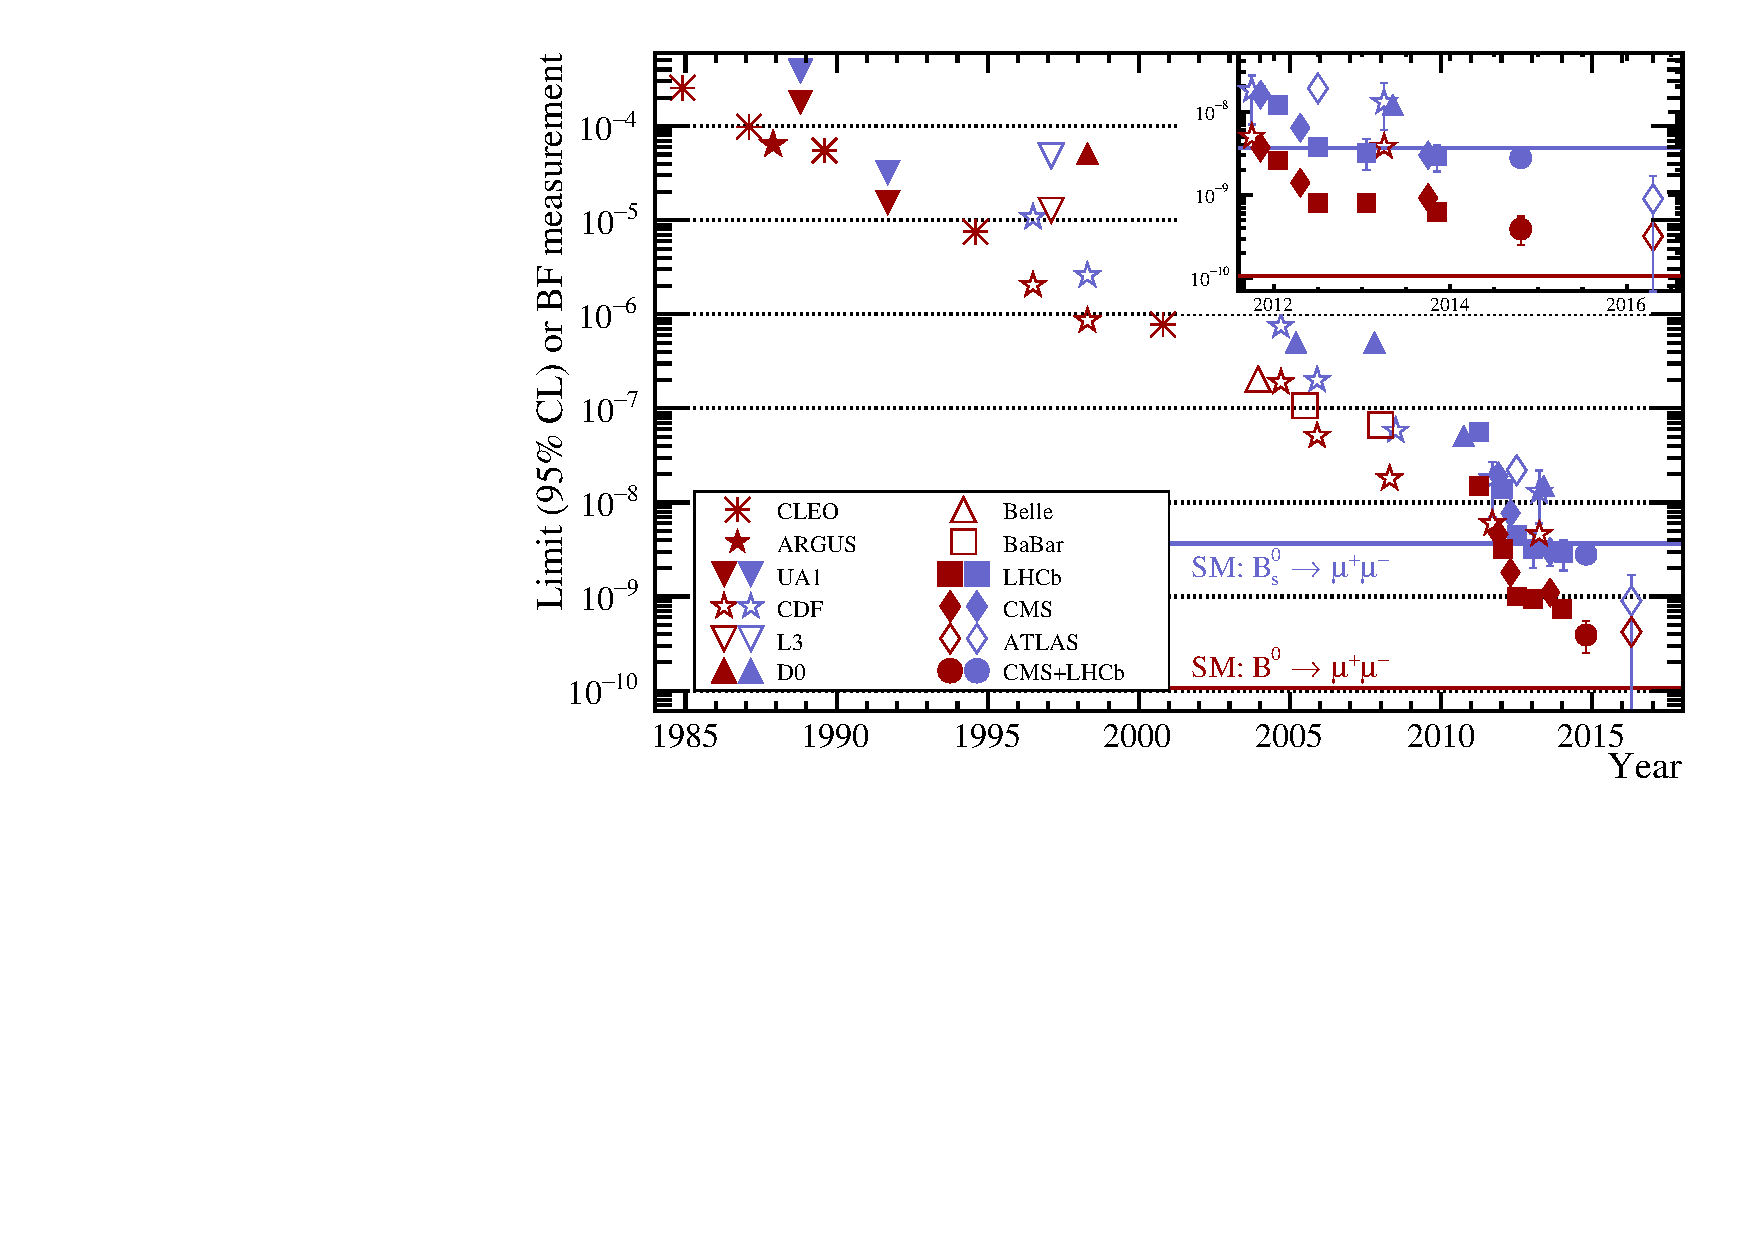
\includegraphics[width=0.8\textwidth]{./Figs/Introduction/95_CL.pdf}
    \caption{Results from searches for \bdmumu (red) and \bsmumu (purple) decays. Upper limits are shown without error bars at the 95$\%$ confindence level. The figure is from reference~\cite{CMS:2014xfa} but updated to include the latest ATLAS result~\cite{Aaboud:2016ire}.}
    \label{fig:bmumu_history}
\end{figure}

The first evidence for \bsmumu decays was found in 2012 by the LHCb experiment~\cite{Aaij:2012nna}. Since then,
the LHCb experiment has measured the \bsmumu \BF to be $\mathcal{B}(B^{0}_{s} \to \mu^+ \mu^-) = (2.9^{+1.1}_{-1.0})\times 10^-9$ at a statistical significance of 4.0$\sigma$ and placed a upper limit on the \bdmumu \BF of $\mathcal{B}(B^{0} \to \mu^+ \mu^-) < 7.4 \times 10^{-10}$ at the 95$\%$ confidence level~\cite{Aaij:2013aka}. The measurements were performed using data collected during 2011 and 2012 at the centre-of-mass energies of 7 and 8 TeV, respectively. Searches for \bmumu decays performed by the CMS experiment using data recorded in the same time period corroborated the results from the results from the LHCb experiment. Producing a measurement of the \bsmumu \BF of $\mathcal{B}(B^{0}_{s} \to \mu^+ \mu^-) = (3.0^{+1.0}_{-0.9})\times 10^-9$ at with a statistical significance of 4.3$\sigma$ and placing a limit on the \bdmumu BF of $\mathcal{B}(B^{0} \to \mu^+ \mu^-) < 1.1 \times 10^{-9}$ at the 95$\%$ confidence level~\cite{Chatrchyan:2013bka}. 
The combined analysis of the CMS and LHCb data sets resulted in the first observation of \bsmumu decays and the first evidence of \bdmumu~\cite{CMS:2014xfa}. The measured branching fractions were measured as
\begin{equation}
\mathcal{B}(B^{0}_{s} \to \mu^+ \mu^-)_{CMS + LHCb}  = 2.8^{+0.7}_{-0.6} \times 10^{-9}
\end{equation}
\begin{equation}
\mathcal{B}(B^{0} \to \mu^+ \mu^-)_{CMS + LHCb}  = 3.9^{+1.6}_{-1.4} \times 10^{-10}
\end{equation}
with a statistical significance of 6.2 $\sigma$ for the \bs mode and 3.0 $\sigma$ for the \bd. The ATLAS experiment also searched for \bmumu decay using data collected during the same period~\cite{Aaboud:2016ire}, measuring the \bsmumu \BF as 
\begin{equation}
\mathcal{B}(B^{0}_{s} \to \mu^+ \mu^-)_{ALTAS}  = 0.9^{+1.1}_{-0.8} \times 10^{-9}
\end{equation}
with a statistical significance of 2~$\sigma$. An upper limit was placed on the \bdmumu decay of $\mathcal{B}(B^{0}_{s} \to \mu^+ \mu^-) >4.2 \times 10^{-10}$ at the 95 $\%$ confidence level.
Although it was hoped that large deviations from the SM predictions would be found in these decays this has not been observed. 
All the measured values are consistent with the expectations of the SM and have enabled constraints to be placed on the parameter space available for new physics models. Nevertheless, the precision of the measurements allows plenty of room for NP effects to be revealed. Furthermore there is some tension between both the separate measurements and each measurement and the SM prediction as shown in Figure~\ref{fig:contour}. 
\begin{figure}[htbp]
    \centering
        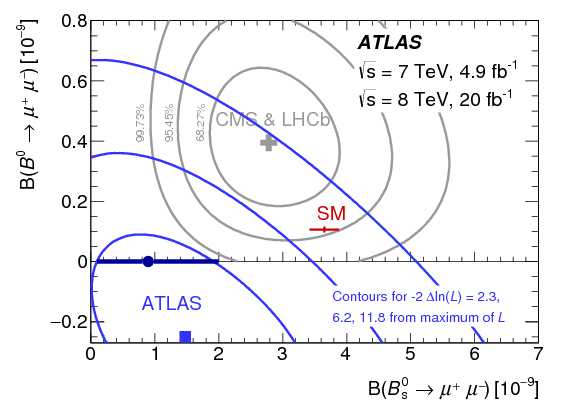
\includegraphics[width=0.8\textwidth]{./Figs/Introduction/contour_plot.png}
        \caption{Measurements of the \bdmumu \BF and \bsmumu \BF from the ATLAS experiment and the combined analysis of CMS and LHCb data alongside the predictions of the SM~\cite{Aaboud:2016ire}. The measurements were performed using data collected during 2011 and 2012 and centre-of-mass energies of 7 and 8~\tev, respectively.}
        \label{fig:contour}
\end{figure}
%The measurements have enabled strong constraints to be placed on the parameter space available for new physics models~\cite{} but the precision of the measurements still allows plenty of room for NP effects to be revealed. 
Therefore the study of \bmumu decays continues to be an very interesting topic in the search for NP effects. 

The data collected during Run 2 of the LHC, where the centre-of-mass energy of $pp$ collisions is increased to 13 TeV, will enable more precise measurements of the \BFs of these decays to be made. 
Furthermore the observation of \bsmumu decays opens the way for other properties of this decay to be studied. In particular the effective lifetime of \bsmumu decays provides a complementary search for NP effects to the \BF measurement, the presence of new physics effects could be revealed in either both or only one of these measurements. The search for \bsmumu decays is over and the study of this decay has begun.



This dissertation documents the latest study of \bmumu decays at the LHCb experiment. The measurements of the \bmumu \BF and the \bsmumu effective lifetime are presented using data collected during $pp$ collisions with centre-of-mass energies of 7, 8 and 13~\tev. The theoretical motivation for studying these decays is given in Chapter~\ref{sec:theory_chptr} and the LHC and LHCb experiment are described in Chapter~\ref{CERN_LHC_LHCb}. The criteria used to identify these decays in the data collected by the LHCb experiment are detailed in Chapter~\ref{selection_chapter} and the measurement of the \BF is briefly covered in Chapter~\ref{sec:BFanalysis}. The measurement of the effective lifetime is discussed in Chapter~\ref{sec:lifetimemeasurement} and the systematic uncertainties on this measurement are given in Chapter~\ref{sec:systematics}. Finally a summary of the results and prospects for future measurements of \bmumu decays are given in Chapter~\ref{sec:summaryandoutlook}.


\chapter[Theory of $B\to \mu^+ \mu^-$ decays; the Standard Model and beyond]{Theory of \boldmath{$B\to \mu^+ \mu^-$} decays; the Standard Model and beyond}
\label{sec:theory_chptr}
This Chapter describes the theoretical motivation for the study of \bmumu decays. 
The description of these decays within the SM framework is presented in Section~\ref{sec:bsmumu_in_SM} and the determination of the theoretical predictions of \BFs is outlined in Section~\ref{sec:BFdef}.
The discussion of the theoretical \BFs is based on references~\cite{Blake:2016olu,Anikeev:2001rk}. 
Quark mixing leads to oscillations of a \bs to a \barbs over time and a difference between the values of the predicted and measured \bsmumu \BFs. These oscillations and the influence on the \BFs values are described in Section~\ref{sec:quarkmaixing} and follows the material in refereneces~\cite{Dunietz:2000cr, Anikeev:2001rk,Nierste:2009wg}. 
A new parameter, \ADG, arises from the \bs - \barbs oscillations and it can be measured through the effective lifetime of \bsmumu decays as described in Section~\ref{sec:ADG_EL}. The SM predictions for \BFs and the effective lifetime are given in Section~\ref{sec:SM_predictions} and the ways in which NP can influence these observables is briefly discussed in Section~\ref{sec:NPmodels}.



\section[$B^0_{(s)}\to \mu^+ \mu^-$ decays in the Standard Model]{\boldmath{$B^0_{(s)}\to \mu^+ \mu^-$} decays in the Standard Model}
\label{sec:bsmumu_in_SM}
%Prehaps I should mention anti-particles earlier?
In the SM, quarks and anti-quarks can be combined in pairs to form mesons that are held together by the strong force. The neutral $B$ mesons, \bd and \bs, are made up of a $\bar{b}$ quark combined with a $d$ quark for the \bd and an $s$ quark for the \bs. Their anti-particles, \barbd and \barbs, are formed by swapping over which quark flavour in the pair is the anti-quark. These particles are unstable and exist for $\sim10^{-12}$~s before decaying into leptons, lighter mesons or a combination of both. One decay mode is when the \bsd decays into two oppositely charged muons as \bmumu~\footnote{\bmumu refers to both the particle and anti-particle decays of the \bd and \bs unless otherwise specified.}. This decay mode occurs very rarely in the SM compared to other decay modes of the \bsd, the suppression of this mode arises from several different sources.

The composite quarks of a \bsd both have the same charge, therefore in the decay \bmumu only quark flavour and not quark charge changes. This type of decay is called a flavour changing neutral current (FCNC). These decays must proceed via the weak force because it is the only interaction in which quark flavour is not conserved via the exchange of a $W$ boson. However, FCNCs are forbidden in the SM to occur at the tree level by the GIM mechanism~\cite{PhysRevD.2.1285}. Therefore \bmumu decays proceed via $W$-box and $Z^0$-penguin diagrams as shown in Figure~\ref{fig:SM_diag}.

\begin{figure}[htbp]
    \centering
        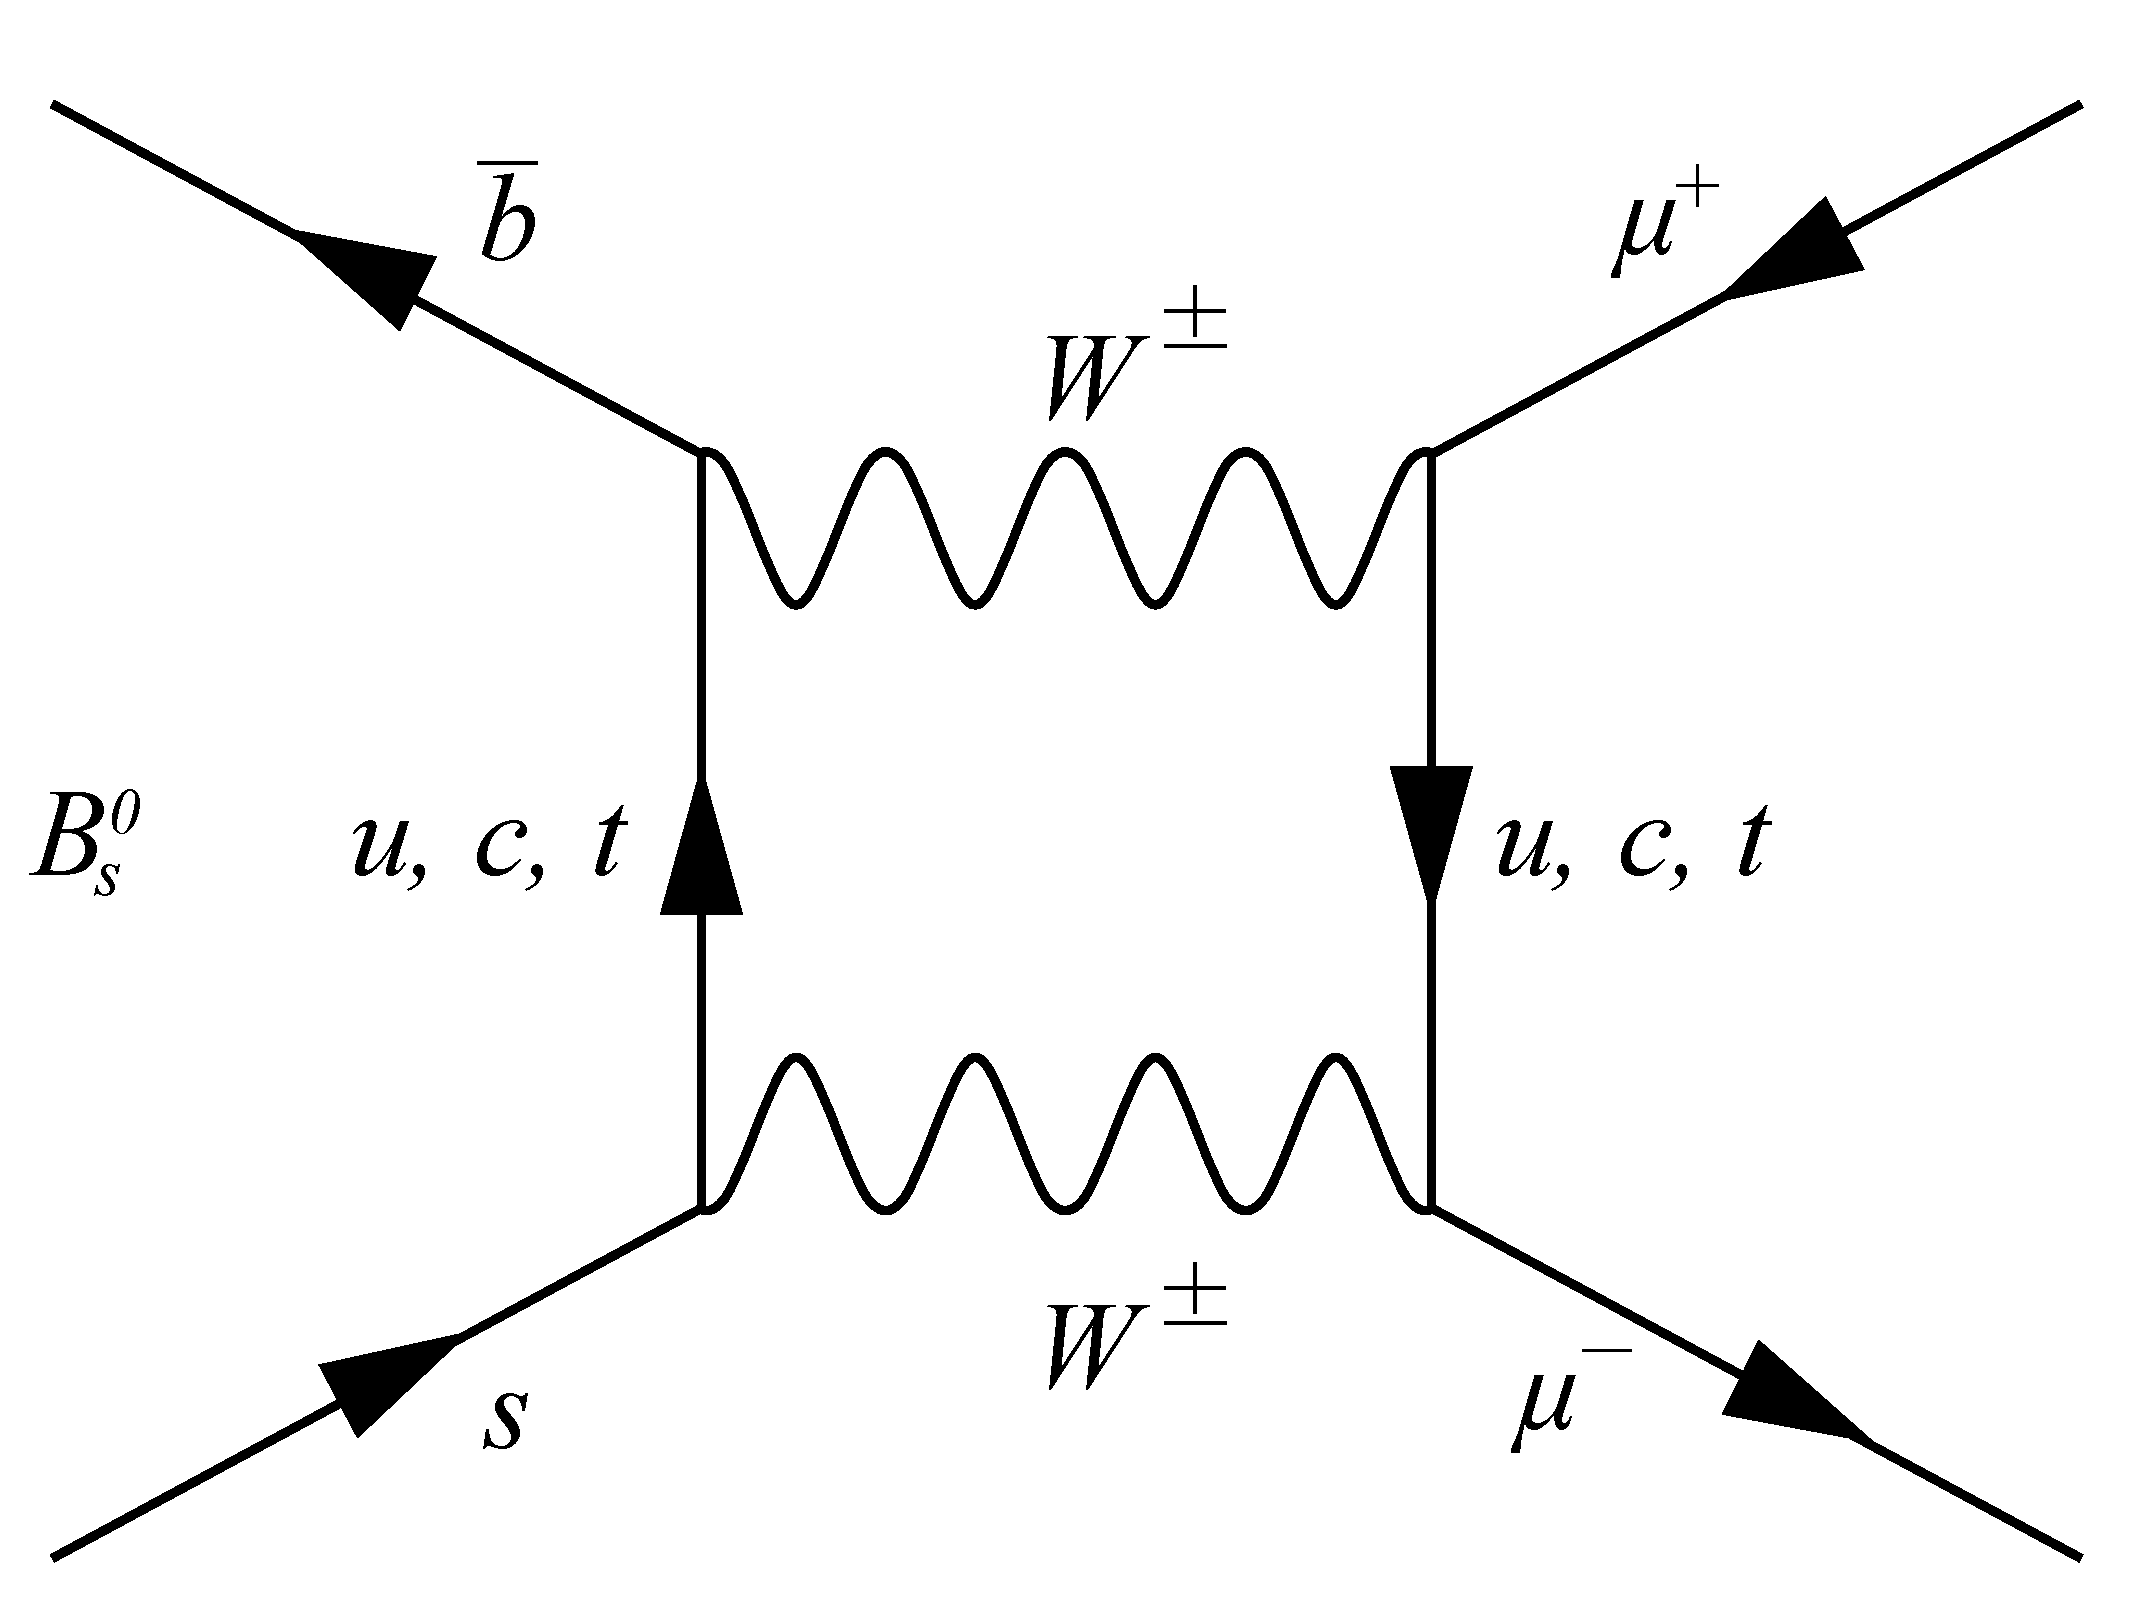
\includegraphics[width=0.4\textwidth]{./Figs/Theory/W_diagram.pdf}
        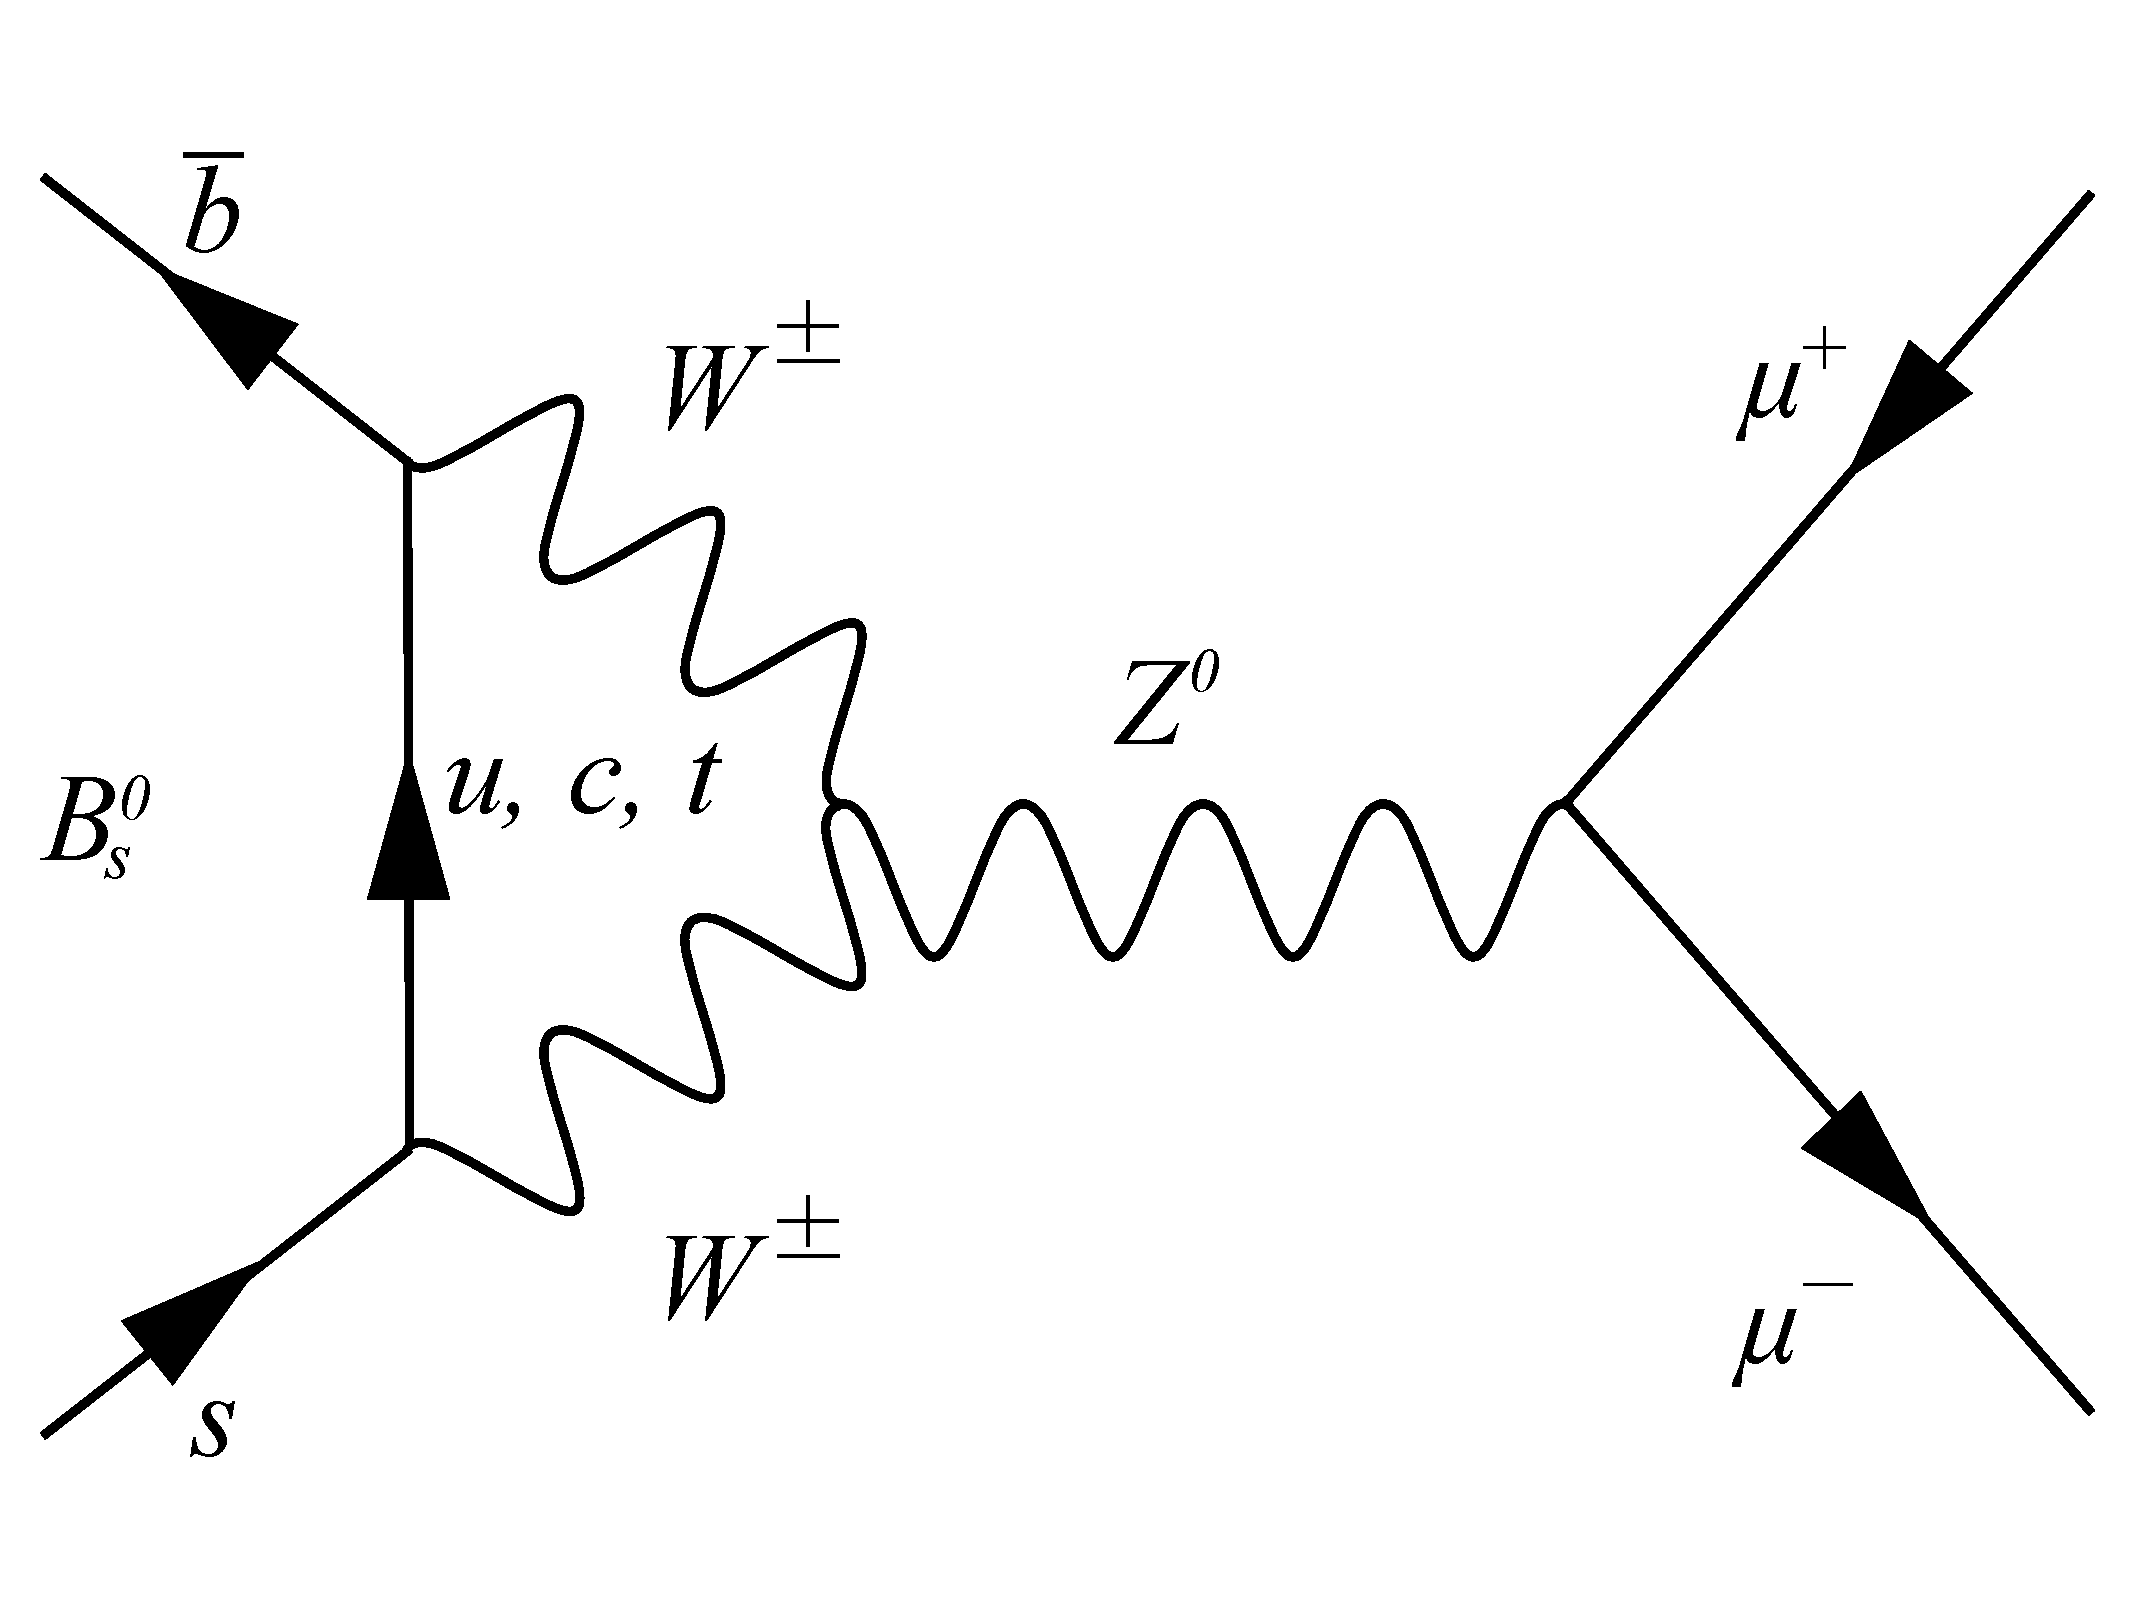
\includegraphics[width=0.4\textwidth]{./Figs/Theory/Z0_penguin_v1.pdf}
        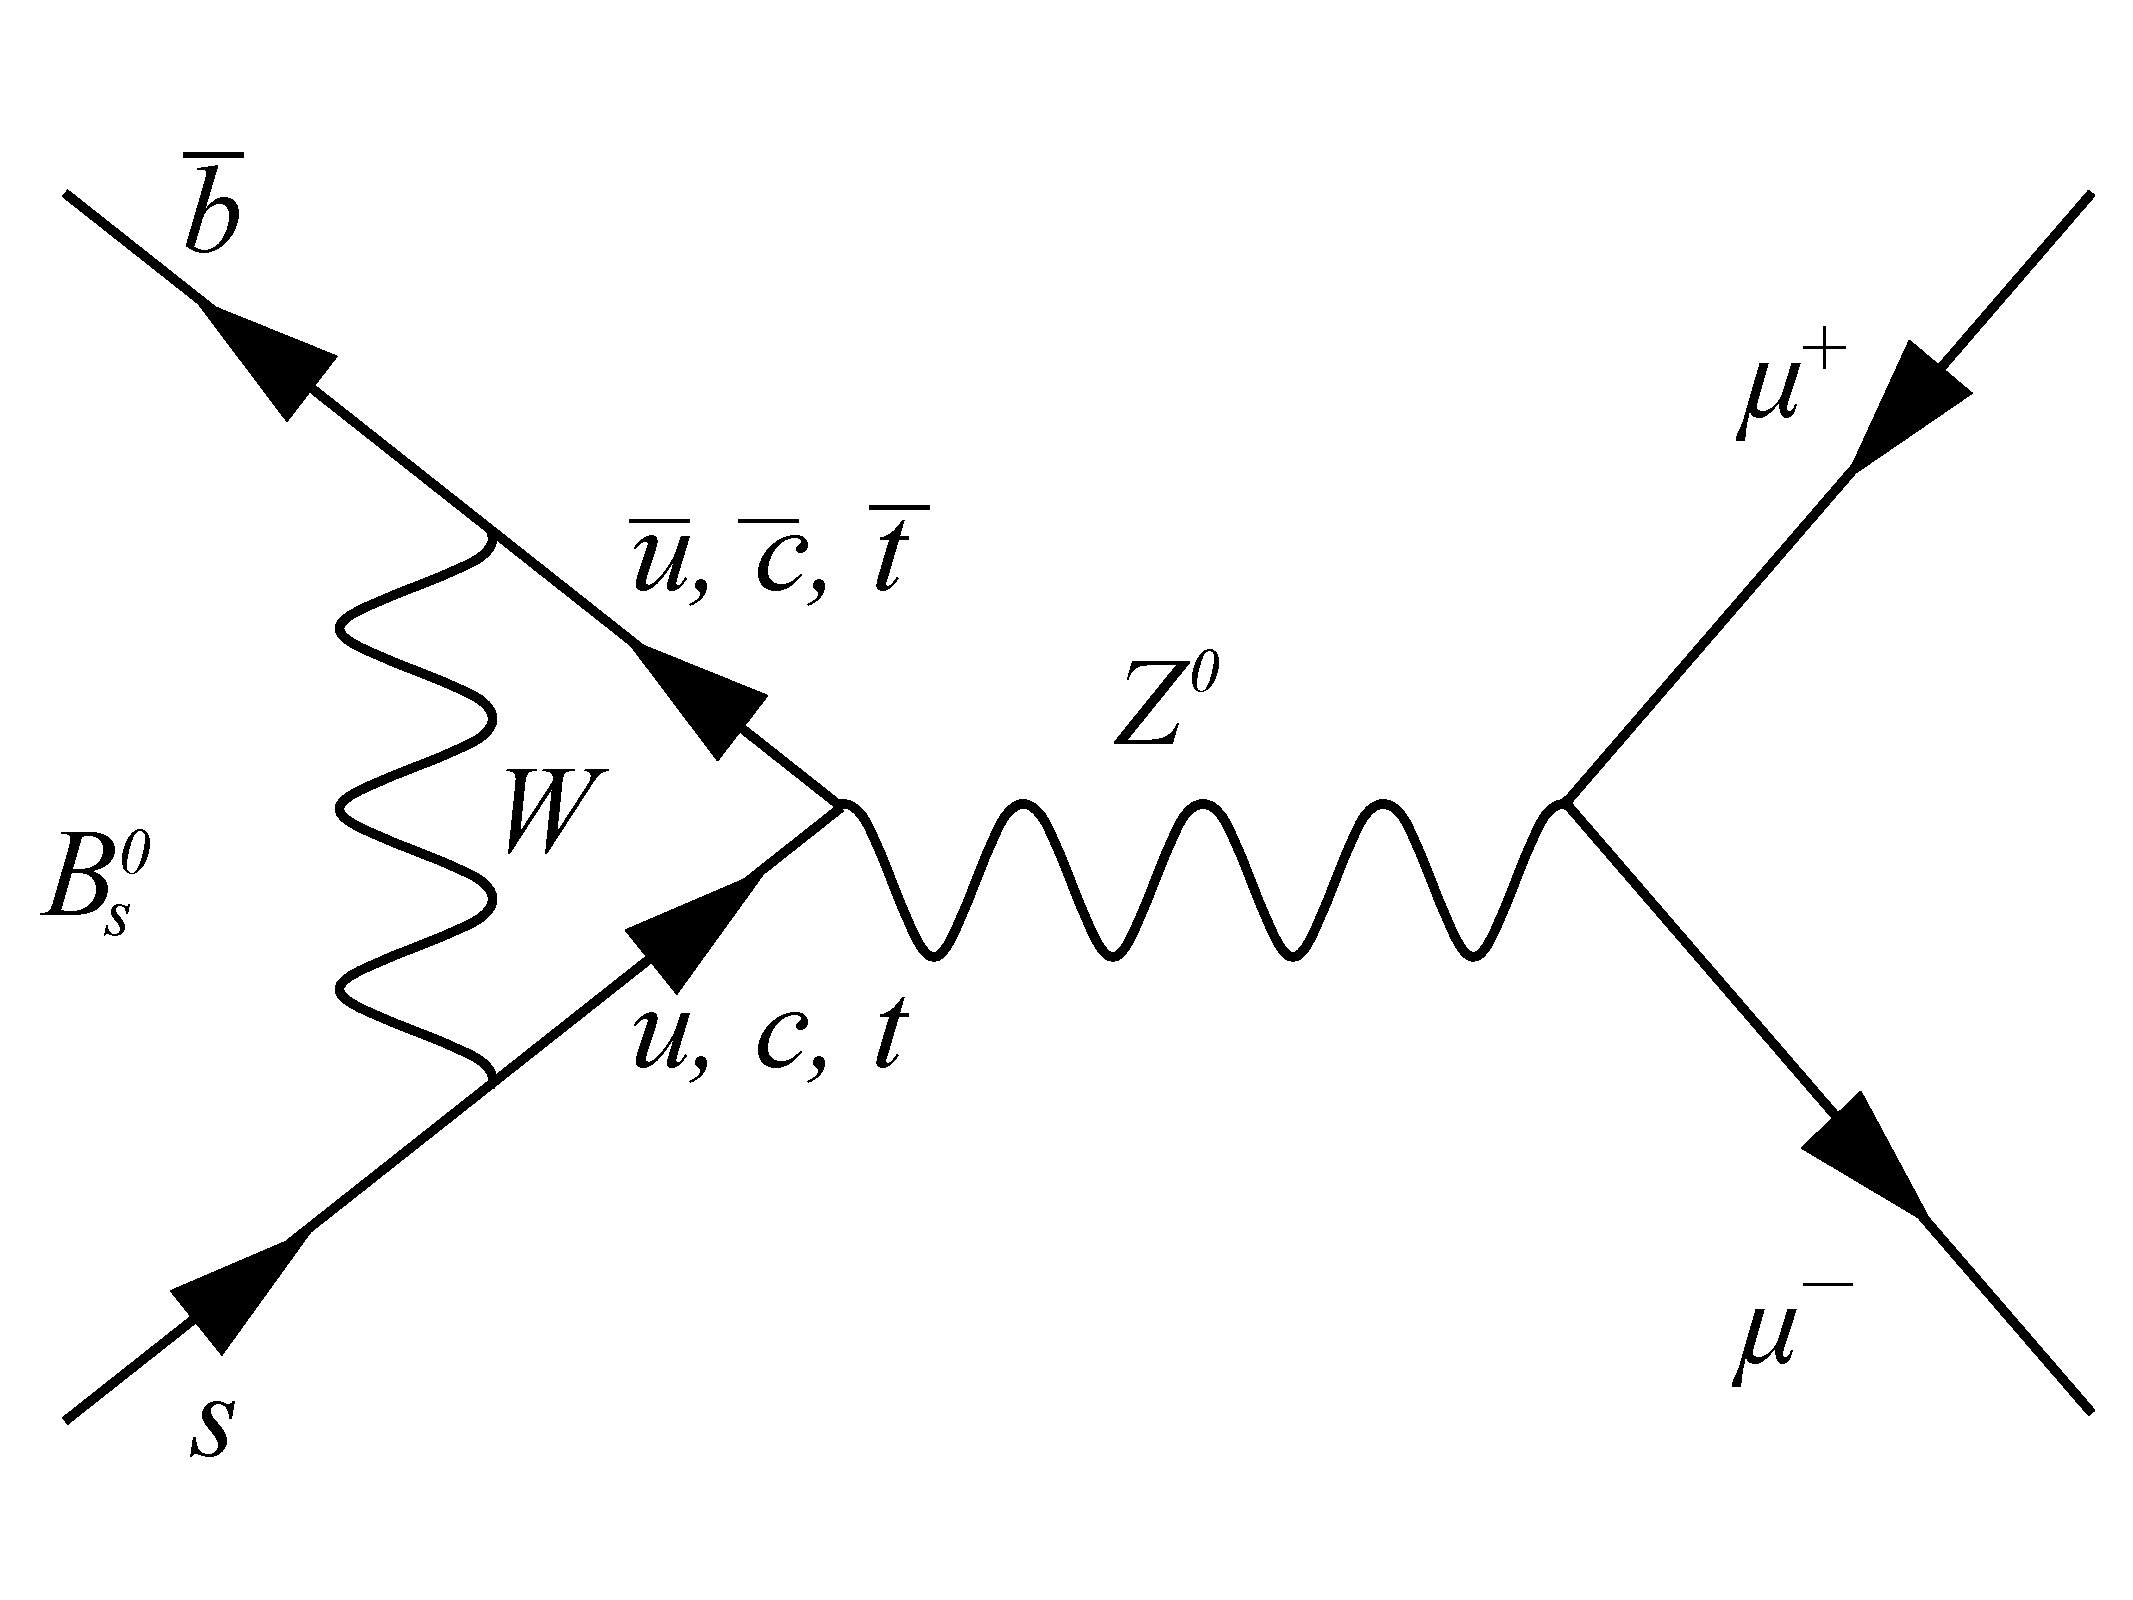
\includegraphics[width=0.4\textwidth]{./Figs/Theory/Z0_penguin_v2.pdf}
    \caption{Feynman diagrams for \bsmumu decays in the SM via $W$-box and $Z^0$-penguin processes. The same diagrams apply to \bdmumu decays but the $s$ quark is exchanged for a $d$ quark.}
    \label{fig:SM_diag}
\end{figure}

The decays can also proceed via Higgs-penguin diagrams however the contributions from these diagrams are negligible. %within the SM.
The lack of \bmumu decays at the tree level causes them to be suppressed compared to other \bsd decay modes that can occur at the tree level.

%{\it I think that this needs to be re-worded.

%Although the weak force allows quark flavour to change the coupling strengths between different quark flavours are not all the same magnitude. The coupling strengths are described by the CKM matrix. Quarks can Quarks fall into three families; $u$ and $d$, $c$ and $s$, $t$, and $b$. They can also be separated into two types depending on their charge; up-type quarks include $u$, $c$ and $t$, down-type quarks include $d$, $s$ and $b$. The weak force couples up-type quarks to the weak eigenstates of the down-type quark in the same family with the same strength. The weak quark eigenstates are not the same as the mass eigenstates and the two types of states are related via the CKM matrix as
%}

%{\it where $d^', s^'$ and $b^'$ are weak eigenstates and $d, s$ and $b$ are mass eigenstates. The CKM matrix is a unitary matrix, which ensures no tree level FCNCs occur, with complex elements that give the coupling strengths of different quarks, for example the amplitude of a $u$ quark changing into a $d$ quark is proportional to $|V_{ud}|$.}


Although the weak force allows quark flavour to change the coupling strengths between different quark flavours are not all the same magnitude. The coupling strengths are described by the CKM matrix. Quarks can be separated into two types depending on their charge; up-type quarks include $u$, $c$ and $t$, down-type quarks include $d$, $s$ and $b$. The weak force couples all up-type quarks to the weak eigenstate of the down-type quark in the same family with the same strength. Where the quark families are; $u$ and $d$, $c$ and $s$, $t$, and $b$. The weak quark eigenstates are not the same as the mass eigenstates and the two types of states are related via the CKM matrix~\cite{PhysRevLett.10.531,doi:10.1143/PTP.49.652} as
\begin{equation}
\begin{pmatrix}
d'\\
s'\\
b'
\end{pmatrix}
= 
\mathbf{V_{CKM}}
\begin{pmatrix}
d\\
s\\
b
\end{pmatrix} =
 \begin{pmatrix}
   V_{ud} & V_{us} & V_{ub} \\
   V_{cd} & V_{cs} & V_{cb} \\
   V_{td} & V_{ts} & V_{tb}
 \end{pmatrix}
\begin{pmatrix}
d\\
s\\
b
\end{pmatrix}
\label{eq:CKMA}
\end{equation}
where $d'$, $s'$ and $b'$ are weak eigenstates and $d$, $s$ and $b$ are mass eigenstates. The CKM matrix is a unitary matrix with complex elements which ensures no tree level FCNCs occur. Each element of the matrix gives the coupling strengths of transitions between the mass eigenstates of quarks, for example the amplitude of a $u$ quark changing into a $d$ quark is proportional to $|V_{ud}|$.

The difference in the coupling strength sizes can illustrated through the Wolfenstein parametrisation of the CKM matrix~\cite{PhysRevLett.51.1945}, which parametrises the matrix elements in powers of the small parameter of $\lambda = 0.22 \approx |V_{us}|$. The CKM matrix then becomes
\begin{equation}
\mathbf{V_{CKM}} =
 \begin{pmatrix}
 1 - \frac{1}{2}\lambda^2 & \lambda & \lambda^3 A (\rho - i \eta) \\
 - \lambda                & 1 - \frac{1}{2}\lambda^2 & \lambda^2 A \\
 \lambda^3 A (1 - \rho- i \eta) & -\lambda^2 A & 1
 \end{pmatrix} + \mathcal{O}(\lambda^4).
\label{eq:CKMB}
\end{equation}
This parametrisation shows that the CKM matrix is almost diagonal. For a \bmumu decay to occur one off diagonal element in needed to described the quark transitions in Figure~\ref{fig:SM_diag}. Therefore introducing an additional source of suppression to the decay. 

The internal quark lines in Figure~\ref{fig:SM_diag} can have contributions from $u$, $c$ and $t$ quarks. However in the SM the contributions from $u$ and $c$ quarks are negligible when compared to the $t$ quark. This is due to the large $t$ quark mass and because the coupling strength of the $b$ quark to any quark except the $t$ is extremely small.


The final source of suppression of \bmumu decays comes from the helicities of the muons in the final state. Both \bd and \bs are spin zero particles and for angular momentum to be conserved in the decay the spins of the two muons must be oppositely aligned. This leads to the muons having opposite helicities. % Therefore the production of one of the muons will always be suppressed.
The weak force only couples to left-handed particle states and right-handed anti-particle states. In the high energy limit where particles are massless, negative helicity states are equal to left-handed states and positive helicity states are equal to right-handed states.
Therefore if the muons were massless the weak interaction could only produce a $\mu^-$ and a $\mu^+$ with opposite helicities which cannot conserve angular momentum in \bmumu decays.
Muon are not massless therefore \bmumu decay can occur but are suppressed because $m_{\mu} \ll M_{B_{(s)}$~\cite{Olive:2016xmw} leading to one of the helicity states of the muons always being disfavoured.

Overall \bmumu decays are highly suppressed within the framework of the SM compared to other decay modes of \bsd mesons. Therefore these decays offer excellent processes in which to search for NP because the contribution of BSM theories to these decay rates can be at a similar order of magnitude to those from the SM.

\section[\bmumu Branching Fraction]{\boldmath{\bmumu} Branching Fraction}
\label{sec:BFdef}
The \BF of a particle decay offers an excellent observable through which predictions of the SM can be compared to measured values. The \bmumu \BF is defined as the fraction of the total number of \bsd particles that decay into two muons. It can be calculated from the decay rate, which is the probability per unit time that a \bsd decays into two muons, as
\begin{equation}
\mathcal{B}(B^0_{(s)} \to \mu^+ \mu^-) \equiv \frac{\Gamma(B^0_{(s)}(t) \to \mu^+ \mu^-) + \Gamma(\
\overline{B}^0_{(s)}(t) \to \mu^+ \mu^-)}{\Gamma(B^{0}_{(s)}) + \Gamma(\overline{B}^{0}_{(s)}) }
\end{equation}

The SM predictions are calculated from the `prompt' decay rate that ignore any evolution with time of the \bsd particles. The \BFs are calculated using~\cite{DeBruyn:2012wj} 
\begin{equation}
\mathcal{B}(B^0_{(s)} \to \mu^+ \mu^-)_{\mathrm{th}} = \frac{ \tau_{B_{(s)}} }{2} \langle \Gamma(B^0_{(s)}(t) \to \mu^+ \mu^-) \rangle \big{|}_{t=0}
\label{sec:BF_prompt}
\end{equation}
where $\tau_{B_{(s)}$ is the mean lifetime of the \bsd and $\langle \Gamma(B^0_{(s)}(t) \to \mu^+ \mu^-) \rangle$ is defined as
\begin{equation}
\langle \Gamma(B^0_{(s)}(t) \to \mu^+ \mu^-) \rangle = \Gamma(B^0_{(s)}(t) \to \mu^+ \mu^-) + \Gamma(\overline{B}^0_{(s)}(t) \to \mu^+ \mu^-).
\end{equation}
The \BFs are calculated this way to enable easy comparison of different $B$ meson \BFs including \bd, \bs and $B^+$~\cite{DeBruyn:2012wj}.

The prompt decay rate is evaluated from Fermi's golden rule, relating the decay rate  to the transition amplitude, $\left|\mathcal{M}(B^0_{(s)} \to \mu^+ \mu^-)\right|$, and the kinematics of the decay to give~\cite{Tolk:2148631}
\begin{equation}
\Gamma(B^0_{(s)}(t) \to \mu^+ \mu^-)\big{|}_{t=0} = \frac{1}{16\pi} \frac{1}{M_{B_{(s)}}} \sqrt{1 -4 \left (\frac{m_{\mu}}{M_{B_{(s)}}} \right )^2} \left|\mathcal{M}(B^0_{(s)} \to \mu^+ \mu^-)\right|^2
\label{sec:FGR}
\end{equation}
where $m_{\mu}$ and $M_{B_{(s)}}$ are the masses of the muon and the \bsd, respectively. The factor of $\right( \frac{m_{\mu}}{M_{B_{(s)}}}\left)$ comes from the helicity suppression discussed in Section~\ref{sec:bsmumu_in_SM}.


Weak decays like \bmumu include interactions that occur at different energy scales, from the weak propagators at $M_W \approx 80$~\gevcc to the strong coupling in the \bsd meson at $\Lambda_{QCD} \sim 0.2$~\gev~\cite{Olive:2016xmw}. %This enable the Operator Product Expansion~\cite{} method to be used to construct the effective Hamiltonian, $\mathcal{H}_{eff}$, and calculate the transition amplitude $|\matcal{M}(B^0_{(s)} \to \mu^+ \mu^-)| = \langle \mu \mu | \mathcal{H}_{eff} | B^0_{(s)} \rangle$. The effective Hamiltonian divides the interaction into two energy levels with the structure
The Operator Product Expansion~\cite{PhysRev.179.1499,Wilson1972} is used to create the effective hamiltonian, $\mathcal{H}_{eff}$, which splits the interaction into two energy levels. The transition amplitude then becomes 
\begin{equation}
|\matcal{M}(B^0_{(s)} \to \mu^+ \mu^-)| \equiv \langle \mu \mu | \mathcal{H}_{eff} | B^0_{(s)} \rangle  = \frac{G_F}{\sqrt{2}} \displaystyle\sum_{i} V^i_{CKM} \langle \mu \mu | \mathcal{C}(\mu)_i \mathcal{O}(\mu)_i | B^0_{(s)} \rangle
\label{sec:eff_hamil_def}
\end{equation}
where $G_F$ is the Fermi coupling constant, $V_{CKM}^i$ are CKM matrix elements, $\matcal{C}_i$ are Wilson coefficients and $\mathcal{O}_i$ are local operators. The energy scale $\mu$ separates the two energy levels in the interaction. The Wilson coefficients describe short scale processes with energies above $\mu$. This incorporates the internal structure and loops of Feynman diagrams leading to the dependance of Wilson coefficients on the $W^{\pm}$, $Z^0$, $H^0$ and $t$ quark masses. The long distance processes are described by the local operators $\mathcal{O}_i$ for energies less than $\mu$. The local operators link the initial and final states of the decay. % indendant of the internal structure of the interaction. 
Wilson coefficients can be calculated using perturbation theory however this cannot be used for the local operators which can lead to large theoretical uncertainties on their values. The choice of $\mu$ is arbitrary however the final transition amplitude must be independent of $\mu$, often the mass of the decaying particle is used. 

%The Operator Product Expansion can be used to describe weak decays with different initial and final states as well as internal structure. 
In the effective Hamiltonian in Equation~\ref{sec:eff_hamil_def} the CKM matrix elements are factored out of the Wilson coefficients and operators, therefore the same coefficients and operators can be used to describe the \bd and \bs decays.
The effective Hamiltonian for \bmumu decays is~\cite{DeBruyn:2012wk}
\begin{equation}
\mathcal{H}_{eff} = -\frac{G_F \alpha}{\sqrt{2\pi}} V_{tq}^{*}V_{tb} \displaystyle\sum_{i}^{10,S,P} (\matcal{C}_i\matcal{O}_i + \matcal{C}^{'}_{i}\matcal{O}_{i}^{'})
\label{eq:eff_hamil_bmumu}
\end{equation}
where $\alpha$ is the fine structure constant and $q$ corresponds to the $d$ quark in the \bd or the $s$ quark in the \bs. Terms proportional to $V^*_{cq}V_{cb}$ and $V^*_{cq}V_{ub}$ neglected because they are negligible. The operators that can contribute to the \bmumu effective Hamiltonian due to the initial and final decay states are
\begin{align}
 \mathcal{Q}_{10}&=(\bar{q}\gamma^{\mu}P_{L}b)(\bar{l}\gamma_{\mu}\gamma_{5}l), &\qquad
 \mathcal{Q}_{10}^{(')}&= (\bar{q}\gamma^{\mu}P_{R}b)(\bar{l}\gamma_{\mu}\gamma_{5}l), \\
 \mathcal{Q}_{S}&= m_{b}(\bar{q}P_{R}b)(\bar{l}l),  &\qquad
\mathcal{Q}_{S}^{(')}&= m_{b}(\bar{q}P_{L}b)(\bar{l}l), \\
 \mathcal{Q}_{P}&= m_{b}(\bar{q}P_{R}b)(\bar{l}\gamma_{5}l), &\qquad
 \mathcal{Q}_{P}^{(')}&= m_{b}(\bar{q}P_{L}b)(\bar{l}\gamma_{5}l).
\end{align}
%\begin{eqnarray}
% \mathcal{Q}_{10}&=(\bar{q}\gamma^{\mu}P_{L}b)(\bar{l}\gamma_{\mu}\gamma_{5}l),  \qquad
% \mathcal{Q}_{10}^{(')}&= (\bar{q}\gamma^{\mu}P_{R}b)(\bar{l}\gamma_{\mu}\gamma_{5}l), \\
% \mathcal{Q}_{S}&= m_{b}(\bar{q}P_{R}b)(\bar{l}l),  \qquad
%\mathcal{Q}_{S}^{(')}&= m_{b}(\bar{q}P_{L}b)(\bar{l}l), \\
% \mathcal{Q}_{P}&= m_{b}(\bar{q}P_{R}b)(\bar{l}\gamma_{5}l),  \qquad
% \mathcal{Q}_{P}^{(')}&= m_{b}(\bar{q}P_{L}b)(\bar{l}\gamma_{5}l) 
%\label{eq:operators}
%\end{eqnarray}
The operator $\mathcal{O}_{10}$ encompasses the only significant contributions in the SM that come from $W$-box and $Z^0$ penguin diagrams. The operator $\mathcal{O}_{10}^'$ describes the equivalent interactions as $\mathcal{O}_{10}$ but for right handed currents that are forbidden in the SM. %, de and $\mathcal{O}_{10}^'$ does not contribute in the SM because is describes right handed currents.% which are forbidden in weak interactions in the SM are described by $\mathcal{O}_{10}^'$ and 
 Finally, the operators $\mathcal{O}_{S}^{(')}$ and $\mathcal{O}_{P}^{(')}$ correspond to the exchange of scalar and pseudo-scalar particles which is negligible in the SM. 

The purely leptonic final state of \bmumu decays means that the computation of the transition amplitude can be spilt in two so that all uncertainties arising from the bound \bsd states are encompassed into one parameter, $F_{B_{(s)}}}$, the hadronic decay factor. This leads to a theoretically clean prediction for the \BF.

The \BFs for \bmumu decays can therefore be written as~\cite{Buras:2013uqa}
\begin{equation}
\mathcal{B}(B^{0}_{(s)} \to \mu^{+} \mu^{-})=&\frac{\tau_{B_{(s)}}G_{F}^{4} M_{W}^{4} \sin^{4}\theta_{W} }{8\pi^{5}} \big|\mathcal{C}_{10}^{SM} V^{*}_{tq}V_{tb}\big|^{2} F_{B_{(s)}}M_{B_{(s)}} m_{\mu}^{2} \sqrt{1 - \frac{4m_{\mu}^{2}}{M^{2}_{B_{(s)}}}} (|P|^{2} + |S|^{2})
\label{eq:BF_form}
\end{equation}
where $\theta_W$ is the weak mixing angle and $M_{W}$ the mass of the $W$ boson. The \BF has been parametrised in terms of $\mathcal{C}_{10}^{SM}$, $P$ and $S$, where $\mathcal{C}_{10}^{SM}$ is the SM value of the operator $\mathcal{C}_{10}$ and 
\begin{equation}
P \equiv |P| e^{i\varphi_P} \equiv \frac{\mathcal{C}_{10} - \mathcal{C}_{10}^{'}}{\mathcal{C}_{10}^{SM}} + \frac{M^2_{B_{(s)}}}{2m_{\mu}} \frac{m_b}{m_b + m_q} \frac{\mathcal{C}_{P} - \mathcal{C}_{P}^{'}}{\mathcal{C}_{10}^{SM}} 
\label{eq:P}
\end{equation}
\begin{equation}
S \equiv |S| e^{i\varphi_S} \equiv \sqrt{1- \frac{4m_{\mu}^{2}}{M^{2}_{B_{(s)}}}} \frac{M^{2}_{B_{(s)}}}{2m_{\mu}}  \frac{m_b}{m_b + m_q}  \frac{\mathcal{C}_{S} - \mathcal{C}_{S}^{'}}{\mathcal{C}_{10}^{SM}} 
\label{eq:S}
\end{equation}
In the SM $P=1$ and $S=0$, however the \BFs are parametrised in terms of $P$ and $S$ because BSM theories can significantly alter their values. 
%The dependence of the \BFs on $\mathcal{C}_{10}$ makes \bmumu decays one of the best decays to study this parameter and these decays are also very sensitive to scale particles~\cite{}. 
The presence of scalar particles could increase the \BFs above the SM expectation through $\mathcal{C}_S^{(')}$ leading to $S>0$, also the contributions from scalar particles are not subject to helicity constraints. Pseudoscalar particles can either enhance or suppress the \BFs compared to the SM prediction depending on how the values of $\mathcal{C}_P^{(')}$ interfere with $\mathcal{C}_{10}^{(')}$ in NP models.


As well as the individual \BFs of \bdmumu and \bsmumu decays the ratio of the two \BFs is also an interesting observable. The ratio of \BFs is given by
\begin{equation}
  \mathcal{R} = \frac{\mathcal{B}(B^{0} \to \mu^{+} \mu^{-})}{\mathcal{B}(B^{0}_{s}\to \mu^{+} \mu^{-})} = \frac{\tau_{B}}{\tau_{B_{s}}} \bigg{|} \frac{V_{td}}{V_{ts}} \bigg{|}^{2} \frac{M_{B}^{2}}{M_{B_{s}}^{2}} \sqrt{\frac{1 - \frac{4m_{\mu}^{2}}{M^{2}_{B}}}{1- \frac{4m_{\mu}^{2}}{M^{2}_{B_{s}}}}} 
\label{eq:BF_ratio}
\end{equation}
and the uncertainty on the ratio is less that the individual \BFs because sources of uncertainties including those from Wilson coefficients and $|V_{tb}|$ cancel out. The ratio does not depend on Wilson coefficients and provides an excellent observable to test the flavour structure of the SM and BSM theories.


\section{Quark mixing}
\label{sec:quarkmaixing}
The theoretical prediction for the \bmumu \BFs does not take into account the evolution of the \bsd and \barbsd mesons with time. Once a \bsd is created it will oscillate between the particle and anti-particle states as it propagates through time, the same is true for the \barbsd. Therefore the states that travel through time are a superposition of the \bsd and the \barbsd. These oscillation occurs as the constituents quarks transition between different flavours through the exchange of $W$ bosons as illustrated in Figure~\ref{fig:Oscl_diag}.
\begin{figure}[htbp]
    \centering
        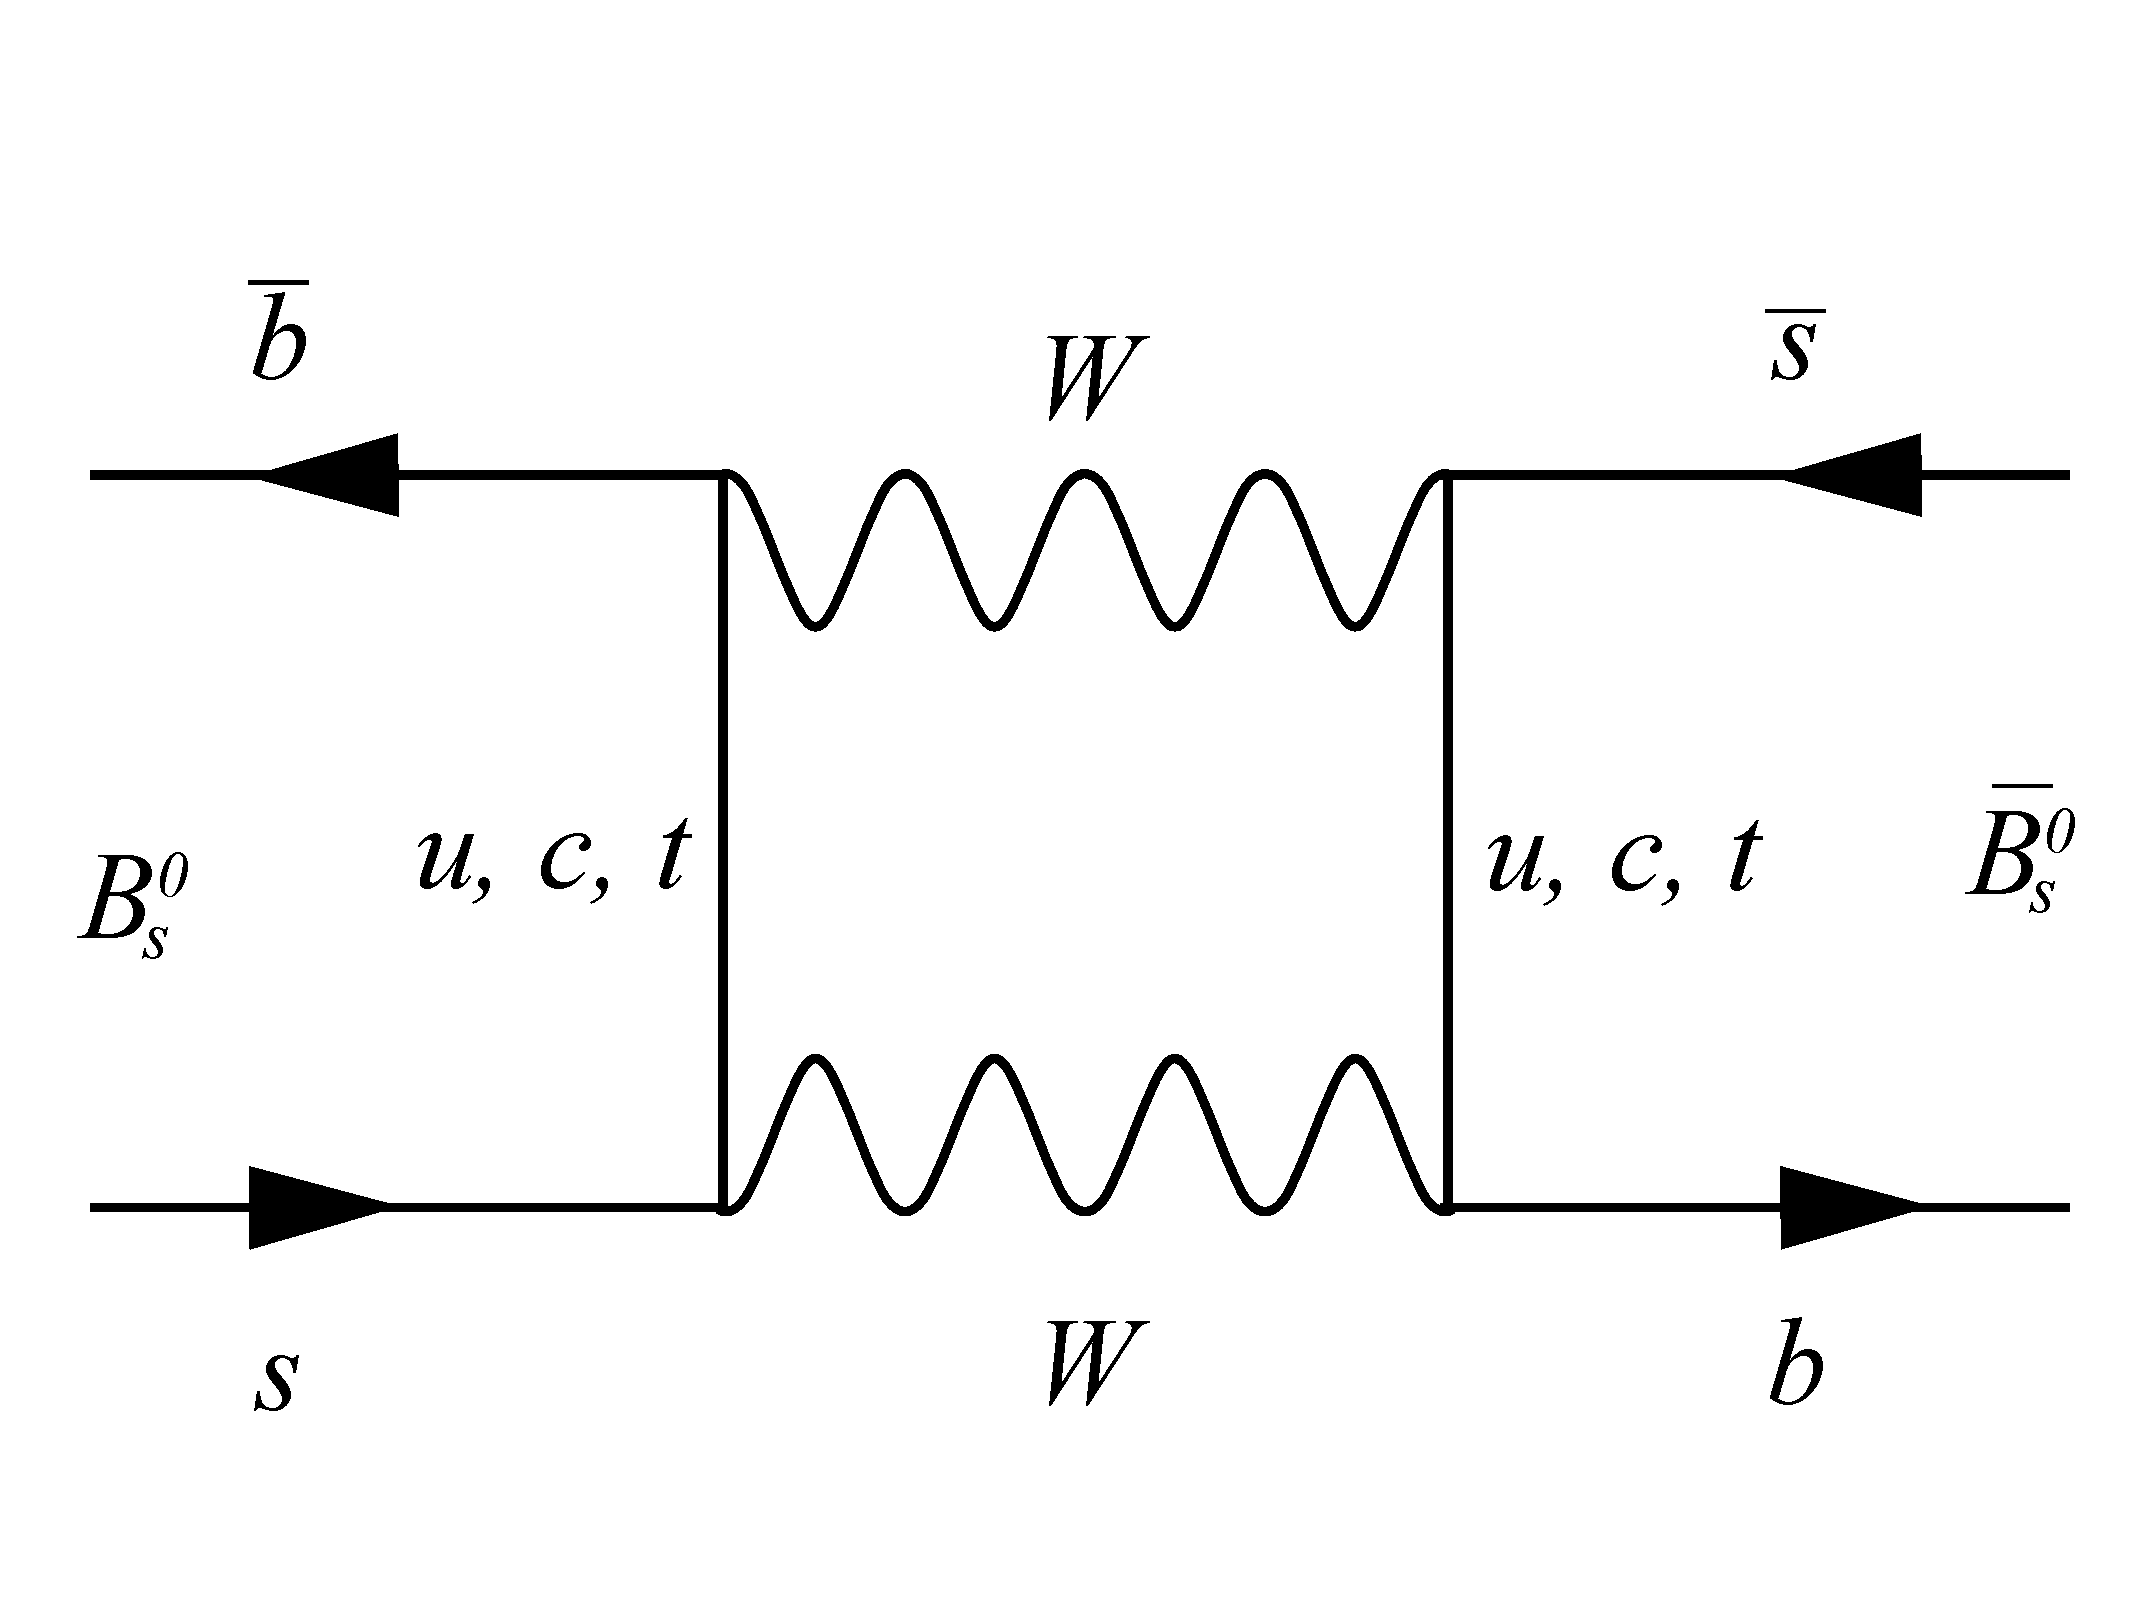
\includegraphics[width=0.5\textwidth]{./Figs/Theory/Oscillation_1.pdf}
        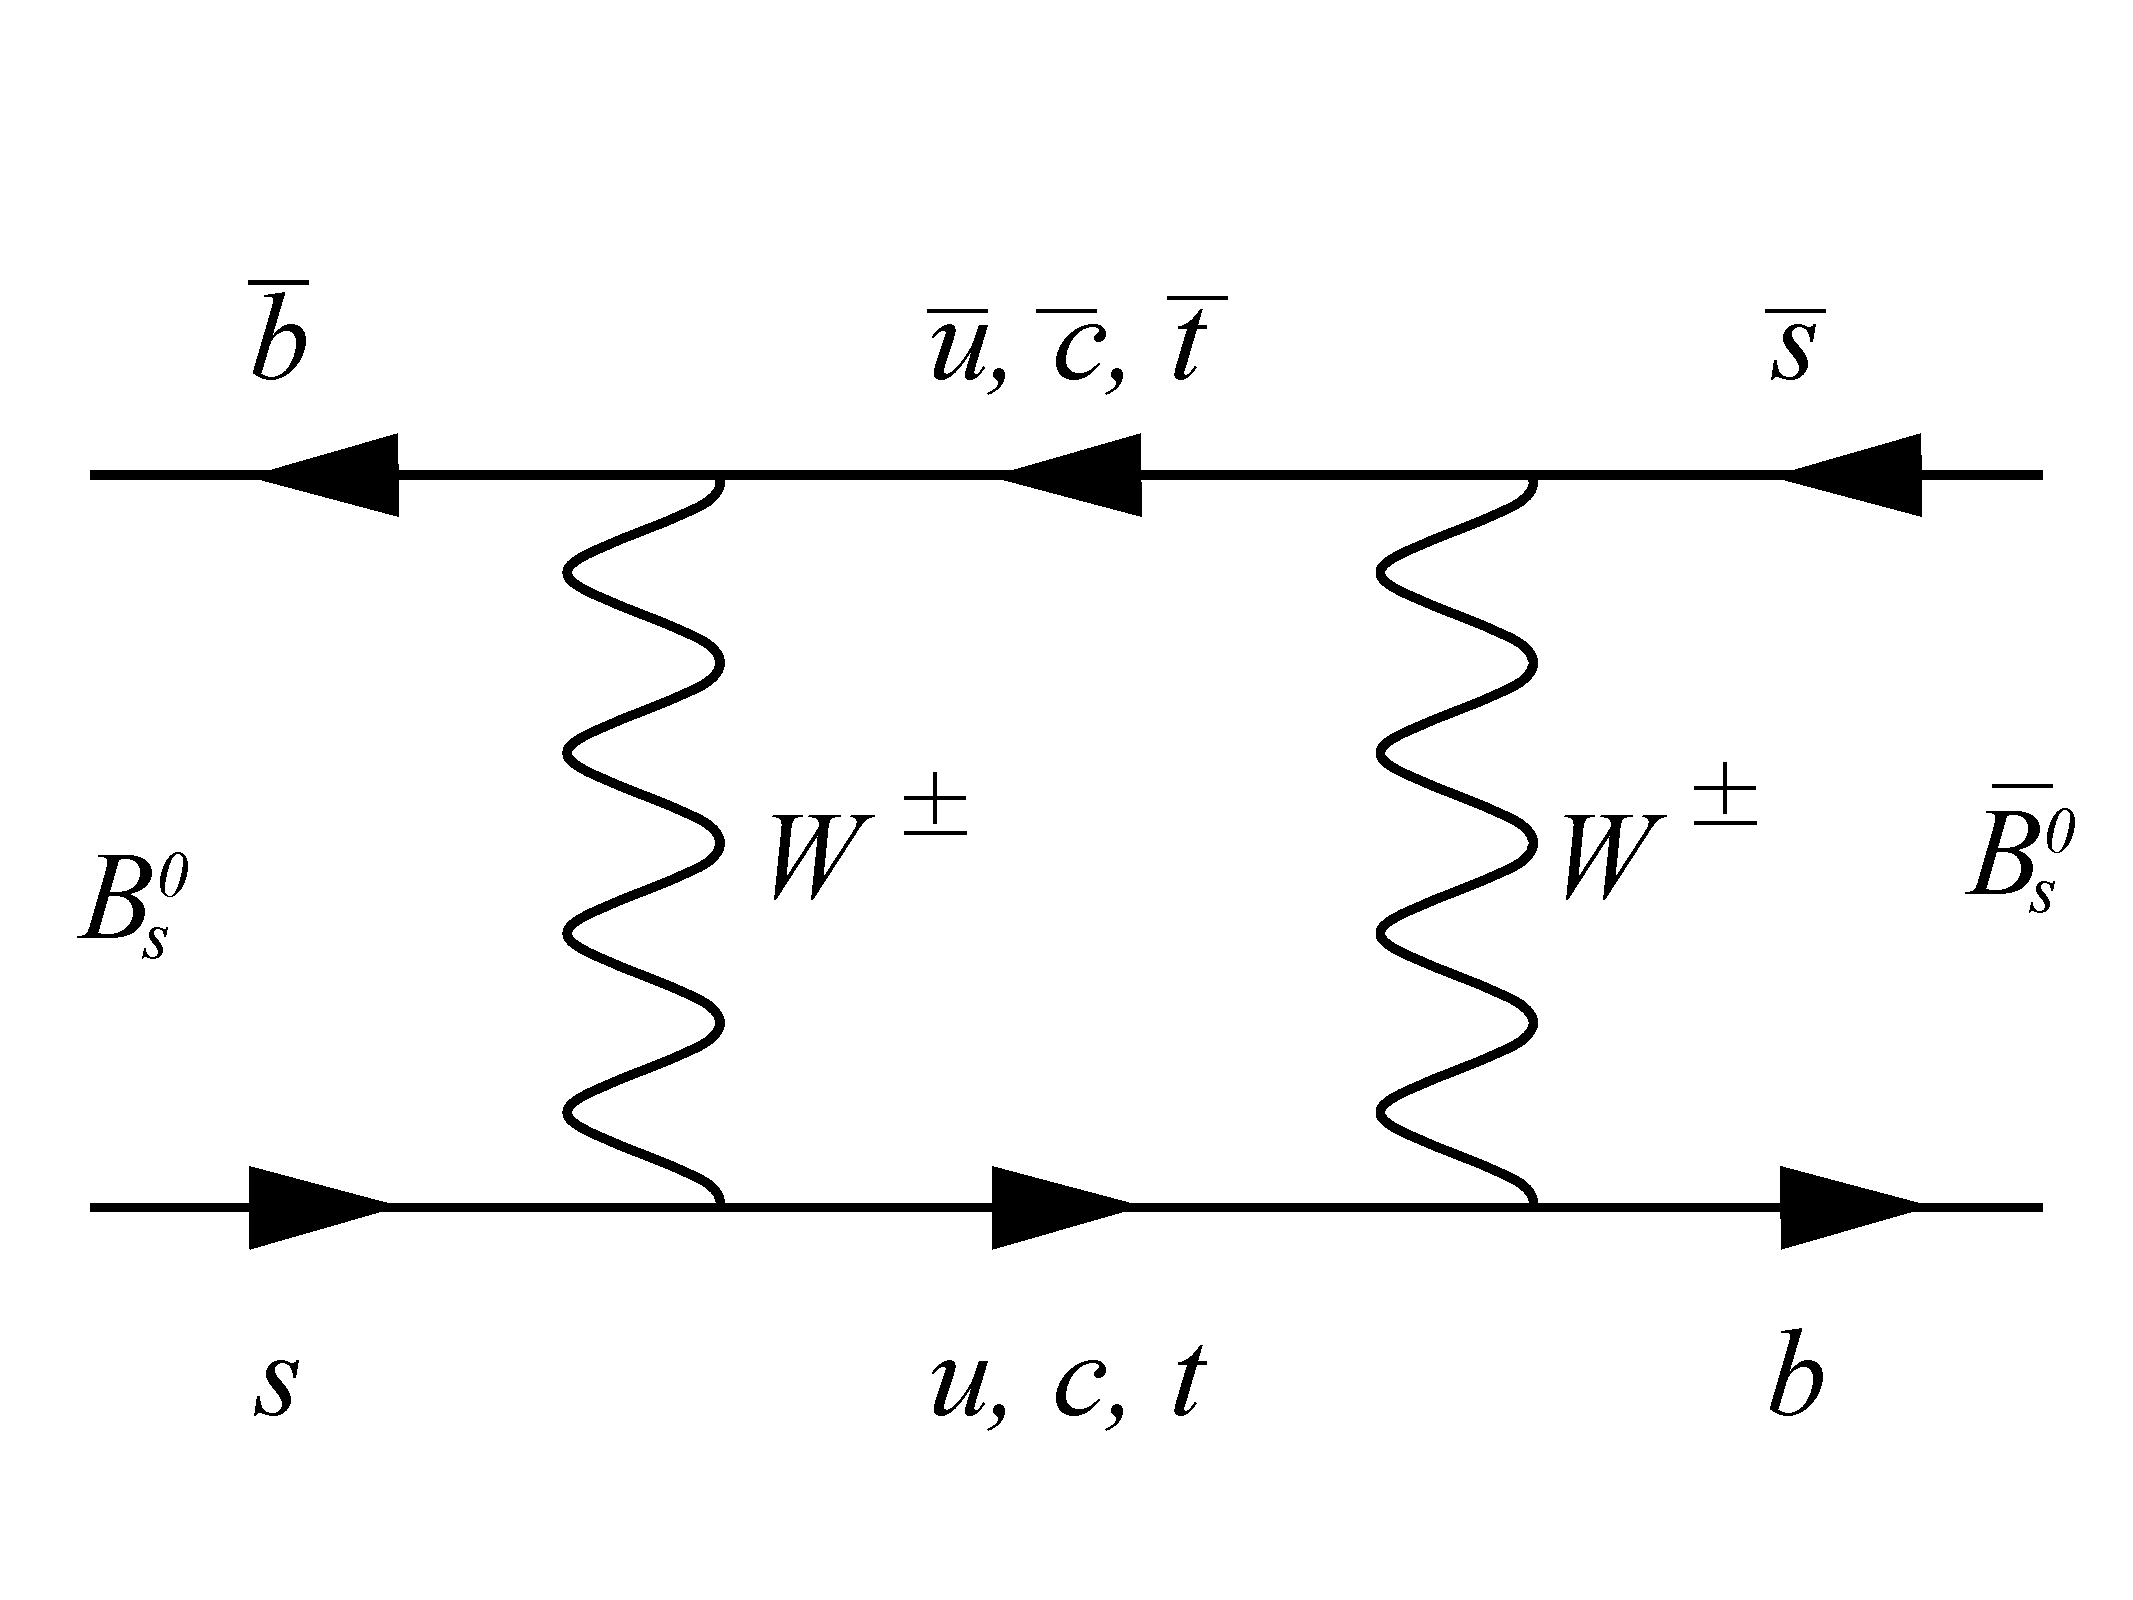
\includegraphics[width=0.5\textwidth]{./Figs/Theory/Oscillation_2.pdf}
    \caption{Oscillation of \bs and \barbs quarks through the exchange of $W$ bosons. The same diagrams apply to \bd and \barbd oscillations but with the $s$ quark exchanged for a $d$ quark.}
    \label{fig:Oscl_diag}
\end{figure}
The \BFs are measured from data where \bsd and \barbsd decays are not separated, which is called as an untagged sample of \bmumu decays. Since a \bsd or \barbsd lives for $\sim 10^{-12}$~s before decaying the state that decays will not necessarily be the same as the one that was produced. The measured \BF is not the same as the `prompt' \BF used for the theoretical prediction, the measured value corresponds to the time integrated \BF given by~\cite{DeBruyn:2012wj}
\begin{equation}
  \mathcal{B}(B^0_{(s)} \to \mu^+ \mu^-)_{\mathrm{exp}} \equiv \frac{1}{2} \int^{\infty}_0 \langle \Gamma(B^0_{(s)}(t) \to \mu^+\mu^-) \rangle dt.
\label{eq:time_BF}
\end{equation}
Therefore for a meaningful comparison between the measured and predicted \BF values, the difference in the two definitions must be evaluated~\cite{DeBruyn:2012wk,Buras:2013uqa,DeBruyn:2012wj}.

\subsection[Time evolution of the \bsd]{Time evolution of the \boldmath{\bsd}}
\label{sec:oscillations}
Initially each $b$ and $\bar{b}$ quark hardonises to form a \bsd or \barbsd described at $t=0$ by the states $| B^0_{(s)} \rangle$ and $| \overline{B}^0_{(s)} \rangle$. In order to evaluate the time integrated \BFs the evolution of these states with time must be evaluated. The time dependant Schr\"{o}dinger equation (TDSE) describes the time evolution of the particle and anti-particle states as
\begin{equation}
i \frac{d}{dt}\begin{pmatrix}{| B^0_{(s)}(t) \rangle \\ | \overline{B}^0_{(s)}(t) \rangle }\end{pmatrix} = \Bigg{(} \mathbf{M} - \frac{i\mathbf{\Gamma}}{2} \Bigg{)} \begin{pmatrix}{| B^0_{(s)}(t) \rangle \\ | \overline{B}^0_{(s)}(t) \rangle }\end{pmatrix}. 
\label{eq:TDSE}
\end{equation}
$\mathbf{M}$ and $\mathbf{\Gamma}$ are $2 \times 2$ hermitian matrices describing mass and decay time with the properties $M_{12}^{*} = M_{21}$ and $\Gamma_{12}^{*} = \Gamma_{21}$. Invariance under charge, parity and time inversion introduces additional constraints of $M_{11} = M_{22}$ and $\Gamma_{11} = \Gamma_{22}$. 

The \bsd-\barbsd oscillations ensure that for any $t>0$ the particles are a superposition of $| B^0_{(s)} \rangle$ and $| \overline{B}^0_{(s)} \rangle$ states. The off diagonal elements in the mass and decay time matrices mean that the eigenstates of the TDSE have different masses and lifetime to the \bsd and \barbsd. The eigenstates can be given by heavy, $H$, and light, $L$, mass states defined at $t=0$ as
\begin{equation}
| B_H \rangle = p | B^0_{(s)} \rangle - q |\overline{B}^0_{(s)} \rangle, \qquad |B_L \rangle = p  | B^0_{(s)} \rangle + q \overline{B}^0_{(s)} \rangle
\label{eq:mass_states}
\end{equation}
with eigenvalues of $(m_{H,L} - i\Gamma_{H,L}/2)$ and the coefficients $p$ and $q$ are constrained by $|p|^2 + |q|^2 = 1$. The eigenvalues are different for the \bd and \bs systems however the treatment of the two systems is identical, to simplify the notation only the \bs system will be described in the following discussion.
The time evolution of the heavy and light mass eigenstates is given by
\begin{equation}
  | B_H (t)\rangle = | B_H \rangle e^{-i(m_H - i\frac{\Gamma_H}{2})t}, \qquad | B_L (t)\rangle = | B_L \rangle e^{-i(m_L - i\frac{\Gamma_L}{2})t}
\label{eq:time1}
\end{equation}
from the TDSE. Therefore the time evolution of the flavour states can now be determined from equations~\ref{eq:mass_states} and~\ref{eq:time1} as
\begin{align}
| B^{0}_{s}(t) \rangle &= \frac{1}{2p}\left(|B_{L}(t)\rangle + |B_{H}(t) \rangle \right)  = f_{+}(t) |B^{0}_{s} \rangle + \frac{q}{p}f_{-}(t) |\overline{B}^{0}_{s}\rangle \\
| \overline{B}^{0}_{s}(t) \rangle &= \frac{1}{2q}\left(|B_{L}(t)\rangle - |B_{H}(t) \rangle \right)  = \frac{p}{q}f_{-}(t) |B^{0}_{s} \rangle+ f_{+}(t) |\overline{B}^{0}_{s}\rangle 
\end{align}

%\begin{align}
%\left| B^{0}_{s}(t)} \right \rangle &= \frac{1}{2p}(| B_{L} (t)\rangle  + | B_{H{ (t)\rangle) \nonumber \\
%&= f_{+}(t) | B^{0}_{(s)} \rangle  + \frac{q}{p} f_{-}(t)\overline{B}^{0{_{(s)} \rangle \\
%\left| \overline{B}^{0}_{s}(t) \right\rangle &= \frac{1}{2q}(| B_{L} (t)\rangle -  | B_{H} (t)\rangle) \nonumber \\
%&= \frac{p}{q}f_{-}(t)| B^{0}_{s} \rangle  + f_{+}(t)\overline{B}^{0}_{s} \rangle 
%\end{align}
where 
\begin{equation}
f_{\pm} = \frac{1}{2} e^{-i(m_s - i\Gamma_s)t} \left \{ e^{i(\Delta m_s + i \Delat\Gamma_s)t/2} \pm e^{-i(\Delta m_s + i \Delat\Gamma_s)t/2} \right \}.
\end{equation}
The relationships
\begin{align}
m_s &\equiv \frac{m_H + m_L}{2}, &  \Delta m_s &\equiv m_H - m_L,\\
\Gamma_s &\equiv \frac{(\Gamma_H + \Gamma_L)}{2}, & \qquad \Delta \Gamma_s &\equiv \Gamma_L - \Gamma_H,
\label{eq:deltas}
\end{align}
have been used in the expressions of $|B^{0}_{s}(t)\rangle$ and $|\overline{B}^{0}_{s} \rangle$. The difference $\Delta m_s$ is defined so that it is always positive whereas $\Delta\Gamma_s$ can take either sign. The time evolution is written in terms of these variables because $\Delta m_s$ and $\Delta\Gamma_s$ are measurable quantities.

Theoretical predictions can be calculated for $M_{12}$ and $\Gamma_{12}$ therefore it is useful to express the measurable quantities in terms of them. This is done by solving the characteristic equation of the TDSE, $|\mathbf{M} - i \mathbf{\Gamma}/2 - \lambda \mathbf{I}| = 0$, which has the solutions
\begin{equation}
\Delta m^2 - \frac{\Delta\Gamma^2}{4} = 4(|M_{12}|^2 - \frac{1}{4} |\Gamma_{12}|^2) 
\end{equation}
\begin{equation}
\Delta m \Delta \Gamma = 4 |\Gamma_{12}| |M_{12}| \cos \phi
\end{equation}
where $\phi \equiv \mathrm{arg}(-M_{12}/\Gamma_{12})$.

The observed relationship $\Delta \Gamma \ll \Delta m$ as well as $\Gamma_{12} \ll M_{12}$~\cite{Nierste:2009wg} are used to separate the expressions for $\Delta m$ and $\Delta \Gamma$ to give
\begin{equation}
\Delta m = 2 |M_{12}| \left( 1 + \mathcal{O}\left ( \left | \frac{\Gamma_{12}}{M_{12}} \right |^2 \right) \right) 
\end{equation}
\begin{equation}
\Delta \Gamma = 2|\Gamma_{12}|\cos \phi  \left(1 + \mathcal{O} \left ( \left | \frac{\Gamma_{12}}{M_{12}} \right |^2 \right ) \right)
\end{equation}
The values of $p$ and $q$ can also be related to the measurable quantities and $\Gamma_{12}$ and $M_{12}$ by diagonalising $(\mathbf{M} - \frac{i}{2}\mathbf{\Gamma})$ to produce
\begin{align}
\frac{q}{p} &= -\frac{\Delta m_{s}^{2} + i \Delta \Gamma_{s}/2 }{2M_{12} - i \Gamma_{12}} \approx - e^{-i\phi_{M}}\left (1-\frac{a}{2} \right ) + \mathcal{O}\left ( \left | \frac{\Gamma_{12}}{M_{12}} \right |^{2} \right ) 
\end{align}
where $\phi_M \equiv \mathrm{arg}(M_{12}/|M_{12}|)$ and $ a \equiv |\Gamma_{12}}/M_{12}|}\sin \phi$ and the relationships $\Delta \Gamma \ll \Delta m$ and $\Gamma_{12} \ll M_{12}$ have been used. The value of $\phi_M$ is related to the elements of the CKM matrix and $\phi_M = \mathrm{arg}(V_{tb}^*V_{td})$ for the \bd and $\phi_M = \mathrm{arg}(V_{tb}^*V_{ts})$ for the \bs. The ratio of $p$ and $q$ is given in terms of the small parameter $a$ which is needed to evaluate some SM processes. 

The necessary parameters used to describe the time evolution of \bsd and \barbsd states have now been expressed in terms of measurable or predictable quantities therefore the time dependant decay rates can now be evaluated. The decay rates can be expressed as
\begin{align}
\Gamma (B^0_{(s)}(t) \to \mu^+ \mu^-) = \mathcal{N}|\langle \mu \mu | B^0_{(s)} \rangle|^2, \quad
\Gamma (\overline{B}^0_{(s)}(t) \to \mu^+ \mu^-) =\mathcal{N}|\langle \mu\mu | \overline{B}^0_{(s)} \rangle|^2
\end{align}
where $\mathcal{N}$ encompasses the additional terms in Equation~\ref{sec:FGR} from kinematic parameters. For the evaluation of the time dependant decay rates, the exact form of the transition amplitude is not needed. A new parameters is defined
\begin{equation}
\lambda_{\mu\mu} = \frac{q}{p} \left| \frac{\overline{A}_{\mu\mu}}{A_{\mu\mu}}\right|
\end{equation}
where $A_{\mu\mu} = \langle \mu^+\mu^- | B^0_s \rangle$ and $\overline{A}_{\mu\mu} = \langle \mu^+\mu^- |\overline{B}^0_s \rangle$ to simplify the decay rate expression. Combining the information in Equations~\ref{} and using $\lambda_{\mu\mu}$ the time dependant decay rates are
\begin{align}
\Gamma(B^0_s(t) \to \mu^+ \mu^-) &=  \frac{1}{2} \mathcal{N} |A_{\mu\mu}|^2 e^{- \Gamma_s t} \bigg\{ (1 + |\lambda_{\mu\mu}|^2) \cosh \left( \frac{\Delta \Gamma_s t}{2} \right) + ( 1 - |\lambda_{\mu\mu}|^2) \cos(\Delta m_s t) \nonumber \\
& \quad {}- 2\mathrm{Re}(\lambda_{\mu\mu})\sinh \left(\frac{\Delta \Gamma_s t}{2}\right) - 2\mathrm{Im}(\lambda_{\mu\mu})\sin(\Delta m_s t) \bigg\} \label{eq:decayratesApart}\\
\Gamma(\overline{B}^0_s(t) \to \mu^+ \mu^-) &=  \frac{1}{2} \mathcal{N} (1 + a)|A_{\mu\mu}|^2 e^{- \Gamma_s t} \bigg\{ (1 + |\lambda_{\mu\mu}|^2) \cosh \left( \frac{\Delta \Gamma_s t}{2} \right) \nonumber \\
& \quad {}- ( 1 - |\lambda_{\mu\mu}|^2) \cos(\Delta m_s t) -2\mathrm{Re}(\lambda_{\mu\mu})\sinh \left(\frac{\Delta \Gamma_s t}{2}\right) \nonumber\\ 
& \quad {}+ 2\mathrm{Im}(\lambda_{\mu\mu})\sin(\Delta m_s t) \bigg\} \label{eq:decayratesA}
\end{align}
The time integrated \BF depends on the sum of the \bsd and \barbsd time dependant decay rates, using Equation~\ref{eq:decayratesA} and ignoring terms $\mathcal{O}(a)$ the total decay rate is
\begin{equation}
\langle \Gamma (B^0_s(t) \to \mu^+ \mu^-) \rangle & = \mathcal{N} |A_{\mu\mu}|^2 (1 + |\lambda_{\mu\mu}|^2) e^{- \Gamma_s t} \left(\cosh \left( \frac{\Delta \Gamma_s t}{2} \right) + A_{\Delta\Gamma}\sinh \left(\frac{\Delta \Gamma_s t}{2}\right)\right). 
\label{sec:decayratesB}
\end{equation}
A new parameter, $A_{\Delta \Gamma}$, has been introduced into the total decay rate and it is defined as
\begin{equation}
A_{\Delta\Gamma} = \frac{2\mathrm{Re}(\lambda_{\mu\mu})}{1 + |\lambda_{\mu\mu}|^2}.
\label{eq:A_DGa}
\end{equation}
The meaning of $A_{\Delta\Gamma}$ can be seen when the total decay rate is written in terms of the heavy and light \bsd mass eigenstates as
\begin{align}
  \langle\Gamma (B^0_s(t) \to \mu^+ \mu^-) \rangle &= \mathcal{N} |A_{\mu\mu}|^2 (1 + |\lambda_{\mu\mu}|^2) \left( (1 - A_{\Delta\Gamma})e^{-\Gamma_L t} + (1 + A_{\Delta\Gamma})e^{-\Gamma_{H} t} \right) \nonumber \\
&= R_H e^{-\Gamma_H t} + R_L e^{-\Gamma_L t}
\label{eq:decayratesC}
\end{align}
The final expression for the decay rates shows how \bmumu decays can be described in terms of the sum of the decays of the heavy and light mass eigenstates. The parameter \ADG is therefore related to the number of heavy and light mass eigenstates that decay as
\begin{equation}
A_{\Delta\Gamma} = \frac{R_H - R_L}{R_H + R_L}.
\end{equation}
The values \ADG can take range from +1 when only heavy mass eigenstates decay as \bsmumu and $-1$ when only light mass eigenstates decay as \bsmumu.
\subsection{Impact on the Branching Fraction}
\label{sec:BFimpact}
The time dependant decay rates are used to understand the difference between the two \BF definitions. The final form of the decay rates in Equation~\ref{eq:decayratesC} is used in the evaluations of the \BFs. The `prompt' \BF used in the theoretical predictions is
\begin{align}
\mathcal{B}(B^{0}_{s} \to \mu^{+} \mu^{-})_{\mathrm{th}} &= \frac{\tau_{B_{s}}}{2} \langle \Gamma(B^{0}_{s} \to \mu^{+} \mu^{-}) \rangle \\
&=\frac{\tau_{B_{s}}}{2} (R_{H} + R_{L}).
\end{align}
%\begin{align}
%  \mathcal{B}(B^{0}_{(s)} \to \mu^{+} \mu^{-})_{th}& &\equiv \frac{\tau_{B_{(s)}}}{2}\langle \Gamma (B^{0}_{(s)} \to \mu^{+}\mu^{-}) \rangle \bigg|_{t=0}\nonumber \\
% &= \frac{\tau_{B_{(s)}}{2} (R_{H} + R_{L})
%\end{align}
The time integrated \BF that is measured is
\begin{align}
  \mathcal{B}(B^{0}_{(s)} \to \mu^{+}\mu^{-})_{\mathrm{exp}} &= \frac{1}{2} \int^{\infty}_0 \langle \Gamma (B^{0}_{(s)} \to \mu^{+}\mu^{-}) \rangle  dt \nonumber \\
&= \frac{1}{2} \left( \frac{R_{H}}{\Gamma_{H}} + \frac{R_{L}}{\Gamma_{L}} \right) \nonumber \\
&= \frac{\tau_{B_{(s)}}}{2}(R_{H} + R_{L}) \left[ \frac{1 + A_{\Delta\Gamma}y_{(s)}}{1 - y_{(s)}^{2}} \right]
\end{align}
where $y_{(s)}$ relates the heavy and light mass eigenstate decay times as $y_{(s)} = \Delta \Gamma_{(s)} / 2\Gamma_{(s)}$. Therefore the measured and prompt \BF values are related as
\begin{equation}
  \mathcal{B}(B^0_{(s)} \to \mu^+\mu^-)_{\mathrm{exp}} = \left[ \frac{1 + A_{\Delta\Gamma}y_{(s)}}{1 - y_{(s)}^{2}} \right] \mathcal{B}(B^0_{(s)} \to \mu^+ \mu^-)_{\mathrm{th}}
\end{equation}
For the $B^0$-$\overline{B}^0$ oscillations the difference in the lifetimes of the heavy and light mass eigenstates is extremely small therefore $y$ negligible and the prompt \BF is equivalent to the experimental \BF. However for \bs-$\overline{B}^0_s$ oscillations there is a large difference in the lifetimes of the mass eigenstates and $y_s =0.062 \pm 0.006$~\cite{Amhis:2016xyh}. The prompt \BF must therefore be corrected to account for the oscillations before it is compared to the experimental value.
\section[\ADG and the effective lifetime]{\boldmath{\ADG} and the effective lifetime}
\label{sec:ADG_EL}
The definition of \ADG in Equation~\ref{eq:A_DGa} shows that it depends upon the transition amplitude of \bsmumu decays. In Section~\ref{sec:BFdef} the effective Hamiltonian for this decay was discussed and the \BF given in terms of the complex variables $P$ and $S$. Therefore \ADG can also be expressed in terms of these parameters as~\cite{DeBruyn:2012wk}
\begin{equation}
A_{\Delta \Gamma} = \frac{|P|\cos \varphi_P + |S| \cos \varphi_S}{|P|^2 + |S|^2}
\label{eq:NP_ADG}
\end{equation}
In the SM $P=1$ and $S=0$ therefore \ADG takes the maximal value of +1 and only the heavy mass eigenstate decays as \bsmumu. This can be understood because the final state of a \bsmumu decay is a $\mathcal{CP}$ odd state and the heavy \bs mass eigenstate is a $\mathcal{CP}$ odd state state.

As discussed in Section~\ref{sec:BFdef}, NP models can alter the values of $P$ and $S$, moving them away from the SM expectations. A change in these values could alter both the measured \BF and \ADG or just one of these observables. Since the comparison of the measured \BF to the SM prediction relies on \ADG, in order to understand possible NP effects in \BF, \ADG must be measured as well. 

The value of \ADG can be measured directly from the time dependant decay rate of \bsmumu decays. This method involves separating the \bsmumu decays into those with $| B^0_s \rangle$ and $|\overline{B}^0_s\rangle$ initial states, which needs a large number of \bsmumu decays. Since \bsmumu are very rare decays this approach is currently not viable. Alternatively \ADG can be measured through the \bsmumu effective lifetime~\cite{DeBruyn:2012wj}. The effective lifetime is the mean decay time of an untagged sample of \bsmumu decays, defined as~\cite{Fleischer:2011cw}
\begin{equation}
  \tau_{\mu\mu} \equiv \frac{\int^{\infty}_0 t\langle \Gamma (B^0_s \to \mu^+ \mu^-) \rangle dt}{\int^{\infty}_0 \langle \Gamma (B^0_s \to\mu^+ \mu^-) \rangle dt}.
\label{eq:EL_def}
\end{equation}
It can be measured by fitting a single exponential to the same set of decays used to measure the \BF~\cite{DeBruyn:2012wj}. The effective lifetime can be expressed in terms of \ADG using the decay rates in Equation~\ref{eq:decayratesC} as
\begin{align}
\tau_{\mu\mu} %&=\frac{\frac{R_{H}}{\Gamma_{H}^{2}} + \frac{R_{L}}{\Gamma_{L}^{2}}}{\frac{R_{H}}{\Gamma_{H}^{2}} + \frac{R_{L}}{\Gamma_{L}}}  \nonumber \\
= \frac{\tau_{B_{s}}}{(1 - y_{s}^{2})} \frac{( 1 + 2A_{\Delta\Gamma}y_{s} + y_{s}^{2})}{(1 + A_{\Delta\Gamma}y_{s})}.
\end{align}
%\begin{align}
%\tau_{\mu\mu} &= \frac{\frac{R_{H}}{\Gamma_{H}^{2}} + \frac{R_{L}}{\Gamma_{L}^{2}}}{\frac{R_{H}}{\Gamma_{H}} + \frac{R_{L}}{\Gamma_{L}}}\\
%&=  \frac{\tau_{B_{s}}}{(1 - y_{s}^{2}) \frac{(1 + 2 A_{\Delta\Gamma}y_{s} + y_{s}^{2})}{(1 + A_{\Delta\Gamma}y_{s})}
%\label{eq:EL_ADG}
%\end{align}
In the SM only the heavy \bs mass eigenstates decays as \bsmumu and the \el equals the lifetime of the heavy mass eigenstate, $\tau_{\mu\mu} = \tau_H = \frac{1}{\Gamma_H}$. The effective lifetime offers a measurement complementary to the \BFs to study the SM and NP models in \bsmumu decays due to the dependant of the \el on \ADG.

\section{The Standard Model predictions}
\label{sec:SM_predictions}

The SM provides precise predictions of the \bmumu \BFs of~\cite{Bobeth:2013uxa, Aoki:2016frl, Fleischer:2017ltw}
\begin{align}
\mathcal{B}(B^0_{s} \to \mu^+ \mu^-)& = (3.57 \pm 0.16) \times 10^{-9}\\
\mathcal{B}(B^0 \to\mu^+ \mu^-)& = (1.02 \pm 0.06) \times 10^{-10}
\end{align}
where quark oscillations have been accounted for in the quoted value of the \bsmumu \BF. The largest contributions to the theoretical uncertainties come from the CKM matrix elements and the decay constants of the \bs and the \bd.
The ratio of the \BF values, defined in Equation~\ref{eq:BF_ratio} is~\cite{CMS:2014xfa} 
\begin{equation}
\mathcal{R} = \frac{\mathcal{B}(B^0 \to\mu^+ \mu^-)}{\mathcal{B}(B^0_{s} \to \mu^+ \mu^-)} = 0.0295^{+0.0028}_{-0.0025}.
\end{equation}
In the SM the \bsmumu effective lifetime is predicted to be~\cite{Fleischer:2017ltw}
\begin{equation}
\tau_{\mu\mu} = 1.61 \pm 0.01 \mathrm{ps}.
\end{equation}
The Heavy Flavour Averaging group provides the world averages for the measured values of the lifetime of the light and heavy \bs mass eigenstates to be $\tau_{H} = 1.609 \pm 0.010$~ps and $\tau_{L} = 1.414 \pm 0.006$~ps~\cite{Amhis:2016xyh}.
The difference in these lifetimes is $0.195$~ps.
Therefore a precision of 0.38~ps would be needed to distinguish between \ADG = $+1$ and \ADG = $-1$ a 5$\sigma$ with the \el. 



\section{New Physics models and \bmumu decays}
\label{sec:NPmodels}
There exist a large number of BSM theories that can influence \bmumu decays in different ways. Measurements of the \bmumu \BFs and \bsmumu effective lifetime can constrain the parameter space available for NP and could reveal which theories are the correct extension of the SM. This section will briefly introduce how some NP models that could still be seen with \bmumu decays given the current precision of the \BF measurements. %can be studied with \bmumu decays.
For a more detailed discussions of NP models relevant to \bmumu decays and contraints on these models from measurements see references~\cite{Buras:2013uqa,Knegjens:2014zva,Altmannshofer:2014rta}.

As discussed in Section~\ref{sec:BFdef} the ratio of the \bdmumu and \bsmumu \Bfs provides an excellent test of the flavour structure of the SM and BSM theories. %Both the measured ratio and theoretical predictions are more precise than the individual \BFs due to the cancellation of uncertainties in the ratio. 
Figure~\ref{fig:ratio} shows possible values accessible by BSM theories alongside the SM prediction. The prediction of the Minimal Flavour Violation (MFV)~\cite{DAmbrosio:2002vsn} hypothesis is included in Figure~\ref{fig:ratio}. 
\begin{figure}[htbp]
    \centering
        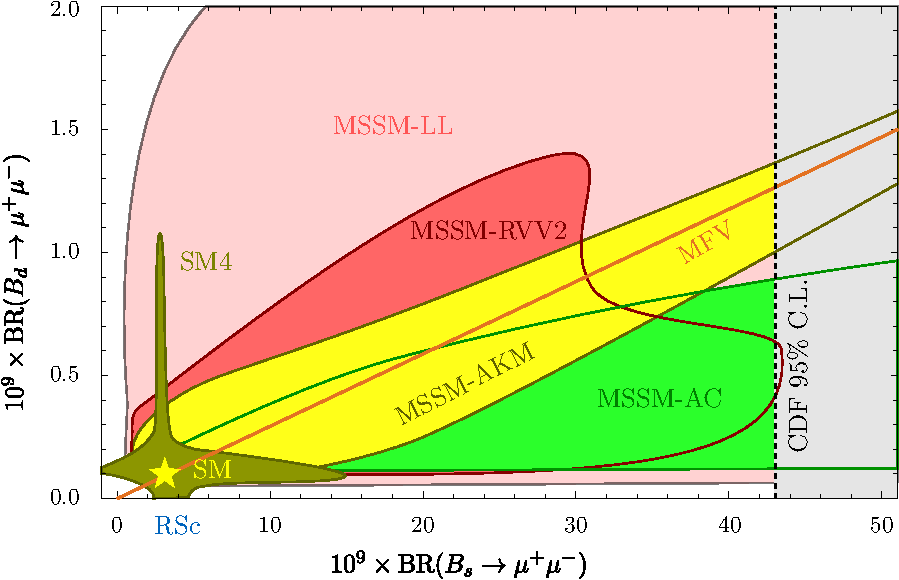
\includegraphics[width=0.8\textwidth]{./Figs/Theory/MFV.pdf}
    \caption{Correlations between the \bdmumu and \bsmumu \BFs including the SM prediction, the Minimal Flavour Violation hypothesis (MFV), four Minimal Supersymmetric Standard Models (MSSM)~\cite{Martin:1997ns} and the SM extended to constrain four generations of fermions~(SM4)~\cite{Hou:2008xd}. Figure is taken from~\cite{Straub:2010ih}.}
    \label{fig:ratio}
\end{figure}
The MFV hypothesis predicts that the coupling of quark flavour and $\mathcal{CP}$ violation follow the same Yukawa structure as the SM in NP models. It is a popular theory to describe the flavour structure in NP models due to the current agreement of measurements with the SM predictions. A significant deviation of the \BF ratio from the SM or MFV hypothesis predictions would indicate the need to a new flavour structure in theoretical models.

Additionally NP models could move the \BFs and \ADG away from the SM predictions by providing new particles that can contribute to the decays. These new particles would change the Wilson coefficients included in the parameters $P$ and $S$. The dependence of the \BFs and \ADG on $P$ and $S$ are different, as shown in Equations~\ref{eq:BF_form} and~\ref{eq:NP_ADG}, therefore NP models can influence the observables independently. The allowed values of \ADG and the ratio of the measured \BF to prompt SM prediction are shown in Figure~\ref{fig:NPmodelsB} for possible situations where $S=0$, $P=1$, $P\pm S = 1$ and $\varphi_P, \varphi_S \in {0, \pi}$. These figures illustrate that if NP effects are not revealed in the \BF measurements, they could still appear in \ADG. Furthermore in some scenarios \ADG is needed to resolve degeneracies that arise from information from the \BF alone.
\begin{figure}[tbp]
    \centering
        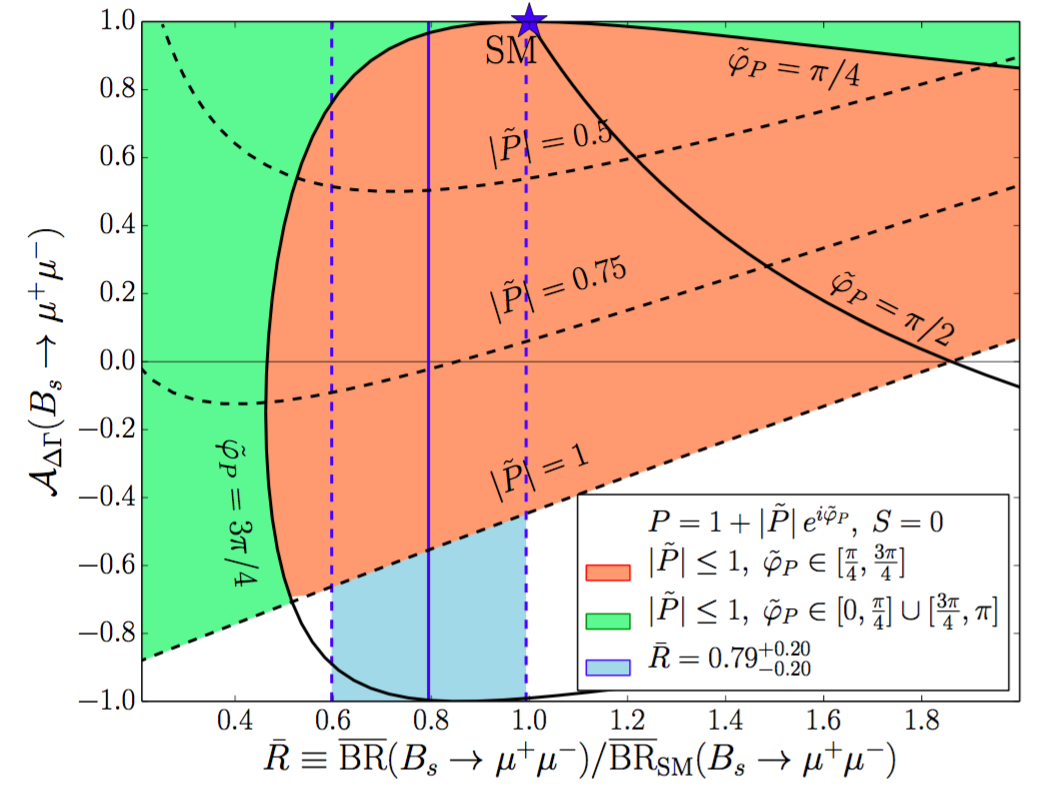
\includegraphics[width=0.49\textwidth]{./Figs/Theory/NP_S_0.png}
        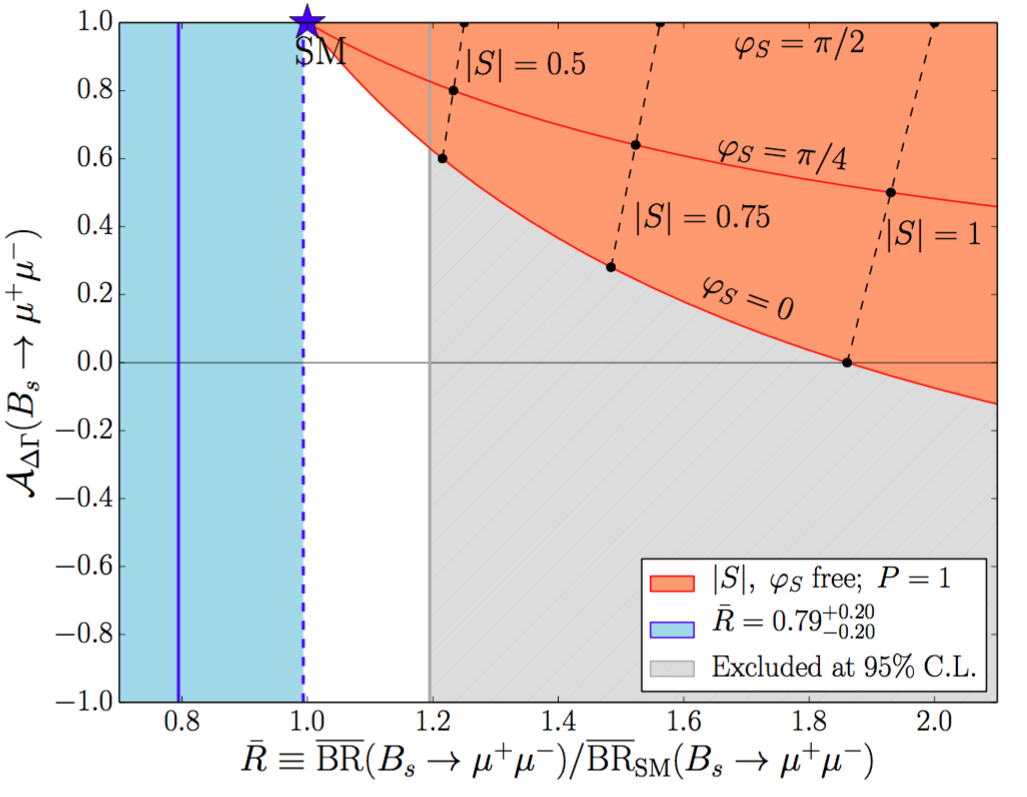
\includegraphics[width=0.49\textwidth]{./Figs/Theory/NP_P_1.png}
        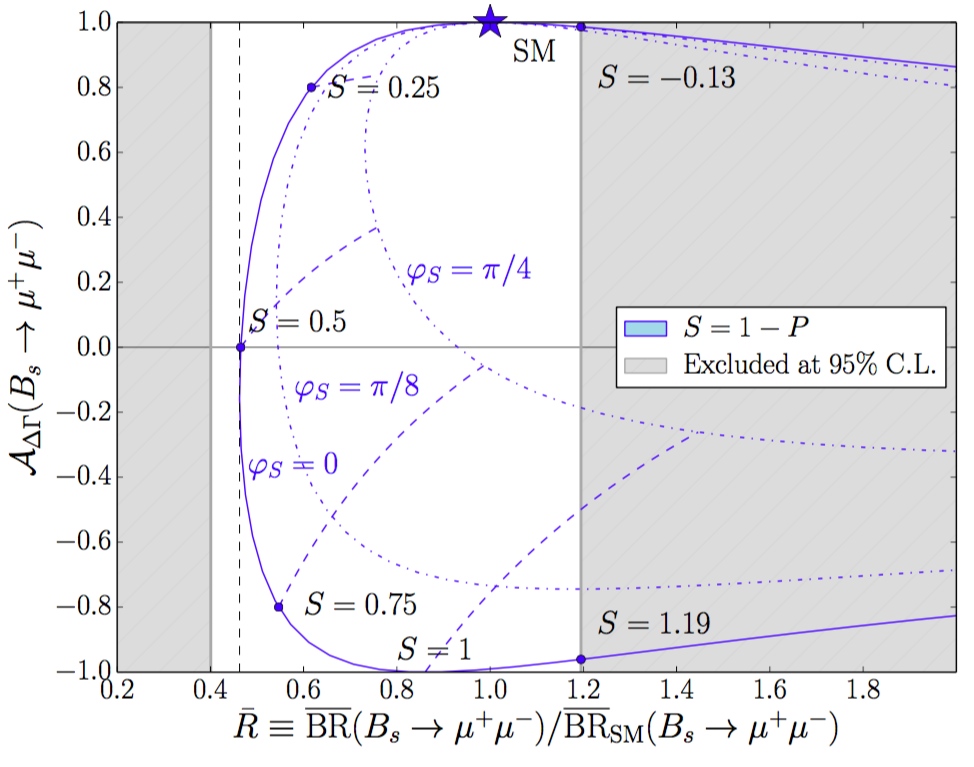
\includegraphics[width=0.49\textwidth]{./Figs/Theory/NP_P_pm_S_1.png}        
        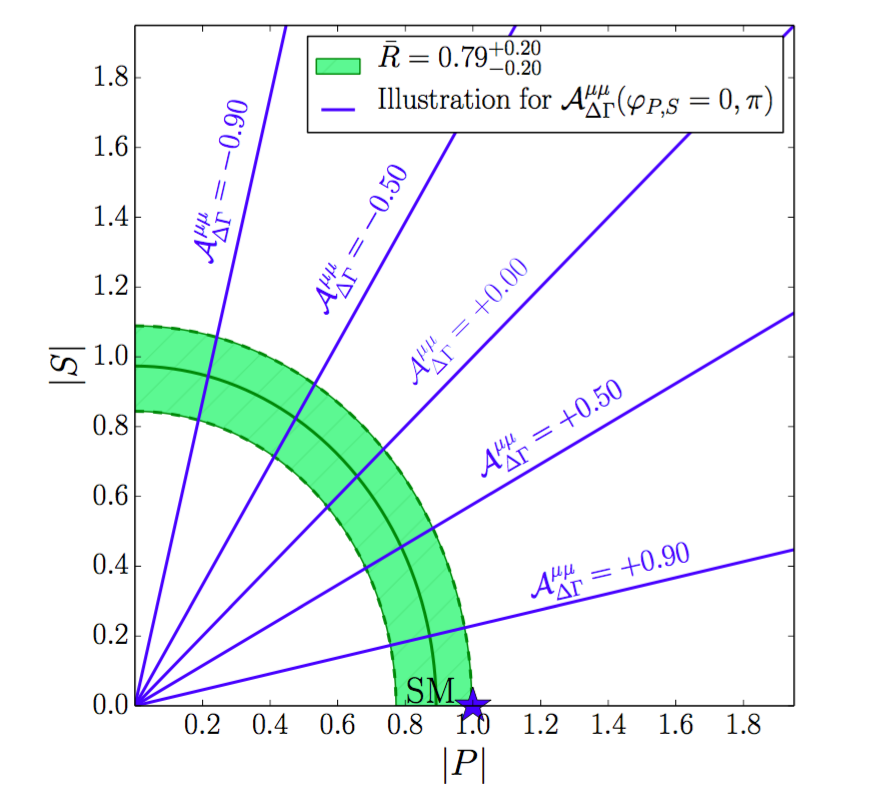
\includegraphics[width=0.45\textwidth]{./Figs/Theory/NP_phi.png}
    \caption{Allowed values for $\mathcal{B}$(\bsmumu) and \ADG for situations where $S=0$ (top left), $P=1$ (top right), $P \pm S = 1$ (bottom left) and $\varphi_P, \varphi_S \in {0, \pi}$ (bottom right)~\cite{Buras:2013uqa,Knegjens:2014zva}. The ratio $\overline{R}$ plotted is from an average of the individual results from the CMS and LHCb collaborations from~\cite{CMSandLHCbCollaborations:2013pla}, the results from the combined analysis of the CMS and LHCb data gives $\overline{R} = 0.76^{+0.2}_{-0.18}$~\cite{CMS:2014xfa}.}
    \label{fig:NPmodelsB}
\end{figure}

Amongst the BSM theories that can influence the values of $P$ and $S$ are the two Higgs doublet model (2HDM)~\cite{HALL1981397}, supersymmetric models~\cite{Witten:1981nf}, models including leptoquarks and models that obey the MFV hypothesis as mentioned earlier.

The 2HDM extends the Higgs sector of the SM by introducing two complex scalar field doublets both with non-zero vacuum expectation values. Spontaneous symmetry breaking then produces 2 charged, one neutral pseudoscalar and 2 neutral scalar Higgs bosons. The new particles can enter the loops of \bmumu decays and allow FCNCs to occur that the tree level. Different scenarios of this model depend on the Higgs-quark interactions and can incorporate the MFV hypothesis. This model can produce scenarios where $S=0$, $P=1$ or $P\pm S = 1$~\cite{Buras:2013uqa,Knegjens:2014zva} and the corresponding \BF and \ADG values for \bsmumu decays as shown in Figure~\ref{fig:NPmodelsB}.

Supersymmetric (SUSY) models extend the SM by giving each SM particle a supersymmetric partner. The resulting theory is symmetric under the transformation of fermions to boson and bosons to fermions. So far no evidence for SUSY particles has been found therefore the symmetry must be broken and the mass of SUSY particles is greater than their SM partners. The Minimal Supersymmetric Standard Model (MSSM) includes a Higgs sector similar to the 2HDM and there are scenarios where it obeys the MFV hypothesis. \bmumu decays are sensitive to this model provided the ratio of the vacuum expectations values of the Higgs doublet is large~\cite{Babu:1999hn,Isidori:2001fv,Buras:2002vd}. The MSSM can produce values for \ADG and the \bsmumu \BF shown in Figure~\ref{fig:NPmodelsB} for situations where $P\pm S =1$ and $\varphi_P, \varphi_S \in {0, \pi}$~\cite{Buras:2013uqa,Knegjens:2014zva}.

Models including leptoquarks are currently popular to explain the anomalies observed in heavy flavour measurements~\cite{Barbieri:2016las,Becirevic:2016yqi,Hiller:2014yaa,Bauer:2015knc,Fajfer:2015ycq}. A leptoquark is a boson that carries both lepton and baryons numbers. The exact quantum numbers depend on the interactions with SM fermions and leptoquarks can enable FCNCs to occur at the tree level. Therefore leptoquarks could enhance \bmumu decays but information from \ADG is necessary for the study of leptoquarks with \bmumu decays because it resolves degeneracies that are present with just the \BF measurements~\cite{Altmannshofer:2017wqy}.

Although \bmumu decays are yet to reveal NP, the current experimental precision still leaves plenty of room for NP to be revealed. The observation of \bsmumu decays makes it possible to start investigating \ADG through the \bsmumu \el. A measurement of \ADG will proved important information, complementary to the \bmumu \BF measurements to search for NP in \bsmumu decays.

\chapter{The LHC and the LHCb experiment} 
\label{CERN_LHC_LHCb}

The European Organisation for Nuclear Research (CERN) was founded in 1954, it began with 12 member states as an organisation to encourage European collaboration and to study nuclear physics. The collaborative nature of CERN has enabled large-scale expensive experiments to be built that individual member states would not have be able to afford. The Proton Synchrotron (PS) was CERN's flagship accelerator which was operational in 1959. It had a circumference of 628~m and accelerated protons up to a center-of-mass energy of 25~\gev makig the PS highest energy particle accelerator at that time. Now 62 years since its foundation, CERN has grown to include 22 member states\footnote{Countries and organisations that are unable to become member states can still participate in scientific research as observer states \cite{Member_States}.} and is still at the forefront of high energy physics research. CERN’s latest accelerator, the Large Hadron Collider (LHC), is most energetic particle accelerator ever built, with a 27~km circumference the LHC was designed to collide protons at a centre-of-mass energy of 14~\tev. This chapter introduces the LHC and the LHC beauty experiment, one of the experiments that studies the produces of particle collisions produced at the LHC.

\section{The LHC}
\label{LHC}


The LHC is a proton synchrotron designed to accelerate and collide two beams of protons with a centre-of-mass energy of 14~\tev. Although operation of the LHC began in 2010 it is yet to reach the design energy. The purpose of the LHC is to provide high energy proton-proton $pp$ collisions, the products of which are used for precision tests of the Standard Model (SM) and to search for new physics effects that cannot be explained within the context of the SM. %particles that go beyond the scope of the SM. 
There are four interaction points on the LHC ring where the beams are brought to collide, at these points various experiments detect and study the products of particle collisions. In addition to protons, the LHC can also accelerate lead-nuclei up to 2.76~\tev per nucleon, however it is only the products from proton collisions that are studied in this dissertation.

%It's the bit below that I'm not a massive fan of the explains how the LHC gets it's protons. I think that it is a little too brief and disconnected with not explanations.
The protons accelerated by the LHC originate from hydrogen gas, %for the LHC come from hydrogen gas, %add something nice here
the hydrogen atoms are ionised to strip away the electrons and then the protons are accelerated through a chain of particle accelerators of increasing energy before being injected into the LHC. The chain of accelerators, shown in Fig.~\ref{fig:accelerator_chain}, consists of machines that were used in experiments throughout the second half of the last century and have been modified to meet the requirements needed to provide protons to the LHC. The protons leave the chain of accelerators with of energy of 450~\gev per proton and in bunches of \~$\10^{11}$ protons, as the bunches are injected into the LHC they are split into two oppositely circulating beams.
The LHC accelerates the protons to the desired centre-of-mass energy using supercooled radio frequency cavities and guides them around the ring with superconducting dipole magnets. %I could add here some details about the magnets and how the LHC accelerates the protons.                                       
Once the required energy has been reached, the bunches are focused using quadrupole magnets before being brought to collided at 4 interaction points around the LHC ring.% at a bunch crossing rate of 40~MHz.

\begin{figure}[htbp!]
  \centering
  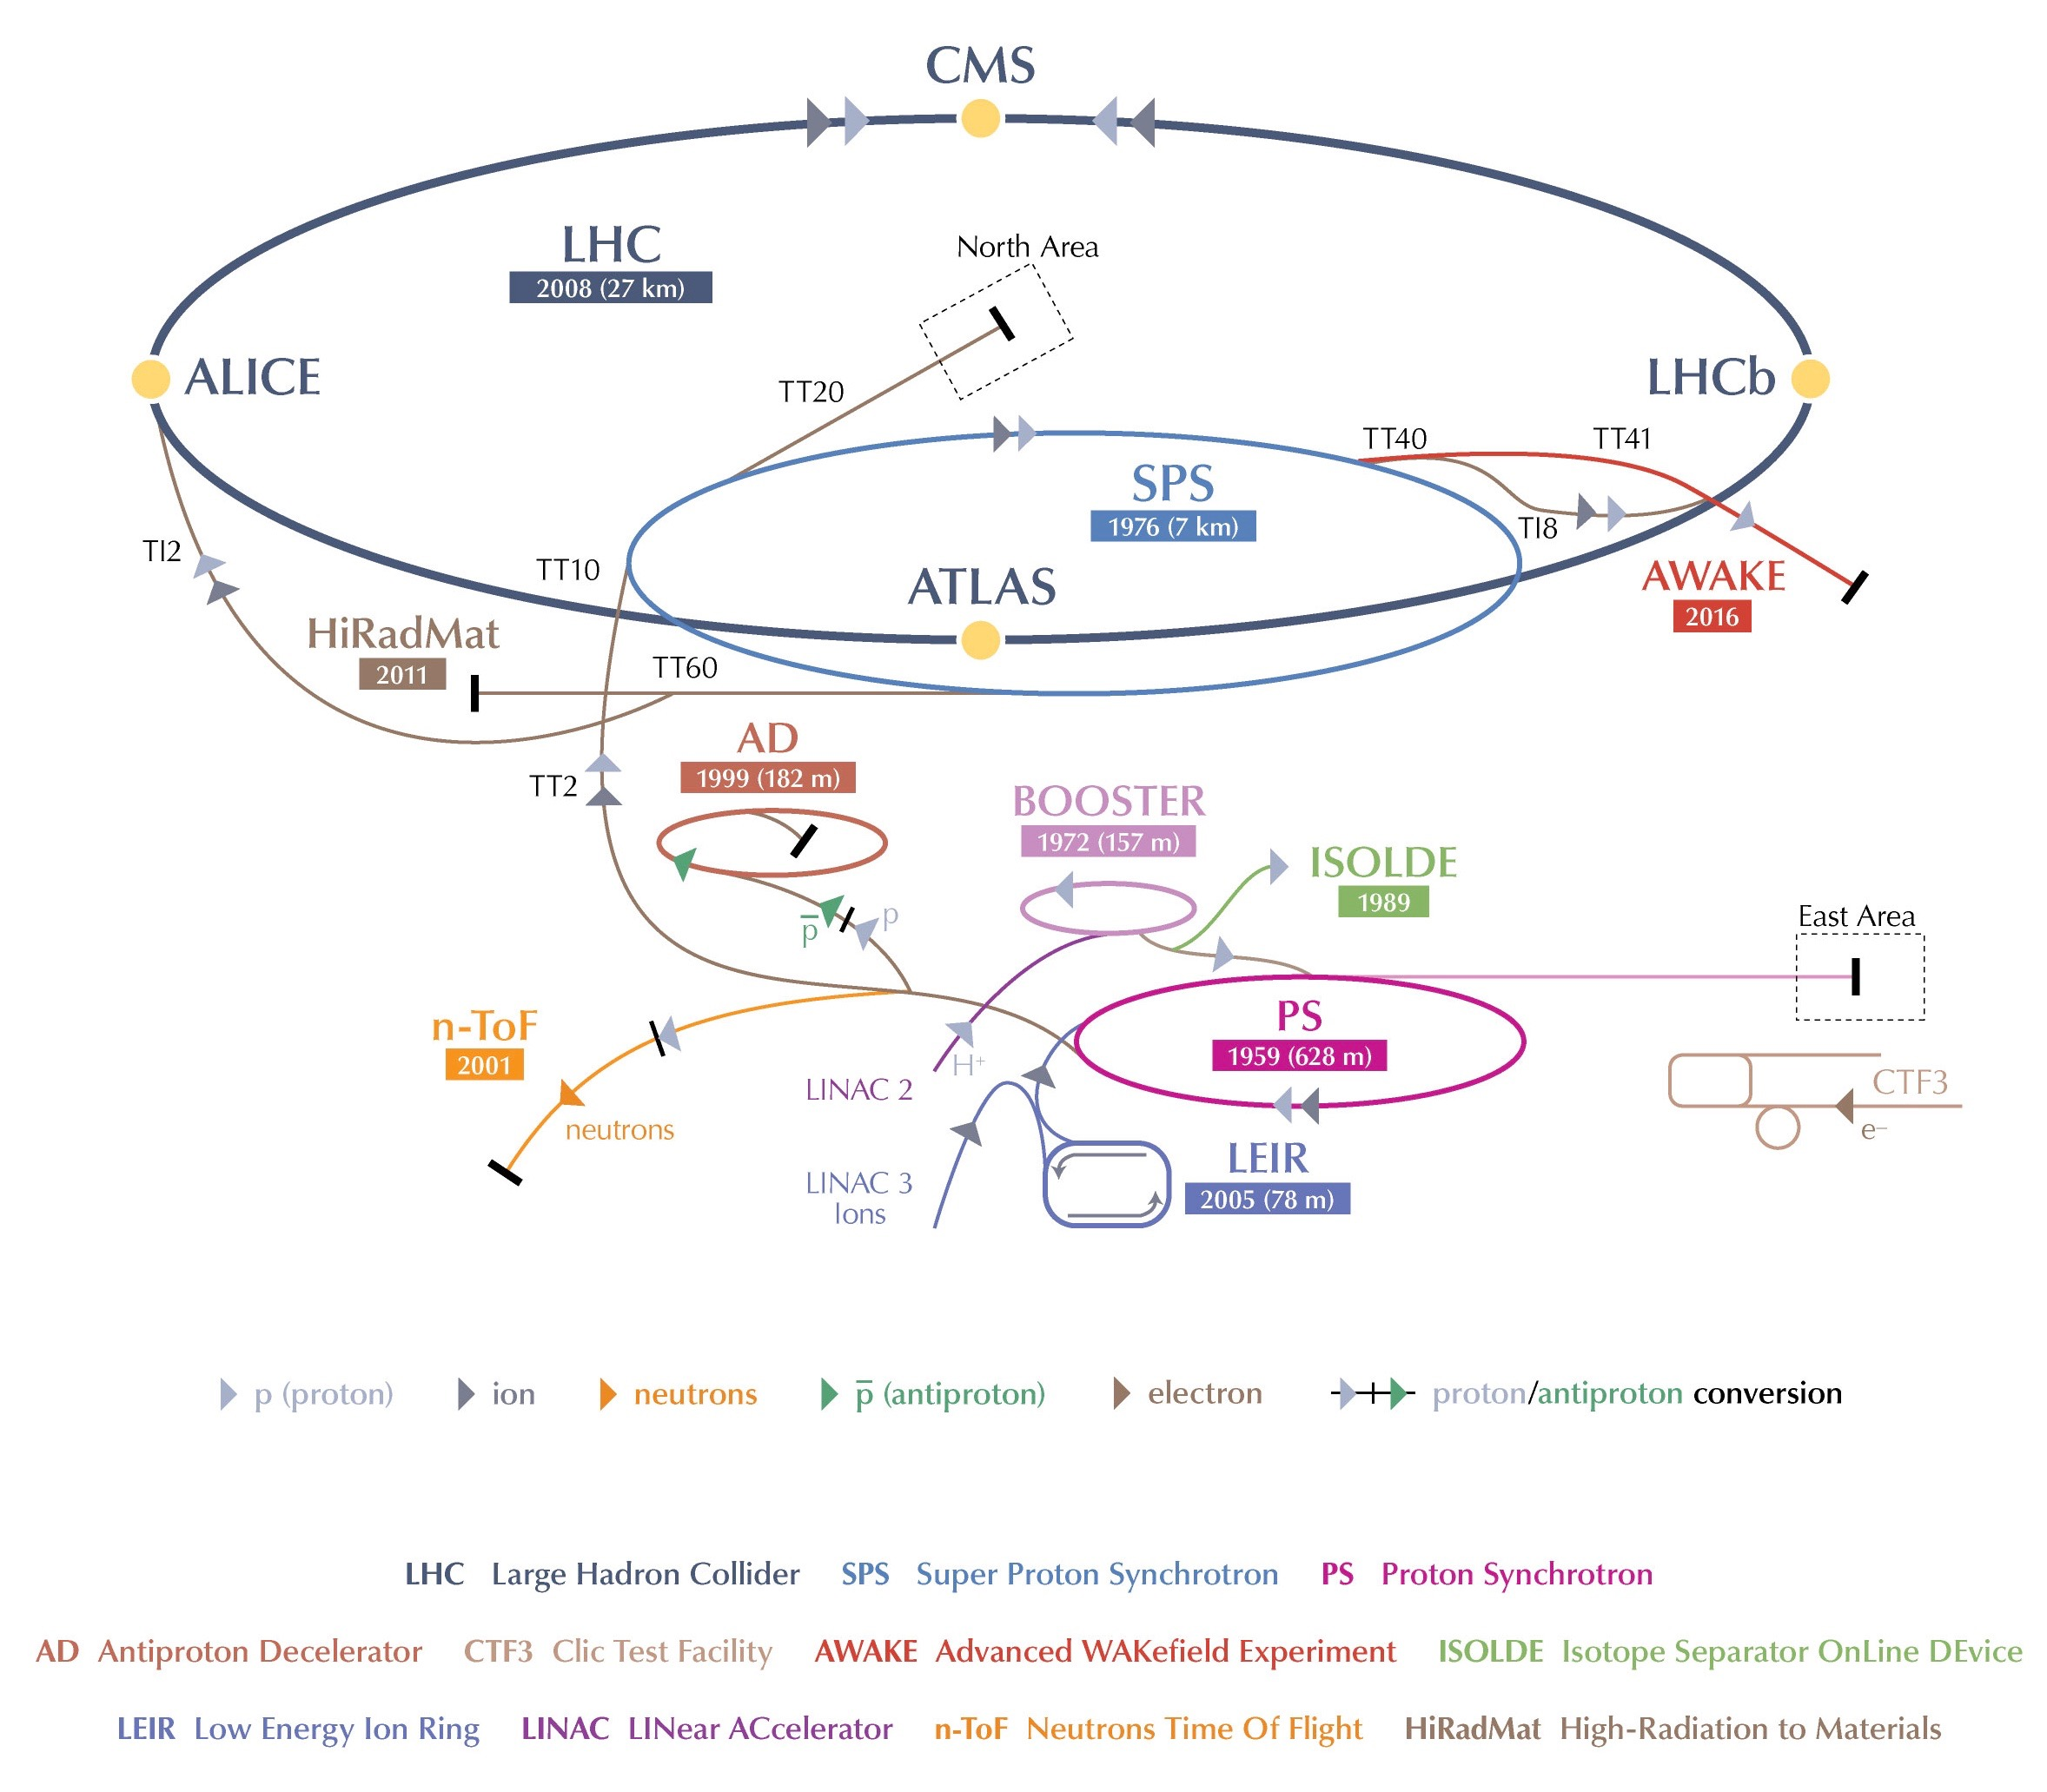
\includegraphics[trim = 125mm 2mm 125mm 90mm, clip, width=0.8\textwidth]{./Figs/LHC_LHCb/accelerator_complex.jpg}
  \caption{The accelerator complex at CERN. The chain of accelerators used to inject protons into the LHC begins with the Linac 2 which accelerates protons to 50~\mev, the protons are passed to the Proton Synchrotron Booster that accelerates them to 1.4 \gev. The Proton Synchrotron is next in the chain, accelerating protons to 25~\gev and creating the desired spacing between proton bunches. Then finally the Super Proton Synchrotron accelerating protons to 450~\gev ready for injection into the LHC. Source: CERN.}
  \label{fig:accelerator_chain}
\end{figure}



%The protons leave the chain of accelerators with of energy of 450~\gev per proton and in bunches of \~$10^{11}$ protons, as the bunches are injected into the LHC they are split into two oppositely circulating beams.
%The LHC accelerates the protons to the desired centre-of-mass energy using supercooled radio frequency cavities and guides them around the ring with superconducting dipole magnets. %I could add here some details about the magnets and how the LHC accelerates the protons.
%Once the required energy has been reached, the bunches are focused using quadrupole magnets before being brought to collided at 4 interaction points around the LHC ring.% at a bunch crossing rate of 40~MHz. 

The centre-of-mass energy of a collider is an important measure of its performance as it describes the energy avaliable to create new particules during $pp$ collisions, another important measure of collider performance is the instantaneous luminosity a collider can provide. The instantaneous luminosity, $\mathcal{L}$, is a measure of how many collisions occur per second, it is given by
\begin{equation}
\mathcal{L} = \frac{N^{2} f n_{b}}{\mathcal{F}}.
\label{eq:inst_lumi}
\end{equation}
where $N$ is the number of protons per bunch, $n_{b}$ the number of bunches per beam, $f$ the bunch revolution frequency and $\mathcal{F}$ contains information about the beam geometry. The LHC is designed to operate at a maximum instantaneous luminosity of $10^{34}$~cm$^{-2}$s$^{-1}$. To reach this luminosity the LHC can have up to 2808 proton bunches per beam with a revolution frequency of 11.245 kHz and a speration of 25 ns between each proton bunch. %, therefore the separation between proton bunches can be as short as 25~ns. 
The higher the luminosity, the more collisions happen in a second and the more particles will be produced, this can either be advantageous or disadvantageous depending on the physics process that is being studied.
% and the detector design that records the collisions. 
Therefore luminosity delivered at each interaction point can be tuned by the quadrupole magnets by altering the shape of each bunch to suit the experiments at each point.

Proton beams first circulated the LHC in 2008 and since then there have been two physics runs separated by a long shutdown period. Run 1 began in 2010 and continued until 2013, during this time protons were collided with a centre-of-mass energy of $\sqrt{s}$~=~7~TeV during 2010 and 2011, the energy was increased to $\sqrt{s}$~=8~TeV for operation during 2012. After Run~1 there was a period of long shut doen (LS1) during during work was done to prepare the LHC to operate at higher energies and renovation work was preformed on accelerators that provide the LHC with protons. Run~2 began in 2015 with proton collisions at a centre-of-mass energy of $\sqrt{s}$~=~13~TeV, %why 13TeV? I have the answer
this Run will continue until 2018 when a second period of upgrades and maintenance, the Long Shutdown~2, will begin.




There are 7 experiments on the LHC that detect particles produced in proton and heavy ion collisions. There are two general purpose detectors, ATLAS and CMS, that were designed to search for the Higgs boson and new effects that are beyond the scope of the SM, these two experiments operate at the full instantaneous luminosity of the LHC. %Perhaps say we found the Higgs?
ALICE studies quark-gluon plasma produced in heavy ion collisions to understand conditions similar to those present in the early universe. The TOTEM experiment studies properties of protons as they collide head on at the LHC and the MOEDAL experiment is aims to detect magnetic monopoles. The LHCf experiment studies particles that are thrown forward in LHC collisions to understand similar processes that occur in cosmic rays. %Finally there is the Large Hadron Collider Beauty experiment (LHCb) that will be described in the next section. %, this experiment was designed to studies rare $b$-hadron decays and $\mathcal{CP}$ violating processes and operates at a lower luminosity and has a smaller angular acceptance than the general purpose detectors. %Should probably include the full experiment names as I have done for LHCb or not include the name for LHCb.


The final experiment if the Large Hadron Collider Beauty experiment (LHCb) that will be described in the next section

\section{The LHCb experiment}
\label{LHCb}
The LHCb experiment was build to study the SM and search for new physics phenonoma through the study of $\mathcal{CP}$-violating decays and rare $b$-hadron decays. 
%The LHCb experiment was built to study CP violation and rare decays of \bhadrons to search for new physics processes that could be revealed in these decays. 
At the LHC the dominant production mechanisms of \bbbar pairs are gluon-gluon fusion, quark anti-quark annihilation and gluon-gluon splitting. The \bbbar pairs produced travel at small angles relative to the beam pipe as shown in Figure~\ref{fig:bbar_production} and hadronize to form a range of \bhadrons, including $B^{+}$, $B^{0}_{s}$ and $\Lambda^{0}_{b}$, that are studied by LHCb. 

 
\begin{figure}[tb] 
  \centering    
  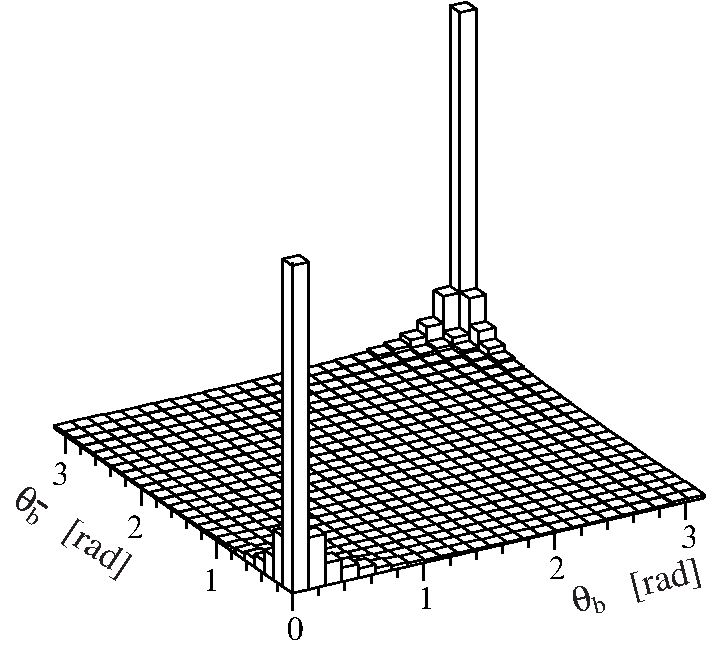
\includegraphics[ width=0.45\textwidth]{./Figs/LHC_LHCb/b_distrib_lhcb.pdf}
  \caption{Simulated angular distribution for \bbbar production at the LHC, angles are relative the the beam pipe with $\theta =0$ in the forward direction and $\theta = \pi$  in the backward direction~\cite{Amato:1998xt}.}
 \label{fig:bbar_production}
\end{figure}



The LHCb experiment was built as a single arm forward spectrometer, with an angular coverage of 10 to 300~mrad in the vertical direction and 10 to 250~mrad in the horizontal direction relative the the beam pipe. The angular coverage was chosen to exploit the small angles at which \bbbar pairs are produced. A cross-section of the LHCb detector is shown in Figure \ref{fig:LHCb_detector}, where a right handed coordinate system is used. Protons collide at the interaction point on the left hand side of the diagram, the products of the collisions travel through the detector leaving information in the sub-detectors along the length of the detector. The information deposited in the sub-detectors is reconstructed to determine what happened during the $pp$ collisions. 

\begin{figure}[htb] 
  \centering    
  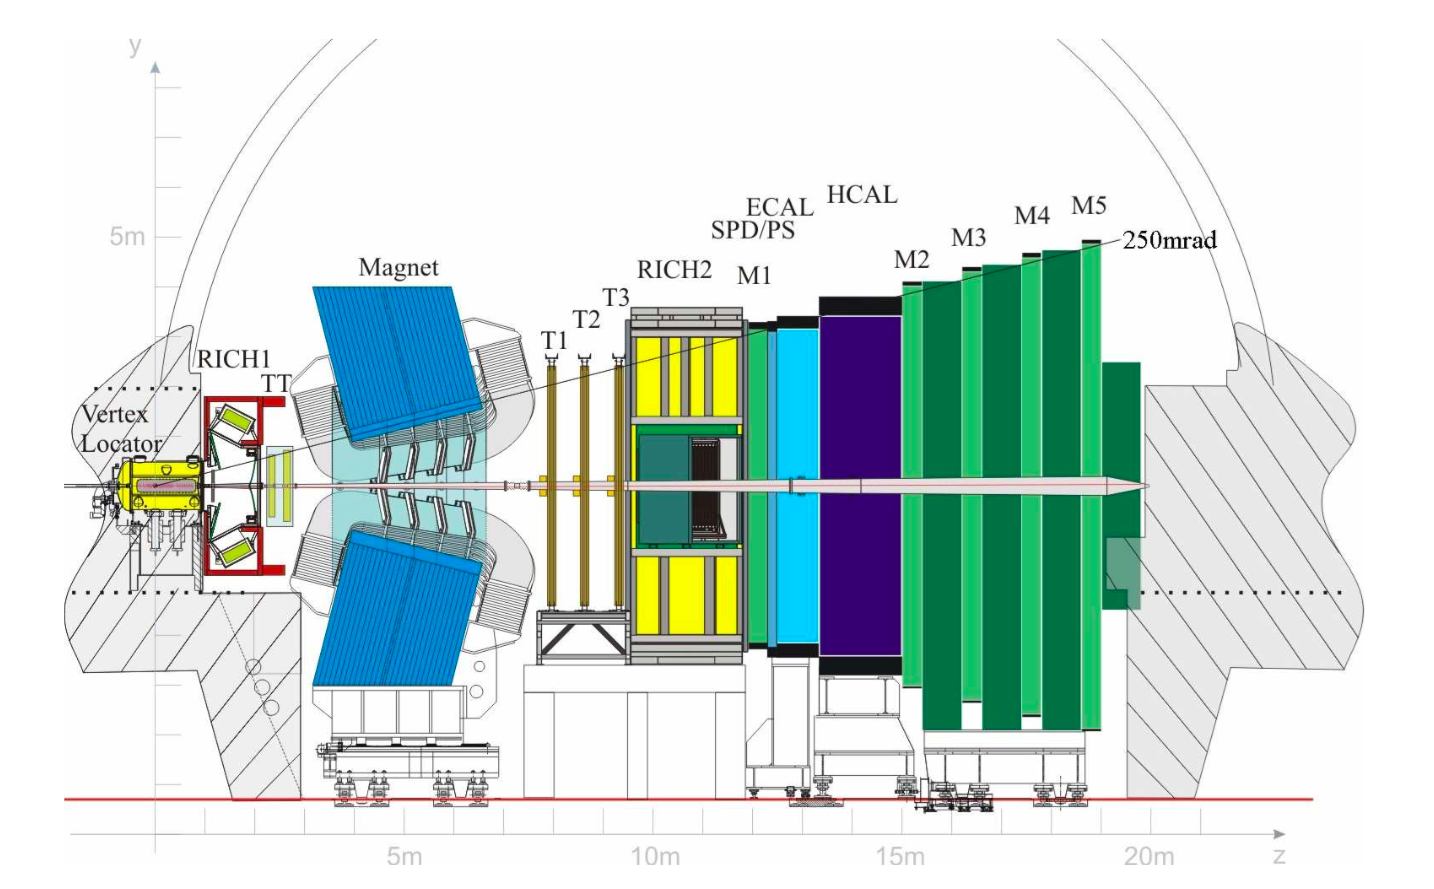
\includegraphics[ width=1.0\textwidth]{./Figs/LHC_LHCb/lhcb.png}
  \caption{Cross section of the LHCb detector \cite{Alves:2008zz}.}
  \label{fig:LHCb_detector}
\end{figure}


The different sub-detectors have been chosen to exploit the characteristics of \bhadron decays and fall into 2 distinct categories; tracking detectors and particle identification detectors. Each sub-detector and its performance are described in the following sections along with the trigger system and software needed to analyse the data collected by the experiment. %Finally the data recorded by the experiment during Run 1 and Run 2 is presented in Section \ref{LHCb_data}. 
For a more detailed description of the detector and its performance during Run 1 see \cite{LHCb:2003ab,Aaij:2014jba}.




\subsection{Tracking}
\label{Tracking}

The tracking system within the LHCb experiment consists of the vertex locator (VELO), a dipole magnet and the tracking stations. Together the sub-detectors provide precise information on the passage of charged particles through the detector and the particle momentum. 
The tracking detectors work on the principle that the passage of high energy charged particles through silicon or ionised gas causes the excitation or ionisation atoms in the material. The release of this energy is recorded and translated into an electrical signal that reveals the path of a particle. 
%Precise particle track and momentum measurements are necessary to obtain the accurate particle mass and decay time measurements that help distinguish between different hadrons decaying in the LHCb detector. 

\subsubsection{The Vertex Locator}
\label{VELO}
The vertex locator (VELO) is a silicon detector surrounding the interaction point. Its main goal is to provide precise information $pp$ interaction vertices and secondary decay vertices of particles produced. Information the VELO provides enables precise measurements of particle lifetimes and impact parameters of particles tracks necessary for physics analyses.


The VELO is made of two identical halves, each half consists of 21 stations containing two silicon sensors arranged along the beam pipe. The two halves of the VELO slot together and there is a small gap in the centre for the beams to pass through. The arrangement of sensors along the $z$ axis, shown in Figure \ref{fig:velo}, it designed so that the sensors cover the full LHCb acceptance and a charged particle within the detector acceptance will pass through at least three stations. In each station the two sensors measure different coordinates, one measures the $r$ coordinates of charged particles and the other measures the $\phi$ coordinates as shown in Figure~\ref{fig:velo_sensor}. The $r$, $\phi$ coordinates and the $z$ placement of the sensors are used to reconstruct charged particle trajectories. Cylindrical coordinates were chosen to allow fast reconstruction of particle trajectories in the VELO.

\begin{figure}[htb] 
  \centering    
  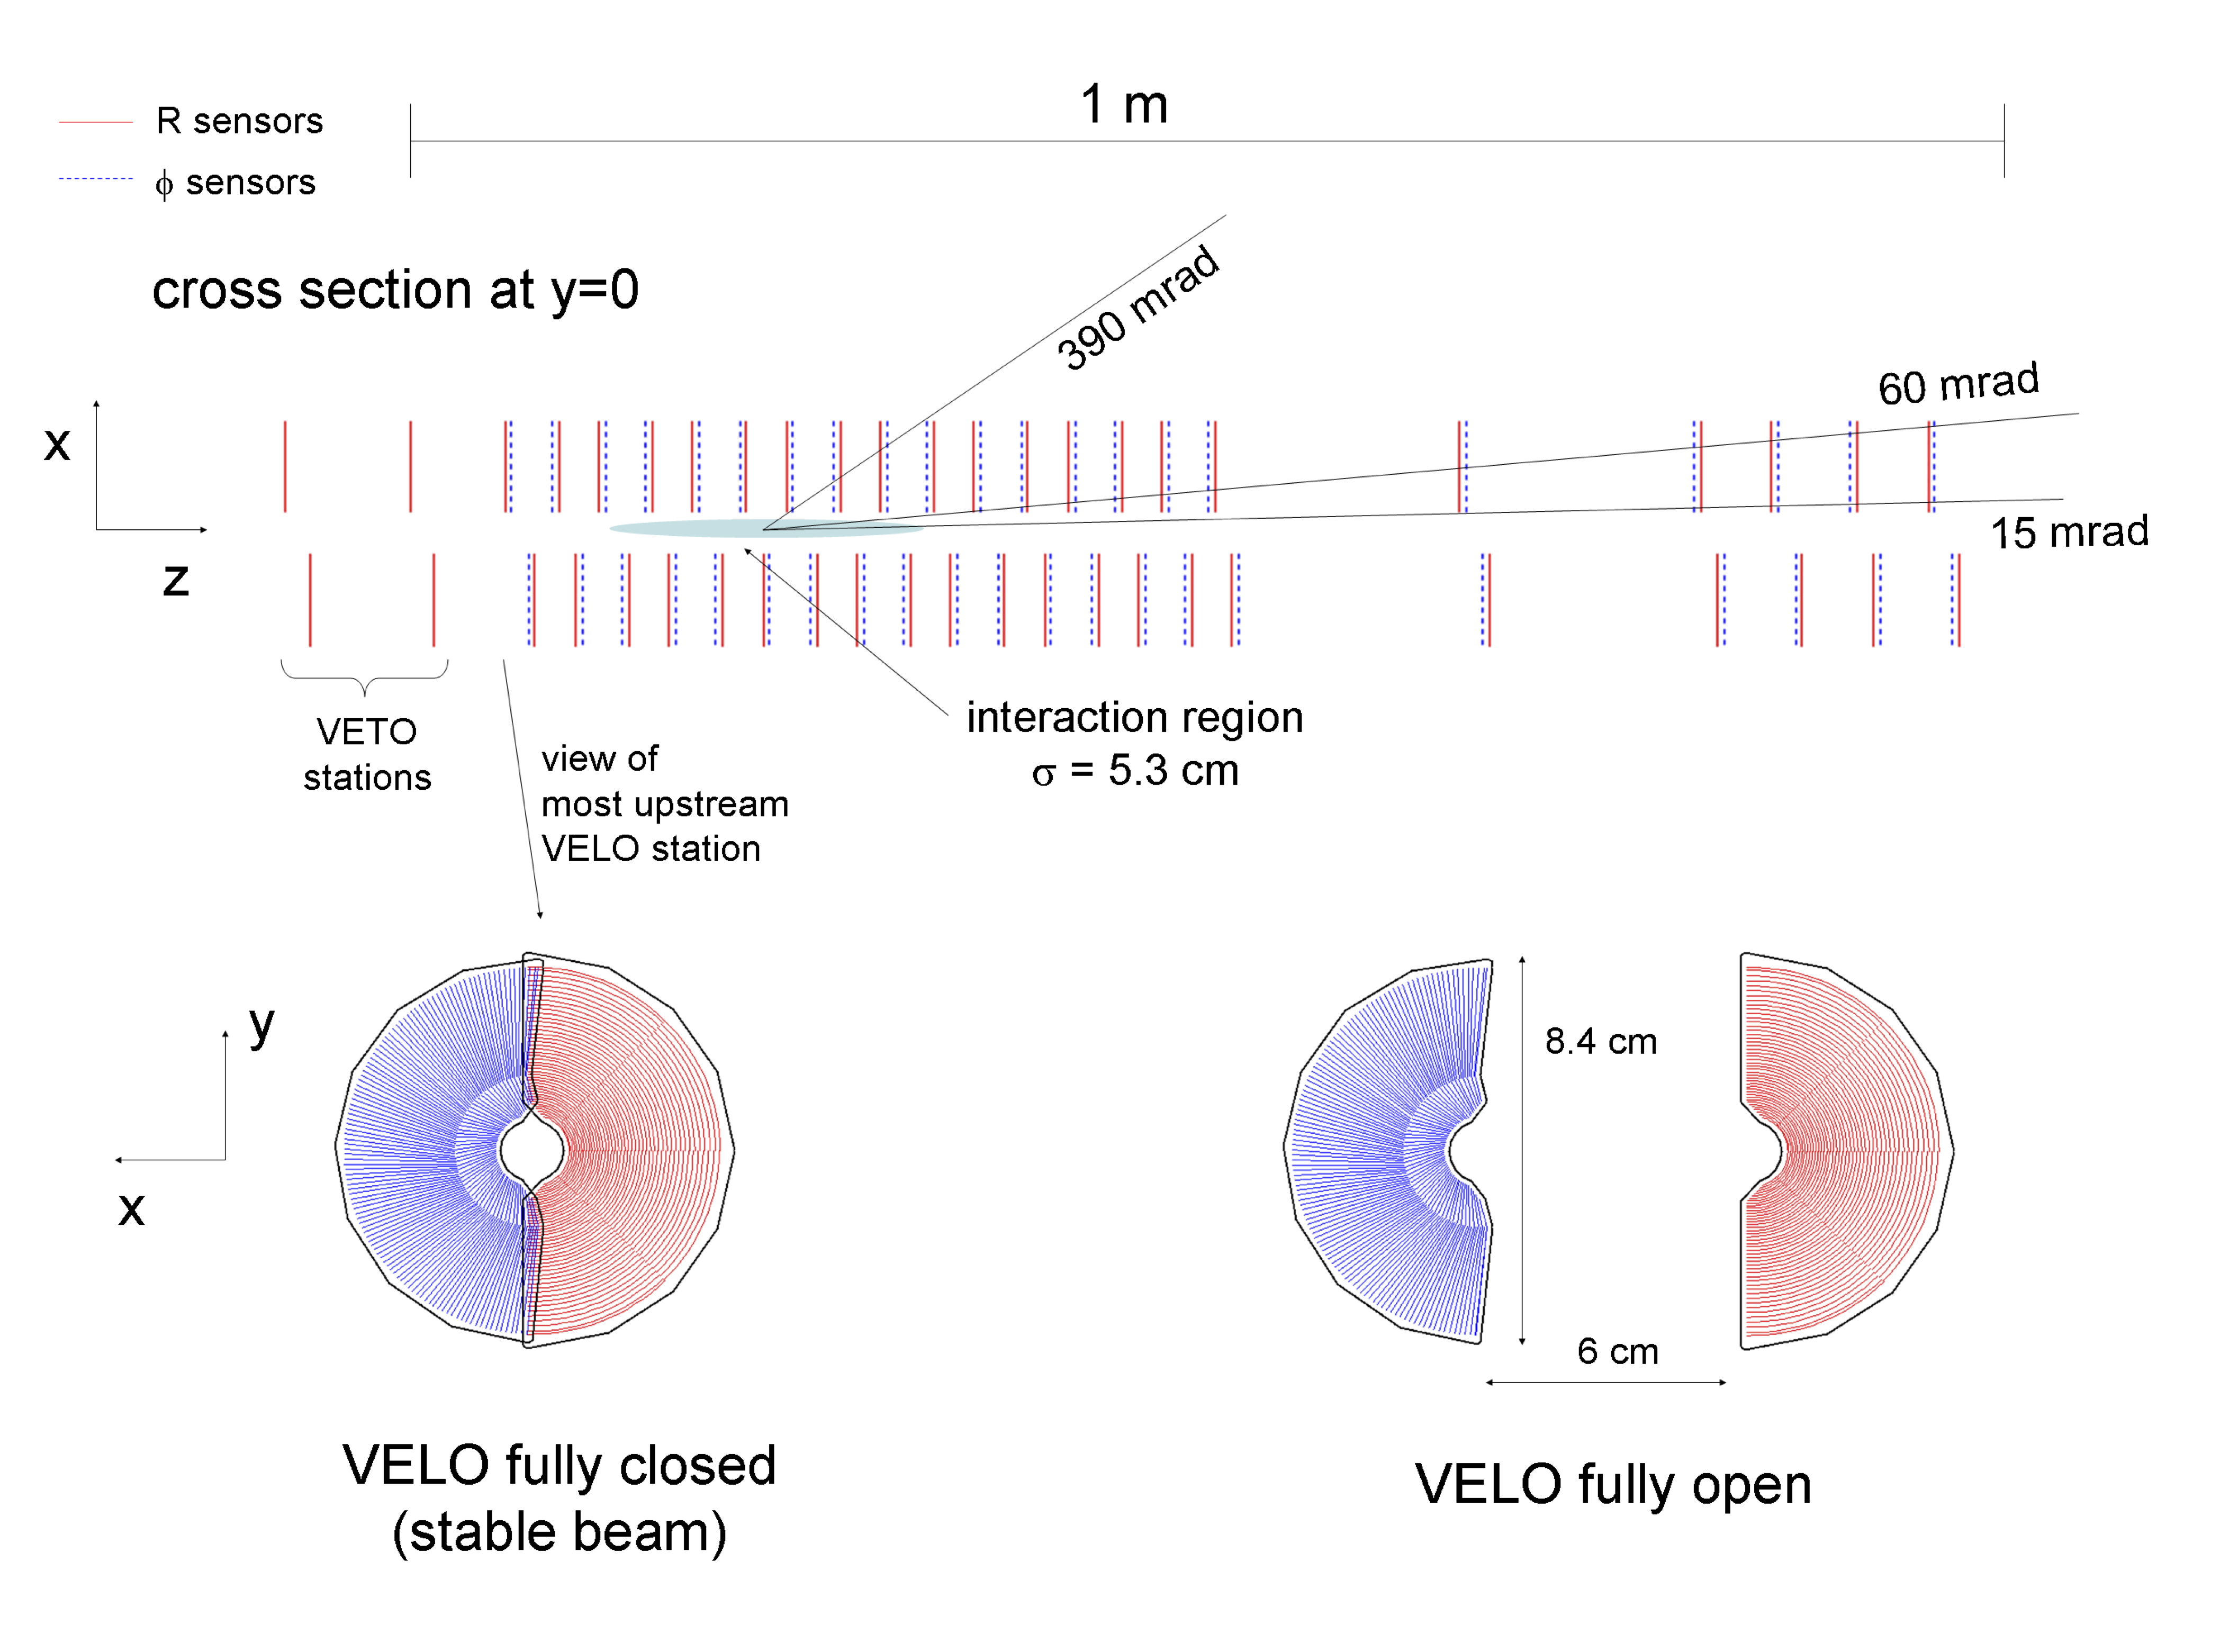
\includegraphics[ width=0.7\textwidth]{./Figs/LHC_LHCb/velo.png}
  \caption{The VELO layout and position of sensors along the beam axis \cite{Alves:2008zz}.}
  \label{fig:velo}
\end{figure}


\begin{figure}[htb]
  \centering
  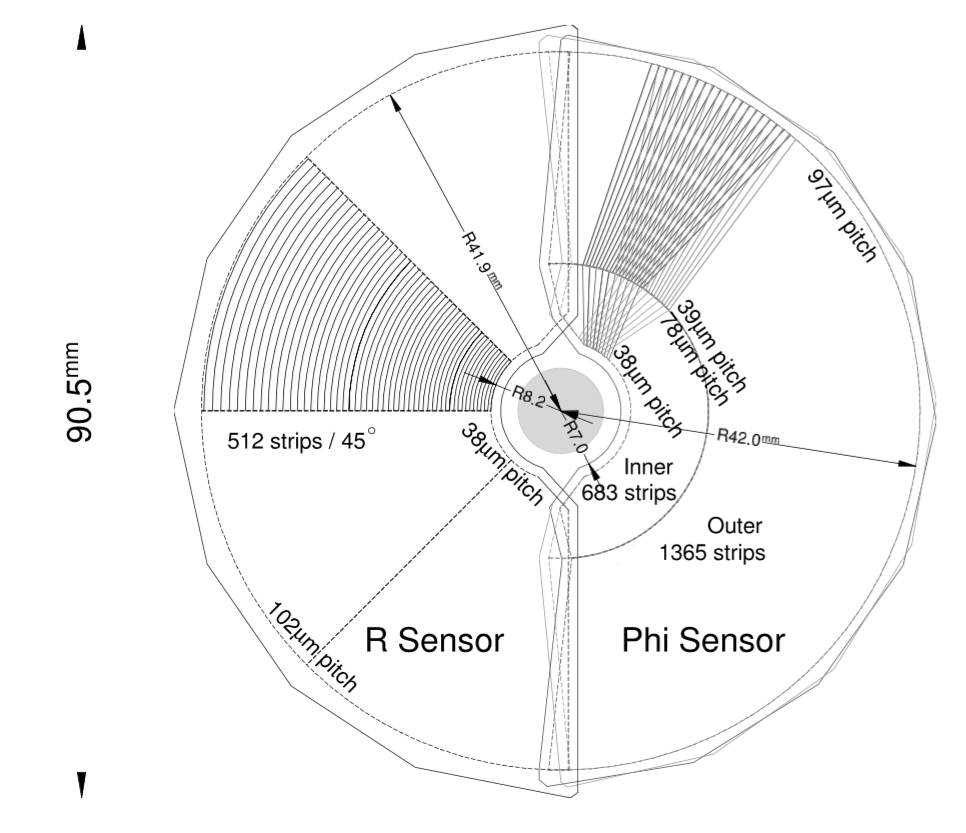
\includegraphics[ width=0.6\textwidth]{./Figs/LHC_LHCb/Velo_sensor_diagram.png}
  \caption{Diagram of $r$ and $\phi$ sensor layouts~\cite{Alves:2008zz}.}
  \label{fig:velo_sensor}
\end{figure}


The momentum resolution achievable for charged tracks by the LHCb experiment is limited by multiple scattering of particles as they travel through material in the detector. Therefore, to ensure good momentum resolution throughout the detector, the VELO is kept in a vacuum to reduce its material budget. Each half of the VELO is enclosed inside an aluminium box, which keeps it in a vacuum and shields the electronic readouts of the from radio frequencies generated by the beam. The overall material budget of the VELO comes to 17.5 $\%$ of a radiation length.

Excellent vertex resolution is required in the VELO, to acheive this the sensor need to be as close as possible to the interaction point. This is acheived by making the VELO out of two retractable halves and including the $pp$ interaction point within the coverage of the VELO. 
%The sensors of the VELO are located as close as possible to the $pp$ interaction point in order to acheive excellent vertex resolution. The VELO is made out of retractable halves and including the interaction point within the coverage of the VELO. 
During data taking, when the VELO is recording particle tracks the sensors are 8mm from the beam axis. However during the injection phase of the beam the width of the beam is much larger, therefore the halves of the VELO can retract to be 3~cm from the nominal beam axis. This keeps the VELO safe from unnecessary radiation damage. The two halves of the VELO are displaced by 150~mm in the $z$ direction, as shown in Figure~\ref{fig:velo} so that when the VELO is closed, the sensors in each half overlap to help with detector alignment and reduced edge effects. 

%\begin{figure}[htb] 
%  \centering    
%  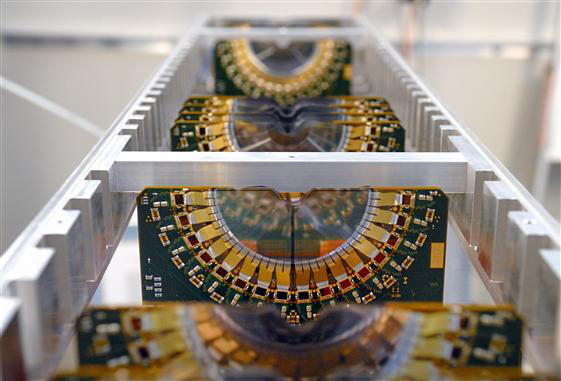
\includegraphics[ width=0.7\textwidth]{./Figs/LHC_LHCb/Velo_photo.jpg}% ./Figs/Detector/Velo_photo.jpg}
%  \caption{The velo Soure: LHCb.}
%  \label{fig:velo_photo}
%\end{figure}


%An additional purpose of the VELO is to act as a veto for high pile up events. There are 2 VELO sensors upstream of the interaction point that provide information to the trigger about how many $pp$ interactions there were with each bunch crossing. Events with large numbers of primary vertices are difficult and time consuming to reconstruct and lead to less precise measurements of particle decay properties. Information from the VELO is used to reject events with high numbers of primary vertices to ensure the best used of information from the detector.
An additional purpose of the VELO is to identify high pile up events. There are 2 VELO sensors upstream of the interaction point that provide information to the trigger about how many $pp$ interactions there were with each bunch crossing and this information can be used to identify events with high numbers of primary vertices. %Events with large numbers of primary vertices are difficult and time consuming to reconstruct and lead to less precise measurements of particle decay properties. 
%Information from the VELO can used to reject events with high numbers of primary vertices to ensure the best used of information from the detector.

The VELO achieves a vertex resolution of 10 - 20~$\mu$m transverse to the $z$ direction and 50 - 100 ~$\mu$m along the $z$ direction, the resolution of each track depends on the number of tracks in each event as shown in Figure~\ref{fig:Velo_PV_resolution}. The VELO also gives measurements on the impact parameters of particles tracks, which is the distance of closest approach between a particle track and the primary vertex. Figure \ref{fig:IP_res} shows the IP resolution for 2012 data, for a track with transverse momentum of 1~GeV/c is has an impact parameter resolution of 35~$\mu$m. 



%Can I just put the track resolution possible with the VELO?
\begin{figure}[tb] 
  \centering    
  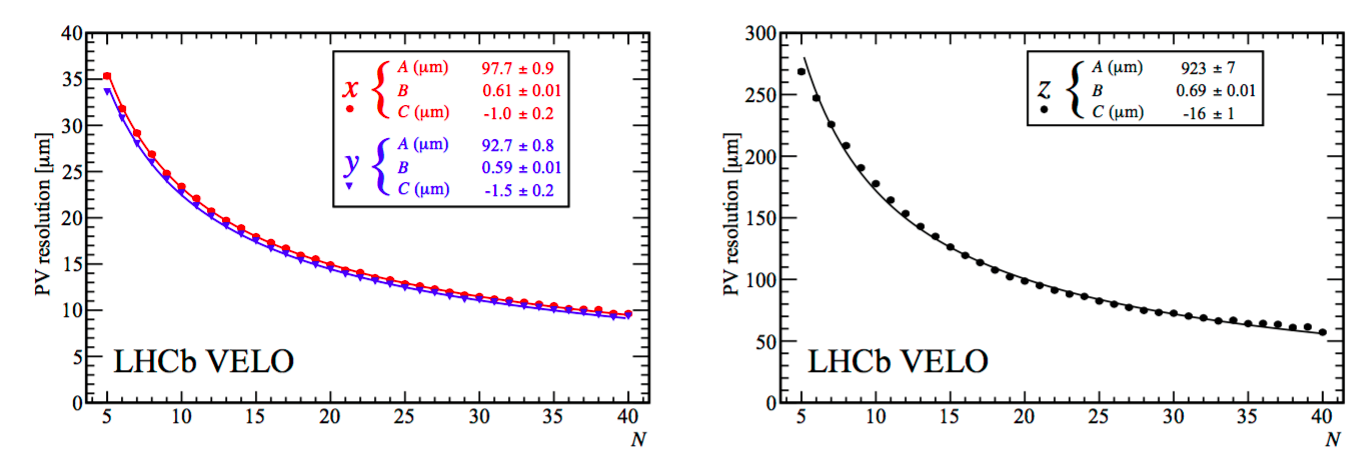
\includegraphics[ width=1.0 \textwidth]{./Figs/LHC_LHCb/Velo_vertex_resolution.png}
  \caption{Velo performance for primary vertex resolution perpendicular (left) and parallel (right) to the beam axis as a function of the number of tracks in an event for 2012 data~\cite{LHCbVELOGroup:2014uea}.}
  \label{fig:Velo_PV_resolution}
\end{figure}


\begin{figure}[tb] 
  \centering    
  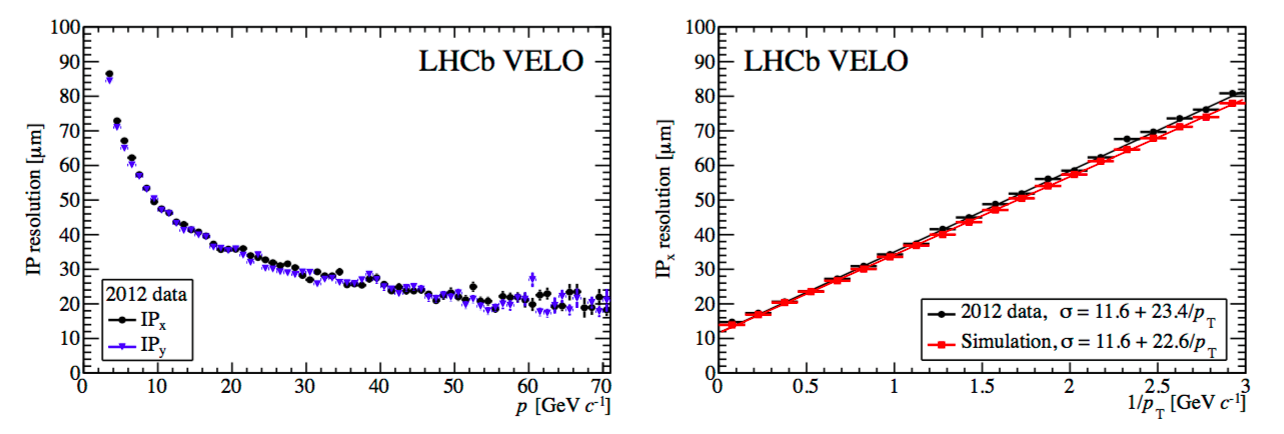
\includegraphics[ width=1.0\textwidth]{./Figs/LHC_LHCb/Velo_IP_resolution.png}
  \caption{Velo performance for impact parameter resolution as a function of momentum (left) and inverse transverse momentum (right) for 2012 data~\cite{LHCbVELOGroup:2014uea}.}
  \label{fig:IP_res}
\end{figure}


%Overall the VELO gives such and such precision.  vertex resolution in the transverse plane 10-20 mircons, in the z directions 50-100 microns depending on the number of tracks in the vertex. %The VELO is also important the impact parameter resolution and decay time resolutions.  (This may go at the end so that everything for tracking is together?) best resolution is 4 micrometers which allows a lifetime measurement of 50 fs. (Performance paper)



\subsubsection{Tracking Stations} 
\label{Tracking_Stations}
The LHCb experiment has 4 tracking stations in addition to the VELO, the Tracker Turicensis (TT) which is located upstream of the magnet and the T stations, T1-T3, located down stream of the magnet. These tracking stations provide complementary information to the VELO and the presence of the magnetic field allows the momentum of charged particles to be determined. 



The TT is made up of 4 layers of silicon trackers spaced 27 cm apart that cover the full LHCb angular acceptance. The TT is located just within the influence of the magnetic field of the dipole magnet, which provides the detector with 2 main purposes. Firstly, the TT tracks the passage of charged particles with high momentum to enable good momentum resolution of tracks when the information is combined with that from other tracking stations. The TT has a resolution of 50~$\mu$m for a single hit, this resolution was chosen so that multiple scattering in the detector material rather than detector resolution is the limiting factor for the momentum resolution. The second purpose of the TT is to record tracks of low momentum particles that are then swept out of the detector acceptance as they continue through the magnetic field. These tracks will have a lower momentum resolution but help with pattern recognition within the RICH detectors. 
%Information from just the TT and the VELO can provide an momentum accuracy of ~ 20 $\%$. 
%active area of 8.4m^2


The T stations, T1-3, are split into two sections, each composed of an Inner Tracker (IT) made of silicon and an Outer Tracker (OT) composed of straw drift tubes. 
There is a large increase in size of the tracking stations between the TT and the T3 so that all the detectors cover the full angular acceptance of the detector. The TT is 150~cm by 130~cm where as the T3 station is 600~cm by 490~cm, this is illustrated in Figure \ref{fig:size_of_tracking_stations}. The large size of the T stations meant that the high cost of silicon prevented it being used for the full coverage of each station.

\begin{figure}[htb] 
  \centering    
  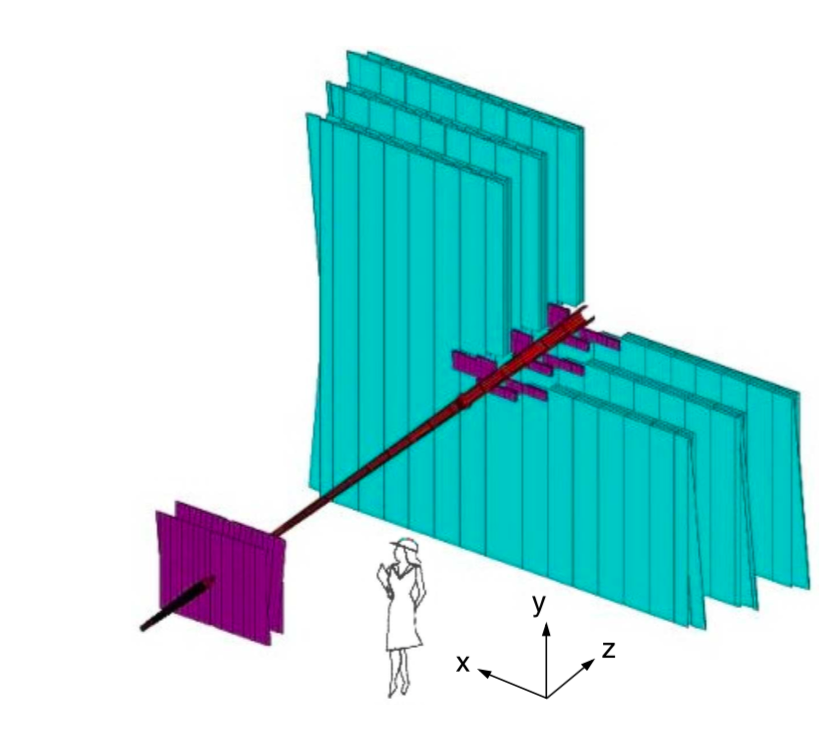
\includegraphics[ width=0.5\textwidth]{./Figs/LHC_LHCb/TT_IT_OT_comparison.png}
  \caption{Sizes of the TT and T stations~\cite{Alves:2008zz}.}
  \label{fig:size_of_tracking_stations}
\end{figure}

The IT has very similar in design to the TT, each station is made of 4 layers of silicon trackers with an overall track resolution of 50 $\mu$m.
%and has an active area of 4.0m2. 
The silicon trackers are arranged in a cross shape around the beam pipe, as shown in Figure \ref{fig:size_of_tracking_stations}, although the IT covers less than 2$\%$ of the T stations, 20$\%$ of tracks pass through it. This allows the occupancy of the OT to be less than 10$\%$ enabling a good overall track resolution from the OT despite it not being made of silicon. The OT of each tracking station is made of 2 staggered layers of straw tubes, they cover the remaining area required for cover the full LHCb angular acceptance which includes tracks bent by the magnetic field. The straw tubes have a fast drift time of 50~ns giving a better than 200~$\mu$m track resolution. 


\subsubsection{Dipole magnet}
\label{Magnet}
A warm dipole magnet is used to measure the momentum of charged particles travelling through the LHCb detector. In a magnetic field the trajectories of charged particles are bent and the particle momentum can be measured from the curve of the track. %from the radius of curvature of the particle track the particle momentum can be determined.

The magnet is located between the TT and the T stations and its field covers the full LHCb acceptance. The field is in the vertical direction therefore bending tracks in the horizontal direction. The magnet was designed so that the field strength in the RICH detectors is negligible (less than 2 mT) and to have the largest strength possible between the TT and T stations. Figure \ref{fig:Magnet_field} shows a plot of the magnet strength alongside the detector layout. A small magnetic field is achieved in the RICH detectors by iron shielding. The magnet was designed to have an integrated field strength is 4~Tm for track that travels 10~m through the detector.% and the peak strength is 1.1T. % I should maybe mention the measurement of the field and how it had to be accurate (with Hall probes) in order to get good momentum resolution but I don’t want to. The magnetic field strength enables the tracking systems to achieve a momentum resolution of $\delta p / p \~0.4\%$. 

\begin{figure}[htb]
  \centering
  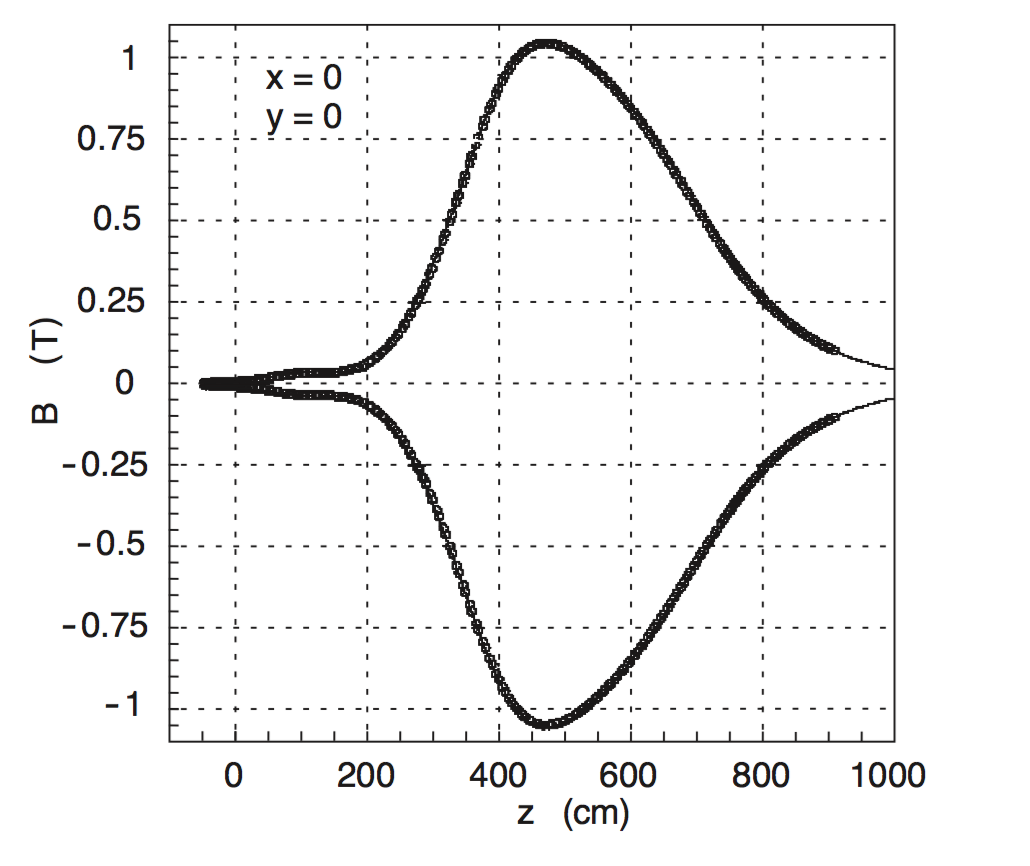
\includegraphics[ width=0.4\textwidth]{./Figs/LHC_LHCb/Magnet_field.png}
  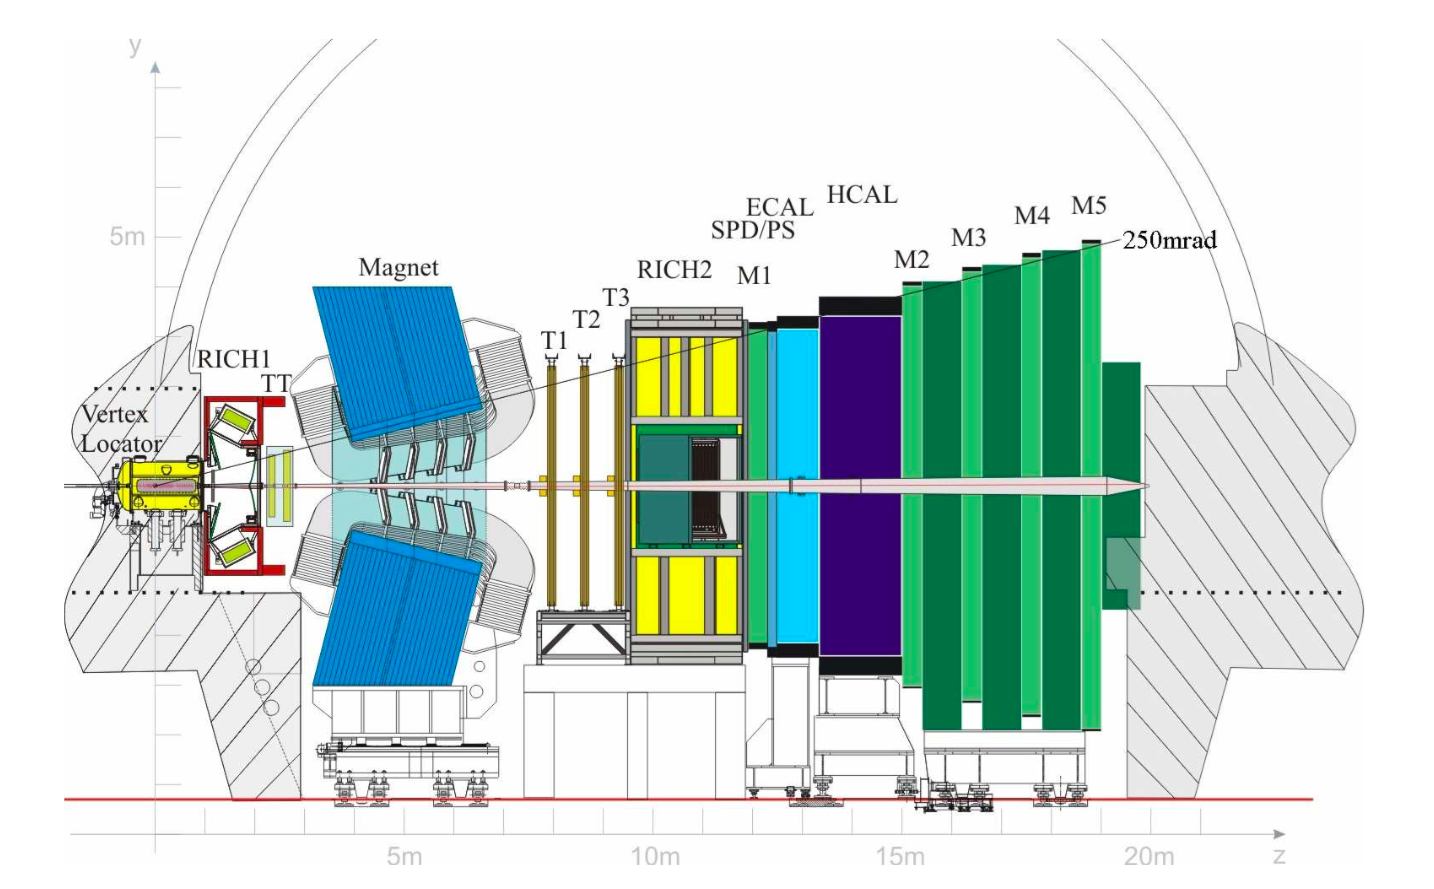
\includegraphics[ width=0.48\textwidth]{./Figs/LHC_LHCb/lhcb.png}
  \caption{Magnet field of the dipole magnet along the length of the LHCb detector (left) and the layout to the LHCb detector \cite{Alves:2008zz}. The peak strength of the field occurs between the TT and T1-3 station. }
  \label{fig:Magnet_field}
\end{figure}

%\begin{figure}[tb] 
%  \centering    
%  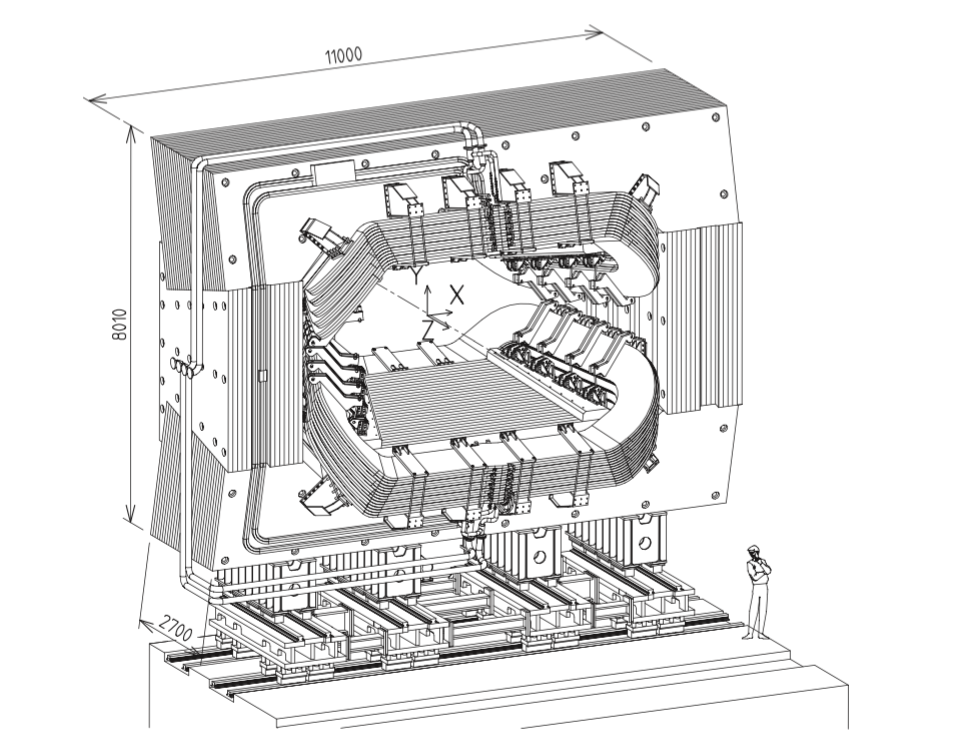
\includegraphics[ width=1.0\textwidth]{./Figs/LHC_LHCb/Magnet_picture.png}
%  \caption{Magnet picture. Source: \cite{Alves:2008zz}.}
%  \label{fig:types_of_tracks}
%\end{figure}


The polarity of the magnetic field is periodically switched so that is bends charged tracks in opposite directions. This is done so measure left-right detection asymmetries and to help understand systematic uncertainties of CP violation measurements. % These are not relevant for B2mm.



\subsubsection{Track reconstruction and performance}
\label{Track_recon}


The information left by the passage of charged particles through the VELO, TT and T stations is combined using track reconstruction algorithms to find trajectories of charged particles though the length of the LHCb detector and the particle momentum.  
The algorithms start with either segments of tracks in the VELO or the T stations and extrapolate from these segments into the other tracking detectors in specific search windows. 
Once the segments of the track have been found the trajectory is fitted with a Kalman Filter with takes into account multiple scattering and energy loss within the detector. For each track the filter returns the $\chi^{2}$ per degree of freedom, this is a measure of quality for the track. In LHCb this parameter is used to ensure that only good quality tracks are used in physics analyses. 
The reconstructed tracks are classified into five types depending on which detectors they travelled through, as shown in Figure \ref{fig:types_of_tracks}.



The different track classifications are:
\begin{itemize}
\item {\bf VELO tracks} are formed by particles produced at large angles to the beam axis or travelling in the negative $z$ direction from the interaction point, these particles only leave tracks in the VELO. VELO tracks are useful for reconstructing primary vertices.  
\item {\bf Upstream tracks} are made by low momentum particles that only leave hits in VELO and TT which are upstream of the magnet. The absence of tracks further down the detector is because the magnetic field sweeps the particles out of the detector acceptance. Upstream tracks have poor momentum resolution but are useful for understanding backgrounds and pattern recognition in the RICH~1 located between the VELO and the TT.
\item {\bf Downstream tracks} are produced by the decays of long lived neutral particles, that travel out of the VELO before decaying. These particles only leave tracks the TT and T stations. 
\item {\bf T tracks} are tracks that only cross the T1-3 stations and are formed from particles created in interactions with the detector material. Similarly to upstream tracks, T tracks can help to understand backgrounds and pattern recognition in the RICH~2 located just before the T stations.
\item {\bf Long tracks} are the most useful for physics analyses because they are formed by particles that travel through the VELO, TT and T1-3 stations. Information from all the tracking stations is combined so these tracks have the best momentum resolution.
\end{itemize}


\begin{figure}[tb] 
  \centering    
  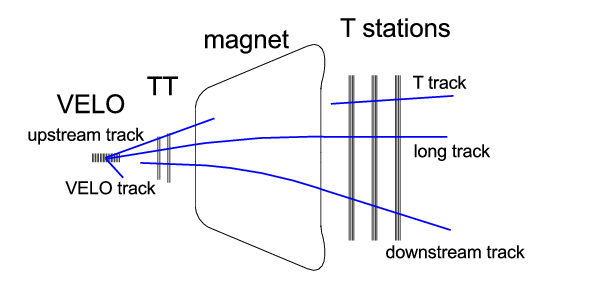
\includegraphics[ width=0.8\textwidth]{./Figs/LHC_LHCb/Types_of_tracks.png}
  \caption{Different types of tracks that are reconstructed at LHCb~\cite{Aaij:2014pwa}.}
  \label{fig:types_of_tracks}
\end{figure}

The efficiency to correctly reconstruct tracks varies with the particle momentum and the number of tracks present in an event, as shown in Figure~\ref{fig:types_of_tracks} for 2012 data. In Run 1 long tracks were correctly reconstructed on average of 96~$\%$ of the time.





\begin{figure}[tb] 
  \centering    
  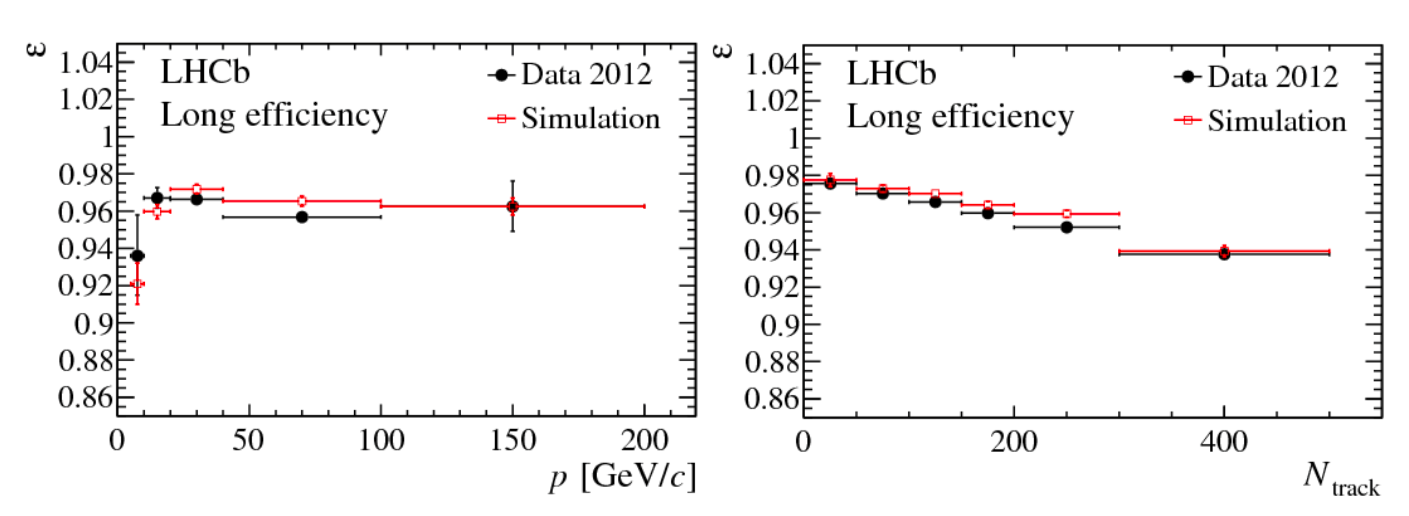
\includegraphics[width=1.0\textwidth]{./Figs/LHC_LHCb/LongTrack_efficiencies.png}
  \caption{Long track reconstruction efficiency as a function of momentum (left) and number of track in the event (right) for 2012 data \cite{Aaij:2014pwa}.}
  \label{fig:types_of_tracks}
\end{figure}




Inevitably not all tracks that are reconstructed are correct, there are two main types of incorrectly reconstructed tracks. The first are clone tracks that occur when two tracks have many hits in common, when this happens the track with the highest number of total hits it used and the other is discarded. The second type of incorrect tracks are ghost tracks that are formed when track segments in different detectors are incorrectly joined together. This most offen occurs with segments in the VELO and T1-3 stations, the number of ghost tracks in an event depends on the event multiplicity. These tracks are removed by cutting on the output of a neural network that returns a probability of how likely a track is to be fake.



Once the tracks have been reconstructed, parameters that are necessary for the identifying and measuring different particles decays in an event can be computed from the tracks. The combined tracking systems achieve a momentum resolution of $\delta p / p = 0.5\%$ for particles with $p$ =  20~GeV/c and a resolution of $\delta p / p = 0.8\%$ for particles with $p$ =  100~GeV/c.  This momentum resolution, when combined with vertex information from the VELO, gives a decay time resolution of around 50~ns. 



%The performance of the tracking system has been studied of Run 1 data \ref{ performance paperS}. The tracking system provide measurement of the momentum of the charged particles that it tracks, good momentum resolution is required in order to obtain good mass resolution which is necessary to identify different  b hadrons and to distinguish between signal and background events. The momentum resolution of long tracks is shown in figure  OR the momentum resolution is $\delta$p/p = X - Y $\%$ which depends on the momentum of the reconstructed track. 


%The tracking system allows accurate reconstruction of primary vertices, this is necessary to measure time dependant processes, lifetimes and identify decaying particles. It was particular important for LHCb so that is could measure the rapidly oscillation Bs system. The PV resolution has been measured on 2012 data and varies with the number of tracks used to reconstruct the vertex, on average the vertex resolution transverse to the beam is between 10 and 25 mum and parallel to the beam is  between 50 and 150 mum for the z direction as shown in figure \ref{fig:types_of_tracks} for 2011 data. %Ref veto paper.



%The impact parameter is another important variable, it measure the distance of closest approach of a track to the PV, long lived particles tend to have a large IP wrt to PV because they travel before they decay. Good measurements of the IP help to remove prompt backgrounds. The IP resolution depends on the momentum of the particles and Figure \ref{fig:types_of_tracks} shows the IP resolution for 2012 data, for a track with transverse momentum of 1 GeV/c is has an IP resolution of 35 mum.

%Finally, the measurement of lifetime of b hadrons at LHCb needs accurate decay time measurements but more importantly to understand the rapidly oscillating Bs system good decay time resolution is needed. To reconstruct the decay time information about particle momentum and decay length, how far the particle travelled before it decays are needed. Therefore good PV resolution and moment resolution are needed. The LHCb detector achieved typically 50 ns resolution on the decay time. 



\subsection{Particle identification}
\label{PID}

In LHCb the particle identification (PID) detectors consist of two ring imaging Cherenkov (RICH) detectors, electromagnetic and hadronic calorimeters and muons stations. Together these detectors distinguish between different charged leptons and hadrons and between neutral particles such as photons and neutral pions. Good particle identification is necessary to determine which \bhadron decayed and to distinguish between topologically similar decays, such as \bdkpi, \bskk and \bmumu. %This could be out elsewhere perhaps in the RICH specific part?



\subsubsection{Ring Imaging Cherenkov detectors}
\label{RICH}
%There is a plot that shows the usefulness in comparing 2 mass plots of the RICH PID, this is in Ed Greening's Thesis. It could be nice to include this, or something like it because it is very relevant to Bs2MuMu and the verification of the lifetime measurement methods that I did. 

RICH detectors are used at LHCb to distinguish charged hadrons and leptons that have a momentum between 2 and 100~GeV/c. The RICH detectors are vital to distinguish between pions, kaons and protons frequently produced in \bhadron decays. %This needs to be done because correctly reconstructing the b hadron invariant mass relies on correctly identifying what it decayed into. Information from the RICH is particularly important at distinguishing different b2hh decays which is useful for this thesis. 
The energy range of the RICH detectors was chosen because the typical decay products of 2-body \bhadron decays is around 50~GeV. 



The RICH detectors are based on the following principle; when a charged particle travels with velocity $v$ through a dielectric medium with a refractive index $n$, the atoms excited by its passage are polarised, if the particle is travelling faster than the speed of light in the medium the excitation energy is released as a coherent wavefront. The angle, $\theta_{c}$, the wavefront travels at relative to the particle trajectory depends on the speed at which the particle was travelling as $cos(\theta_{c}) = c/nv$. The light is produced in a ring and is called Cherenkov radiation. %The RICH detectors measure the angle of light produced as particles pass through them, the angle gives a measurement of the particle’s speed which when combined with momentum from the tracking stations gives that particle’s mass and therefore its identity. 
The angle at which Cherenkov radiation is produced gives a measurement of a particle’s speed which when combined with the particle’s momentum, the particle mass and consequently its identity can be determined. However many particles travel through the RICH detectors and create overlapping rings of light making particle identification complex. Particle trajectories through the RICH detectors are inferred from information in the tracking stations and the expected pattern of Cherenkov radiation is calculated for each possible particle type. The expected patterns of light are compared to the observed pattern to find the likelihood for each particle type, all possible particle types are compared to maximise the likelihood. An in depth description of the reconstruction algorithm used in the RICH detectors can be found in~\cite{Forty:684714}. 


\begin{figure}[htb]
  \centering
  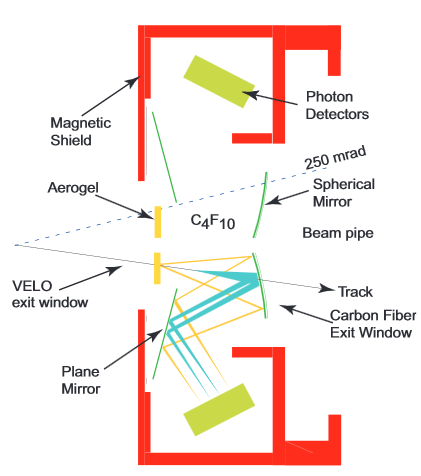
\includegraphics[ width=0.40\textwidth]{./Figs/LHC_LHCb/RICH1diagram.png}
  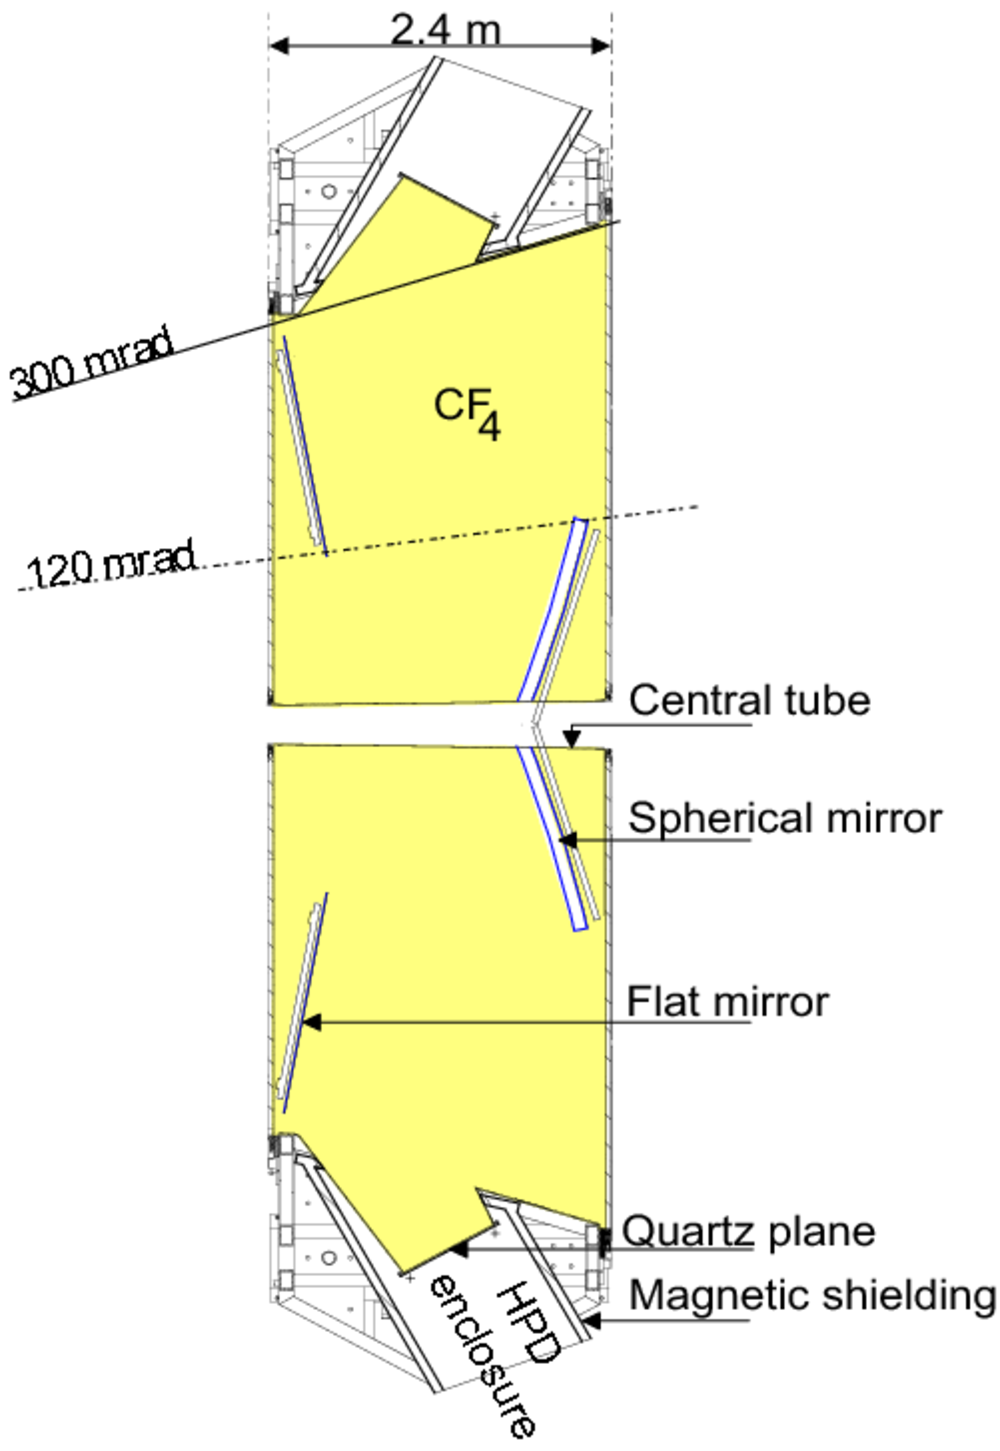
\includegraphics[ width=0.3\textwidth]{./Figs/LHC_LHCb/rich2_schematic.png}
  \caption{Diagram of the RICH1 detector (left) and the RICH 2 detector (right)~\cite{Alves:2008zz}. For Run 2 the aerogel radiator in the RICH~1 detector was removed.}%, also Olli has a nice picture of a HPD schematic.}
  \label{fig:RICH_diagram}
\end{figure}


The two RICH detectors cover complimentary momentum regions. The RICH~1 detector is located between the VELO and the TT station, it covers the full LHCb angular acceptance and provides PID information on particles in the momentum range 1 to 40~GeV/c. The RICH~1, is illustrated in Figure~\ref{fig:RICH_diagram}, it contains two different radiator materials; at the front of the detector is a aerogel sensitive to particles with a momentum between 2 and 10~GeV/c, behind the aerogel is a gas radiator sensitive to particles in the momentum range 10 to 40~GeV/c. The aerogel radiation was removed after Run 1, therefore the RICH~1 is only sensitive to particles in the momentum range 10 to 40~GeV/c in Run~2. As charged particles travel through the RICH~1, the rings of light produced are focused by spherical mirrors onto Hybrid Photon Detectors (HPDs), the radii of the detected rings provides information about how fast the particle was travelling. %The speed of the particles, when combined with information about it’s momentum from the tracking stations realise the particles mass and therefore it’s identity.



The RICH~2 detector is located upstream of the RICH~1, between the last tracking station and the first muon station. The RICH~2 consists of a gas radiator sensitive to particles with a momentum range 15~-~100~GeV/c and the detection of the light produced is the similar to the RICH~1 as illustrated in Figure~\ref{fig:RICH_diagram}. Unlike the RICH~1, the RICH~2 detector does not cover the full LHCb angular acceptance but only $\pm$~120~mrad in the horizontal and $\pm$ 100 mrad in the vertical direction. This area contains the higher momentum particles the RICH~2 is sensitive to, the low momentum particles have been bent out of the acceptance by the magnetic field. 


Both RICH detectors use HPDs that are sensitive to magnetic fields, the HPDs are shielded from the magnet field using iron sheets ensuring the field is less than 2mT across them. This allows accurate detection of light created within the RICH detectors.
 
The rings of light collected by the RICH detectors when combined with information about particle momentum and tracks from the tracking stations enables the particle type to be identified. Figure \ref{fig:RICH_preformance} shows how the Cherenkov angle and momentum can be combined to identify different types of particles in the RICH~1 detector, there are distinct bands for each particle mass. Figure \ref{fig:RICH_radiator_predictions} shows what is expected for the different radiators.  

\begin{figure}[htb]
  \centering
  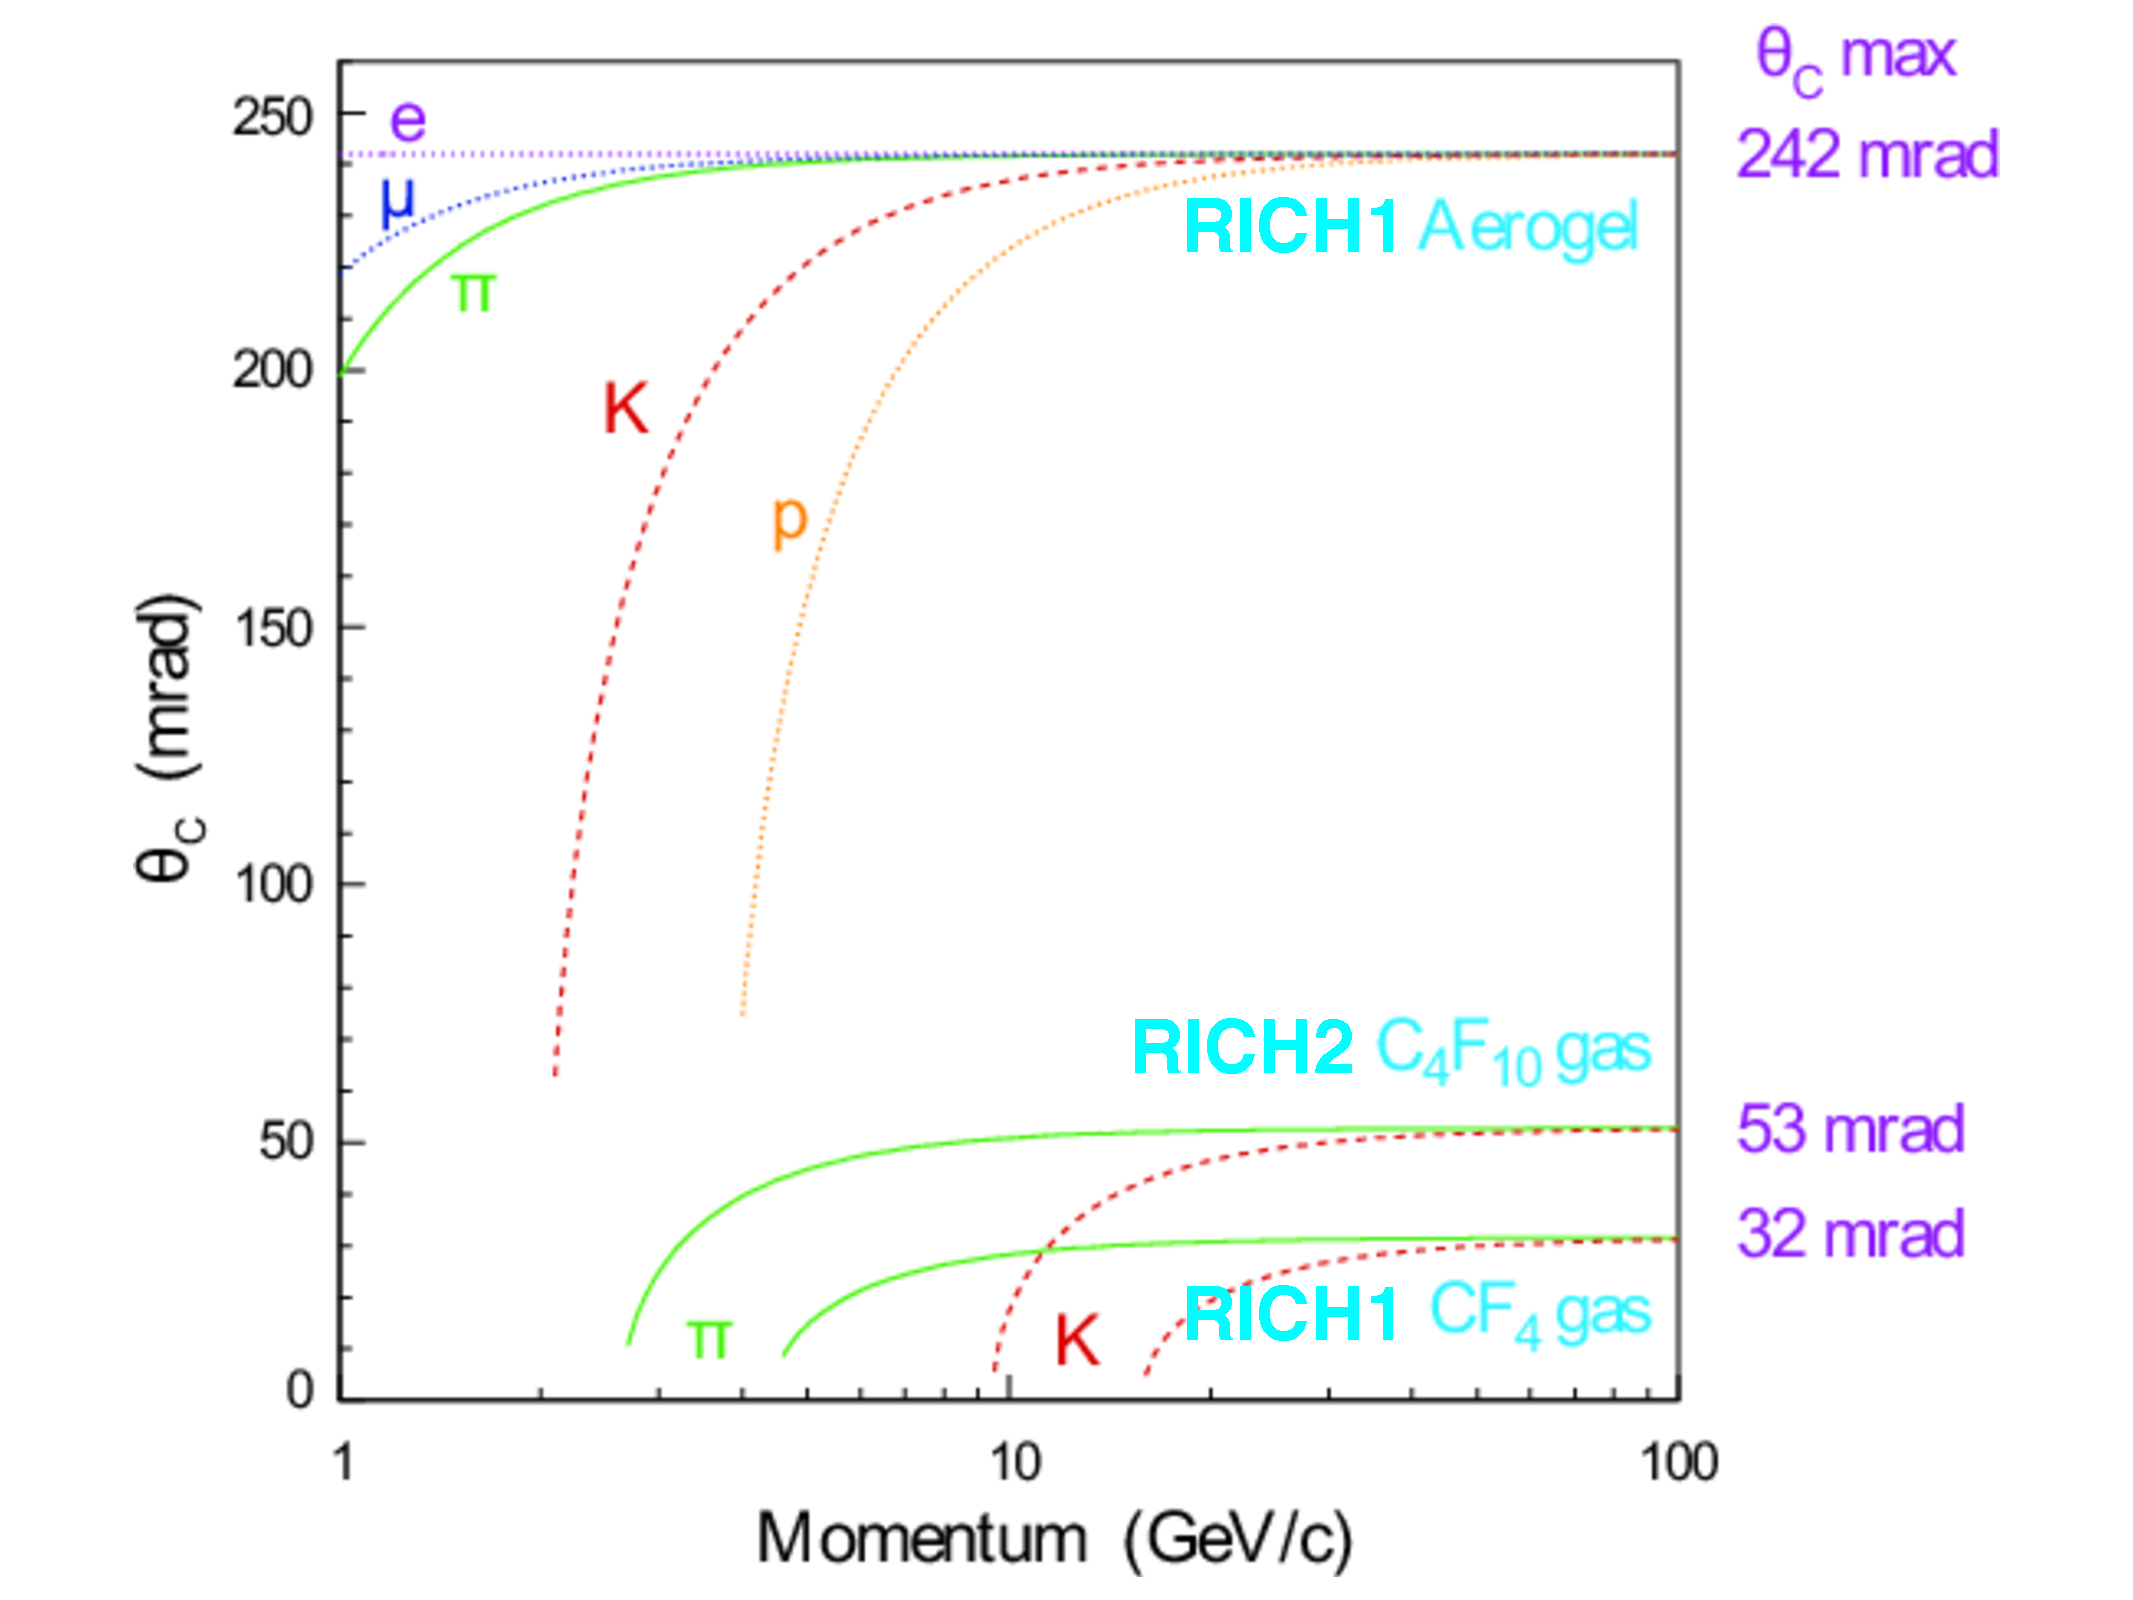
\includegraphics[ width=0.7\textwidth]{./Figs/LHC_LHCb/RICH_radiators.pdf}
  \caption{Expected Cherenkov angles produced by different particles travelling through the radiators in the RICH detectors~\cite{Alves:2008zz}.}
  \label{fig:RICH_radiator_predictions}
\end{figure}


\begin{figure}[htb]
  \centering
  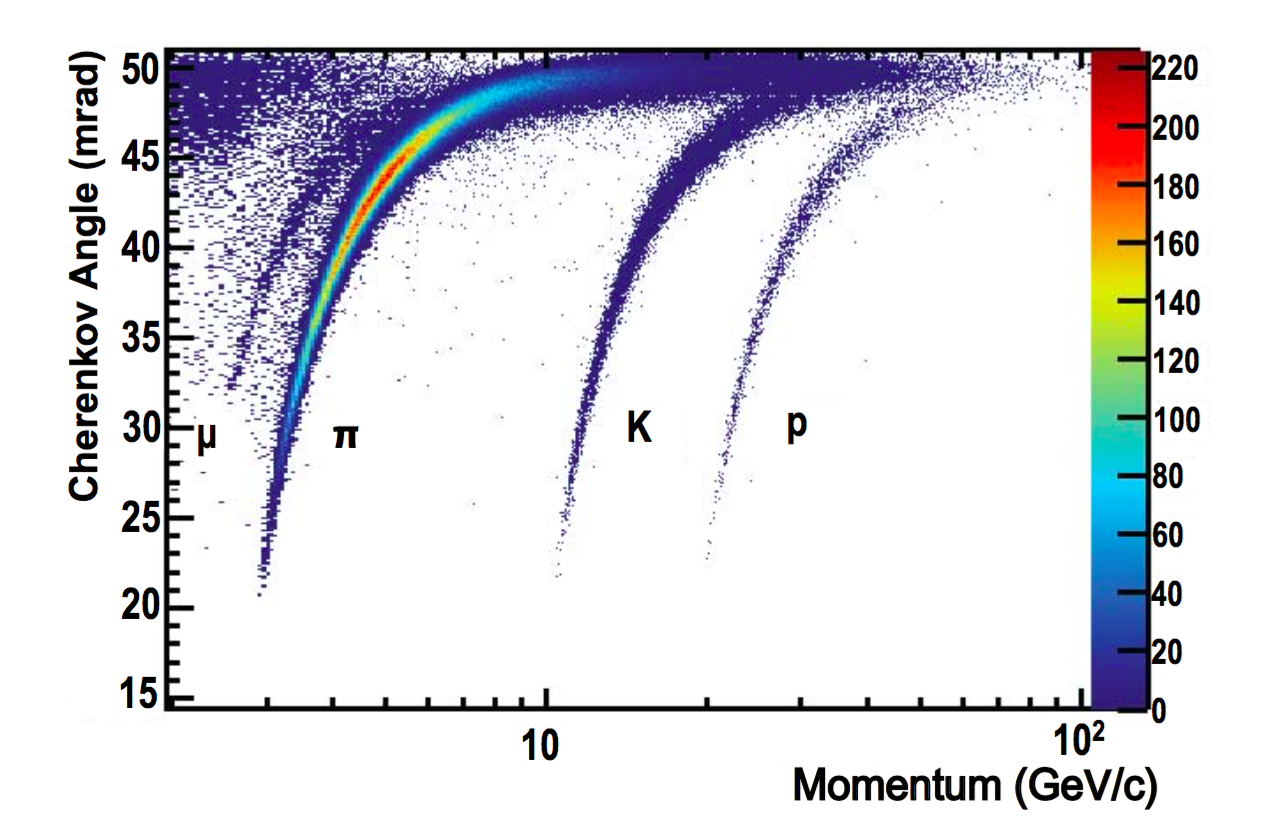
\includegraphics[width=0.8\textwidth]{./Figs/LHC_LHCb/RICH1_performance.png}
  \caption{Cherenkov angles for isolated tracks as a function of momentum in the RICH~1 detector for 2011 data \cite{Adinolfi:2012qfa}.}
  \label{fig:RICH_preformance}
\end{figure}


\subsubsection{Calorimeters}
\label{Calo}

The calorimeter system consists of the Scintillating Pad Detector (SDP), Pre-Shower (PS), electromagnetic calorimeter (ECAL) and the hadronic calorimeter (HCAL). Information from the calorimeters is used to identify electrons, photons and hadrons with high transverse momentum to be used in the first level of the trigger and to help with the reconstruction and identification of these particles. The ECAL is the only part of the LHCb detector that measures the position and energy of photons and neutral pions. 

The calorimeters in LHCb are sampling calorimeters that consist of layers of lead absorbers and scintillating material. In lead, incident particles create showers of secondary particles, the charged particles produced in the absorbers create light as they pass through the scintillators. The light travels through wavelength shifters where it is collected by photon multiplier tubes and turned into an electrical signal. In the ECAL showers are started by ionisation, bremsstrahlung radiation or pair production depending on the energy of the incident particle and whether is it a $e^{\pm}$ or a photon. In the HCAL it is interaction via the strong force that leads to showers of secondary particles. The showers produced in the calorimeters are along the direction of flight of the incident particle. Unlike other sub-detectors in LHCb, the calorimeters change the particle as it moves through the detector in order to measure the energy.

The SPD, PS and ECAL identify electrons, positrons and photons. The SPD is a layer of scintillating material at the start of the calorimeter system, it separates electron and photon showers created later in the calorimeter because only charged particles will produce light in the SPD. Next in the calorimeter system is the PS, it consists of a lead absorber followed by another scintillator similar to the SPD, the length of the lead absorber is chosen so that electrons will start showers in the absorber but charged pions will not. There is only a 1$\%$ chance of a pion creating shower in the PS. Information collected by the PS enables showers created by pions in the ECAL to be separated from those created by electrons and positrons. The ECAL is designed to contain the entire shower of high energy photons so that it can provide good energy resolutions of photons passing through the detector. The ECAL has an energy resolution of $\delta E / E = 9\%/\sqrt{(E)} \oplus 0.8\%$  provided information from the PS and SPD are used. 

The HCAL is predominately designed for use in the trigger and there is no requirement that the HCAL contains the full hadronic showers, therefore it was designed with a lower energy resolution of $\delta E / E = 69\% / \sqrt{(E)} \oplus 9\%$. 


\subsubsection{Muon stations}
\label{Muon_stations}

The muons stations are designed to identify highly penetrating muons, for use in the trigger and offline analyses. Muons are produced in many \bhadron decays, good muon identification is necessary trigger events containing muons and to distinguish topologically similar decays such as \bmumu and \bdkpi in physics analyses. 
Compared to other particles muons have a high penetrating power due to their relatively large mass and because muons do not interact via the strong force, these properties are exploited in the muon detectors. 

There are 5 muon stations, M1-5, shown in Figure \ref{fig:muon_system} that track and identify muons. The first muon station is located before the calorimeters, the inner section where the fluence is greatest, is made of gas electron multiplier foils and the outer section is made from multiwire proportional chambers (MWPCs). Stations M2-5 are located after the HCAL, by which point most other particles have been absorbed by the calorimeters. These stations are made from MWPCs and between each station is 80cm of lead absorber ensuring only high energy muons pass through the muon detector. A muon must have a momentum of at least 3 GeV/c to pass through the calorimeters and the M2 and M3 stations, to travel through all the muons stations a muon must have a momentum of 6~GeV/c. 
The first 3 stations have a high spatial resolution and provide track and transverse momentum information to be used the the trigger. M1 is located before the calorimeters to improve the transverse momentum measurement of the muons. The last two stations have a lower spatial resolution and are designed to identify muons with the greatest transverse momentum. After the muon stations there is an iron wall to stop any particles from travelling downstream of the detector. The size of the muon stations increases with distance from the interaction point to ensure the full angular acceptance of the detector is covered. Tracking information collected in the muon stations can be used in the trigger because the stations lie outside the magnetic field which allows for fast reconstruction of the tracks and a muons. 

\begin{figure}[tb]
  \centering
  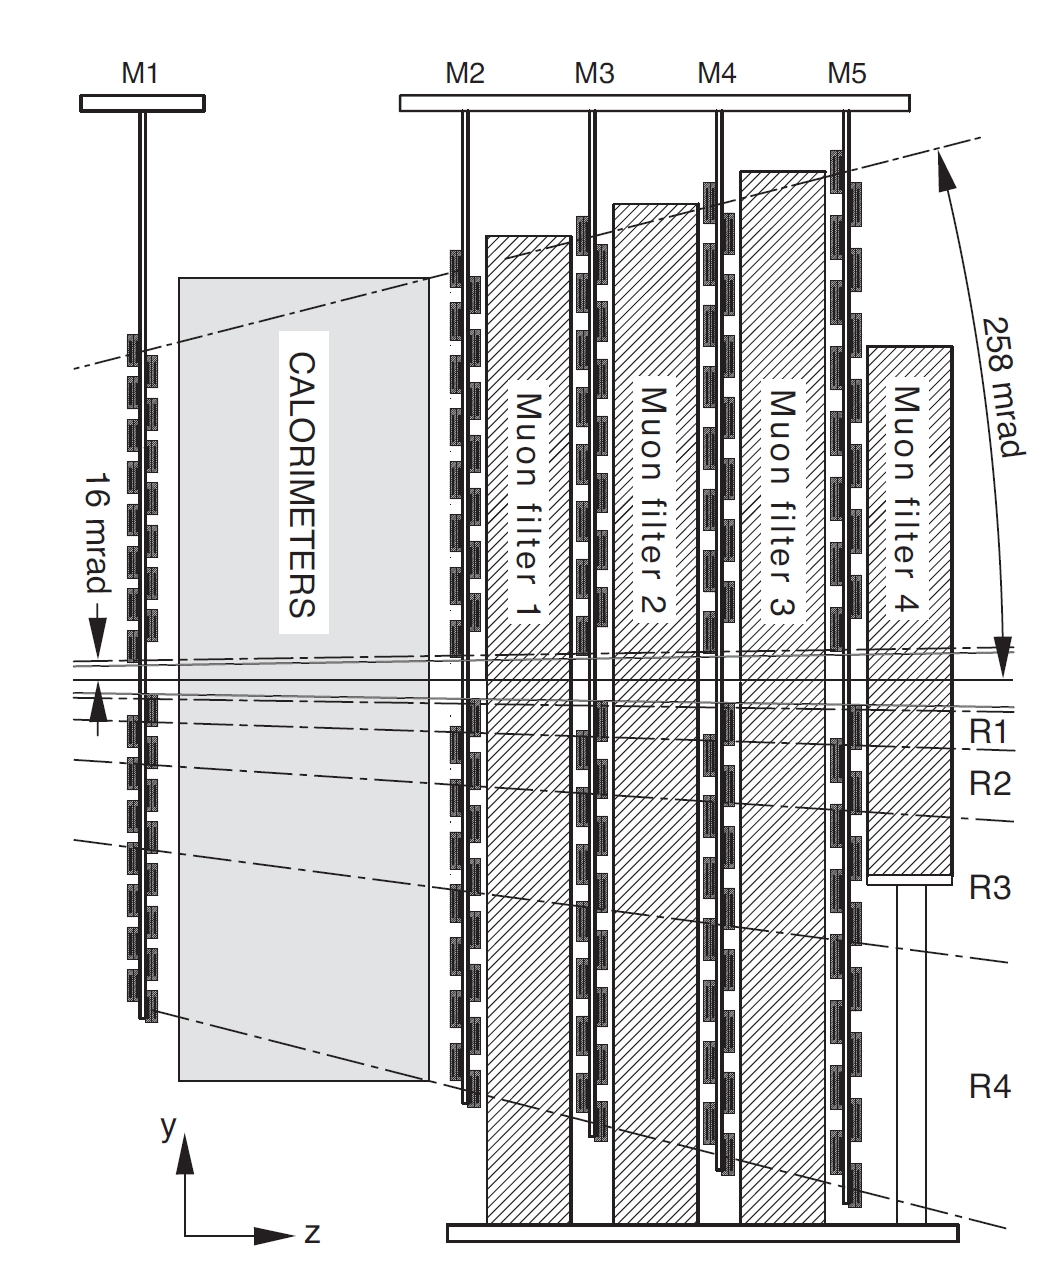
\includegraphics[ width=0.5\textwidth]{./Figs/LHC_LHCb/muon_system.png}
  \caption{Layout of the muon stations~\cite{Alves:2008zz}.}
  \label{fig:muon_system}
\end{figure}

\subsubsection{Particle identification and performance}
\label{PID_variables}
%There is a plot that shows the usefulness of the RICH PID, this is in Ed Greening's Thesis. 

The information collected in the PID detectors is combined to provide several discriminating variables that can be used to identify muons, protons, kaons, pions and electrons.

The muon stations are used, along with information from the tracking system, to produce a binary selection (isMuon) to identify muons. The tracking system is used to extrapolate a field of interest within the muon stations, a muon is identified if hits in the muon stations can be combined with those from the tracking system within the field of interest. The number of the hits required in the muon stations depends on the momentum of the muon. Muons with momentum in the range 3<$p$<6 GeV must leave hits in M2-3, those in the momentum range 6<$p$<10 muon leave hits in M2-3 and either M4 or M5 and finally muons with momentum above 10 GeV must be observed in all the muon stations. Figure~\ref{fig:isMuon_efficiency} shows the efficiency for the isMuon selection at selecting muons and probabilities of mis-identifying hadron are muons. The efficiencies and mis-identification probabilities are computing using the {\it tag and probe technique}, this technique uses two tracks from a decay and particle identification requirements are applied to one track, the tag track, and the other track, the probe track, is used to evaluate the efficiency or mis-identification probability. The muon efficiency uses $J/\psi \to \mu^+ \mu^-$ decays, proton mis-identification probabilities are computed using $\Lambda^0 \to p \pi^-$ and pion and kaon mis-identification probability are computed from $D^{*+} \to \pi^+ D^0 (\to K^- \pi^+)$ decays. The mis-identification rate is higher for lower momentum particles, which is expected given there are less hits in the muons detectors. The main contribution to misidentifying hadrons as muons comes from the kaons and pions that decay in flight, the muons from these decays are then detected in the muon stations.


\begin{figure}[htb] 
  \centering    
  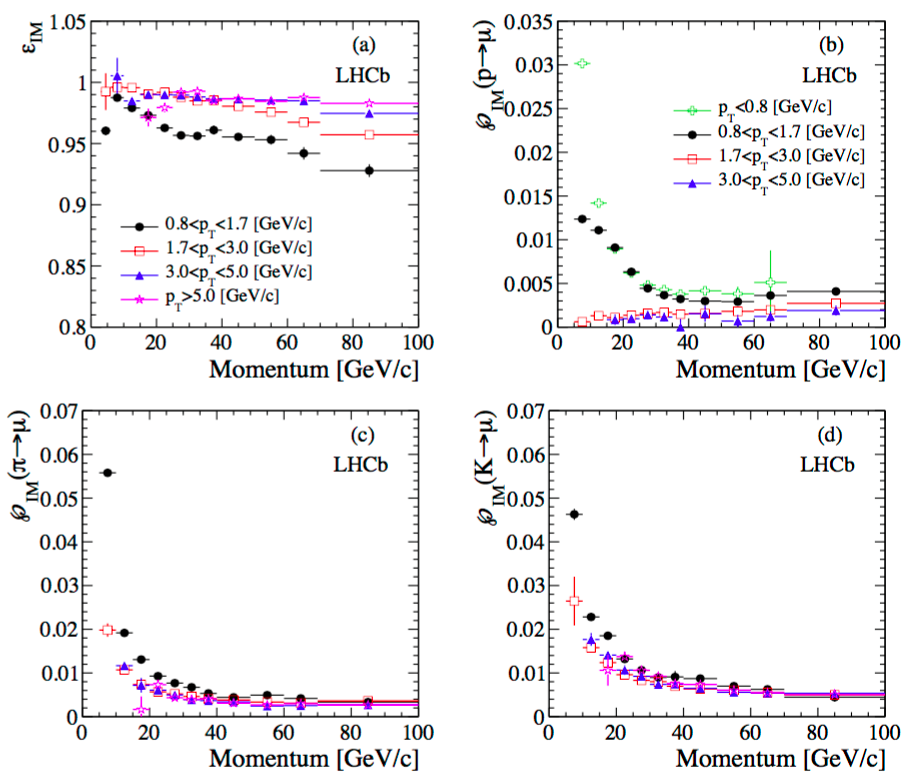
\includegraphics[width=1.0\textwidth]{./Figs/LHC_LHCb/isMuon_eff.png}
  \caption{Muon efficiency (top left) and misidentification probabilities for protons (top right), pions (bottom left) and kaons (bottom right) for isMuon criteria \cite{Archilli:2013npa}. }
  \label{fig:isMuon_efficiency}
\end{figure}




The information from all the PID detectors is combined using two different methods to provide global particle identification variables. One method is based on likelihood fits and the other is based on Neural Networks. In the first method, likelihood fits are performed in each sub-detector comparing each charged particle track to different particle hypotheses. The information from the likelihood fits in each sub detector are combined into a global variable. The final variable is the difference in the log-likelihoods between the track corresponding to a pion and a different particles hypothesis (kaon, proton, muon, electron), giving a measure of how likely each particle hypothesis is compared to that of a pion. These variables are known as DLL variables where the difference in log-likelihoods between the track corresponding to a pion and a kaon would be given by DLL$_{K\pi}$.




The second method uses information from the PID detectors and the tracking system in Neural Networks to provide a global probability of a track having a particular particle hypothesis. This method takes into account correlations between detector systems and extra detector information that are not considered in the likelihood method. The Neural Networks are trained on simulated inclusive $b$ decays and can be tuned to suit different situations, such as the data taking year. The variables produced by the Neural Networks are known as ProbNN variables where the probabilty of a particle being a muon is given by ProbNN$\mu$ and the probabilty of a particle being a pion is given by ProbNN$\pi$.


Figure~\ref{fig:DLL_vs_ProbNN} shows a comparison of the performance of the DLL and ProbNN variables in selecting protons and muons. Although the performance to the two types of variables are quite different, the efficiencies of each variable varies with different kinematic properties of the decay. The most appropriate PID variable type to use depends on the physics analysis it is being used in. 




\begin{figure}[htb] 
  \centering    
  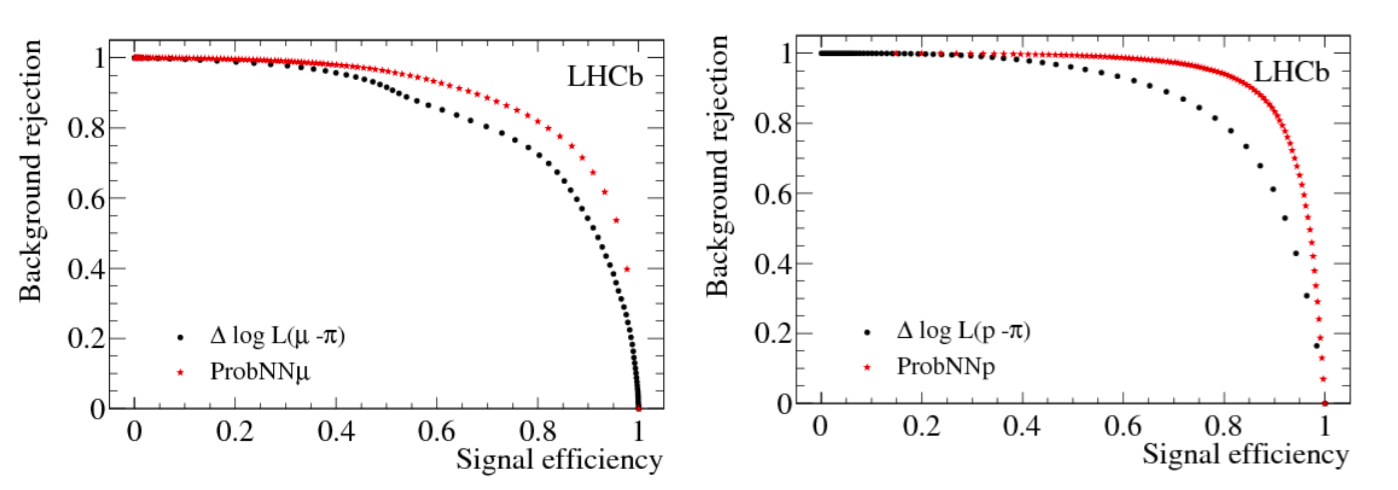
\includegraphics[ width=1.0\textwidth]{./Figs/LHC_LHCb/DLL_vs_ProbNN.png}
  \caption{Muon (left) and proton (right) signal efficiency vs background rejection for DLL and ProbNN PID variables \cite{Alves:2008zz}.}
  \label{fig:DLL_vs_ProbNN}
\end{figure}







\subsection{Trigger}

\label{Trigger}

The LHC was designed to collide protons at a rate of 40 MHz, this rate is too high for information to be read out of the LHCb detector. However most $pp$ collisions do not produce particles within the detector acceptance that are interesting for physics analyses at LHCb. A trigger system is used to identify $pp$ collisions that contain potentially interesting physics processes, the information from these events are saved for later use in physics analyses. The trigger has been designed to select interesting physics events with a high efficiency whilst reducing the event rate to one where information from the full detector can be read out.  There are two levels to the LHCb trigger; the hardware trigger and the software trigger. The hardware trigger is know as the level-zero (L0) trigger and reduces the 40~MHz collision rate to 1~MHz at which the full detector can be read out. The software trigger is know as the High-Level-Trigger (HLT), it has two stages and runs on the output of the L0 further reducing the event rate by utilising information for all the detector sub-systems. Each level of the trigger is composed of trigger `lines'; these lines are made up of reconstruction and selection algorithms and either accept or reject each event. Only events that are acceptance by a trigger line at both the L0 and HLT are available for use in physics analyses. 

\subsubsection{L0 trigger}
\label{L0}


The L0 trigger runs synchronously to the LHC bunch crossing. Its purpose is to reduce the events rate to 1~MHz, where information from the full detector can be read out. Therefore the L0 is limited to use information from the detector that can be read at the same rate as the LHC collision rate.
The L0 uses information from 3 parts of the detector, the VELO, calorimeters and the muon stations, to make decisions about the relevance of each event.%; the VELO, calorimeters and the muon stations. 


The pileup veto stations in the VELO are used in L0 pileup trigger lines, these lines identity the number of collisions in an event and are predominatley used for luminosity measurements~\cite{Aaij:2011er}.

The other L0 trigger lines are based on the kinematic properties of \bhadron decays. The heavy masses of \bhadrons means that their decays are characterised by the production of daughter particles with large transverse momentum ($p_{T}$) and transverse energy ($E_{T}$).
%The calorimeters are used to identify events that conating electrons, photons and hadrons with high $E_{T}$. 
The calorimeters are used in trigger lines that select events containing high $E_{T}$ electrons, photons or hadrons. Information from the PS, SPD, ECAL and HCAL is used to identify electrons, photons and hadrons in each event. Events are then accepted by the trigger lines if there is an electron, photon or hadron with $E_{T}$ above a threshold value provided the event multiplicity is not too high. The $E_{T}$ thresholds are different for each particle type. Events with high multiplicity take a long time to reconstruct and process in the HLT, therefore it is not efficiency to keep these events. The multiplicity is measured by the number of hits in the SPD detector (nSPD), only events with nSPD lower than a specified value can pass an L0 trigger line. 


In a similar way to the calorimeters, the muon stations are used to identify muons with high $p_{T}$ for trigger lines. There are two L0 trigger lines for muons that accept events based on muon $p_{T}$ if either a single muon has a $p_{T}$ above a threshold value or if the two muons with this highest $p_{T}$ have $\sqrt{p_{T1} \times p_{T2}}$ above a threshold value, provided the event multiplicity is not too high. %The L0 muon trigger lines are most important to select \bsmumu candidates. The efficiencies for these 2 lines are show in Figure X, most events are triggered by the L0Muon but some are added by the L0Dimuon lines. 

The $E_{T}$ and $p_{T}$ thresholds and the multiplicity limit for the L0 trigger lines vary for each year of data taking depend on the bandwidth available for the trigger. % and are shown in table X. 


\subsubsection{HLT trigger}
\label{HLT}

Events that are accepted by trigger lines in the L0 are moved to the Event Filter Farm where the HLT is run. The HLT is a software trigger that is split into two levels that are run successively. During the long shut down between Run~1 and Run~2 of the LHC significant changes were made to the reconstruction of particle decays used to make decisions within the HLT. 


The HLT1 is the first level of the HLT. It runs on the output of the L0 checking the decisions make by the L0 trigger lines and reducing the event rate. % from 1 MHz for processing in the HLT2. 
The HLT1 trigger lines are composed of generic selection criteria, making decisions that confirm those made in the L0 about particular particle types and also identify generic types of particle decays such as inclusive \bhadron decays. 
The second level of the HLT, the HLT2, runs on the output of the HLT1 trigger and consists of trigger lines designed to select decays relevant to specific physics analyses or particle decay topologies.




During Run~1 time constraints in the HLT1 trigger to process the output of the L0 did not allow for full event reconstruction using all LHCb sub-detectors, instead the HLT1 ran reconstruction and selection algorithms on event information only from the VELO and tracking stations. The reduced output of the HLT1 then provided an event rate that was low enough to allow event reconstruction that includes all detector subsystems to be used in the HLT2. However the reconstruction used in the HLT2 was different to the offline reconstruction that is used in physics analyses. Significant changes were made in the reconstruction used in the HLT between Run 1 and Run 2, the details of the changes made can be found in \cite{Lupton:2230910}. The majority of the changes to the HLT for Run 2 are not relevant for the analysis discussed in this dissertation, but the overall change is that the same reconstruction is used in the HLT and the offline reconstruction. 

%These trigger lines are composed of generic selection criteria, making decisions that confirm those made in the L0 about particular particle types and also identify generic types of particle decays such as inclusive \bhadron decays. The second level of the HLT, HLT2, runs on the output of the HLT1 which provides an event rate that is low enough to allow event reconstruction that includes all detector subsystems. The trigger lines in the HLT2 are designed to select decays relevant to specific physics analyses or particle decay topologies, this is made possible by detailed information from the reconstruction. 

Just like the L0 trigger, trigger lines in the HLT vary for each year of data taking both the selection criteria used in the lines and also new trigger lines are introduced. The number of HLT2 lines increases with each year of data taking as understanding of the capabilities of the experiment increases; there were about 100 HTL2 lines in 2011, 200 in 2012 and 450 in 2015. 

%\subsubsection{Trigger decisions}
%\label{trigger_decisions}
%The trigger lines in the L0 and HLT return three different types of decisions that are used to classify events. The choice of which type of trigger decision to use depends on the particular physics analysis and the signal decay of interest, the decisions can either be used line by line or as global decisions taking all lines together. The different decisions are:
%\begin{itemize}
%\item {\bf TOS}, `triggered on signal', tracks and hits that make up signal candidate of a physics analysis are sufficient for the event to pass the trigger line. 
%\item {\bf TIS}, `triggered independant of signal', if the tracks and hits associated with the signal candidate of a physics analysis are removed from the event, other tracks and hits would still cause the event to pass the trigger line.
%\item {\bf Dec}, refers to whether the event was accepted by the trigger line.
%\end{itemize}

\subsection{Software and simulation}
\label{SoftwareSimulation}
%Options instead of referenes, Susan references the realease areas!

The data that is read out of the LHCb experiment needs further processing before it can be used in physics analyses. The \textsc{Gaudi} framework~\cite{Mato:1998gfa} is a C++ framework that is the basis for the software applications needed to process the data at LHCb~\cite{Antunes-Nobrega:835156}. This framework ensures that the necessary software is available to all users and changes to the software are implemented across all applications, it is suited to the distributed computing system used in LHCb~\cite{Stagni:2012rs}. 


Once events have been accepted by the trigger, the first step in processing the output of the detector is reconstructing events, this is done by the \textsc{Brunel} application. It takes the digitised detector read out and reconstructs hits in the tracking stations to find particle trajectories and momenta and combines information from the RICH detectors, calorimeters and muon stations to compute PID variables. The output of processing by the \textsc{Brunel} application are stored in `Data Summary Type' (DST) files. 

Next the \textsc{DaVinci} application is used to fit the tracks reconstructed in \textsc{Brunel} with primary and secondary vertices. This application assigns particle hypotheses to each track and reconstructs the decay trees of particles in the detector, computing the kinematic properties that are needed for physics analyses. The the reconstructed output of the trigger is too large to be stored in one place and to be used by all analysts, therefore a `stripping' procedure is used to break up the data into a manageable size for  each physics analysis. Each physics analysis designs a set of loose selection requirements, called stripping lines, specific to their decays of interest, the selections are applied centrally to the reconstructed events and are designed to keep as much of the signal relevant to the analysis as possible but reduce the number background events. Only events that pass a stripping line selection are avaliable to be used in physics analyses. The output of this process are smaller DST files, events passing the stripping selections can either be saved with the full event information or with just the tracks related to the signal candidate. The choice depends on the physics process the stripping line is relevant for. The stripping selection is run a limited number of times and is applied seperately to data collected in different years. Requirements are imposed on the amount of data each stripping line can retain, typically the output of a line must be less than 0.05~$\%$ of the original data set size if the full event information is saved. Each analyst then uses the DaVinci application one last time to produce \textsc{Root}~\cite{Brun:1997pa} files from the output of their stripping lines, these files display the data in histograms and are used for physics analyses. %RooFit has citation \cite{Verkerke:2003ir}


As well as data collected by the experiment, simulated data that mirrors what is expected in the experiment is needed to understand the detector performance and for physics analyses. There is a set of software applications that are dedicated to the production of Monte Carlo simulated events within the \textsc{Gaudi} framework. Events are generated using the \textsc{Gauss} application~\cite{1742-6596-331-3-032047, Clemencic:2011zza}, this package uses \textsc{Pythia}~\cite{Sjostrand:2006za,Sjostrand:2007gs} to model $pp$ collisions and the production of particles, then the \textsc{Evt}\textsc{Gen}~\cite{Lange:2001uf} application to calculate the decays of these particles. Final state radiation is modelled using \textsc{Photos}~\cite{Golonka:2005pn}. Both \textsc{Pythia} and \textsc{Evt}\textsc{Gen} have been tuned for the production and decay of particles within the LHCb detector. The \textsc{Geant4}~\cite{Agostinelli:2002hh,Allison:2006ve} toolkit is used to model the interaction of particles as the travel through the LHCb sub-detectors and the hits made by particles in the detector. In the simulation the type of particles generated and how they decay can be specified so that the simulated events are relevant to particular physics decays. The \textsc{Boole} application then produces the digitised detector read out based on the information from \textsc{Geant4} that mimics the detector read out when data is recored. The output of \textsc{Boole} encompasses the detector response to the different hits, the electronic read out and the L0 hardware trigger as well as including additional hits from event spillover and LHC backgrounds. The digitised response of the detector is then processed by \textsc{Brunel} and \textsc{DaVinci} in the same way as the real data to produce \textsc{Root} files that are used in physics analyses. %RooFit has citation \cite{Verkerke:2003ir}

The LHCb software framework is set up so that it can be used on the Worldwide LHC Computing Grid~\cite{Bird:2011zz, WWCG}, the Grid is made up of computers across the world that each store part for the LHCb data set and simulation data. Despite the stripping process the data produced at LHCb is too large to be stored in one place. The \textsc{Dirac}~\cite{Paterson:1397926} system manages grid sites and the \textsc{Ganga} project allows the submission analysis code to different grid sites. The grid enables analysts to process and study the large amounts of data produced by LHCb without having to store the data where the analyst is. 





\section{Summary}
\label{LHCb_data}
%Need to find some references for the future projections I suppose. 
%The LHCb experiment is one of 7 experiments that studies the products of $pp$ collisions created by the LHC. 

The data taking periods of the LHC can be split up into different `Runs' which are separated by Long Shut Down periods when maintenance and upgrades are performed on the LHC, the detectors and the accelerator chain that delivers protons to the LHC. Run 1 began in 2010 and ended in 2013, during this Run the LHC operated at two different centre-of-mass energies. In 2010 and 2011 the LHC delivered proton collisions a a centre-of-mass energy of 7~\tev, this was increased to 8~\tev in 2012. The luminosity recored by LHCb in each was; 0.04~\fb in 2010, 1.10~\fb in 2011 and 2.08~\fb in 2012. After Run~1 the LHC entered the Long Shutdown~1 (LS1) when the machine and experiments were prepared to deliver and detect proton collisions at $\sqrt{s}$~=~13. Run~2 began in early 2015 and is still on going, so far LHCb has recorded 0.32~\fb in 2015 and 1.67~\fb in 2016 both at a centre-of-mass energy of 13 TeV. Figure~\ref{fig:LHCb_lumi} shows the integrated luminosity collected by LHCb in each year of data taking. The recorded luminosity of Run~2 is currently less that what was recorded in Run~1, however the production cross section for \bhadrons approximately doubled with the increase in centre-of-mass energy between Run~1 and Run~2 therefore the Run~2 data set will already contain more \bhadrons useful for physics analyses than the Run~1 data set. 


The expected end of Run~2 is 2018 by which time LHCb is expected to have recorded 5~\fb luminosity during the Run. Run~2 will be followed by a second long shut down period (LS2) in which LHCb shall be upgraded ready to record proton collisions at 14~\tev during Run~3. This run of data taking is expected to be from 2021 - 2024 and by the end of Run~3 LHCb is expected to have collected an integrated luminosity of 23~\fb over all the runs. 

The physics analysis described in this thesis uses the full data sets from Run~1 and 2015 and data taken up to September during 2016. The 2016 data set is therefore reduced to 1.1~\fb.

\begin{figure}[htb] 
  \centering    
  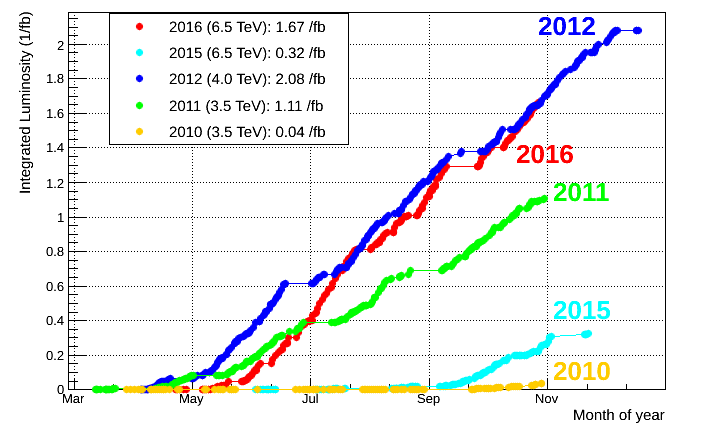
\includegraphics[ width=0.8\textwidth]{./Figs/LHC_LHCb/IntLumiRun1-2.png}
  \caption{Integrated luminosity collected by the LHCb experiment in each year of data taking. Source: LHCb.}
  \label{fig:LHCb_lumi}
\end{figure}

%In Run 1 LHCb ran at an instantaneous luminoscity of 3.5x10^32 cm-2s-1 whereas it was designed to run at 2.0x10^32 cm-2s-1. (Performance paper)

%\begin{figure}[htb] 
%  \centering    
%  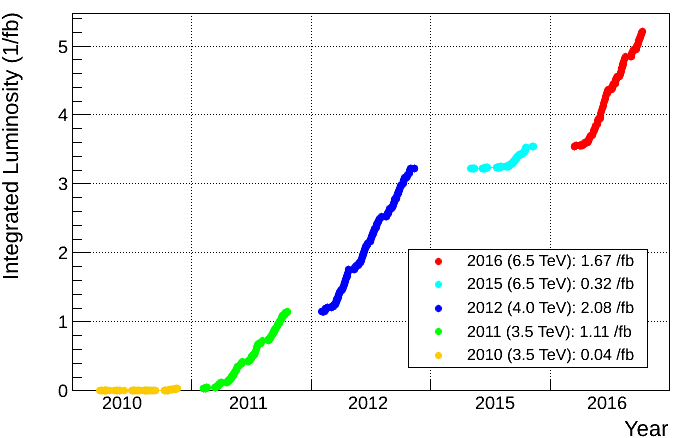
\includegraphics[ width=0.8\textwidth]{./Figs/LHC_LHCb/IntegratedLumiCumul.png}
%  \caption{Cumulative integrated luminosity collected over data taking years at the LHCb experiment. Source: LHCb.}
%  \label{fig:LHCb_lumi_cuml}
%\end{figure}



%To get a sideways table with wrapped text there are 2 options
%1. \begin{sideways} Content to rotate. \end{sideways}
%2. \afterpage{ \begin{landscape} Content to rotate. \end{landscape}
%Use afterimage for now.


\chapter{Selection of \bsmumu and \bhh decays}
\label{selection_chapter}


The analysis described in Chapter X for the \bsmumu effective lifetime requires \bsmumu and \bhh decays to be identified in the data sets recorded by the LHCb experiment. \bhh decays, where $h = K, \pi$, are used To understand different aspects of the selection and analysis of \bsmumu decays because they have large branching fractions, a similar topology to \bsmumu decays and are well understood from previous LHCb analyses. Although \bsmumu decays leave a clear 2 muon signature in the detector, the selection of these decays is challenging because it is a very rare process and there are many other processes (Sect.~\ref{sec:backgroundoutline}) that can mimic a \bsmumu decay in the detector. This Chapter describes the selection of \bmumu and \bhh decays for the measurement of the \bsmumu effective lifetime (Chapter~\ref{}), much of the selection is shared with the \bmumu Branching Fraction analysis(Chapter~\ref{}). The selection occurs in several stages and the development of the selection relies on simulated events (Sect.~\ref{sec:MCsamples}). The first step to select \bsmumu and \bhh decays is choosing what requirements to place on the trigger (Sect.~\ref{sec:triggerRequirements}) which is followed by a cut based selection to remove obvious background events (Sect.~\ref{sec:cutbasedsel}. Then particle identification variables (Sect.~\ref{sec:PID}) to reduced background events from mis-identified semi-leptonic and \bhh decays and finally multivariate classifiers (Sect.~\ref{sec:GeneralBDT}) are used as the last step in the selection to reduced the backgrounds to a low enough level so that the \bsmumu effective lifetime can be measured from the data. 

The LHCb collaboration has published a number of papers studying the \bsmumu decay, the selection described in this Chapter has been built up over a number of years by a range of different collaboration members. The selection detailed in Sections \ref{strippingstudies}, \ref{sec:PID} and \ref{sec:globalBDToptimisation} were completed for this thesis as well as all Figures and quoted efficiencies.


\section{Backgrounds}
\label{sec:backgroundoutline}
%A \bs decaying into two muons leaves information in the LHCb detector with certain identifying characteristics. The two muons form a good vertex that is displaced from the primary vertex of the event because the Bs has a long lifetime and the combined momentum of the muons can be extrapolated backwards to the primary vertex because the muons are the only decay products of the \bs. There are other processes that occur in proton-proton decays that can leave information in the detector in a similar pattern to \bsmumu decays. The reconstruction, described in Section X, produces many \bsmumu candidates, the aim of the selection is to separate the real \bsmumu decays from the background in the reconstructed candidates.

%The background sources for \bsmumu decays can be split into two groups, those that have quite obvious difference from \bsmumu decays and those that do not. The first set can be removed from the data set by taking advantage of the obvious differences whilst keeping a high 

The reconstruction process (Sect.~\ref{SoftwareSimulation}) produces numerous \bsmumu candidates from pairs of muons created during $pp$ collisions. Some candidates will have come from real \bsmumu decays but there are other background processes that occur during $pp$ collisions which leave a signature in the detector that can be reconstructed incorrectly as a \bsmumu decay. %In the detector a \bsmumu decay will produce two muons that form a good vertex which is displaced from the primary vertex where the \bs was produced.   
he selection aims to separate real \bsmumu decays from the background to produce a set of \bsmumu candidates with a high signal purity fro\
m which the \bs effective lifetime can be measured.
%The selection aims to seperate real \bsmumu decyas from these background to produce a set of \bsmumu candidates with a high signal purity from which the \bs effective lifetime can be measured. (here?)
%The main sources of background processes for \bsmumu decays are;
The main background sources that mimic \bsmumu decays are:
\begin{itemize}
\item Elastic collisions of protons that produce a pair of muons via the exchange of a photon, $pp \to p \mu^{+} \mu^{-} p$. The protons travel down the beam pipe and are undetected leaving the muons to be reconstructed as \bsmumu. Typically the muons produced in this way have low transverse momentum. %whilst the protons travel down the beam pipe. The muons produced have low transverse momentum.
\item Inelastic proton collisions that create two muons at the primary vertex. The muons form a good vertex and can be combined to for a \bs that decays instantaneously. This type of background is prompt combinatorial background. 
\item $B_{}^{0}\to\mu^{+}\mu^{-}\gamma$ decays where the photon is not reconstructed. The presence of the photon in the decay means that $B_{S}^{0}\to\mu^{+}\mu^{-}\gamma$ decays are not helicity suppressed and could therefore be a sizable background, however the photon gains a large transverse momentum resulting in the reconstructed \bs mass being much lower than expected.
\item Random combinations of muons produced by separate semi-leptonic decays. The \bsmumu candidates formed in this way are long lived combinatorial background because the reconstructed \bs will not decay instantaneously. %The mass distribution of this background is either an exponetially decaying slope or a flat distribution as illustrated in Figure~\ref{fig:LHCbCMS}. %can be formed when muons produced in separated semi-leptonic decays are combined. These are known as long lived combinatorial background because the reconstructed \bs will not decay instantaneously.
\item Semi-leptonic decays where one of the decay products is mis-identified as a muon and/or is not detected. The resulting mass of the \bs candidate is lower than expected due to the missing particle information. The semi-leptonic decays that contribute to \bsmumu backgrounds in this way are \bdpimunu, \bsKmunu, \bpimumu, \bdpimumu and \bcjpsimunu where \jpsimumu. %The mass distribution of these backgrounds are illustrates in Figure~\ref{fig:LHCbCMS} as the semi-leptonic decays.
\item \bhh decays, where $ h  = K, \pi$, when both hadrons are mis-identified as muons. This usually occurs when the hadrons decay whilst travelling through the detector. Similarly to mis-identified semi-leptonic decays the reconstructed \bs candidate mass is lower than expected. %The mass distribution of these backgrounds are illustrates in Figure~\ref{fig:LHCbCMS} as peaking backgrounds.
\item \bdmumu decays that are identical to \bsmumu decays apart from the difference in the $B$ meson masses. The \bd decay is irrelevant for the measurement of the \bsmumu effective lifetime and is therefore a background for this measurement.
\end{itemize}

%The selection aims to separate real \bsmumu decays from the background to produce a set of \bsmumu candidates with a high signal purity from which the \bs effective lifetime can be measured. 
The separation of \bsmumu decays from the backgrounds is challenging because \bsmumu decays are highly suppressed decays therefore reconstructed candidates are predominately made from background decays.
The removal of some background decays is straight forward by taking advantage of obvious differences between the \bsmumu and the backgrounds, however background from mis-identified semi-leptonic and \bhh decays and long lived combinatorial background are difficult to remove. The dimuon invariant mass distribution from the last published \bmumu Branching Fraction analysis but LHCb is shown in Figure~\ref{fig:LHCbCMS}, components for background from mis-identified semi-leptonic and \bhh decays are present below the \bs mass and the long lived combinatorial background has an almost flat distribution across the entire mass range. 
%The \bdmumu is also a background process for measuring the \bsmumu effective lifetime, the only way to seperate \bsmumu and \bdmumu decays is by using the different masses of the \bs and $B^{0}$ mesons. (In the bullet points?)

%Maybe say how since the decay is so rare there are many many more reconstruced background decays than real bsmumu decays?

\begin{figure}[htbp]
    \centering
   % \begin{subfigure}[b]{0.4\textwidth}
        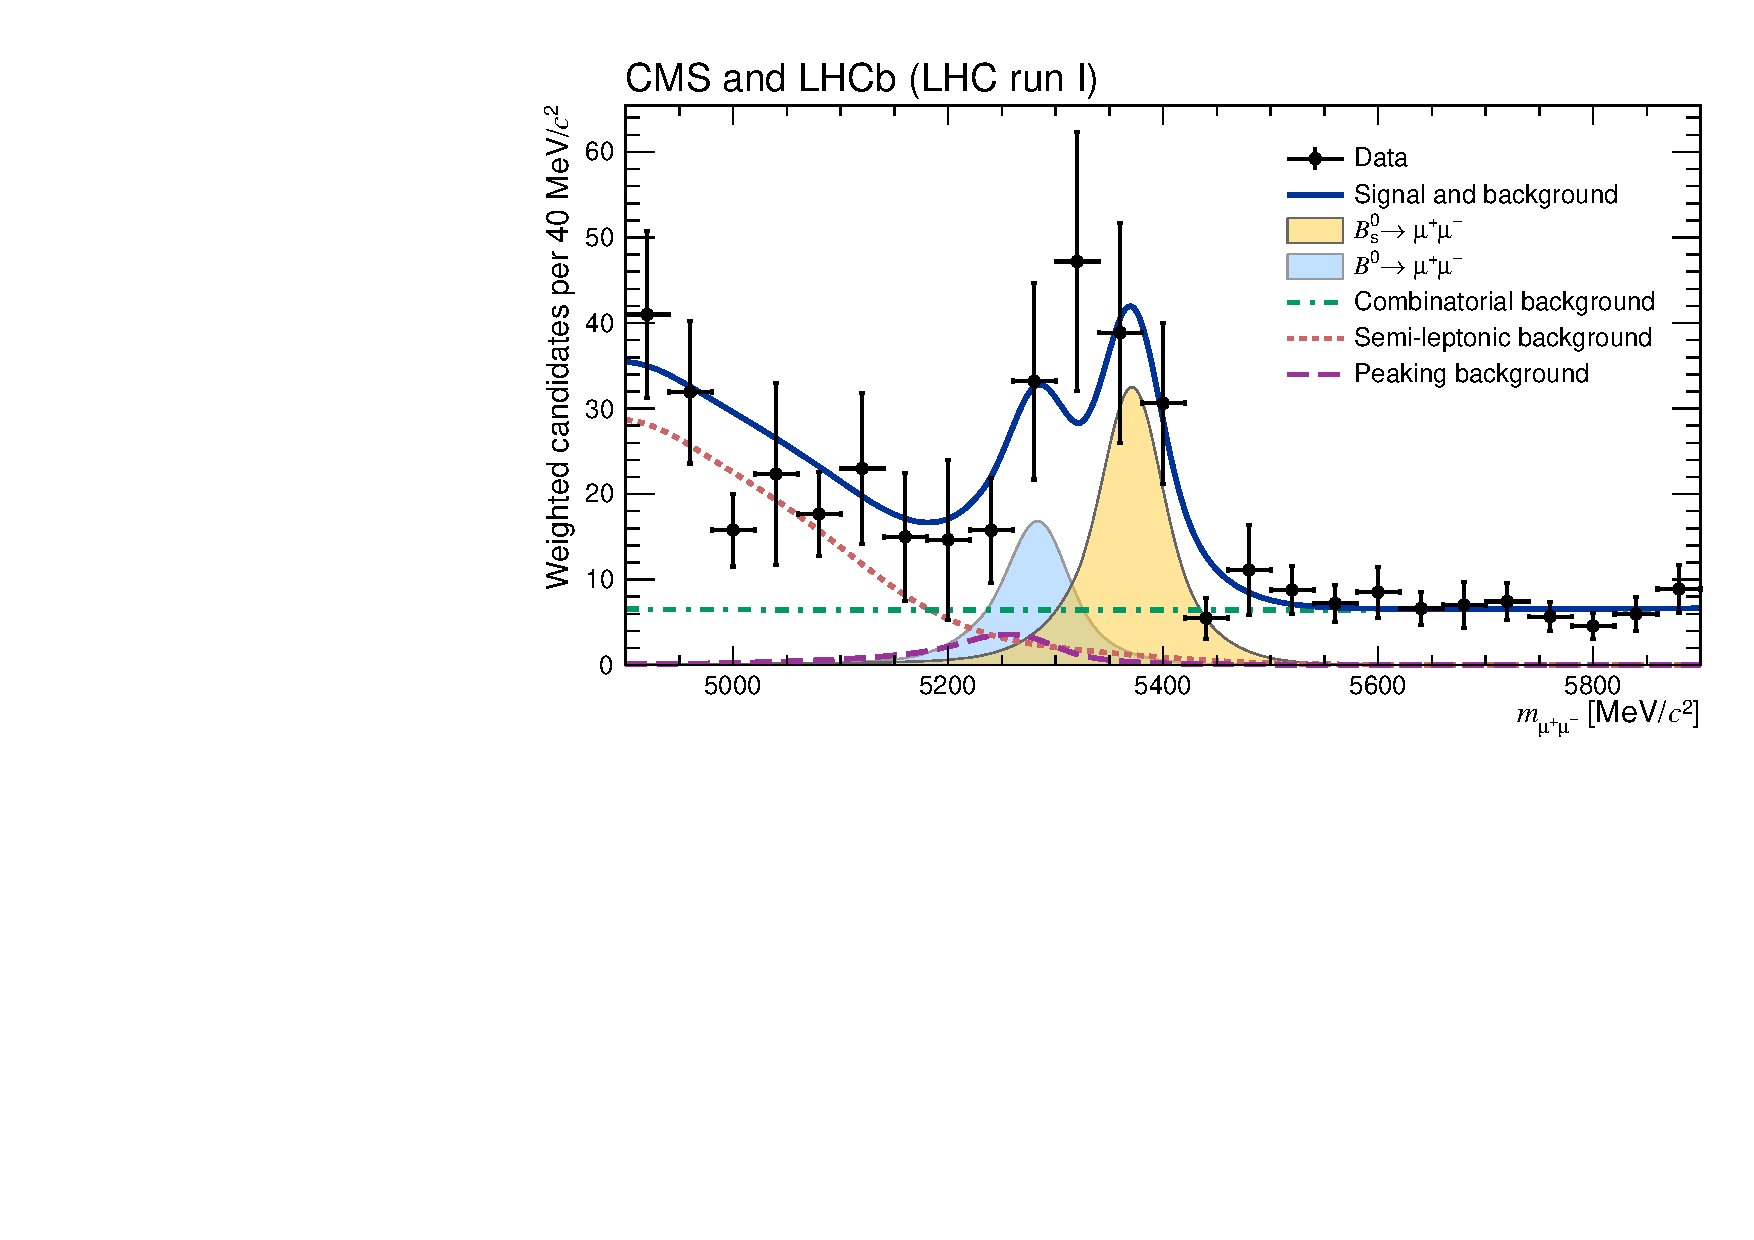
\includegraphics[width= 0.8 \textwidth]{./Figs/Selection/CMSLHCb_fig2.pdf}
        %\caption{ }
       % \label{fig:BDTSsig}
    %\end{subfigure}
   % ~ %add desired spacing between images, e. g. ~, \quad, \qquad, \hfill etc. 
      %(or a blank line to force the subfigure onto a new line)
   % \begin{subfigure}[b]{0.4\textwidth}
      % 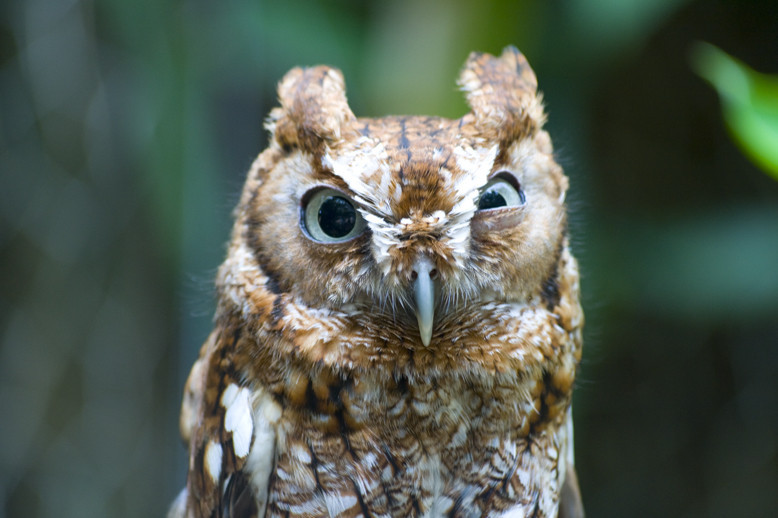
\includegraphics[width=\textwidth]{./Figs/placeholder.jpeg}
      %  \caption{ }
     %   \label{fig:BDTSbkg}
  %  \end{subfigure}
    \caption{Weighted dimuon invariant mass spectrum from combined analysis of CMS and LHCb Run~1 data for \bmumu Branching Fraction measurements~\cite{CMS:2014xfa}. Backgrounds included in the mass fit are mis-identified semi-leptonic decays in red, mis-identified \bhh decays in purple and long lived combinatorial background in green. }
    \label{fig:LHCbCMS}
\end{figure}

%{\it I could put a plot showing the mass plot from the previous analysis or I could make a plot something like Siim has to illustrate what i mean but that feels a bit like copying!}
%Separating the backgrounds from the \bsmumu decays can be done relatively straightly forwardly for many of the background processes by taking advantage of the obvious differences between the background and \bsmumu decays. However, distinguishing \bsmumu decays from long lived combinatorial backgrounds, and mis-idetificed \bhh and semi-leptonic decays is more challenging and \bsmumu decays must be sacrificed in order to remove a sufficient about of the background processes for the analysis to be performed. For the effective lifetime analysis the \bdmumu decay is not relevant and is therefore a background, however since the decays are extremely similar the \bsd masses are the only way to seperate the decays.

\section{Simulated Particle Decays}
\label{sec:MCsamples}
Simulated particle decays, as described in Section~\ref{SoftwareSimulation}, are used to develop the selection and analysis of \bsmumu decays. Large clean samples of simulated decays are needed to separate signal decays from background decays and to understand the impact of selection criteria on decays present in data. 
%Many different simulated decay types have been used over time for the development of the selection and analysis of \bsmumu decays, 
The simulated decays used for studies documented in this thesis are listed in Table~\ref{tab:MC_decays} along with the data taking conditions and simulation versions used to generated the decays.
\begin{table}[htbp]
\begin{center}
%%\begin{tabular}{p{6cm}p{2.5cm}p{2cm}p{3cm}}                                                                                                           
\begin{tabular}{p{0.45 \textwidth}p{0.15 \textwidth}p{0.15 \textwidth}p{0.15 \textwidth}}
\hline
Decay 			& Data taking conditions 	& Simulation version 	& Generated events \\ \hline 
\multicolumn{4}{c}{{\it Stripping selection studies selection}}  \\ \hline 
\bsmumu			& 2012	& sim06b  		& 2 M			 \\ 
\bdmumu			& 2012	& sim06b  		& 2 M\\ 
\bdkpi			& 2012	& sim06b  		& 1 M\\ 
\bujpsik		& 2012	& sim06b  		& 1 M\\ \hline 
\multicolumn{4}{c}{{\it Multivariate classifier training}}  \\ \hline
\bbbarmumux, {\footnotesize p~$>$~3~\gevc, 4.7~$< M_{\mu^{+} \mu^{-} <$~6.0~\gevcc, DOCA~$<$~0.4mm, 1~$<$~PtProd~$<$~16~\gevc}
                        & 2012  & sim06b                & 8.0 M      \\
\bbbarmumux, {\footnotesize p~$>$~3~\gevc, 4.7~$< M_{\mu^{+} \mu^{-} <$~6.0~\gevcc, DOCA~$<$~0.4mm,   PtProd~$>$~16~\gevc}
                        & 2012  & sim06b                & 6.6 M\\
\bsmumu                 & 2012  & sim06b                & 2 M \\ \hline
\multicolumn{4}{c}{{\it Analysis method development}}  \\ \hline 
\bsmumu			& 2011 	& sim08a   		& 0.6 M		  \\ 
       			& 2012 	& sim08i  		& 2 M			 \\ 
        		& 2015	& sim09a  		& 2 M	 \\ 
        		& 2016	& sim09a  		& 2 M ? \\ %Is this correct? I thought in the ntuples we have a lot more 2015 than 2016 MC? 
\bdkpi			& 2011	& sim08b  		& 0.8 M  \\ %11102003
        		& 2012	& sim08g  		& 8.6 M \\ 
        		& 2015	& sim09a  		& 4 M  \\ 
        		& 2016	& sim09a  	 	& 8.2 M \\ 
\bskk   		& 2012	& sim08g  		& 7.2 M \\ %13102002, 2016 is sim09a 4.1 M per pol, 2011 is sim-8b and 0.8 M per pol
        		& 2015	& sim09a   		& 4 M \\  \hline
\end{tabular}
\vspace{0.7cm}
\caption{Simulated decays used for developing the selection and the analysis of \bsmumu listed according to the studies the decays are used in. Cuts are applied to \bbbarmumux decays as they decays are generated, these cuts are included alongside the decay type and are applied to the muon momenta, invariant mass of the muons, the distance of closest approach of the muons and the product of the transverse momenta of the muons.}
\label{tab:MC_decays}
\end{center}
\end{table}

There exist multiple versions of the simulation because it is updated as understanding of the detector increases and to incorporate differences in data taking conditions, such as the trigger lines or center-of-mass energy, used each year of data is collected. Similar simulation versions must be used to compare different types of simulated decays or data taking conditions so that differences are not masked by variations in the simulation of the decays. The simulated decays in Table~\ref{tab:MC_decays} listed under the studies they are used in. 

Simulated \bbbarmumux decays are used to understand the combinatorial background of \bsmumu decays, however producing a large enough sample of these decays to be useful is computational expensive and produces large output files to save generated decays. Therefore cuts are applied at the generation level for \bbbarmumux decays to reduce the size of the samples that are saved and to speed production. The cuts, listed in Table~\ref{tab:MC_decays}, are applied on the muon momenta, the reconstructed mass of the muon pair, the product of the momenta of the muons and the distance of closest approach of the two muon. %The generator level cuts save a factor of 5 of what needs to be saved, striping filtering also reduces it by a factor of 10! The information is in the LHCb-ANA-2013-032, the 2012 bbbarmumux sample corresponds to 7fb-1.
  
%The development of the selection and analysis of \bsmumu decays requires the use of simuluated decays, as described in Section X. The reconstucted \bsmumu candidates come for a range of different different processes, as already discussed, in order to seperate real \bsmumu decays from the background, large clean samples of simulated decays are used so that the differences between signal and background decays can be understood. Futhermore simulated samples are needed to understand 

 


%Simulated \bsmumu, \bdmumu, \bdkpi and \bujpsik decays for 2012 data taking condition are used for studying the stripping selection in Section X.

%The training and testing of multivarite classifiers in Section X uses simulated \bsmumu and \bbbarmumux decays for for 2012 data taking conditions.
 
%Simulated events for \bsmumu, \bskk and \bdkpi for data taken in 2011, 2012, 2015 and 2016 are used for developing the analysis method in Chapter X. 

%The production of simulated events is constantly being developed as understanding of the detector increases and to include changes made for each data is recorded at theLHC. Therefore there exists a number of different simulation versions that can be used to simulate events.

%Each year data is collected at LHCb the conditions the experiment operates at and the proton collisions delivered by the LHC change. These changes include differences in the the selection used in the trigger for each year and increases in the centre of mass energy of proton collisions. 

%Therefore to understand data collected in different years simulated events from each year of data taking is needed, it is important to use similar simulation versions for each year so that the difference in the data taking conditions are not masked by differences in simulation versions. Simiarly for training multivarite classifiers consistent simulation versions are needed for the signal and background samples so that difference between signal and background distributions are not masked by differences in simulation versions.

%In general the stripping selections are applied to simulated events, however events that do not pass the stripping selection are still saved and can be used after reprocessing the simulated events. However simulation conditions can be set up so that events that do not pass the stripping selection are discarded and can never be used and also cuts can be applied on particles when they are generated before the detector response is simulated and the events are reconstructed. This is used when a very large same of simulated events needs to be generated in order to have a suitably large same of events reconstructed and is the case for the samples of \bbbarmumux simulated events.

%Two simulated samples of \bbbarmumux is used to understand the long lived combinatorial background and for the training of the multivariate classifier in Section \ref{sec:BDT}. For these samples events that did not pass the stripping selection have not been saved and requirements were applied to the generated events. 
%Simulated \bsmumu events with the same simulation version are also used for training the multivariate classifier to keep the simulation condition consistent.
On the whole simulated decays accurately model what occurs in data, however there are a couple of area where the simulation falls short of reality.
%Although in general simulated events accurately model what occurs in data there are several areas where this is not the case. 
The distributions of particle identification variables and properties of the underlying proton-proton collision, such as the number of tracks in an event, are not well modelled in the simulation. %Have I said what an event is?
The mis-modelling of particle identification variables can be corrected for using the PIDCalib package~\cite{} and simulated decays can be re-weighted using information from data to accurately model the under lying event, this re-weighting is described in Section~\ref{}. 


\section{Trigger}
\label{sec:triggerRequirements}

%The trigger is the first step in the selection process and the structure of the trigger is described in Section X. Since \bsmumu decays are very rare a broad set of trigger requirements is used in order to keep a high proportion of \bsmumu decay at this step of the selection. Specific trigger lines are not used in the selection but rather the combined results of a large selection of trigger lines at each level of the trigger. The combinations of trigger lines used are the L0Global, Hlt1Phys and Hlt2Phys triggers. The L0Global trigger combines all trigger lines present in the L0 trigger, it selects an event provided at least one L0 selects it and rejects an event if no L0 trigger selects it. The Hlt1Phys and Hlt2Phys triggers are very similar to the L0Global trigger except that decisions are based only trigger lines related to physics processes and HLT trigger lines used for calibration are excluded. 

%Different trigger decisions on these lines are used to select decays for the Branching Fraction and effective lifetime analyses. The Branching fraction selection imposed the loosest trigger requirements by requiring a event to pass the `Dec' decision at each trigger level as illustrated in set `A' of Table X. Trigger decisions are defined in Section X. The effective lifetime analysis has slightly more constrained trigger requirement, requiring an event passes either the `TIS' or `TOS' decision at each level of the trigger as illustrated in set `B' of Table X. The trigger choice for the effective lifetime is motivated by the determination of the acceptance function in Section X. 
%The selection criteria used in trigger lines and the specific lines included in the trigger change with each year of data taking, the dominant lines for triggering \bsmumu decays for each year are shown in Table~X. 

%Events are required to be either TIS, triggered independent of signal or TOS, triggered on signal, on the trigger lines used at each level of the trigger.
%The selection criteria used in trigger lines and the specific lines included in the trigger change with each year of data taking, the dominant lines for triggering \bsmumu decays for each year are shown in Table~X. 
%Slightly different trigger requirements are used to select \bhh decays used to develop and validate the effective lifetime analysis, the same broad trigger lines are used but the requirement on the output varies depending on the use of the \bhh events. The are two sets of trigger requirements, set `A' and `C', in Table~\ref{tab:triggers} are used to select \bhh decays, it will be made clear in later sections where \bhh decays are used which trigger requirements are imposed. 

The trigger (Sect.~\ref{Trigger}) is the first step in the selection, it selects events that could contain an interesting particle decays and these events are saved to be used in physics analyses. \bsmumu and \bhh candidates are reconstructed from events that have passed the trigger. For each candidate it is useful to know whether is was a component in that candidate that caused the event to be selected by a trigger line or if it was another part of the event. There are several different decisions that identify this;
\begin{itemize}
\item TOS, triggered on signal - a candidate is identified as TOS if only information from the candidate was enough to cause a trigger line to select the event
\item TIS, triggered independent of signal - a candidate is identified as TIS if part of the event independent of the candidate was enough to cause a trigger line to select the event
\item DEC - a candidate is identified as DEC if anything in the event caused a trigger line to select an event. This includes TIS and TOS decisions and also when a combination of information from the candidate and something else in the event caused a trigger line to select the event
\end{itemize}

\bsmumu decays are very rare decays and therefore trigger requirements used to select these decays are chosen to keep a high efficiency is kept at this step of the selection. The trigger lines L0Global, Hlt1Phys and Hlt2Phys are used and candidates are required to be TOS or TIS at each level of the trigger. These trigger lines combine the decisions of many individual lines used in the trigger which allows a high efficiency to be achieved for selecting \bsmumu decays. The L0Global trigger combines all trigger lines present in the L0 trigger, it selects an event provided at least one L0 trigger line selects it and rejects an event if no L0 trigger selects it. The Hlt1Phys and Hlt2Phys triggers are very similar to the L0Global trigger except that decisions are based only trigger lines related to physics processes and HLT trigger lines used for calibration are exclude.


Slightly different trigger decisions are used to select \bhh decays but the same trigger lines are used. To be useful as a validation channel the efficiency of the trigger requirements as a function of the decay time needs to be similar to the \bsmumu triggers, this is achieved by requiring \bhh decays to be TIS at each level of the trigger. %\bhh candidates are required to be TIS at each level of the trigger, this trigger decision is used to ensure the trigger efficiency to select \bhh decays is similar to the \bsmumu trigger efficiency. 

The requirements imposed on the trigger to select \bsmumu and \bhh decays is shown in Table~\ref{tab:triggers}.

\begin{table}[htbp]
\begin{center}
\begin{tabular}{ll}
\hline
Trigger Line	& Trigger decision \\ \hline
%\multicolumn{2}{c}{{\it set A}} \\ \hline
%L0Global	& Dec\\
%Hlt1Phys	& Dec \\
%Hlt2Phys	& Dec \\ \hline
\multicolumn{2}{c}{{\it Select \bsmumu decays}} \\ \hline
L0Global	& TIS or TOS \\
Hlt1Phys	& TIS or TOS \\
Hlt2Phys	& TIS or TOS \\ \hline
\multicolumn{2}{c}{{\it Select \bhh decays}} \\ \hline
L0Global	& TIS\\
Hlt1Phys	& TIS \\
Hlt2Phys	& TIS \\ \hline
\end{tabular}
\vspace{0.7cm}
\caption{Trigger lines used to select \bsmumu and \bhh decays.}% Set `A' is used to select decays for the Branching Fraction analysis. Set `B' is used to select \bsmumu decays for the effective lifetime analysis. Sets `A' and `C' are used to select \bhh decays used to develop the \bsmumu effective lifetime analysis.}
\label{tab:triggers}
\end{center}
\end{table}


%There was a problem with the implementation of the Hlt2Phys Dec decision in 2016 simulated events.%, the decision returned was always 1.  
%This only affect the selection of \bhh decays. In order to emulate this trigger a combination of Hlt2 lines that select \bhh events, listed in Table~\ref{tab:HltDecEmulation}, is used instead of HLT2Phys when the Dec decision is required. 

%\begin{table}[ht]
%\begin{center}
%\begin{tabular}{l}
%\hline
%\bhh trigger lines \\ \hline
%Hlt2Topo2BodyDecision Dec  \\
%Hlt2B2HH Lb2PPiDecision Dec \\
%Hlt2B2HH Lb2PKDecision Dec \\
%Hlt2B2HH B2PiPiDecision Dec \\
%Hlt2B2HH B2PiKDecision Dec \\
%Hlt2B2HH B2KKDecision Dec  \\
%Hlt2B2HH B2HHDecision Dec \\ \hline

%\end{tabular}
%\vspace{0.7cm}
%\caption{Trigger lines used to emulate the Hlt2Phys$\_$Dec decision for \bhh data and simulated events.}
%\label{tab:HltDecEmulation}
%\end{center}
%\end{table}

\section{Cut Based Selection}
\label{sec:cutbasedsel}
%http://lhcb-release-area.web.cern.ch/LHCb-release-area/DOC/stripping/config/stripping20/dimuon/strippingbs2mumulineswidemassline.html
The \bsmumu and \bhh candidates that pass the required trigger decisions are refined by a cut based selection. These selection cuts are aimed at removing obvious backgrounds by exploiting the differences between real \bsmumu decays and the backgrounds that mimic them. The selection of \bhh decays is kept as close as possible to that of \bsmumu decays. The cuts based selection is compared of two parts; the stripping selection and the offline selection. 

The stripping selection, as described in Section~\ref{Software_Simulation}, is applied to all events that pass the trigger. It consists of individual stripping lines that select reconstructed candidates for specific decays, the development of the stripping selection for \bsmumu and \bhh decays is described in Sections~\ref{strippingold}~and~\ref{strippingstudies}.% of stripping lines  by exploiting differences between the decays and the backgrounds that mimic them. 



%The selection of \bsmumu and \bhh decays for the \bsmumu effective lifetime measurement uses the same stripping lines as those in the \bmumu Branching Fraction measurements. These lines were designed at the start of Run~1 by studying the efficiencies of different selection cuts from simulated events \cite{}. However since then improvements have been made to the simulation of particle decays at LHCb, therefore it is prudent to check the accuracy of the selection efficiencies with updated simulated events and investigate where improvements can be made to the efficiency of the stripping selection used to select \bsmumu events. These studies are detailed in Sections~\ref{strippingold} and~\ref{strippingstudies}.

The offline selection cuts are applied to the output of the stripping selection. Overall stripping selection imposes loose selection requirements onto \bsmumu candidates so that as much information as possible is still available to develop the analysis and understand background events after the stripping selection. Therefore the offline selection further refines the data, removing background candidates. The full set of cuts applied in the stripping and offline selection to select \bsmumu and \bhh decays from Run~1 and Run~2 data are presented in Section~\ref{finalloosesel}. 


 
%REDO THIS AFTER WORKING OUT EXACTLY WHAT DETAILS I THINK ARE IMPORTANT TO INCLUDE!
%The stripping selection is a set of loose cuts that are applied to reconstructed events that have passed the trigger. The stripping selection consist of `lines' that are taylored to select particular decays. The aim of stripping lines is to reduce the size of the data sets collected by the experiment to a managable size on which tighter selection cuts to be developed and applied offline. Events that do not pass the selection cuts in the stripping lines are not directly avaliable to physics analyses. Therefore the cuts applied in the stripping lines are designed to remove obvious background events whilst keeping a high efficecny on the decay of interest. Restraints are placed on the amount of data that can pass the stripping selection for a particular analysis, typically this is set to be 0.05$\%$ of the original LHCb data set size for events that are saved in DST files. 
%This paragraph is ok.



\subsection{Development of the stripping selection}
\label{strippingold}

The stripping selection used to select \bsmumu and \bhh decays for the \bsmumu effective lifetime measurement uses the same stripping lines as the selection of \bmumu decays for the Branching Fraction measurement. The selection were designed at the start of Run~1 by studying the efficiencies of different selection cuts from simulated events~\cite{Diego}. However since then improvements have been made to the simulation of particle decays at LHCb, therefore it is prudent to check the accuracy of the selection efficiencies with updated simulated events and investigate where improvements can be made to the efficiency of the stripping selection used to select \bsmumu events.


In addition to \bmumu and \bhh decays the measurement of the \bmumu Branching Fractions requires \bujpsik decays. \bdkpi and \bujpsik decays are used to normalise the number of observed \bsmumu decays to the number created in $pp$ collisions. 

There are three stripping lines that select \bmumu, \bujpsik and \bhh candidates, the selection of the normalisation channels is kept as similar as possible to the signal selection to avoid introducing systematic uncertainties in the normalisation procedure of the branching fraction. However, the selection of \bujpsik decays must diverge from \bsmumu due to additional particles in the final state of the decay. Any changes made to the \bmumu stripping selection to improve the selection efficiency must be included in the selection to the normalisation channels to keep the systematic uncertainties under control, therefore all three stripping lines must be studied together. The stripping selection cuts applied for the Run~1 Branching Fraction analysis~\cite{CMS:2014xfa, Aaij:2013aka} to select \bmumu, \bhh and \bujpsik decays are listed in Table~\ref{tab:PreviousStripping}.


%The stripping selection cuts and cuts applied during the reconstruction of particle decays for the Run 1 \bmumu Branching Fraction analysis \cite{} to select \bmumu, \bhh and \bujpsik are shown in Table X. The selection of \bujpsik and \bhh decays is kept as similar as possible to the selection of \bsmumu decays to avoid introducing systematic errors when \bhh and \bujpsik decays are used in the normalisation for the Branching Fraction measurement. The selection of \bujpsik event must diverge from the \bsmumu selection due to additoinal particles in the final state of the decay. The stripping selection imposes more cuts to select \bhh decays compared to \bsmumu because \bhh decays are much more abundant therefore extra cuts are needed to reduce the number of events passing the stripping to an acceptable level. The cuts applied to \bhh in the stripping are the later applied to \bsmumu events after the stripping selection. 
%The measurement of the \bsmumu Branching Fraction, described in Chapter X, uses \bujpsik and \bdkpi decays to normalise the number of observed \bsmumu decays to the number created in proton-proton collisions. There are three stripping lines that select \bmumu, \bujpsik and \bhh candidates, where $h = K, \pi$, the selection of the normalisation channels is kept as similar as possible to the signal selection to avoid introducing systematic uncertainties in the normalisation procedure. However, the selection of \bujpsik decays must diverge from \bsmumu due to additional particles in the final state of the decay. Any changes made to the \bmumu stripping selection to improve the selection efficiency must be included in the selection to the normalisation channels to keep the systematic uncertainties under control, therefore all three stripping lines must be studied together. The stripping selection cuts applied for the Run~1 Branching Fraction analysis~\cite{} to select \bmumu, \bhh and \bujpsik decays are listed in Table~\ref{tab:PreviousStripping}.

\afterpage{
\begin{landscape}
%\vspace*{\fill}
\begin{table}[htbp]
\begin{center}
\begin{tabular}{l|lll}
\hline
  Particle              & \bsmumu                                     & \bhh                            &\bujpsik       \\
\hline             
\bs or $B^{+}$         & |M - M$_{PDG}$| $<$ 1200 \mevcc              & |M - M$_{PDG}$| $<$ 500 \mevcc    & |M - M$_{PDG}$| $<$   500 \mevcc   \\          
                      & DIRA > 0                                    & DIRA > 0                          & Vertex $\chi^{2}$/ndof < 45    \\       
                      & FD $\chi^{2}$ $>$225                        & FD $\chi^{2}$ $>$225             & IP $\chi^{2}$ $<$ 25  \\ 
                      & IP $\chi^{2}$ $<$ 25                         & IP $\chi^{2}$ $<$ 25              &         \\            
                      & Vertex $\chi^{2}$/ndof < 9                   & Vertex $\chi^{2}$/ndof < 9        &         \\   
                      & DOCA $<$ 0.3 mm                             & DOCA $<$ 0.3 mm                   &         \\               
                      &                                             & $\tau$ $<$ 13.248 \ps             &         \\
                      &                                             & $p_{T}$ $>$ 500 \mevc             &          \\
\hline   
\jpsi                  &                                             &                                   & |M - M$_{PDG}$| $<$   60 \mevcc   \\
                      &                                             &                                   & DIRA > 0    \\
                      &                                             &                                   & FD $\chi^{2}$ $>$ 225  \\
                      &                                             &                                   & Vertex $\chi^{2}$/ndof < 9        \\  
                      &                                             &                                   &   DOCA $<$ 0.3 mm       \\  
\hline             
Daughter $\mu$ or $h$   & Track $\chi^{2}$/ndof < 3                 & Track $\chi^{2}$/ndof < 3           & Track $\chi^{2}$/ndof < 3     \\       
                        & isMuon = True                             &                                    & isMuon = True           \\ 
                        & Minimum IP $\chi^{2}$ $>$ 25               & Minimum IP $\chi^{2}$ $>$ 25         & Minimum IP $\chi^{2}$ $>$ 25     \\                   
                        &    $p_{T}$ $>$ 0.25 \gevc                   & 0.25 \gevc $<$ $p_{T}$ $<$ 40 \gevc &  0.25 \gevc $<$ $p_{T}$ \\
%                        &                                           & $p$ < 350 \gevc                     &  \\
                        &                                           & ghost probability $<$ 0.3      &  \\
\hline
$K^{+}$                 &                                           &                                     & Track $\chi^{2}$/ndof < 3   \\
                       &                                           &                                     & $p_{T}$ $>$ 0.25 \gevc  \\
                       &                                           &                                     & Minimum IP $\chi^{2}$ $>$ 25 \\
\hline
\end{tabular}
\vspace{0.7cm}
\caption{Selection requirements applied during the stripping selection for Run~1 data used in the \bmumu Branching Fraction analysis~\cite{CMS:2014xfa, Aaij:2013aka} to select \bmumu, \bhh and \bujpsik decays. $M_{PDG}$ corresponds to the Particle Data Group~\cite{Olive:2016xmw} mass of each particle.}%The track $\chi^{2}$/ndof and isMuon cut are applied during the reconstruction.}
\label{tab:PreviousStripping}
\end{center}
\end{table}
%\vspace*{\fill}
\end{landscape}
}


The variables used in the stripping selection are:
\begin{itemize}
\item the reconstructed mass, $M$ - the mass and momenta of the decay products of the $B$ meson (or \jpsi) are combined to provide its reconstructed mass. Cuts on the mass remove candidates with a reconstructed mass far from the expected mass that are clearly backgrounds. Loose mass requirements are made on for the \bsmumu selection to allow for the study of semi-leptonic backgrounds that have a mass less than the \bs mass when mis-identified as \bsmumu decays;
\item the ``direction cosine'', DIRA - this is the cosine of the angle between the momentum vector of the particle and the vector connecting the production and decay vertices\footnote{The production vertex of the $B$ or the primary vertex is identified by extrapolating the $B$ meson momentum vector towards the beam axis. The closest vertex to the intersection of the $B$ momentum and the beam axis is assigned as the primary vertex.} of the particle. For correctly reconstructed candidates the direction cosine should be very close to one, requiring candidates to have positive value ensuring events are travelling in the incorrect direction are removed;
\item the flight distance (FD) \chisqd $ $- this is computed by performing the fit for the production vertex of a particle but including the tracks from its decay products that originate from the decay vertex in the fit as well. For a $B$ meson the FD \chisqd is likely to be large because $B$ mesons have long lifetimes therefore the tracks of its decays products will not point towards the production vertex;
\item track fit \chisqd/$ndof$ - provides a measure of the quality of a fitted track, placing an upper limit removes poor quality tracks and backgrounds composed of poorly reconstructed decays;
\item vertex fit \chisqd/$ndof$ - provides a measure of how well tracks can be combined to form a vertex, placing an upper limit removes poorly constrained vertices and backgrounds composed of poorly reconstructed decays;
\item distance of closest approach (DOCA) - this is the distance of closest approach of two particles computed from the straight tracks in the VELO. For the decay products of a particle, for example the muons from \bsmumu, this distance would ideally be zero because the muons originate from the same vertex;
\item decay time, $\tau$ - is the length of time a particle lives as it travels from its production vertex to its decay vertex. Applying an upper decay time cut removes unphysical background decays;
\item isMuon - particle identification variable defined in Section~\ref{PID} that returns True for muons and False for other particles;
\item transverse momentum, $p_{T}$ - the component of a particle's momentum perpendicular to the beam axis. Decay products of $B$ mesons are expected to have relatively high \pt due to the heavy $B$ meson masses however an upper limit removes unphysical backgrounds;
\item momentum, $p$ - an upper limit on the momentum of a particle  removes unphysical backgrounds;
\item ghost probability - defined in Section~\ref{Trackrecon} provides the probability of a tracking being composed on random hits in the detector, tracks from the passage of real particles will have a low ghost probability; 
\item impact parameter (IP) \chisqd $ $- this is the change in the fit for a primary vertex (PV) caused by removing one track in the fit. In a \bsmumu decay, the \bs is produced at the PV therefore it should have a small IP \chisqd value whereas the muons will be displaced from the PV because of the relatively long lifetime of the \bs and therefore will have a large IP \chisqd;
\item minimum impact parameter (IP) \chisqd $ $- this is the IP \chisqd of the muons with respect to all PVs in the event, this parameter is used to remove prompt muons created at any PV in the event and therefore reduce the prompt combinatorial background. 
\end{itemize}

The stripping selection imposes a greater number cuts to select \bhh decays compared to \bsmumu because \bhh decays are much more abundant therefore extra cuts are needed to reduce the number of events passing the stripping to an acceptable level. The cuts applied to only \bhh decays in the stripping are the later applied to \bsmumu candidates in the offline selection. %The cuts on muon transverse momentum, track \chisqd and isMuon (when used) are applied in the reconstruction and cannot be changed.


\subsection{Optimisation of \bsmumu stripping selection}
\label{strippingstudies}


The efficiency of the cuts used in the stripping lines to selecting \bmumu, \bhh and \bujpsik decays are shown in Table \ref{tab:Run1strippingEff}, only cuts that are in common with the \bmumu stripping lines are listed. The efficiencies are evaluated using 2012 sim06 simulated events that have the minimum track \pt, track \chisqd and isMuon requirements imposed. These cuts are applied during the reconstruction and particles that do not pass these requirements are not included in the samples of simulated decays. No trigger requirements have been applied so that only the effect of the stripping selection on the efficiencies can be assessed. During the simulation of particle decays the trigger is run in {/it pass through} mode so that all reconstructed are saved not just those that have passed a trigger line. 


\afterpage{
\begin{landscape}
\vspace*{\fill}
%\begin{sideways}
\begin{table}[htbp]
\begin{center}
\begin{tabular}{p{6cm}cccc}
                  & \multicolumn{3}{c}{Efficiency}  \\ 
\cline{2-5}
Requirement                                  & \bsmumu                   & \bdmumu                       & \bhh                &\bujpsik  \\
\hline
$B$ |M - M$_{PDG}$|                           & (100.00 $\pm$ 0.00)$\%$  & (100.00 $\pm$ 0.00 )$\%$      & (98.25 $\pm$ 0.02)$\%$        & (99.73 $\pm$ 0.02)$\%$ \\
\bsd or \jpsi DIRA                            & (99.41 $\pm$ 0.01) $\%$  & (99.47 $\pm$ 0.01)$\%$        & (99.47 $\pm$ 0.01)$\%$        & (95.83 $\pm$ 0.08)$\%$ \\
\bsd or \jpsi FD $\chi^{2}$                   & (83.74 $\pm$ 0.06) $\%$  & (83.96 $\pm$ 0.06)$\%$        & (83.83 $\pm$ 0.06)$\%$        & (82.90 $\pm$ 0.15)$\%$ \\
\bsd or \jpsi IP $\chi^{2}$                   & (96.78 $\pm$ 0.03) $\%$  & (96.93 $\pm$ 0.03)$\%$        & (97.44 $\pm$ 0.03)$\%$        & (97.52 $\pm$ 0.06)$\%$ \\
\bsd or \jpsi vertex $\chi^{2}$/ndof          & (97.21 $\pm$ 0.03) $\%$  & (97.18 $\pm$ 0.03)$\%$        & (97.68 $\pm$ 0.02)$\%$        & (96.78 $\pm$ 0.07)$\%$ \\
\bsd or \jpsi DOCA                           & (99.82 $\pm$ 0.01) $\%$   & (99.80 $\pm$ 0.01)$\%$        & (99.83 $\pm$ 0.01)$\%$        & (99.58 $\pm$ 0.03)$\%$ \\               

$\mu$, $h$, $K^{+}$ minimum IP $\chi^{2}$    & (80.16 $\pm$ 0.06) $\%$  & (80.62 $\pm$ 0.06 )$\%$        & (79.66 $\pm$ 0.07)$\%$        & (86.98 $\pm$ 0.14)$\%$ \\
\hline
Total after above cuts                  & (71.29 $\pm$  0.07) $\%$  & (71.82 $\pm$ 0.07)$\%$        & (70.97 $\pm$ 0.07)$\%$        & (71.30 $\pm$ 0.18)$\%$ \\
\hline
Total after all cuts      & -                         & -                             & (70.70 $\pm$ 0.07)$\%$        & (62.25 $\pm$ 0.20)$\%$ \\
\hline
\end{tabular}
\vspace{0.7cm}
\caption{Stripping line cut efficiencies for \bsmumu, \bhh and \bujpsik  2012 simulated decays. Selection cuts applied are listed in Table~\ref{tab:PreviousStripping}. Efficiencies have been calculated only for cuts that are present in the \bsmumu stripping, each cut separately and the total efficiencies are given for the listed cuts and the complete set of cuts present in each stripping line. }
\label{tab:Run1strippingEff}
\end{center}
\end{table}
\vspace*{\fill}
\end{landscape}
%\end{sideways}
}


The selection efficiencies are very similar for each stripping cut across the different decays which fits the requirement that the selection of signal and normalisation decays used in the branching fraction measurement are as similar as possible. The similarity of the selection efficiencies for the signal and normalisation decays is further illustrated in Figures~\ref{fig:ratioplotsJpsik} and \ref{fig:ratio_plotsBd2KPi} which show the ratio of selection efficiencies for \bsmumu decays to \bujpsik and \bdkpi decays for a range of selection cuts. With the exception of the \bsmumu and \bujpsik IP $\chi^{2}$ cuts on the daughter particles, the ratio of efficiencies is well within $3\%$ of~1 for the range of cuts values shown. The ratio of the \bsmumu and \bujpsik efficiencies for the daughter particle IP $\chi^{2}$ markedly deviates from unity, showing that the IP $\chi^{2}$ distribution of the muons and kaon are very different as seen previous in~\cite{Diego}. If the FD \chisqd, \bs or \jpsi IP \chisqd and vertex \chisqd selection cuts are applied to the simulated events before the daughter IP $\chi^{2}$ requirement the ratio of \bmumu and \bujpsik efficiencies is much closer to~1. The stability of the ratios of selection efficiencies across a large range of cuts values shows that changing a cut value in the \bmumu selection will have a similar impact on the efficiencies of the normalisation decays. 


\begin{figure}[htbp]
    \centering
    \begin{subfigure}[b]{0.4\textwidth}
        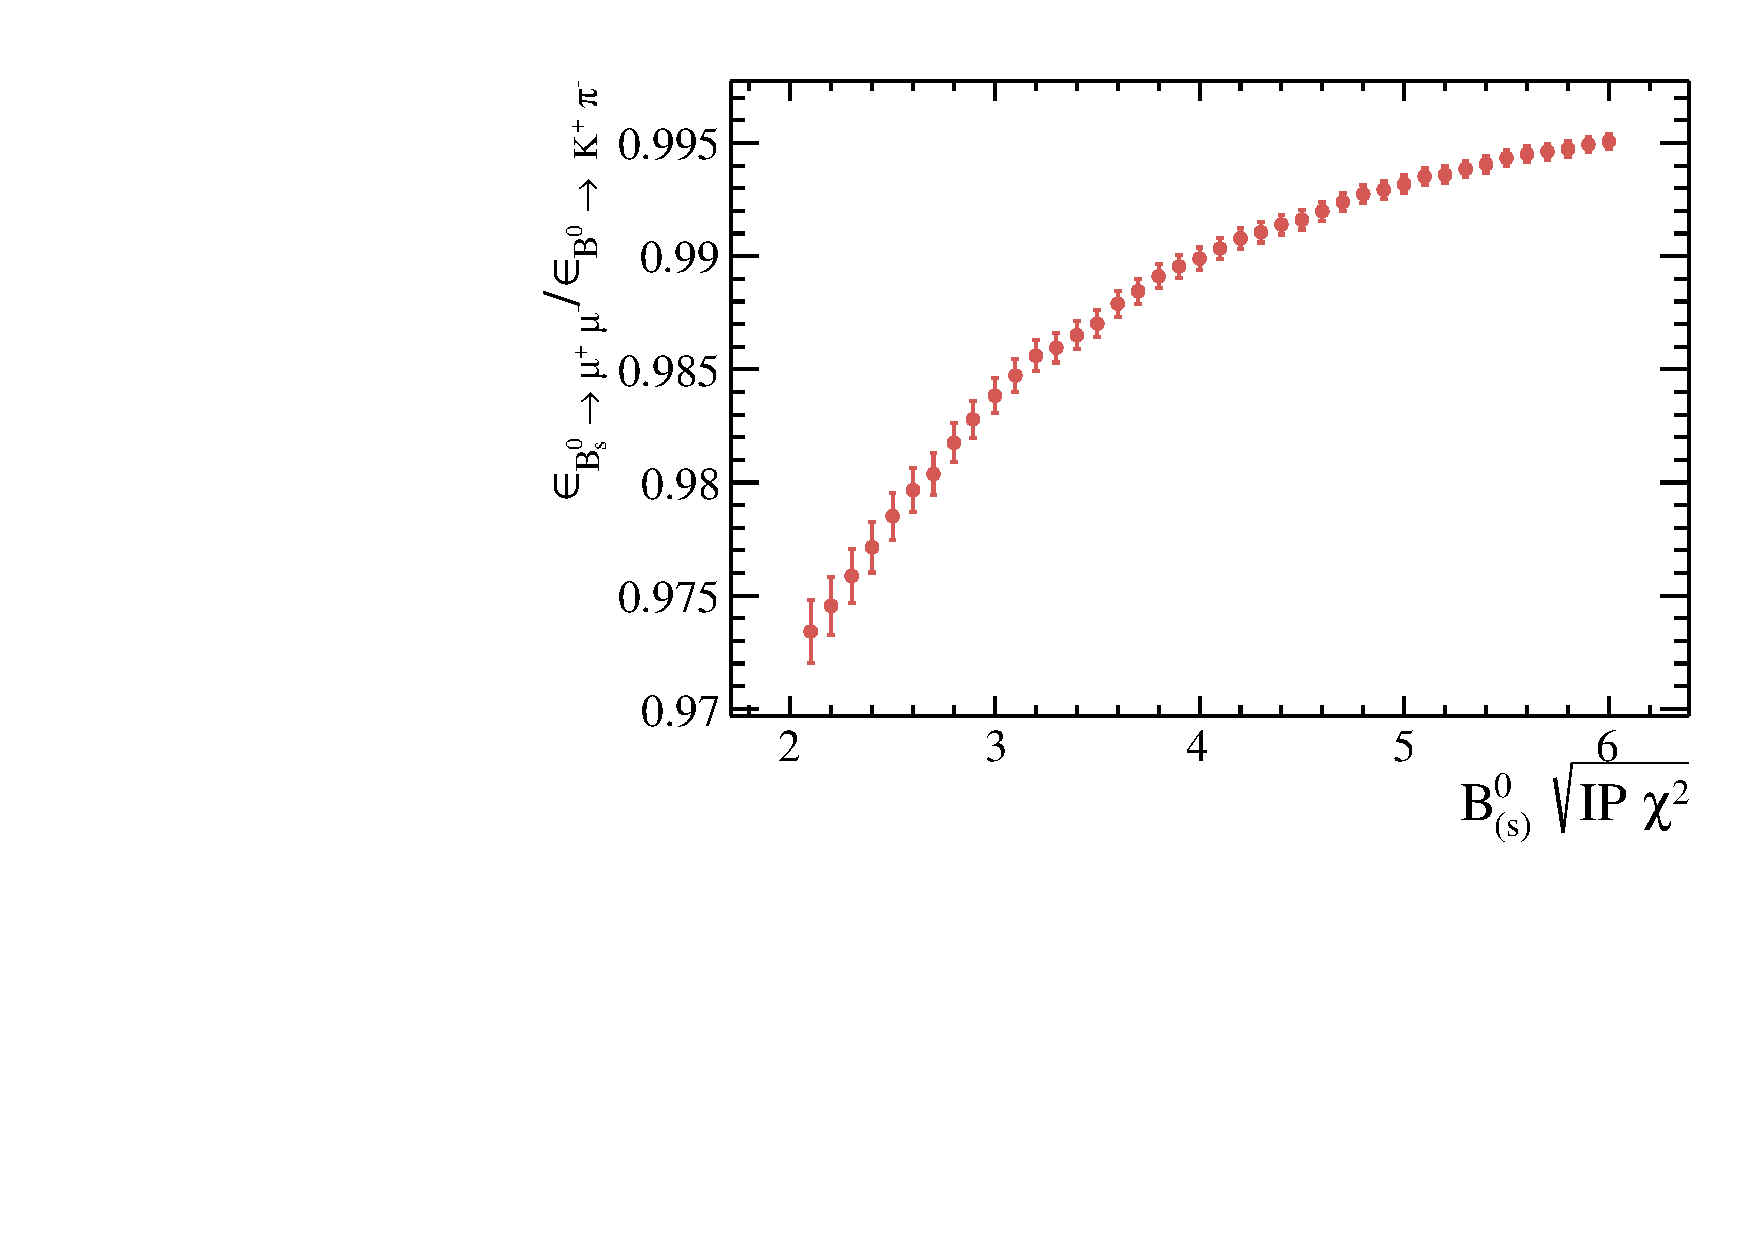
\includegraphics[width=\textwidth]{./Figs/Selection/Bs2MuMu_KPi_IP.pdf}
        %\caption{ }
        %\label{fig:IPS_ratioKPi}
    \end{subfigure}
    ~ %add desired spacing between images, e. g. ~, \quad, \qquad, \hfill etc.                                                                                    
      %(or a blank line to force the subfigure onto a new line)                                                                                                   
    \begin{subfigure}[b]{0.4\textwidth}
        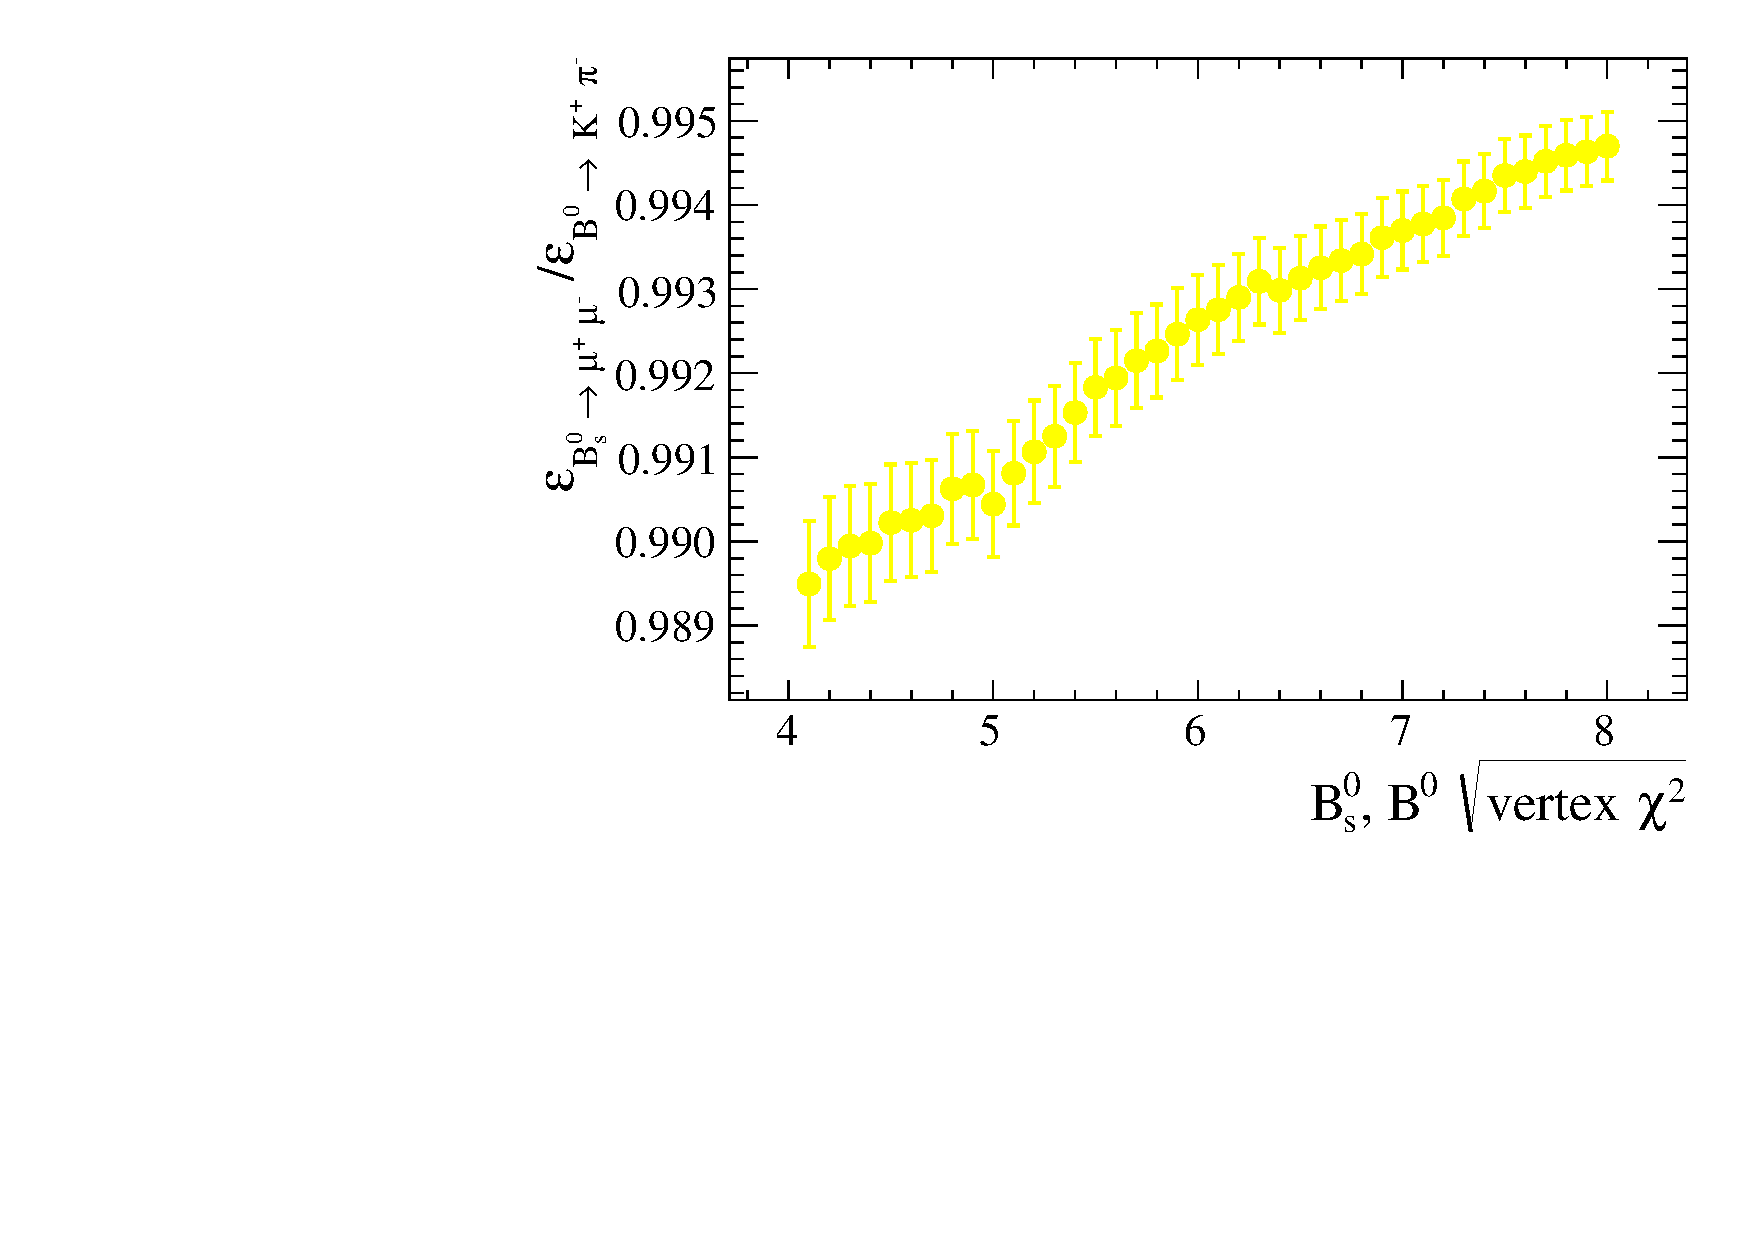
\includegraphics[width=\textwidth]{./Figs/Selection/BSMuMu_KPi_vertex.pdf}
        %\caption{ }
        %\label{fig:CHI2_ratioKPi}
    \end{subfigure}
    ~ %add desired spacing between images, e. g. ~, \quad, \qquad, \hfill etc.                                                                                    
    %(or a blank line to force the subfigure onto a new line)                                                                                                     

    \begin{subfigure}[b]{0.4\textwidth}
        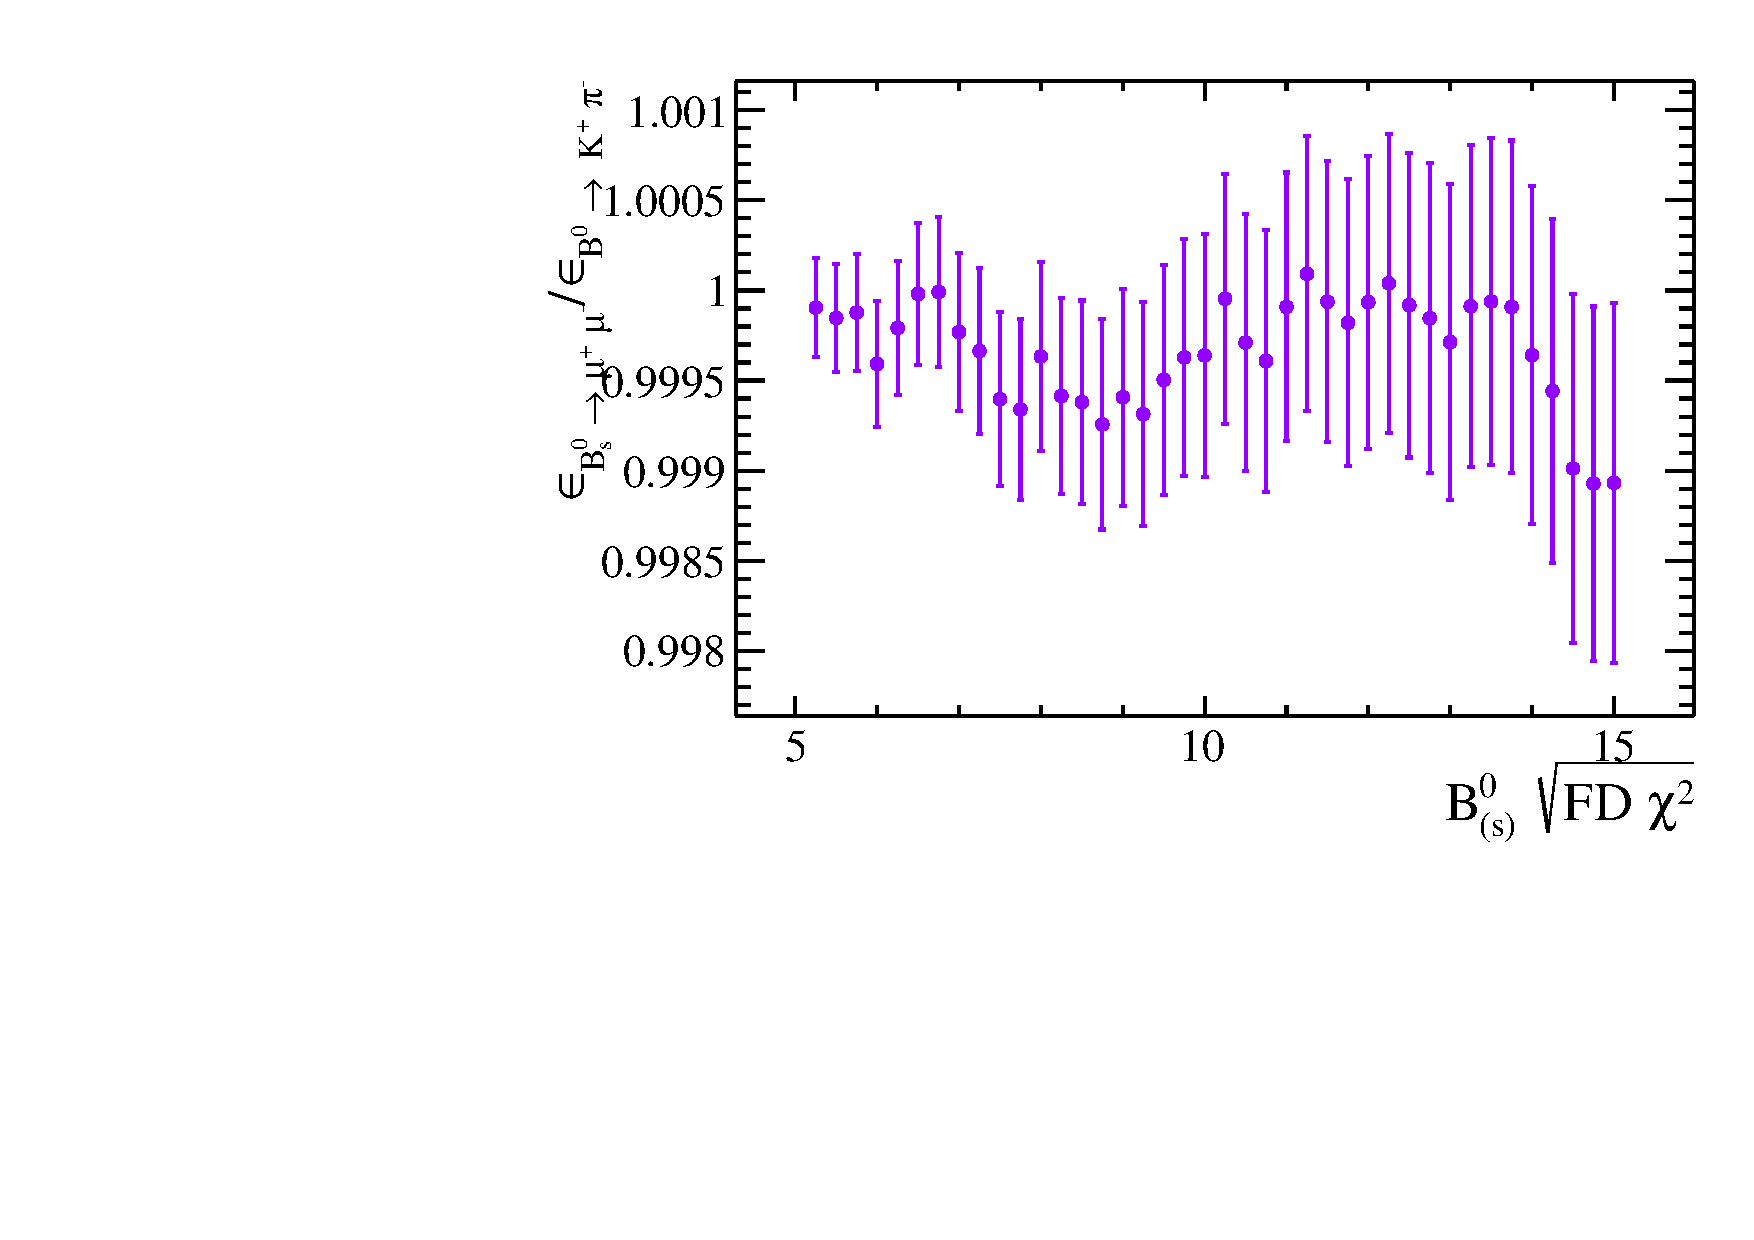
\includegraphics[width=\textwidth]{./Figs/Selection/Bs2MuMu_KPi_FD.pdf}
        %\caption{ }
        %\label{fig:FD_ratioKPi}
    \end{subfigure}
   \begin{subfigure}[b]{0.4\textwidth}
        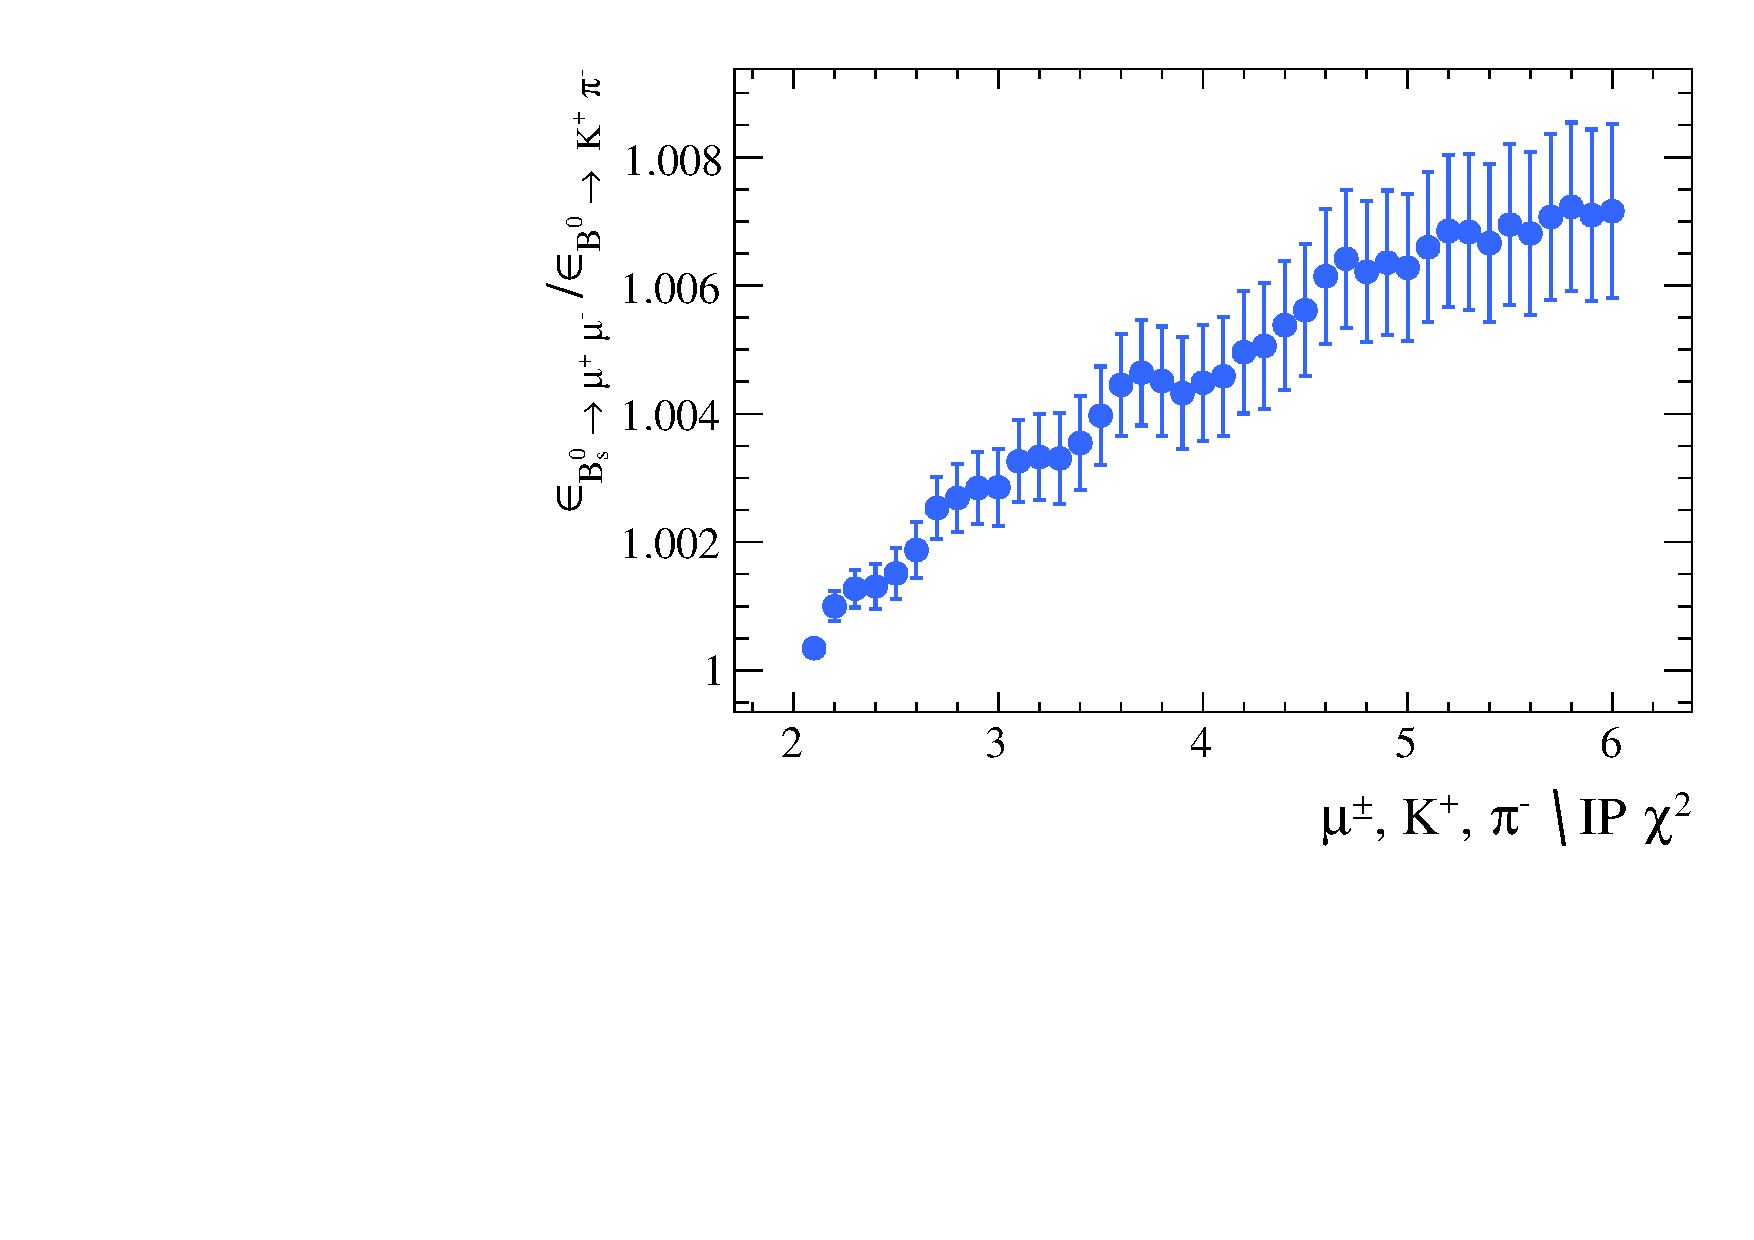
\includegraphics[width=\textwidth]{./Figs/Selection/Bs2MuMu_KPi_daughter_IP.pdf}
        %\caption{ }
        %\label{fig:IPS_ratioKPi}
    \end{subfigure}
    \caption{The ratio of \bsmumu to \bdkpi stripping efficiencies when each cut has been applied independently of all other cuts. The current cut values are marked by the blue lines.}
    \label{fig:ratio_plotsBd2KPi}
\end{figure}


\begin{figure}[htbp]
    \centering
    \begin{subfigure}[b]{0.4\textwidth}
        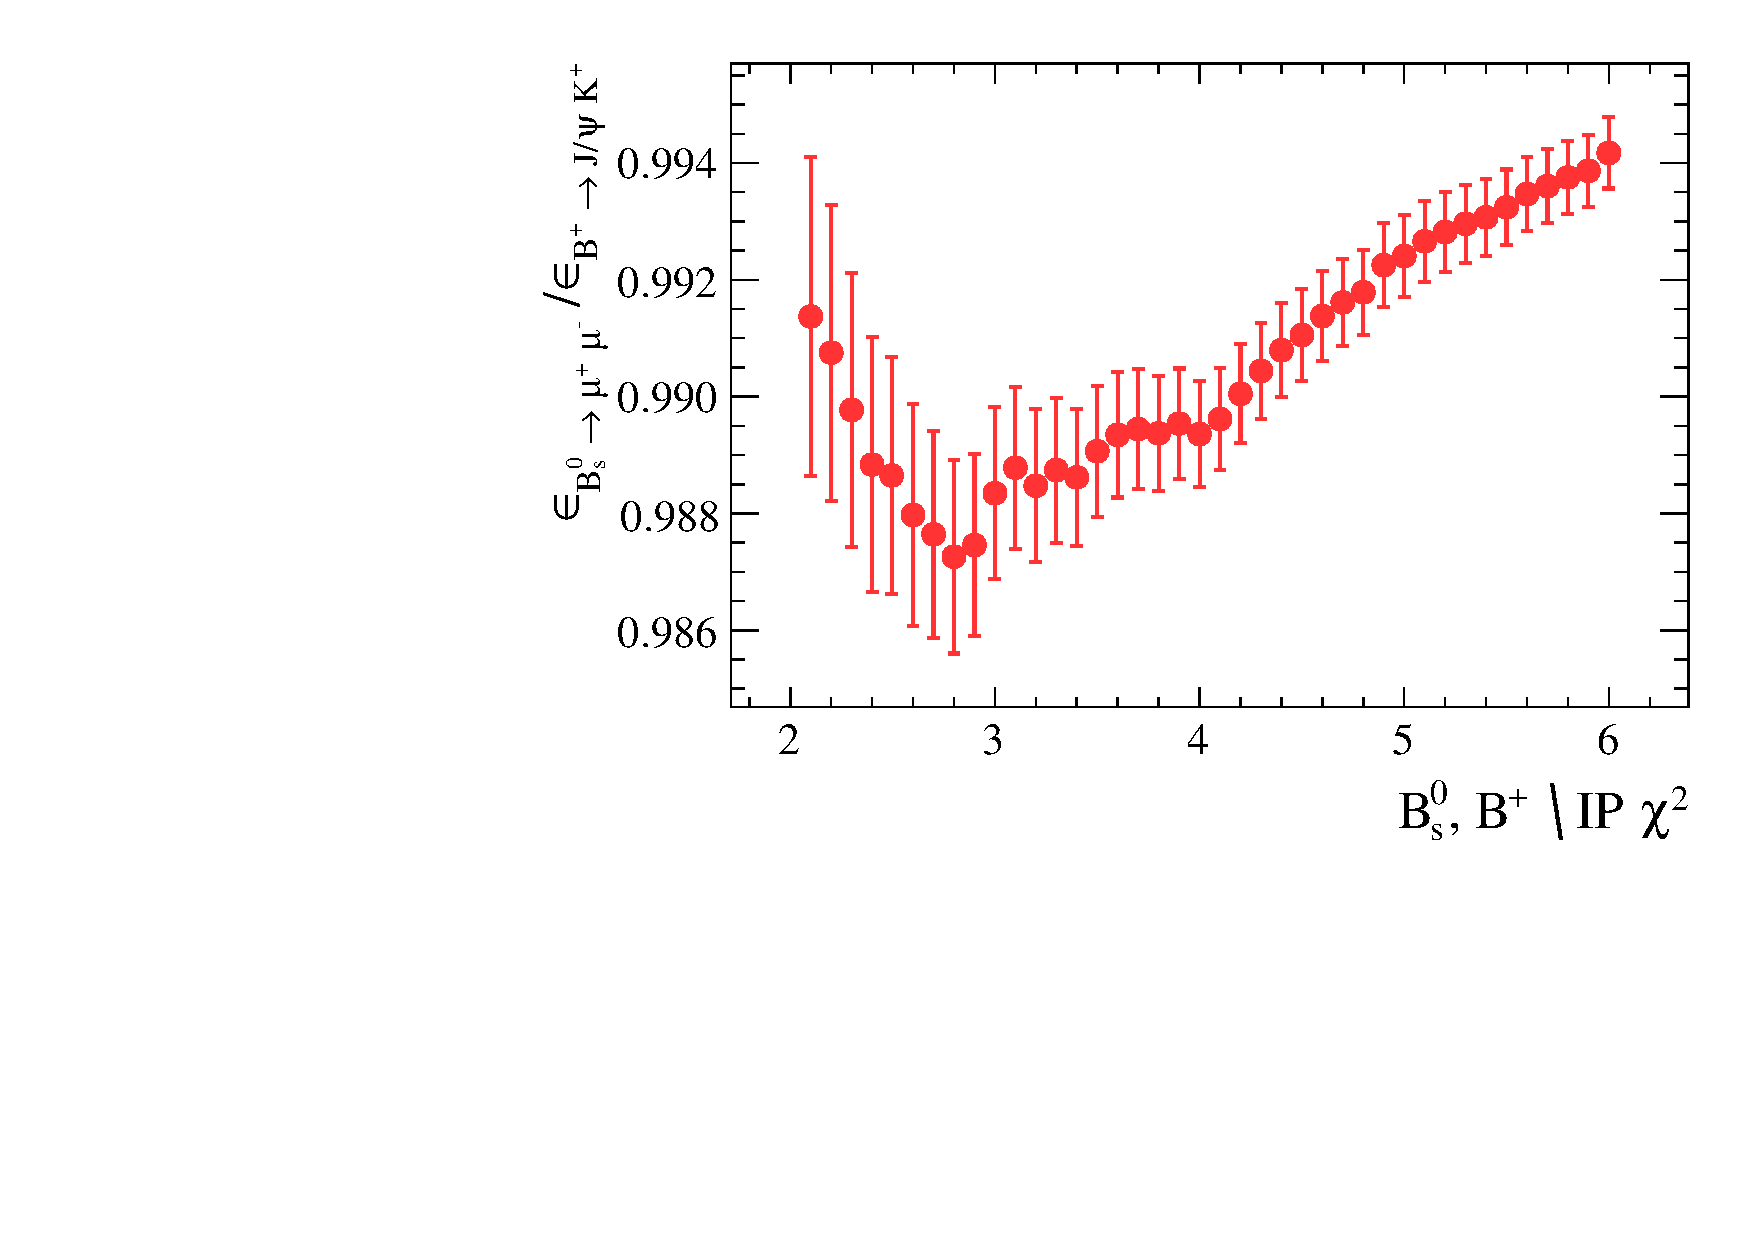
\includegraphics[width=\textwidth]{./Figs/Selection/BsMuMu_JPsiK_IP.pdf}
        %\caption{ }
        %\label{fig:IPS_ratio}
    \end{subfigure}
    ~ %add desired spacing between images, e. g. ~, \quad, \qquad, \hfill etc. 
      %(or a blank line to force the subfigure onto a new line)
    \begin{subfigure}[b]{0.4\textwidth}
        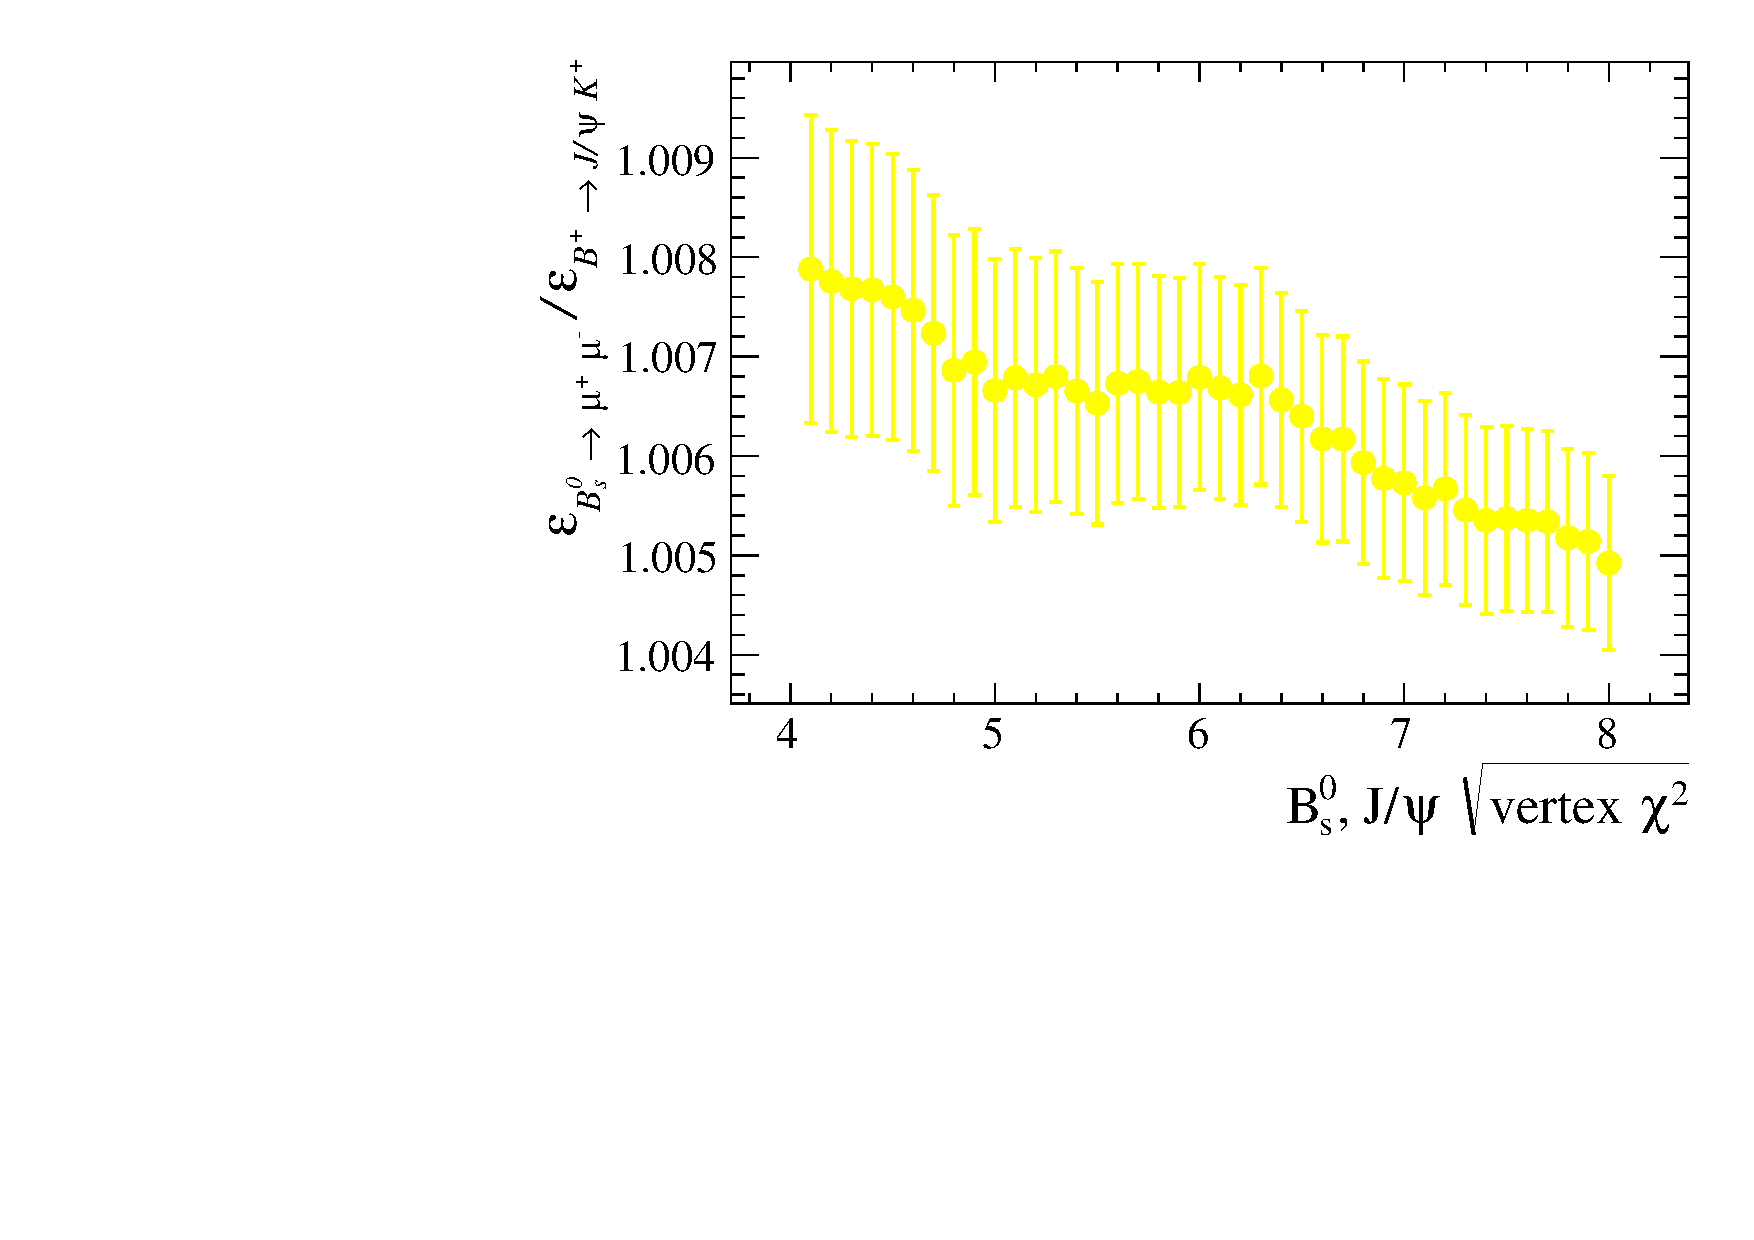
\includegraphics[width=\textwidth]{./Figs/Selection/BsMuMu_JpsiK_vertex.pdf}
        %\caption{ }
        %\label{fig:CHI2_ratio}
    \end{subfigure}
    ~ %add desired spacing between images, e. g. ~, \quad, \qquad, \hfill etc. 
    %(or a blank line to force the subfigure onto a new line)

    \begin{subfigure}[b]{0.4\textwidth}
        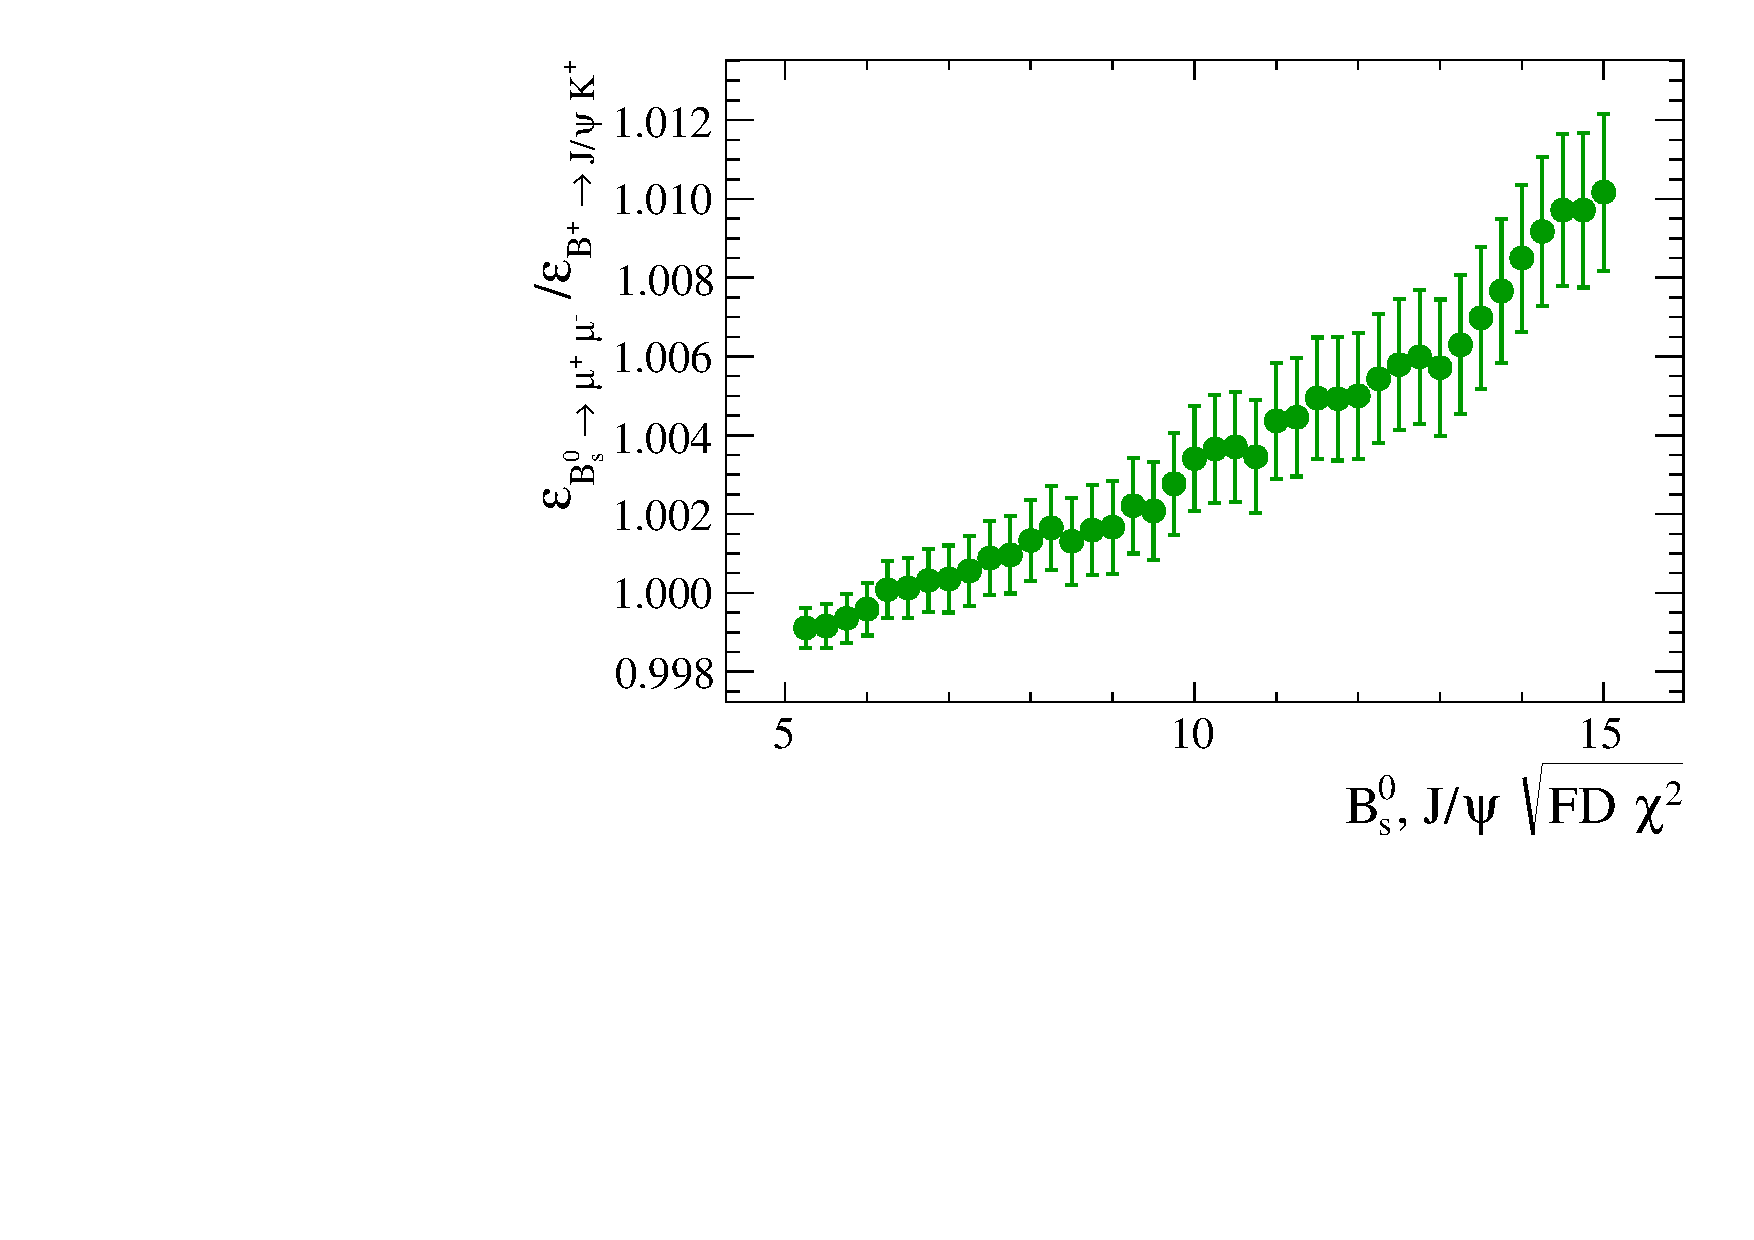
\includegraphics[width=\textwidth]{./Figs/Selection/BsMuMu_JpsiK_FD.pdf}
        %\caption{ }
        %\label{fig:FD_ratio}
    \end{subfigure}
   \begin{subfigure}[b]{0.4\textwidth}
        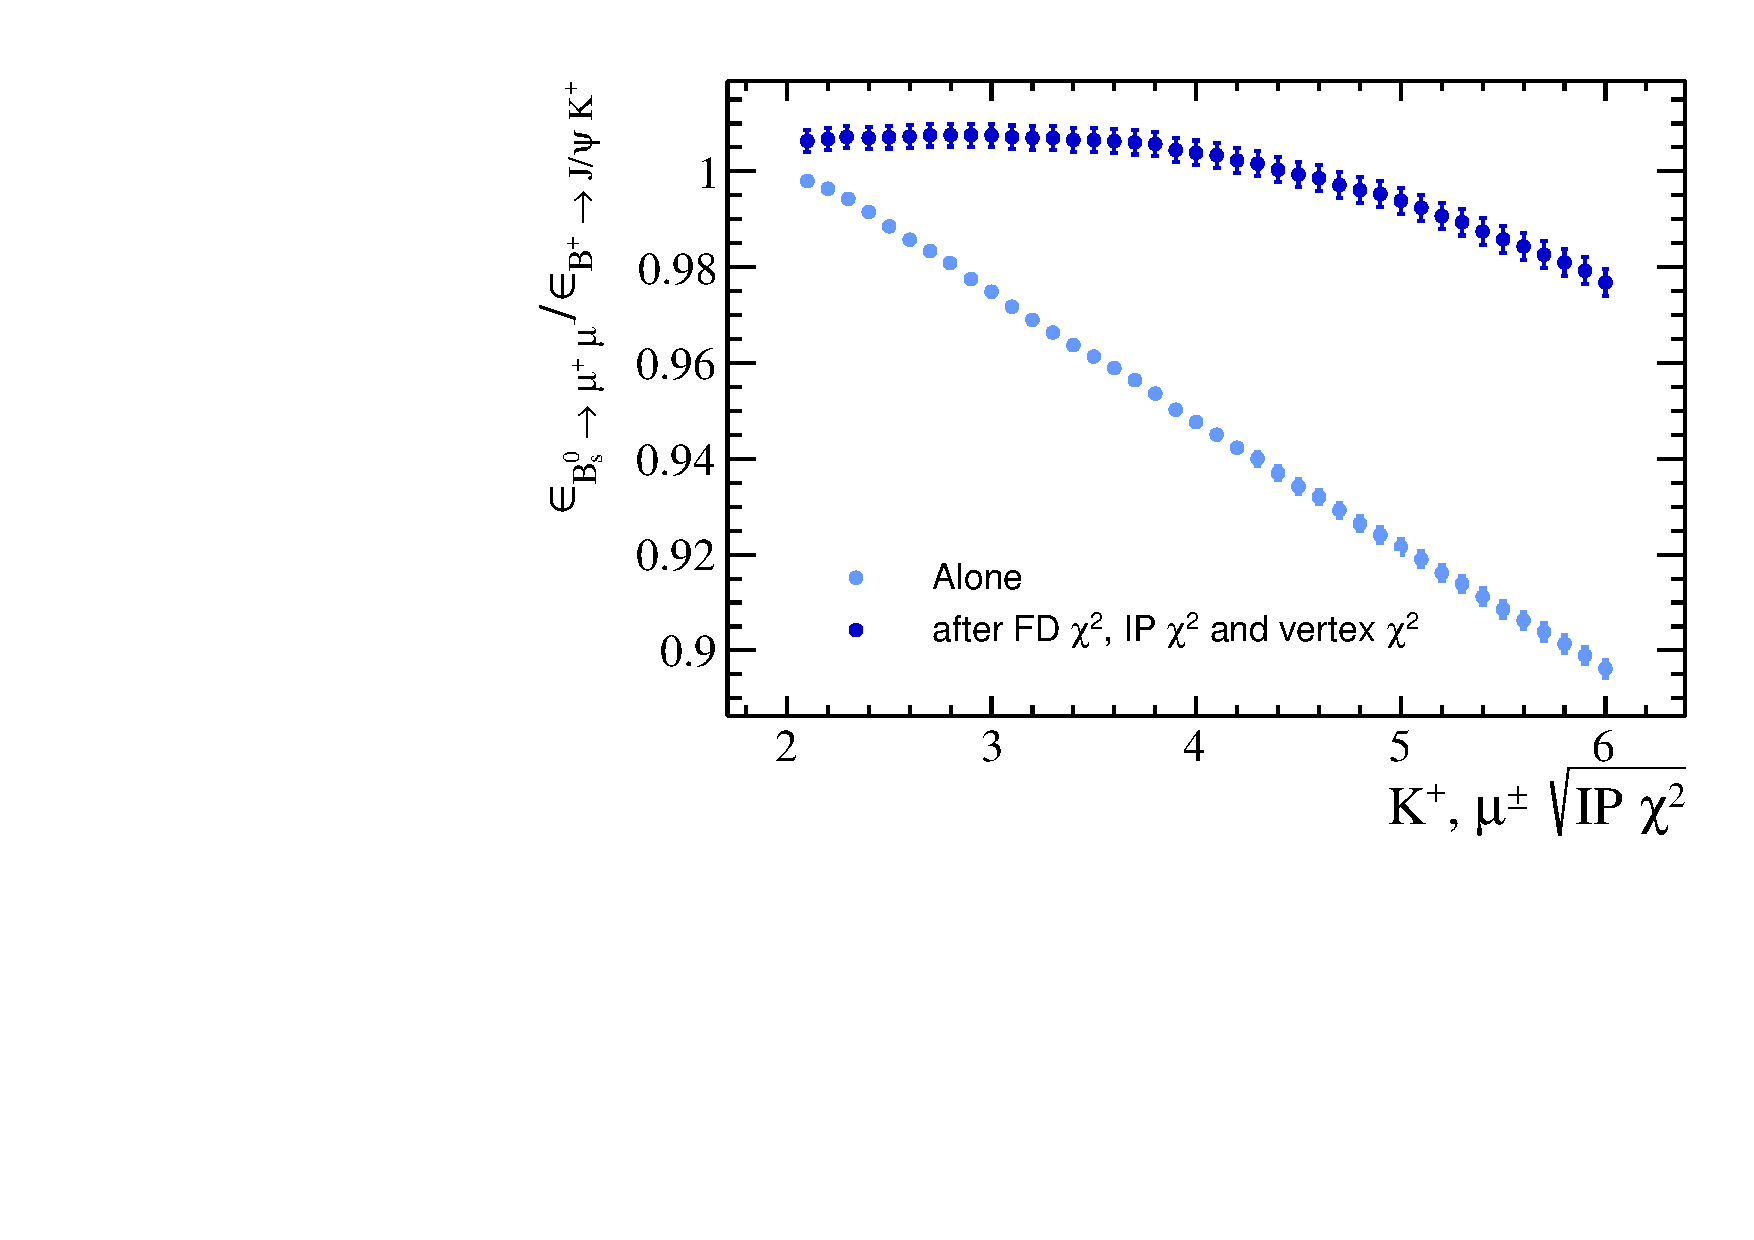
\includegraphics[width=\textwidth]{./Figs/Selection/Bs2MuMu_JpsiK_daughter_IP.pdf}
        %\caption{ }
        %\label{fig:IPS_ratio}
    \end{subfigure}
    \caption{The ratio of $B^{0}_{(s)}\to\mu^{+} \mu^{-}$ to $B^{+}\to J/\psi K^{+}$ stripping efficiencies when each cut has been applied independently of all other cuts. The current cut values are marked by the blue lines.}
    \label{fig:ratioplotsJpsik}
\end{figure}


The efficiencies for most of the stripping cuts as $\sim 97 \%$ or higher, however, the efficiencies of the cuts on the FD $\chi^{2}$ of the \bsd or \jpsi and the daughter IP $\chi^{2}$ of the muon or hadron pair are lower at $83 \%$ and $80 \%$, respectively. Therefore improvements to the stripping selection efficiencies could be achieved by altering these two selection requirements. 



The set of events removed by each cut in the stripping selection is not independent. Therefore the effect of changing one cut on the total efficiency of a stripping selection must be considered. Figure~\ref{fig:efficiencyplots} shows the total efficiency of the \bsmumu stripping line on simulated \bsmumu decays for a range of FD $\chi^{2}$ and daughter IP $\chi^{2}$ cut values. As expected the lower the cut values the more efficient the stripping line becomes. It is important that any increase in \bsmumu selection efficiency from the stripping is not removed when the trigger requirements are applied, Figure~\ref{fig:triggereffplots} shows that the trigger efficiencies are relatively flat across a large range of FD $\chi^{2}$ and daughter IP $\chi^{2}$ cut values therefore the efficiency gained by a change in the stripping selection is not lost when trigger requirements are imposed. The selection efficiency for \bdmumu is very similar to \bsmumu as seen in Table~\ref{tab:Run1strippingEff}, therefore only \bsmumu have been studied for different stripping selection cut values. 


\begin{figure}[htbp]
    \centering
    %\begin{subfigure}[b]{0.4\textwidth}
        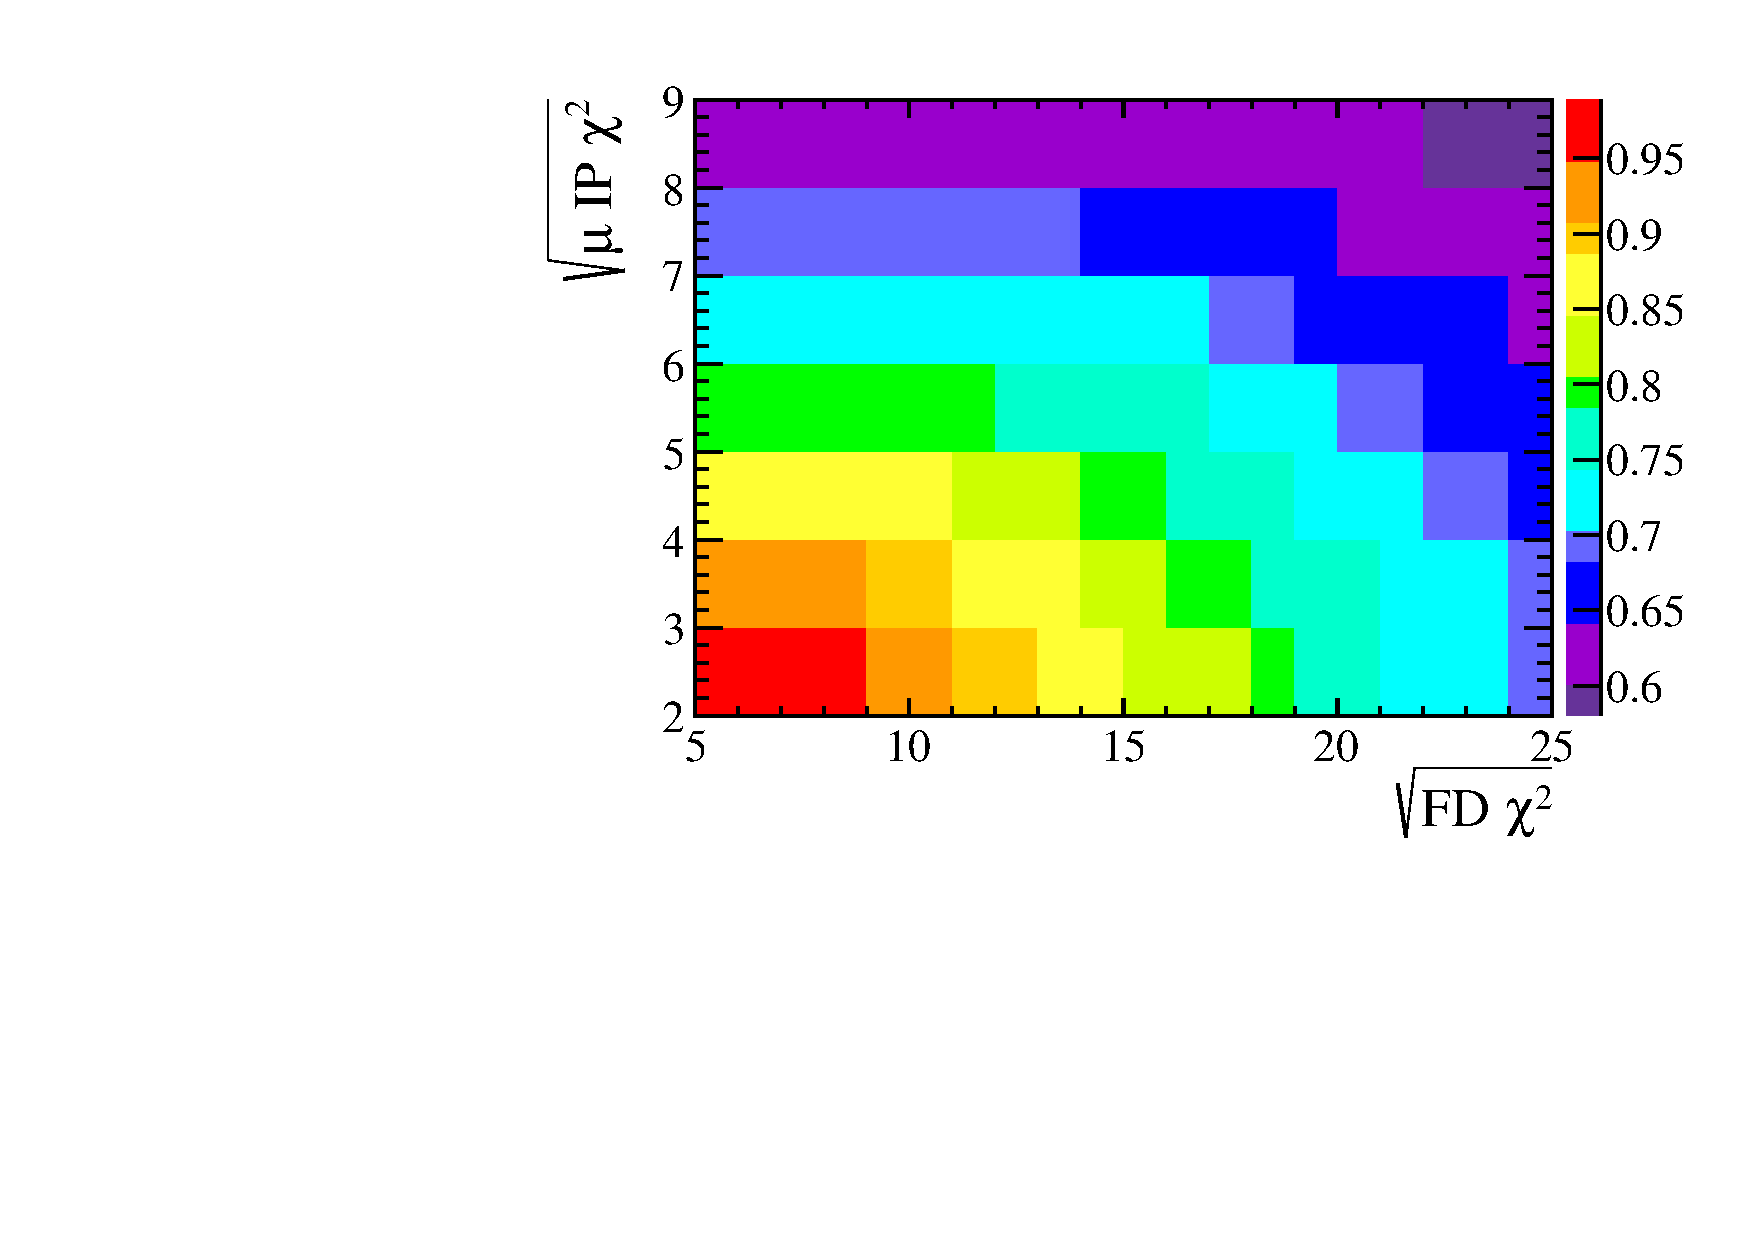
\includegraphics[width= 0.8 \textwidth]{./Figs/Selection/Bs2MuMu_efficiency_chart_Feb3.pdf}
       % \caption{ }
      %  \label{fig:eff}
  %  \end{subfigure}
    ~ %add desired spacing between images, e. g. ~, \quad, \qquad, \hfill etc. 
      %(or a blank line to force the subfigure onto a new line)
   % \begin{subfigure}[b]{0.4\textwidth}
       % \includegraphics[width=\textwidth]{./Figs/Selection/strip_chart1.png}
      %  \caption{ }
      %  \label{fig:eff_contours}
  %  \end{subfigure}
    \caption{Efficiency of the \bmumu stripping selection for \bsmumu simulated decays for a range of cuts on the \bs FD \chisqd and the minimum muon IP \chisqd.}
    \label{fig:efficiencyplots}
\end{figure}

\begin{figure}[htbp]
    \centering
    \begin{subfigure}[b]{0.7\textwidth}
        \includegraphics[width=\textwidth]{./Figs/Selection/TIS_TOS_Trigger_chart.pdf}
        \caption{ }
        \label{fig:TISTOS}
    \end{subfigure}
    ~ %add desired spacing between images, e. g. ~, \quad, \qquad, \hfill etc. 
      %(or a blank line to force the subfigure onto a new line)
    \begin{subfigure}[b]{0.7\textwidth}
        \includegraphics[width=\textwidth]{./Figs/Selection/Dec_trigger_chart.pdf}
        \caption{ }
        \label{fog:Dec}
    \end{subfigure}
    \caption{The trigger efficiencies of \bsmumu simulated decays across a range of \bs FD \chisqd and the minimum muon IP \chisqd cut values. a) shows the efficiencies of the trigger requirements used to select \bsmumu decays for the effective lifetime measurement listed in Table~\ref{tab:triggers} and b) shows the efficiencies of the trigger requirements used to select \bmumu decays for the branching fraction measurement the same trigger lines in Tables~\ref{tab:triggers} are used but candidates must pass the DEC trigger decision at each level. }
    \label{fig:triggereffplots}
\end{figure}





One of the main purposes of the stripping selection, as described in Section~\ref{SoftwareSimulation}, is to reduce the size of the data set, therefore the cuts cannot be set as loose as possible. 

Any change applied to the \bmumu stripping line must be propagated through into the stripping lines for \bhh and \bujpsik decays therefore the retention of all stripping lines must be evaluated.

Table 3.5 %~\ref{tab:Retention} 
shows the total efficiency of the \bsmumu stripping line along side the amount of data retained for the set of cuts on the FD \chisqd and daughter IP \chisqd for the \bmumu, \bhh and \bujpsik stripping lines. The set of chosen cuts aims to keep both cuts as high as possible for a certain \bsmumu efficiency. 



\afterpage{
\begin{landscape}
\vspace*{\fill}
\begin{table}[htbp]
\begin{center}
\begin{tabular}{ cc|c|ccc}\hline
                       	\multicolumn{2}{c}{Stripping cut}                   & Stripping line efficiency &  \multicolumn{3}{c}{Stripping line retention} \\
\hline
$\sqrt{\text{FD} \chisqd}$ & Daughter  $\sqrt{\text{IP} \chisqd}$ & \bsmumu  	& \bmumu 	& \bdkpi & \bujpsik \\
\hline
15                    		&5.00                 			& (71.29 $\pm$ 0.07) $\%$  	&  1.0      	&1.0     &1.0        \\
14                  	  	&4.25                  		& (74.91 $\pm$ 0.07) $\%$  	&  1.5      	&1.3     &1.1        \\
13                    		&4.00                  		& (76.84 $\pm$ 0.07) $\%$  	&  1.8      	&1.5     &1.2        \\
12                    		&3.50                  		& (79.76 $\pm$ 0.07) $\%$  	&  2.6      	&1.8     &1.3        \\
11                    		&3.00                  		& (82.72 $\pm$ 0.06) $\%$  	&  3.7      	&2.4     &1.6        \\
10                    		&2.75                  		& (84.86 $\pm$ 0.06) $\%$  	&  4.7      	&3.0     &1.7        \\
9                     		&2.50                  		& (86.96 $\pm$ 0.06) $\%$  	&  6.8      	&3.9     &2.0        \\
\hline
\end{tabular}
\end{center}
\label{tab:Retention}
\vspace{0.7cm}
\caption{The efficiency of the \bmumu stripping line to select \bsmumu decays and the changing in the date retention for \bmumu, \bhh and \bujpsik stripping lines for a range of FD \chisqd and daughter IP \chisqd cut values. Fractional uncertainty on the retention is less than 1 $\%$.}
\end{table}
\vspace*{\fill}
\end{landscape}
}







The data retention is computed by applying the stripping selection to a sub-set of 2012 data to find the number of events that pass the stripping lines for each pair of FD $\chi^{2}$ and daughter IP $\chi^{2}$ cuts. No trigger requirements are imposed on trigger lines because the stripping selection run on the full output of the trigger. The number of events for each set of cuts is normalised to the number of events passing the original Run~1 stripping line requirements  to show the fractional increase caused by loosening the cut values. 

An increase of 15~$\%$ can be gained in the stripping selection efficiencies by using the loosest cuts in Table 3.5 %\ref{tab:Retention} 
however the loosest cuts increases the amount of data passing the \bmumu stripping selection by a factor of 7 and the \bhh stripping selection by a factor of 4. Table~\ref{tab:NumEvents} shows the number of Run~1 candidates passing the original stripping selection listed in Table~\ref{tab:PreviousStripping} for the last published analysis. The \bhh stripping line lets through the most candidates where as the \bmumu stripping line saves far fewer candidates, therefore a chance in the retention of the \bhh line is more significant than the \bmumu line. 


The final set of cuts used in the stripping selection must be a compromise between the selection efficiency and the amount of data that passes the selection. The selection cuts of \bs FD $\chi^{2}$ $>$ 121 and minimum muon IP $\chi^{2}$ $>$ 9 would increase the \bmumu selection efficiency by from 71~$\%$ to 82~$\%$ and the amount of data retained would be doubled. The increase of the data retained by the \bhh and \bujpsik lines is smaller and the efficiencies are similar to the \bmumu selection efficiencies. Therefore these cuts are applied in the stripping selection for this analysis. %However the increase in efficiency after the stripping selection will not necessarily be propagated through the whole analysis. 



\begin{table}[htbp]
\begin{center}
\begin{tabular}{lcc}
\hline
Stripping Lines & Events & Retention / $\%$ \\
\hline
\bmumu & 898880 & 0.0022 \\
\bhh & 14502295  &  0.0831 \\
\bujpsik & 3344568 & 0.0087  \\
%\bjpsiphi & 456787  & 0.0011 \\
%$B \to J/\psi K^{*}$ &  12574956 & 0.018 \\
\hline
%Total & 31779975& - \\
%Total with correlation & 31402536 \\
Total & 18745743& - \\
\hline
\end{tabular}
\vspace{0.7cm}
\caption{The number of events passing stripping lines used for the \bsmumu analysis from the selection listed in Table~\ref{tab:PreviousStripping} and the percentage of the total LHCb data set that they correspond to. The total does not include correlation between lines, which is expected to be 42 $\%$ between \bmumu and \bhh lines. }
\label{tab:NumEvents}
\end{center}
\end{table}





\subsection{Stripping selection and offline cuts}
\label{finalloosesel}


The complete list of selection cuts applied in the cut based selection to select \bsmumu and \bhh decays in Run~1 and Run~2 data are listed in Tables~\ref{tab:fullpreselection}. The stripping selection cuts from Table~\ref{tab:PreviousStripping} are included with the $B$ mesons FD \chisqd and daughter IP \chisqd requirements updated to the looser values and the selection of \bmumu decays includes the momentum, ghost track probability and decay time cuts made in the \bhh stripping line, but were absent in the \bmumu stripping line.

Additional selection requirements are applied after the stripping to remove specific backgrounds. A lower bound is placed on the $B$ meson transverse momentum to remove pairs of muons originating from $pp \to p\mu^{+}\mu^{-} p$ decays and a \jpsi veto is used to remove backgrounds from \bcjpsimunu decays. The semi-leptonic \bcjpsimunu decays, where \jpsimumu, contribute to the background of \bmumu decays when a muon from the \jpsi forms a good vertex with the muon from the $B_{c}^{+}$ decay. Due to the high mass of the $B_{c}^{+}$ this could place mis-reconstructed candidates within the \bs mass window. A `\jpsi veto' can be used to remove background events from \bcjpsimunu decays. The veto works by removing events where one muon from the \bmumu candidate combined with any other oppositely charged muon in the event has $m_{\mu^{+}\mu^{-}}$ -$ m_{J/\psi}} < 30$  \mevcc. %The veto has a rejection power of X  $\%$ on \bcjpsimunu events that have passed \bmumu other selection cuts in Table~\ref{tab:fullpreselection} and rejects only  $\%$ of \bmumu signal events. The expected number of \bcjpsimunu events after the full selection can be found in Section~X. 

The $B$ meson mass range for both \bsmumu and \bhh decays is narrower than the range in the stripping selection in Section~\ref{strippingold}. \bsmumu candidates are required to have a dimuon invariant mass greater than 5320 \mevcc. The motivation comes from mass fit studies that are detailed in Section X. The consequence of this cut is to remove \bdmumu decays, $B_{s}^{0} \to \mu^{+} \mu^{-} \gamma$ backgrounds and most backgrounds from mis-identified semi-leptonic and \bhh decays. This can be seen from the mass distribution in Figure~\ref{fig:LHCbCMS}. The expect number of \bdmumu and mis-identified decays after the full selection can be found in Section~X. Similarly the \bhh mass window is reduced to remove contributions from mis-identified backgrounds. 

The selection applied to Run~1 and Run~2 is the same for all variables expect the track ghost probability and track \chisqd/$ndof$. Slightly looser cuts are used for Run~2 to take advantage to changes in the reconstruction that were introduced for Run~2. 

%\begin{landscape}
%\vspace*{\fill}
\begin{table}[htbp]
\begin{center}
\begin{tabular}{lll}
\hline
Particle                & \bsmumu                                     & \bhh                                 \\
\hline
\bs or $B^{+}$          & 5320 \mevcc $<$ M $<$ 6000 \mevcc           & 5100 \mevcc $<$ M $<$ 5500  \mevcc      \\                          
                        & DIRA $>$ 0                                    & DIRA $>$ 0                             \\
                        & FD $\chi^{2}$ $>$ 121                       & FD $\chi^{2}$ $>$ 121                  \\       
                        & IP $\chi^{2}$ $<$ 25                        & IP $\chi^{2}$ $<$ 25                   \\
                        & Vertex $\chi^{2}$/ndof $<$ 9                  & Vertex $\chi^{2}$/ndof $<$ 9              \\      
                        & DOCA $<$ 0.3 mm                             & DOCA $<$ 0.3 mm                          \\    
                        & $\tau$ $<$ 13.248 \ps                       & $\tau$ $<$ 13.248 \ps                \\
                        & $p_{T}$ $>$ 500 \mevc                        & $p_{T}$ $>$ 500 \mevc                \\

\hline
Daughter $\mu$ or $h$   & Track $\chi^{2}$/ndof $<$ 3 (4)               & Track $\chi^{2}$/ndof $<$ 3 (4)         \\                       
                        & Minimum IP $\chi^{2}$ $>$ 9                 & Minimum IP $\chi^{2}$ $>$ 9           \\             
                        & 0.25 \gevc $<$ $p_{T}$ $<$ 40 \gevc         & 0.25 \gevc $<$ $p_{T}$ $<$ 40 \gevc    \\
                        & $p$ $<$ 500 \gevc                             & $p$ $<$ 500 \gevc                       \\
                        & ghost probability $<$ 0.3 (0.4)             & ghost probability $<$ 0.3 (0.4)   \\
                        & $|$m_{\mu\mu} - m_{\jpsi}$| $<$ 30$~\mevcc        &$|$m_{\mu\mu} - m_{\jpsi}$| $<$ 30$~\mevcc    \\
                        & isMuon = True                               &  -                                \\

\hline

\hline
\end{tabular}
\vspace{0.7cm}
\caption{Selection cuts applied to select \bsmumu and \bhh decays, where selection is different between Run~1 and Run~2 the Run~2 values are shown in parenthesis.}
\label{tab:fullpreselection}
\end{center}
\end{table}
%\vspace*{\fill}
%\end{landscape}



\section{Particle Identification}
\label{sec:PID}
Particle identification (PID) variables are used to refine the selection of \bsmumu candidates and to separate different \bhh decays. 

In the selection of \bsmumu decays PID variables are particularly useful to reduce the backgrounds coming from mis-identified semi-leptonic decays and \bhh decays and also help to reduce the number of combinatorial background events. However most backgrounds from mis-identified semi-leptonic and \bhh decays are below the mass cut applied to \bsmumu candidates at 5320~\mevcc therefore loose PID requirements can be used to select \bsmumu decays ensuring a higher signal selection efficiency.

The PID requirements to select \bmumu decays are shown Table~\ref{} alongside requirements to separate different \bhh decays. Two types of PID variables, defined in Section~\ref{PID_variables}, are used; DLL variables and ProbNN variables. 

%A linear combination of ProbNN variables is used to select \bsmumu decays and remove semi-leptonic backgrounds. 
A linear combination of ProbNN variables is used to select \bsmumu decays and remove semi-leptonic backgrounds, in addition to the isMuon requirement applied in the stripping selection.
The classifiers used in ProbNN variables are tuned to give the best performance depending on the different data taking conditions in the detector for each year. %The efficiency of a cut on the linear combination of ProbNN variables to select \bsmumu decays and to reject background decays depends on the ProbNN tune being used. 
Since different tunes are used to select \bsmumu decays in 2016 data compared to Run~1 and 2015 data, the requirement on the linear combination of ProbNN variables varies with the year of data taking. The cuts are chosen to give similar efficiencies for each data sets at selecting signal and removing background across the different years. 



The separation of different \bdkpi and \bskk decays is done via DLL variables. These are useful to separate \bhh decays where $h$ is either a pion or kaon because the variables compare different particle hypotheses with the pion hypotheses. The selection requirements used are the same for each year of data taking.

\afterpage{
\begin{landscape}
\vspace*{\fill}
\begin{table}[htbp]
\begin{center}
\begin{tabular}{lll}
\hline
Decay                    & Particle               & PID requirements \\
\hline
\bsmumu  (Run~1 and 2015) & $mu^{+}$ and $\mu^{-}$ & ProbNN$\mu$ * (1 - ProbNN$\pi$) * (1 - ProbNN$p$) > 0.2 \\
\bsmumu  (2016)          & $mu^{+}$ and $\mu^{-}$ & ProbNN$\mu$ * (1 - ProbNN$\pi$) * (1 - ProbNN$p$) > 0.4 \\
\bdkpi and \bskpi       & $K^{+}$                & DLL$_{K\pi}$ $>$ 10 \\
                         & $\pi{-}$              & DLL$_{K\pi}$ $<$ -10 \\
\bskk                    & $K^{+}$ and $K^{-}$    & DLL$_{K\pi}$ $>$ 10 \\
\hline
\end{tabular}
\vspace{0.7cm}
\caption{Particle identification requirements to select \bsmumu decays and to separate the \bhh decays \bdkpi and \bskpi from \bskk. }
\label{tab:PID}
\end{center}
\end{table}
\vspace*{\fill}
\end{landscape}
}



\section{Multivariate Classifiers}
\label{sec:MVC}

The selection described so far remove a large number of background candidates however because \bsmumu decays occur very rarely the data is still dominated by long lived combinatorial background from \bbbarmumux decays. To increase the signal purity of the data multivariate classifiers are used to separate \bsmumu from the backgrounds.

A multivariate classifier is an algorithm that learns differences between signal and background decays. The classifier is given two input samples, one contain only signal decays and the other containing just background decays and a set of input variables. These input variables have different distributions for signal and background decays. The classifier uses the distributions of the input variables along with its knowledge of which decays are signal and background to learn the difference between the two types. The algorithm can then be applied to a data set containing an unknown mixture of signal and background decays to separate them. For each decay the algorithm produces a number, typically between -1 and +1, where high numbers indicate signal-like decays and low numbers indicating background-like decays. A cut is placed on the output of the classifier to remove background so that the remaining data set has a higher purity for signal events.

Two multivariate classifiers are used to select \bsmumu decays. Both classifiers are a type called a Boosted Decision Tree (BDT) that are described in Section~\ref{sec:GeneralBDT}. A range of different classifiers were investigated but BDTs preformed the best at separating signal from background. 

The first classifier (Sect.~\ref{BDTS}), called the BDTS, is used to remove candidates that are very unlikely to be signal and has a high efficiency to select \bsmumu decays. The second classifier (Sect.~\ref{sec:globalBDT}), called the global BDT, is the final step in the selection process, the output is used to remove most of the remaining backgrounds and has much lower efficiency to select signal events compared to the BDTS. The cut applied to the output of this classifier is optimised to give the lowest expected uncertainty on the measurement of the \bsmumu effective lifetime (Sect.~\ref{sec:globalBDToptimisation}).

Both classifiers were developed for the measurement of the \bmumu Branching Fractions. In the selection \bsmumu decays for this analysis the second classifier is used to classify candidates into 8 bins containing increasing proportions of signal candidates, no candidates are removed based on the output of the second BDT. Therefore the BDTS is necessary to reduce the number of background events to a more manageable level. The use of a single classifier was investigated to select candidates to measure the \bsmumu effective lifetime however it was found that the two classifiers developed for the Branching Fraction measurement performed best. 

\subsection{Boosted Decision Trees}
\label{sec:GeneralBDT}
A BDT is made up of the combined outputs of separate decision trees. A decision tree begins with a data sample, where each decay is know to be signal or background and a set of variables describing them. The decision tree applies a cut on a variable that will be the most effective at separating the signal and background in the sample and creates two sub-samples. Another cut is then applied to each of the sub-samples to further separate signal from background. This process is repeated until either a certain number of cuts, defined as the depth of the tree, or the number of candidates in each sub-sample has reached a minimum number. Each sub-sample produced at the end of the tree is called a leaf. The tree uses the knowledge of whether decays are signal or background to assign a value of +1 or -1 to every decay. A decay is given a value +1 if it is in a leaf where the majority is signal and the value -1 if it is in a leaf that has a majority of background decays. The final decisions made by the tree are not prefect, some signal (background) decays will be mis-classified as background and given the value of -1 (+1). %The decision making process of a decision tree is illustrated in Figure~\ref{fig:DT}.

%\begin{figure}
 %   \centering
    %\begin{subfigure}[b]{0.4\textwidth}                                                                                                                          
  %      \includegraphics[width=\textwidth]{./Figs/placeholder.jpeg}
       % \caption{ }                                                                                                                                              
      %  \label{fig:eff}                                                                                                                                          
  %  \end{subfigure}                                                                                                                                              
   % ~ %add desired spacing between images, e. g. ~, \quad, \qquad, \hfill etc.                                                                                    
      %(or a blank line to force the subfigure onto a new line)                                                                                                   
   % \begin{subfigure}[b]{0.4\textwidth}                                                                                                                          
       % \includegraphics[width=\textwidth]{./Figs/Selection/strip_chart1.png}                                                                                    
      %  \caption{ }                                                                                                                                              
      %  \label{fig:eff_contours}                                                                                                                                 
  %  \end{subfigure}                                                                                                                                              
   % \caption{Illustration of a decision tree.}
   % \label{fig:DT}
%\end{figure}

One decision tree on its own is often not particularly good at classifying events, there is no way to correct mis-classified events in the leaves, and it is particularly sensitive to statistical fluctuations in the training samples. A BDT combines the output of numerous decision trees to improve the classification of events and reduce the dependence of the final decisions on statistical fluctuations. A BDT starts with one decision tree and assigns weights to decays in the signal and background samples depending on whether the output of the decision tree classified the events correctly or incorrectly. The weighted sample is then used as the input for the training of the next decision tree. The weights are designed so that the next tree is more likely to correctly classify previously mis-classified events. This process is repeated until a certain number of trees have been trained. The re-weighting process is known as boosting and the weights applied to the samples are taken into account when combining the output of each decision tree into the overall output of the BDT. The output of a BDT will be a number between -1 and +1 where high numbers indicate signal and low numbers indicating background.


The TMVA package~\cite{Hocker:2007ht} is use to develop and train the BDTs, the package provides several different methods of boosting that can be used. The adaptive boosting method was found to produce the most effective BDT.
This method of boosting assigns decays incorrectly classified by one tree the weight, $w$, before being used as the input to the next decision tree. The weights assigned are given by
\begin{equation}
w = \frac{1 - f}{f}\text{, where } f = \frac{\text{total misclassified events}}{\text{total events}}.
\end{equation}
Therefore incorrectly assigned candidates are given a higher weight than correctly classified candidates. The `speed’ at which the boosting occurs is controlled by a the parameter $\beta$ where $w \rightarrow w^{\beta}$, this can be specified in the training of the decision tree and a large number of boosting steps can improve the performance of the BDT.

The ability of a BDT to correctly identify signal and background candidates depends on three main factors;
\begin{itemize}
\item the size of the training samples - a large training sample is useful to prevent the BDT from being sensitive to statistical fluctuations and contains more information the classifier can use to learn the difference between signal and background
\item the input variables - different distributions in the input variables for signal and background candidates enable the classifier to easily separate the types of candidates, the overall performance is insensitive to poorly discriminating variables that are included
\item parameters that dictate the BDT training - the training of a BDT is specified by several parameters; the number of trees (NTrees), the tree depth (MaxDepth), the minimum number of events a leaf can contain (nEventsMin or MinNodeSize\footnote{nEventsMin is the minimum number of decays in a lead where as MinNodeSize is the number of decays in a leaf given as a percentage of the training sample size. The parameter specified in the training depends on the version of the TMVA package used. });, the `speed’ at which the boosting occurs ($\beta$) and the number of cut values that a tree tries for a variable before making a decision (nCuts).
\end{itemize}

These three factors affect the performance of the BDT however the importance of each varies. Together they can be used to prevent the BDT being very sensitive to the statistical fluctuations in the training sample. This  is called overtraining, an overtrained BDT is extremely accurate at classifying the candidates in the training sample by preforms poorly at classifying candidates in a statistically independent sample. Although this is less common in BDT than single decision trees, it can be avoided by having a sufficiently large training sample or by limiting the depth of trees or the number of trees in the BDT. 

\subsection{The BDTS}
\label{BDTS}
%The output of the stripping selection still includes many background decays, further cuts shown in Table~\ref{} reduce the background decays. Some selection cuts are designed to remove specific background decays and the selection for \bsmumu decays used in the Branching Fraction and effective lifetime analyses starts to diverge slightly.

%The BDTS is a multivariate classifier that is designed to reduce the number of combinatorial background events. It is a Boosted Decision Tree (BDT) (see Section~\ref{} for a detailed description) that is trained on \bsmumu and \bbbarmumux simulated decays that have passed the \bmumu selection requirements in Table~\ref{} and additional particle identification cuts listed in Table X. 
The BDTS uses input variables similar to those in the stripping selection to classify events;
\begin{itemize}
\item impact parameter \chisqd of the \bs
\item vertex \chisqd of the \bs
\item direction cosine of \bs
\item distance of closest approach of the muons
\item minimum impact parameter \chisqd of the muons with respect to all primary vertices in the event
\item impact parameter of the \bs, this is the distance of closest approach of the $B$ to the primary vertex
\end{itemize}
The signal and background samples used to train the BDTS are simulated \bsmumu decays and \bsmumu candidates in a sample of Run~1 data from the mass ranges 4800 - 5000 \mevcc and 5500 - 6000 \mevcc. The selection cuts listed in Table~\ref{tab:BDTSpresel} are applied to the training samples and the training parameters used in the BDT are listed in Table~\ref{tab:BDTStrainingparams}. The output of the BDTS is flattened between 0 and 1 so that signal is uniformly distributed across the range and background is peaked at zero as illustrated in Figure~\ref{fig:FlatteningBDTS}. The BDTS is applied to all candidates passing the \bmumu and \bhh stripping lines, and candidates are required to have a BDTS value above 0.05. %The chosen cut value has a efficiency of X $\%$ on \bsmumu decays and reject X $\%$ of \bbbarmumux decays. 
The performance of the BDTS at removing backgrounds is illustrated in Figure~\ref{fig:BDTSpreformance}. %Full details of the development of the BDTS can be found in~\ref{}.

\begin{figure}[htbp]
    \centering
    \begin{subfigure}[b]{0.45\textwidth}
        \includegraphics[width=\textwidth]{./Figs/Selection/BDTS_signal_Feb6.pdf}
        %\caption{ }
        %\label{fig:BDTSsig}
    \end{subfigure}
    ~ %add desired spacing between images, e. g. ~, \quad, \qquad, \hfill etc. 
      %(or a blank line to force the subfigure onto a new line)
    \begin{subfigure}[b]{0.45\textwidth}
       \includegraphics[width=\textwidth]{./Figs/Selection/BDTS_background_Feb6.pdf}
        %\caption{ }
        %\label{fig:BDTSbkg}
    \end{subfigure}
    \caption{BDTS response for simulated \bsmumu decays (left) and data with a mass above 5447 \mevcc consisting on \bbbarmumux decays.}
    \label{fig:FlatteningBDTS}
\end{figure}

\begin{figure}[htbp]
    \centering
   % \begin{subfigure}[b]{0.4\textwidth}
        \includegraphics[width= 0.6 \textwidth]{./Figs/Selection/2016_BDTS_impact.pdf}
        %\caption{ }
       % \label{fig:BDTSsig}
    %\end{subfigure}
   % ~ %add desired spacing between images, e. g. ~, \quad, \qquad, \hfill etc. 
      %(or a blank line to force the subfigure onto a new line)
   % \begin{subfigure}[b]{0.4\textwidth}
      % \includegraphics[width=\textwidth]{./Figs/placeholder.jpeg}
      %  \caption{ }
     %   \label{fig:BDTSbkg}
  %  \end{subfigure}
    \caption{Invariant mass spectrum for \bhh decays in 2016 data passing the selection requirements in Table~\ref{tab:BDTSpresel} before and after the BDTS cut is applied.}
    \label{fig:BDTSpreformance}
\end{figure}

\begin{table}[htbp]
\begin{center}
\begin{tabular}{ll}
\hline
\multicolumn{2}{c}{Selection applied to BDTS training samples.} \\ \hline
\bs 				& $\mu^{\pm}$\\
 FD $\chi^{2}$ $>$ 225 & $p_{T}$ $>$ 500 \mevc \\
 IP $\chi^{2}$ $<$ 25  &  track $\chi^{2}$/ndof $<$ 3    \\
 Vertex $\chi^{2}$/ndof $<$ 9    & minimum IP $\chi^{2}$ $>$ 25   \\
 DOCA $<$ 0.3 mm    & 0.25 \gevc $<$ $p_{T}$ $<$ 40 \gevc  \\
 $\tau$ $<$ 13.248 \ps  &  $p$ $<$ 500 \gevc  \\
 $p_{T}$ $>$ 500 \mevc  &  \\ 
DIRA $>$ 0 & \\
\hline
\multicolumn{2}{c}{Trigger requirements} \\ \hline
L0Global	&DEC\\
Hlt1Phys	&DEC \\
Hlt2Phys	&DEC \\ 
\hline
\end{tabular}
\vspace{0.7cm}
\caption{Selection cuts applied to select candidates for signal and background samples used to train the BDTS. The isMuon requirement is not applied to the muons to that the BDTS can be used on \bhh decays. The trigger requirement used are the same as those used in the \bmumu Branching Fraction analysis.}
\label{tab:BDTSpresel}
\end{center}
\end{table}

\begin{table}[htbp]
\begin{center}
\begin{tabular}{ll}
\hline
Parameter & Value \\ \hline
nTrees & 250 \\
nEventsMin & 400 \\
MaxDepth & 3 \\
%NNodesMax = 100000 \\
$\beta$ & 1.0 \\
nCuts & 20 \\
\hline
\end{tabular}
\vspace{0.7cm}
\caption{Training parameters used to specify the training of the BDTS.}
\label{tab:BDTStrainingparams}
\end{center}
\end{table}

\subsection{Global BDT}
\label{sec:globalBDT}

The global BDT is the final step in selecting \bsmumu decays and it is very effective at separating them from long lived combinatorial background decays. The discriminating power achieved by the global BDT is mostly dependant on isolation variables. Isolation variables, or just isolations, provide a measure of how far away each muon from a \bsmumu candidate is from other tracks in the event. The tracks of the muons from a real \bsmumu decays will be, in general, far from other tracks in the event because the \bsmumu decays tree contains no other tracks apart from the muons. However long lived combinatorial background arises from semi-leptonic decays therefore muon tracks are likely to be close to other tracks that have originated from the same decay tree as the muon. %Various different definitions of isolations have been used across different experiments from D0 and CDF to ATLAS, CMS and LHCb. 
Isolations are very useful in the selection of very rare decays like \bsmumu because they enable background to be removed whilst keeping a high efficiency for signal decays.

Two isolation variables are used in the global BDT, one compares long tracks in the event to the muons in \bsmumu candidates and the other compares VELO tracks in the event to the muons. The definition of the track types can be found in Section~\ref{sec:Trackrecon}. The isolation variables are built from the output of BDTs. For each type of track a BDT is trained on simulated \bsmumu and \bbbarmumux decays using a set of input variables that describe track and vertex properties. The BDT compares the $\mu^{+}$ from a \bsmumu candidate with all other tracks in the event, excluding the track of the $\mu^{-}$, and gives an output, {\it iso$_{\mu^{+}}$(track)}, for each possible $\mu^{+}$ and track pairing. The process is repeated for the $\mu^{-}$. The BDT is designed to produce high output values for muons from \bbbarmumux decays and a low value for muons from \bsmumu decays. The isolation variable of a \bsmumu candidate is then composed of the sum of the highest values of {\it iso$_{\mu^{+}}$(track)} and {\it iso$_{\mu^{-}}$(track)} for any tracks in the event. The separation power of these isolations are shown in Figure~\ref{fig:Isolations}. %Full details of the isolation development can be found in~\ref{}.

\begin{figure}[htbp]
    \centering
    \begin{subfigure}[b]{0.4\textwidth}
        \includegraphics[width=\textwidth]{./Figs/Selection/iso_velo_simulation_all.pdf}
        %\caption{ }
        %\label{fig:long}
    \end{subfigure}
    ~ %add desired spacing between images, e. g. ~, \quad, \qquad, \hfill etc. 
      %(or a blank line to force the subfigure onto a new line)
    \begin{subfigure}[b]{0.4\textwidth}
       \includegraphics[width=\textwidth]{./Figs/Selection/iso_lt_sim_all.pdf}
        %\caption{ }
        %\label{fig:velo}
    \end{subfigure}
    \caption{Long track and VELO track isolation distributions of simulated \bsmumu and \bbbarmumux decays used to train the global BDT passing cuts in Table~\ref{tab:BDTpresel}.}
    \label{fig:Isolations}
\end{figure}

The isolations are used along with five other variables in the global BDT. The full list of input variables used are;
\begin{itemize}
\item Long track isolation
\item VELO track isolation
\item $\sqrt{\Delta \phi^{2} + \Delta \eta^{2}}$, where $\Delta \phi$ is the difference in azimuthal angles of the muons and $\Delta \eta$ the difference in the pseudorapidity of the muons
\item the smallest IP \chisqd with respect to the primary vertex of the \bsmumu of the muons
\item vertex \chisqd of the \bs
\item IP \chisqd of the \bs with respect to the primary vertex
\item angle between the momentum vector of the \bs and the vector connecting the production and decay vertices of the \bs
\end{itemize}

A comparison of the signal and background distributions of the input variables are shown in Figures~\ref{fig:Isolations} and \ref{fig:BDTvars}. These variables were chosen by training a BDT beginning with the most discriminating variable, the Long track isolation, and adding variables to determine which improved the performance to the classifier. Only variables that improved the performance were included in the global BDT. The training parameters used in the BDT are listed in Table~\ref{tab:BDTtrainingparams}. These parameters were chosen by scanning across a range of variables and choosing those that gave the best performance. 

\begin{figure}[htbp]
    \centering
    \begin{subfigure}[b]{0.4\textwidth}
        \includegraphics[width=\textwidth]{./Figs/Selection/var1_sim_all.pdf}
        %\caption{ }
        %\label{fig:}
    \end{subfigure}
    ~ %add desired spacing between images, e. g. ~, \quad, \qquad, \hfill etc. 
        %(or a blank line to force the subfigure onto a new line)
    \begin{subfigure}[b]{0.4\textwidth}
       \includegraphics[width=\textwidth]{./Figs/Selection/var2_sim_all.pdf}
        %\caption{ }
        %\label{fig:}
    \end{subfigure}

    \begin{subfigure}[b]{0.4\textwidth}
        \includegraphics[width=\textwidth]{./Figs/Selection/var3_sim_all.pdf}
        %\caption{ }
        %\label{fig:}
    \end{subfigure}
    ~ %add desired spacing between images, e. g. ~, \quad, \qquad, \hfill etc. 
      %(or a blank line to force the subfigure onto a new line)
    \begin{subfigure}[b]{0.4\textwidth}
       \includegraphics[width=\textwidth]{./Figs/Selection/var4_sim_all.pdf}
        %\caption{ }
        %\label{fig:}
    \end{subfigure}

    \begin{subfigure}[b]{0.4\textwidth}
        \includegraphics[width=\textwidth]{./Figs/Selection/var5_sim_all.pdf}
        %\caption{ }
        %\label{fig:}
    \end{subfigure}
    \caption{Distributions of input variables of the global BDT from simulated \bsmumu and \bbbarmumux decays used to train the global BDT passing cuts in Table~\ref{tab:BDTpresel}.}
    \label{fig:BDTvars}
\end{figure}


\begin{table}[htbp]
\begin{center}
\begin{tabular}{ll}
\hline
Parameter & Value \\ \hline
nTrees & 1000 \\
%nEventsMin & 400 \\
MinNodeSize & 1$\%$ \\
MaxDepth & 3 \\
%NNodesMax = 100000 \\
$\beta$ & 0.75 \\
nCuts & 30 \\
\hline
\end{tabular}
\vspace{0.7cm}
\caption{Training parameters used to specify the training of the global BDT.}
\label{tab:BDTtrainingparams}
\end{center}
\end{table}

 %The global BDT was trained on simulated \bsmumu and \bbbarmumux decays with 2012 data taking conditions for the signal and background samples. The simulated decas had to pass the selection requirements listed in Table~\ref{}. Independant samples were used for training and testing the global BDT. 


Simulated \bsmumu and \bbbarmumux decays are used to provide large signal and background training samples for the global BDT. In data \bsmumu candidates in the mass range 5431 to 6550 \mevcc consist almost entirely of \bbbarmumux decays, however the number of candidates in this mass range is too small to be a useful as sample of background candidates to train a BDT with comparable performance to one trained entirely on simulated decays. 
The simulated sample \bbbarmumux decays corresponds to the background expected with 7~\fb of data from $pp$ collisions at $\sqrt{s}$~=~8~\tev. The production of such a large sample requires a lot of space to be saved, therefore several measures were taken to reduce the size needed to save the simulated \bbbarmumux decays. The cuts, listed in Table~\ref{tab:MC_decays}, were applied to the simulated decays as they were generated to reduce the number of events saved on disk. Also the stripping selection cuts in Table~\ref{tab:PreviousStripping} were applied and candidates that did not pass the stripping selection were not saved. Unfortunately the \bbbarmumux sample therefore does not include candidates that are selected by the looser stripping selection described in Section~\ref{}. In order to gain the best BDT performance on data the same cuts should be applied to data that are applied to the samples used to train the BDT. Therefore the original cuts on FD \chisqd and daughter IP \chisqd listed in Table~\ref{tab:PreviousStripping} must be used to select \bsmumu candidates. 
The complete list of selection requirements applied to the training samples used to develop global BDT are listed in Table~\ref{tab:BDTpresel}, the same selection is applied to \bsmumu and \bbbarmumux decays.  
\begin{table}[htbp]
\begin{center}

\begin{tabular}{ll}
\hline
\multicolumn{2}{c}{Selection applied to BDTS training samples.} \\ \hline
\bs 				& $\mu^{\pm}$\\
 FD $\chi^{2}$ $>$ 225 & $p_{T}$ $>$ 500 \mevc \\
 IP $\chi^{2}$ $<$ 25  &  track $\chi^{2}$/ndof $<$ 3    \\
 Vertex $\chi^{2}$/ndof $<$ 9    & minimum IP $\chi^{2}$ $>$ 25   \\
 DOCA $<$ 0.3 mm    & 0.25 \gevc $<$ $p_{T}$ $<$ 40 \gevc  \\
 $\tau$ $<$ 13.248 \ps  &  $p$ $<$ 500 \gevc  \\
 $p_{T}$ $>$ 500 \mevc  &  isMuon = True\\ 
DIRA $>$ 0 & \\
4900 $<$ M$_{\mu^{+}\mu^{-}}$ < 6000 \mevcc & \\
\hline
\multicolumn{2}{c}{Trigger requirements} \\ \hline
L0Global	&DEC\\
Hlt1Phys	&DEC \\
Hlt2Phys	&DEC \\ 
\hline
\end{tabular}
\vspace{0.7cm}
\caption{Selection cuts applied to select candidates for signal and background samples used to train the BDT. The trigger requirements imposed are those used to select decays for the \bmumu Branching Fraction measurement.}
\label{tab:BDTpresel}
\end{center}
\end{table}

The global BDT is used for data taken in all years and in the same way as the BDTS the final output of the global BDT is flattened to have a response between 0 and 1 that is uniform for signal and the background peaks at zero, as shown in Figure~\ref{fig:FlatteningBDT} for each year of data taking. The flattening is important for the measurement of the \bmumu Branching Fractions where a simultaneous fit is applied to the dimuon invariant mass in bins of BDT, flattening the BDT output enable bins containing equal proportions of signal decays to be easily created. The signal efficiency and background rejection of the global BDT is shown in Figure~\ref{fig:BDTperformance} for all years of data taking, the performance is similar across all the years but with Run 2 data having a slightly better background rejection for a given signal efficiency. 


\begin{figure}[htbp]
    \centering
    \begin{subfigure}[b]{0.48\textwidth}
        \includegraphics[width=\textwidth]{./Figs/Selection/BDTflat_signal.pdf}
        %\caption{ }
        %\label{fig:BDTsig}
    \end{subfigure}
    ~ %add desired spacing between images, e. g. ~, \quad, \qquad, \hfill etc. 
      %(or a blank line to force the subfigure onto a new line)
    \begin{subfigure}[b]{0.48\textwidth}
       \includegraphics[width=\textwidth]{./Figs/Selection/BDTflat_bkgnd.pdf}
        %\caption{ }
        %\label{fig:BDTbkg}
    \end{subfigure}
    \caption{Global BDT output distributions for \bsmumu simulated decays (left) and \bbbarmumux decays from simulation and data.}
    \label{fig:FlatteningBDT}
\end{figure}


\begin{figure}[htbp]
    \centering
 \begin{subfigure}[b]{0.48\textwidth}
        \includegraphics[width=\textwidth]{./Figs/Selection/ROC_full.pdf}
        %\caption{ }
        %\label{fig:ROCfull}
    \end{subfigure}
    ~ %add desired spacing between images, e. g. ~, \quad, \qquad, \hfill etc. 
      %(or a blank line to force the subfigure onto a new line)
    \begin{subfigure}[b]{0.48\textwidth}
       \includegraphics[width=\textwidth]{./Figs/Selection/ROC_zoom.pdf}
        %\caption{ }
        %\label{fig:ROCzoom}
    \end{subfigure}
        \caption{Global BDT performance for 2011, 2012, 2015 and 2016 data taking conditions. Signal efficiency is calculated from \bsmumu simulated decays and background rejection from data passing the \bsmumu selection with $m_{\mu^{+}\mu^{-}} > 5447$ \mevcc. The full BDT range is shown in the left plot and only the most sensitive region is shown in the right.}
    \label{fig:BDTperformance}
\end{figure}

\subsection{Global BDT cut optimisation}
\label{sec:globalBDToptimisation}

A cut is place on the output of the global BDT to select \bsmumu and \bhh decays. The cut value has been optimised to give the smallest expected uncertainty on the measurement of the \bsmumu effective lifetime, \tmumu, and its inverse, \invtmumu. This is done by using toy experiments for the expected number of \bsmumu combinatorial background decays for different cut on the global BDT output. 

The fit procedure to extract \tmumu from the data is described in depth in Chapter X along with a discussion of whether it is best to fit for \tmumu or \invtmumu. The toy experiment used to optimise the global BDT cut value are preformed following the steps;
\begin{itemize}
\item the mass and decay time distribution for number of expected \bsmumu and combinatorial background events are generated using the expected mass and decay time probability density functions
\item an unbinned maximum likelihood fit is performed to the dimuon invariant mass spectrum, where the \bsmumu and combinatorial background yields are free to float in the fit along with the slope of the combinatorial background mass distribution c
\item the mass fit is used to compute sWeights using the sPlot method \cite{Pivk:2004ty}
\item a maximum likelihood fit is performed to the sWeighted decay time distribution to extract \tmumu and \invtmumu. 
\end{itemize}
Full details of the toy experiment set up and the probability density functions used are given in Appendix X. 

The number of expected \bsmumu and combinatorial background events for different BDT cut values is derived from the expected number of decays passing in the all the selection cuts and BDT $>$ 0.55 for Run~1 and Run~2 data but in the mass range 4900 $<$ $m_{\mu^{+}\mu^{-}$ $<$ 6000 \mevcc. These predictions assume the SM branching fraction for \bsmumu and are given in Table~\ref{tab:expectednumbers}. Since the output of the global BDT is flattened the number of \bsmumu decays is evenly distributed across the BDT range, therefore the expected number of \bsmumu decays is straight forward to calculated for each BDT cut value. The number of combinatorial background decays expected after each BDT is is computed from simulated \bbbarmumux decays using the ratio
\begin{equation}
R = \frac{\epsilon(BDT > X)}{\epsilon(BDT > 0.55)}
\end{equation}
where $\epsilon(BDT > X)$ is the efficiency of the cuts BDT $>$ X. The \bsmumu selection requirements are applied to the simulated decays before taking the efficiency. The ratios for the different cuts values are shown in Table~\ref{tab:EfficiencyRatioCombBG}. Simulated decays had to be used to compute the efficiencies rather than data because there were too few candidates left after the higher BDT cuts were applied to data to enable meaningful studies. 




\begin{table}[htbp]
\begin{center}
\begin{tabular}{lc}
\hline
Decay & Expected number of candidates \\ \hline
\bsmumu & 30.94 \\
Combinatorial background & 66.23\\
\hline
Total & 97.17\\
\hline
\end{tabular}
\vspace{0.7cm}
\caption{Expected number of \bsmumu and combinatorial background candidates after the \bsmumu selection requirement and with a global BDT value greater than 0.55 in the mass range 4900 $< m_{\mu^{+}\mu^{-}} <$ 6000 \mevcc. }
\label{tab:expectednumbers}
\end{center}
\end{table}

\begin{table}[htbp]
\begin{center}
\begin{tabular}{lc}
\hline
Global BDT cut & $R_{\epsilon}$ \\ \hline 
0.40 & 8.69 \\
0.45 & 3.91 \\
0.50 & 1.91 \\
0.55 & 1.00 \\
0.60 & 0.55 \\
0.65 & 0.32 \\ \hline
\end{tabular}
\vspace{0.7cm}

\caption{The ratio of efficiencies of cuts on the global BDT to select \bbbarmumux decays relative to a cut of 0.55 on the global BDT. }
\label{tab:EfficiencyRatioCombBG}
\end{center}
\end{table}


The mass distribution of the combinatorial background is a decaying exponential, it was observed from the simulated \bbbarmumux decays that the slope of the mass distribution changed with the BDT cut value as illustrated in Figure~\ref{fig:BDTmasses}. The change in slope is accounted for when generating events for the toy experiment by changing the slope parameter ($\lambda$) for each BDT cut. Table~\ref{tab:CBGSlopeBDT} shows the slope of the mass distribution for different BDT cuts values evaluated from \bbbarmumux simulated decays.

\begin{figure}[htbp]
    \centering
    \begin{subfigure}[b]{0.7\textwidth}
        \includegraphics[width=\textwidth]{./Figs/Selection/BDT0p4.pdf}
        \caption{ }
        \label{fig:BDT0p4}
    \end{subfigure}
    ~ %add desired spacing between images, e. g. ~, \quad, \qquad, \hfill etc. 
      %(or a blank line to force the subfigure onto a new line)
    \begin{subfigure}[b]{0.7\textwidth}
       \includegraphics[width=\textwidth]{./Figs/Selection/BDT0p55.pdf}
        \caption{ }
        \label{fig:BDT0p5}
    \end{subfigure}
    \caption{Mass distribution of \bbarmumux simulated decays after global BDT cuts of 0.4 and 0.55 and the \bsmumu selection.}
    \label{fig:BDTmasses}
\end{figure}



\begin{table}[htbp]
\begin{center}
\begin{tabular}{lc}
\hline
BDT cut & $\lambda$ /c$^{2}$MeV$^{-1}$\\ \hline
0.40 & -0.00114 $\pm$ 0.00028 \\
0.45 & -0.00129 $\pm$ 0.00041 \\
0.50 & -0.00132 $\pm$ 0.00060 \\
0.55 & -0.00004 $\pm$ 0.00089 \\
0.60 & -0.00000 $\pm$ 0.00114 \\
0.65 & -0.00024 $\pm$ 0.00122 \\ \hline
\end{tabular}
\vspace{0.7cm}
\caption{The slope of the combinatorial background mass distribution for different cut value on the global BDT evaluated from \bbbarmumux simulated decays.}
\label{tab:CBGSlopeBDT}
\end{center}
\end{table}



The results from 10,000 toy experiments for BDT cut values every 0.05 in the range 0.4 - 0.65 are shown in Table~\ref{tab:selOptimisation} along with the expected number of \bsmumu and combinatorial background decays for each BDT cut value. The median uncertainty of the fit for \tmumu and \invtmumu are given along with the signal significance ($\mathcal{S} = S/\sqrt{S+B}$) for each BDT cut. The highest signal significance and lowest expected uncertainties occur for a BDT cut of 0.55, therefore this cut value is used to select \bsmumu decays. The same cut is applied to the global BDT to select \bhh decays. 


\begin{table}[htbp]
\begin{center}
\begin{tabular}{lccc}
\hline
Global BDT cut & $\frac{S}{\sqrt{S+B}}$&  $\sigma \left(\tau_{\mu\mu} \right)$   / \ps & $\sigma \left(\tau^{-}_{\mu\mu} \right)$ / \ps$^{-1}$ \\   
\hline
0.40           & 3.87 & 0.345 & 0.128 \\ %& $-0.01 \pm 0.01$ & $1.020 \pm 0.007$ \\
0.45        & 4.51 & 0.309 & 0.114 \\ %& $-0.02 \pm 0.01$ & $1.014 \pm 0.007$ \\
0.50        & 4.85 & 0.291 & 0.108 \\ %& $-0.01 \pm 0.01$ & $1.029 \pm 0.007$ \\
0.55       & 4.94 & 0.285 & 0.106 \\ %& $0.00 \pm 0.01$ & $1.010 \pm 0.007$ \\
0.60           & 4.86 & 0.297 & 0.109 \\ %& $-0.02 \pm 0.01$ & $0.996 \pm 0.007$ \\
0.65            & 4.65 & 0.309 & 0.115 \\  \hline%&  $-0.01 \pm 0.01$  & $1.000 \pm 0.007$ \\ \hline
\end{tabular} 
\vspace{0.7cm}
\caption{ The signal significance for each cut value in the global BDT and the \tmumu and \invtmumu results from 10,000 toy experiment for the expected number of events. }
\label{tab:selOptimisation}
\end{center}
\end{table}

\chapter{\bf{Measurement of }\boldmath{\bmumu}\bf{ branching fractions}}
\label{sec:BFanalysis}
This chapter presents the measurements of the \bdmumu and \bsmumu branching fractions, focusing in more detail on the parts of the analysis that are also used for the measurement of the \el. Section~\ref{sec:BFAnalysisStrategy} gives an overview of the analysis strategy and a description of how the \bmumu yield is extracted from the data is given in Section~\ref{sec:signalPdfs}. The estimation of the background decays is detailed in Section~\ref{sec:backgrounds} and the normalisation procedure to convert the number of observed \bmumu decays into the branching fractions for these decays is explained in Section~\ref{sec:Normalisation}. Finally, the results are presented in Section~\ref{sec:BFResults}. 
The \bsmumu effective lifetime measurement uses the mass distributions of signal and background decays and the expected yields described in Sections~\ref{sec:signalPdfs} and \ref{sec:backgrounds}. 
%The work presented in this Chapter was performed by the \bmumu LHCb analysis group and is published here~\cite{}. My contribution was  maintaining the stripping selection used for this analysis and providing the ROOT files for contained the data and simulated events needed for the analysis development and measurements. %Could go here or in the declaration?

\section{Analysis strategy} 
\label{sec:BFAnalysisStrategy}
The \bmumu branching fractions, $\mathcal{B}$(\bmumu), are defined as the fraction of \bs mesons which decay into two muons.
In reality, not every \bmumu decay produced in $pp$ collisions will be within the LHCb detector acceptance or be reconstructed and pass the selection criteria of Chapter~\ref{selection_chapter}. Therefore, the number of observed \bmumu decays at LHCb is reduced by the efficiency, $\epsilon$, of the detector, trigger, reconstruction and selection.
The \bmumu branching fractions are measured as
\begin{equation}
\mathcal{B}(B^{0}_{(s)} \to \mu^{+} \mu^{-}) = \frac{\mathcal{N}_{B^{0}_{(s)} \to \mu^{+} \mu^{-}}}{\mathcal{N}_{B^{0}_{(s)}}} = \frac{ \mathcal{N}^{obs}_{B^{0}_{(s)} \to \mu^{+} \mu^{-}}}{ \epsilon \mathcal{N}_{B^{0}_{(s)}}}
\label{eq:BFdef}
\end{equation}
where $\mathcal{N}_{B^{0}{(s)} \to \mu^{+} \mu^{-}}$ is the total number of \bmumu decays, $(\mathcal{N}_{B^{0}_{(s)}})$ is the total number of \bsd mesons and $\mathcal{N}^{obs}_{B^{0}_{(s)} \to \mu^{+} \mu^{-}}$ is the number of observed \bmumu decays.


The number of \bsd produced can be calculated from the integrated luminosity, $\mathcal{L}_{int}$, and the \bbbar production cross-section, $\sigma_{b \bar{b}}}$, via
\begin{equation}
\mathcal{N}_{B^{0}_{(s)}} = 2 \times \mathcal{L}_{int} \times \sigma_{b \bar{b}} \times f_{d(s)}, 
\label{eq:NumberB}
\end{equation}
where $f_{d(s)}$ is the hadronisation factor, giving the probability for a $b$ or $\bar{b}$ quark to form a \bd (\bs) or a $\overline{B}^{0}$ ($\overline{B}^{0}_{s}$) meson. The factor of 2 arises because no distinction is made between the \bsd and the $\overline{B}^{0}_{s}$. Although the number of \bsd mesons can be computed in this way the measured cross-section is not precisely known and neither are the hadronisation factors. Therefore, in order to achieve more precise \BFm, an alternative approach is used. Another decay with a well known branching fraction is used to normalise the observed number of \bmumu decays and obtain the branching fractions, the normalisation channel can be chosen in such a way to allow many uncertainties to cancel out. The extraction of $\mathcal{B}$(\bmumu) from the number of observed decays is therefore %Since this luminoscity part isn't used in the measurement it could be left out!
\begin{equation}
\begin{split}
\mathcal{B}(B^{0}_{(s)} \to \mu^{+} \mu^{-}) &= \mathcal{B}_{norm} \cdot \frac{f_{norm}}{f_{d(s)}} \cdot \frac{\epsilon_{norm}}{\epsilon_{B^{0}_{(s)} \to \mu^{+} \mu^{-}}} \cdot \frac{\mathcal{N}^{obs}_{B^{0}_{(s)} \to \mu^{+} \mu^{-}}}{\mathcal{N}^{obs}_{norm}} \\
&= \alpha_{d(s)} \cdot \mathcal{N}_{obs}_{B^{0}_{(s)} \to \mu^{+} \mu^{-}},
\end{split}
\label{eq:BFnorm}
\end{equation}
%What about the production cross section? It that necessary?
where $norm$ indicates the normalisation channel. The normalisation factors can be combined into one normalisation parameter $\alpha_{d(s)}$ for each of the \bs and \bd decays. The normalisation procedure removes the uncertainty from $\sigma_{b \bar{b}}$, the systematic uncertainties in the efficiencies ratios cancel out in the ratio, as well as uncertainties on $f_{d(s)}$ depending on the choice of the normalisation channel. Therefore the number of observed \bmumu decays and the normalisation parameters, $\alpha_{d(s)}$, need to be evaluated to measure the branching fractions. The selection described in Chapter~\ref{selection_chapter} allows \bmumu candidates to be classified by their dimuon invariant mass and global BDT output.

The branching fractions are measured by performing a simultaneous unbinned extended maximum likelihood fit~\cite{Brun:1997pa,James:1975dr} to the dimuon invariant mass distribution in Run~1 and Run~2 data in four BDT bins. 
The simultaneous fit requires the probability density functions (\pdfs) describing the mass distributions of signal and background decays, the fraction of \bmumu decays in each BDT bin and the expected background yields. The evaluation of the \pdfs and expected yields are are detailed in Sections~\ref{sec:signalPdfs} and~\ref{sec:backgrounds}.
%Previously the above paragraph was the following, Matt said it was too repetative.
%A simultaneous extended unbinned maximum likelihood fit is performed to the dimuon invariant mass distribution in 4 BDT bins to measure the observed number of \bdmumu and \bsmumu decays. The Run 1 and Run 2 data are kept separate and the fit is applied simultaneously to both data sets. To measure the number of \bmumu decays knowledge is required of the mass shapes and the fraction of \bmumu decays in each BDT bin and the number of background decays and their mass shapes in each bin. The mass shapes and fraction of \bmumu decay in each BDT bin are described by probability density functions (\pdfs). The evaluation of the \bmumu mass \pdfs and the fraction of decays in each BDT bin are described in Section~\ref{sec:signalPdfs}. The expected number of background decays and their mass \pdfs in each BDT bin are described in Section~\ref{sec:backgrounds}.

The BDT bin boundaries used in the fit are
\begin{equation}
[0.25, 0.4, 0.5, 0.6, 1.0].
\label{eq:BDTbins}
\end{equation}
Pseudoexperiments based on the expected number of signal and background decays were performed to determine the BDT bin configuration that gave the best fit stability and sensitivity to the \bmumu branching fractions.
Candidates with BDT values between 0 and 0.25 are not included in the fit because this bin is dominated by backgrounds from random combinations of muons in the event. The inclusion of this bin does not improve the branching fraction sensitivity and reduces the stability of the fit. %The highest BDT is the largest due to the excellent performance of the BDT at removing background decays. Table/Figure X, shows the number of \bmumu candidates in data passing the selection described in Chapter X with dimuon mass greater that 5447 \mevcc. At high BDT values there are very few candidated therefore a wide bin is used for high BDT values to ensure there are enough candidates in high mass regions to ensure a stable, accurate fit.

The normalisation decay is chosen to be as similar as possible to \bmumu decays, in order to reduce systematic uncertainties introduced by different detection and selection efficiencies between the signal and normalisation channels. Furthermore, the chosen decay needs to be abundant and have a precisely measured \BF so that the precision of the \bmumu branching fraction measurements are not limited by the uncertainties of the normalisation channel. Two decays are chosen as normalisation channels: \bujpsik, where \jpsimumu; and \bdkpi. Both decays have large, precisely measured branching fractions and are similar to \bmumu decays in complementary ways. The \bujpsik decay has a very similar trigger efficiency due to the two muons from the \jpsi, although the extra particle in the final state leads to different selection and reconstruction efficiencies. The \bdkpi decay has a very similar topology to \bmumu, therefore the selection and reconstruction efficiencies will be similar, but the trigger efficiency for hadrons is quite different to muons.  

The normalisation factors $\alpha_{d(s)}$ for \bdmumu and \bsmumu decays are evaluated independently for each normalisation channel and year of data taking, the factors are combined to produce an overall normalisation factor for Run 1 and Run 2. The evaluation of the normalisation factors is described in Section~\ref{sec:Normalisation}.

The analysis is performed as a `blind' analysis and the mass regions $\pm$ 60 \mevcc either side of the \bs and \bd mass peaks are not revealed until each step in the analysis procedure has been finalised. 
%Through out this chapter many fits are performed, assume they are all unbinned \ml fits unless otherwise stated. 
\section[\bmumu mass and BDT \pdfs]{\boldmath{\bmumu} mass and BDT \pdfs}
\label{sec:signalPdfs}

\subsection{Mass \pdfs}
The mass \pdfs for \bdmumu and \bsmumu decays are modelled by a Crystal Ball function~\cite{Skwarnicki:1986xj}. A Crystal Ball function is a Gaussian function that has a power-law tail on the low mass side to model radiative energy loss in the final state. The parameters defining the function are: the mean, $\mu$; and resolution, $\sigma,$ of the Gaussian; the slope of the exponential, $n$; and a parameter $\alpha$, defined in terms of $\sigma$, that determines the transition point between the Gaussian and the exponential function. 

The signal shape parameters are evaluated in the following ways:
\begin{itemize}
\item $\mu$ - the mean's of \bd and \bs decays are evaluated separately from fits to \bdkpi and \bskk decays in data;
\item $\sigma$ - the resolution is interpolated from the resolutions of quarkonia resonances. The resolutions for the \jpsi, $\Psi (2S)$ and $\Upsilon(1, 2, 3S)$ decaying into two muons are measured from fits to data. The \bd and \bs are interpolated from the power-law relationship between quarkonia mass and resolution and using the mean \bd and \bs values from \bdkpi and \bskk decays, respectively; and
\item $n$ and $\alpha$ - these parameters are evaluated from the mass spectrum of \bdmumu and \bsmumu simulated decays where the mass distributions are smeared to have the same resolution as that measured from the quarkonia decays in data.
\end{itemize}

All parameters are evaluated separately for the \bd and \bs for the Run~1 and Run~2 data sets. The resulting parameter values are given in Tables~\ref{tab:signalpdfRun1} and~\ref{tab:signalpdfRun2} and the mass fits are shown in Figures~\ref{fig:means}, \ref{fig:quarkonia} and \ref{fig:interp}.
%The difference in the mean values for Run~1 and Run~2 parameters arises from .... The PDG values for the masses are 5366.83 $\pm$ 0.22 \mevcc for the \bs and 5279.62 $\pm$ 0.15 \mevcc.
The systematic uncertainties on the $\mu$ values come from varying the particle identification cuts used to separate the different \bhh decays and the systematic uncertainties on the $\sigma$ come from the mass windows chosen for the quarkonia mass fits and the chosen mass fit model.
\begin{table}[htbp]
\begin{center}
\begin{tabular}{lcc}
 \toprule \toprule
Parameter & \bdmumu & \bsmumu \\  \midrule
$\mu$ (\mevcc) &5284.73 $\pm$ 0.15_{stat} $\pm$ 0.27_{syst} & 5372.05 $\pm$ 0.16_{stat} $\pm$ 0.36_{syst} \\ 
$\sigma$ (\mevcc) & 22.68 $\pm$ 0.05_{stat} $\pm$ 0.39_{syst} &23.07 $\pm$ 0.05_{stat} $\pm$ 0.39_{syst}\\
$n$& 1.141 $\pm$ 0.026 & 1.156 $\pm$ 0.013 \\
$\alpha$ & 2.054 $\pm$ 0.013 & 2.053 $\pm$ 0.007 \\  \bottomrule \bottomrule
\end{tabular}
\vspace{0.7cm}
\caption{Parameter values for Crystal Ball functions used to describe the \bmumu mass \pdf for Run 1.}
\label{tab:signalpdfRun1}
\end{center}
\vspace{-1.0cm}                                                                                                                  
\end{table}

\begin{table}[htbp]
\begin{center}
\begin{tabular}{lcc}
 \toprule \toprule
Parameter & \bdmumu & \bsmumu \\  \midrule
$\mu$ (\mevcc) &5279.95 $\pm$ 0.13_{stat} $\pm$ 0.08_{syst} & 5367.34 $\pm$ 0.14_{stat} $\pm$ 0.35_{syst} \\ 
$\sigma$ (\mevcc) & 22.46 $\pm$ 0.08_{stat} $\pm$ 0.41_{syst} &22.85 $\pm$ 0.08_{stat} $\pm$ 0.42_{syst}\\
$n$& 1.118 $\pm$ 0.014 & 1.110 $\pm$ 0.017 \\
$\alpha$ & 2.063 $\pm$ 0.007 & 2.062 $\pm$ 0.008 \\
 \bottomrule \bottomrule
\end{tabular}
\vspace{0.7cm}
\caption{Parameter values for Crystal Ball functions used to describe the \bmumu mass \pdf for Run 2.}
\label{tab:signalpdfRun2}
\end{center}
\vspace{-1.0cm}
\end{table}


\begin{figure}[tbp]
    \centering
     \includegraphics[width= 0.49 \textwidth]{./Figs/BFAnalysis/hidef_Fig9top.png}
     \includegraphics[width= 0.49 \textwidth]{./Figs/BFAnalysis/hidef_Fig9bot.png}
     \includegraphics[width= 0.49 \textwidth]{./Figs/BFAnalysis/hidef_Fig10top.png}
     \includegraphics[width= 0.49 \textwidth]{./Figs/BFAnalysis/hidef_Fig10bot.png}
     \caption{Maximum likelihood fits to \bdkpi (top) and \bskk (bottom) for Run~1 (left) and Run~2 (right) data to measure \bd and \bs masses.}
     \label{fig:means}
\end{figure}

\begin{figure}[tbp]
    \centering
     \includegraphics[width= 0.49 \textwidth]{./Figs/BFAnalysis/hidef_Fig11top.png}
     \includegraphics[width= 0.49 \textwidth]{./Figs/BFAnalysis/hidef_Fig11bot.png}
     \includegraphics[width= 0.49 \textwidth]{./Figs/BFAnalysis/hidef_Fig12top.png}
     \includegraphics[width= 0.49 \textwidth]{./Figs/BFAnalysis/hidef_Fig12bot.png}
     \includegraphics[width= 0.49 \textwidth]{./Figs/BFAnalysis/hidef_Fig13top.png}
     \includegraphics[width= 0.49 \textwidth]{./Figs/BFAnalysis/hidef_Fig13bot.png}
     \caption{Maximum likelihood fit to the mass spectrum of \jpsi (top), $\Psi (2S)$ (centre) and $\Upsilon(1, 2, 3S)$ (bottom) decaying into two muons in Run~1 (left) and Run~2 (right) data.}
     \label{fig:quarkonia}
\end{figure}

\begin{figure}[tbp]
    \centering
     \includegraphics[width= 0.49 \textwidth]{./Figs/BFAnalysis/Run1_res.pdf}
     \includegraphics[width= 0.49 \textwidth]{./Figs/BFAnalysis/Run2_res.pdf}
     \caption{Power law fit to the resolution of quarkonia resonances to determine mass resolution for \bdmumu and \bsmumu decays on Run~1 (left) and Run~2 (right) data.}
     \label{fig:interp}
\end{figure}

\subsection{BDT \pdfs}
%The fraction of \bmumu decays in each BDT bin is meeded to measure the branching fraction therefore the BDT \pdf needs to be evaluated. 
The global BDT distribution for \bmumu decays is expected to be uniform between 0 and 1 as designed by the flattening procedure described in Section~\ref{BDTS}. The fraction of \bmumu decays in a BDT bin should simply be proportional to the bin width. However, the global BDT was trained and flattened using simulated decays, therefore to avoid differences between simulated decays and data affecting the expected fraction of \bmumu decays in each BDT bin, the BDT \pdf is evaluated from data. This process is known as the BDT calibration.
The global BDT is designed to use only kinematic and geometric information to classify candidates and includes no PID information. Therefore the BDT distributions will be the same to a good approximation as \bmumu decays as they are kinematically identical. \bdkpi decays are used to calibrate the BDT response because it is the most abundant \bhh decay. 

The number of \bdkpi decays is extracted from data using maximum likelihood fits in each BDT bin for each year of data taking. The \bdkpi candidates must pass the standard \bhh selection outlined in Section~\ref{sec:BFtrigger} and are separated from other \bhh modes using the DLL$_{K\pi}$ variable. To reduce the difference in the trigger efficiency between \bdkip and \bmumu decays, \bdkpi candidates are required to be TIS at L0 and Hlt1, but TOS at Hlt2, to ensure enough statistics.

The particle identification and trigger efficiencies are different for \bdkpi and \bmumu decays. Therefore, the \bdkpi yields in each BDT bin are corrected for the different efficiencies. %this. %for using by the different trigger and particle identification efficiencies. 
The same calibration is used for \bsmumu and \bdmumu decays.
The calibration is performed for each year separately then combined to give the Run 1 and Run 2 fractions per BDT bin. Figure~\ref{fig:BDTpdfs} shows the BDT distribution for \bmumu decays calibrated with \bdkpi data for Run 1 and Run 2. 
The systematic uncertainties on the BDT calibration arise from the mass window used, the choice of the fit model and particle identification requirements and the trigger and particle identification efficiency corrections.
\begin{figure}[htbp]
    \centering
   \begin{subfigure}[b]{0.48\textwidth}
        \includegraphics[width= \textwidth]{./Figs/BFAnalysis/C_macros/BDT_calibration_Run1.pdf}
        %\caption{ }
       % \label{fig:BDTSsig}
    \end{subfigure}
   % ~ %add desired spacing between images, e. g. ~, \quad, \qquad, \hfill etc. 
      %(or a blank line to force the subfigure onto a new line)
    \begin{subfigure}[b]{0.48\textwidth}
       \includegraphics[width=\textwidth]{./Figs/BFAnalysis/C_macros/BDT_calibration_Run2.pdf}
      %  \caption{ }
     %   \label{fig:BDTSbkg}
   \end{subfigure}
    \caption{\bmumu BDT \pdfs (black squares) for Run 1 and Run 2 data calibrated using \bdkpi decay and the combinatorial background decays (blue circles) for \bmumu candidates in data with a dimuon mass above 5477 \mevcc. The uncertainties on the signal fractions are included but are too small to be visible on the plots. }
    \label{fig:BDTpdfs}
\end{figure}


\subsection{Decay time dependence}% of the \bsmumu BDT \pdf}
\label{sec:ADGBDTcorrections}
The response of the global BDT for \bmumu decays is correlated with their decay time due to the use of the \bs IP and IP \chisqd and isolation variables as inputs to the BDT. This correlation will lead to slightly incorrect estimations of the \bsmumu BDT \pdf. In the SM the \bsmumu effective lifetime, \tmumu, is equal to the lifetime of the heavy \bs mass eigenstate, \tH, however in reality \tmumu could be somewhere in between the lifetimes of the heavy and light mass eigenstates. As described in Chapter~\ref{sec:theory_chptr} the \bsmumu effective lifetime is related to the parameter \ADG, where \ADG = +1 for \tmumu = \tH and \ADG = $-1$ for \tmumu = \tL, where \tL is the lifetime of the light \bsmumu mass eigenstate.

The simulated decays used to train and flatten the global BDT use as the \bsmumu lifetime the mean of the measured \tH and \tL values from the PDG~\cite{Olive:2016xmw} at the time of the simulation production. Therefore the lifetime used is different between simulation versions. Since the BDT output is correlated with the lifetime the fraction of \bsmumu decays in each BDT bin will depend on the lifetime used in the simulation. Numerical correction factors are computed for each year to scale the fraction of \bsmumu decays in each BDT bin for the situations where \ADF = $-1$, 0 or +1, so that the dependence on \ADG of the measured branching fractions can be evaluated.

No corrections are needed for \bdmumu because the difference in lifetime of the heavy and light \bd mass eigenstates is negligible and the need for correction cancels out with the BDT calibration that uses the \bd decay \bdkpi. 

%{\it I have some questions about this part, how are these corrections actually used since the BDT is flattened for Run 1 with 2011 and for Run 2 with 2015 MC.How is the callibration ok since it uses the B0 which has the same correlations which is this not taken into accout? Prehaps make this briefer?}

\section{Background mass \pdfs and expected yields}
\label{sec:backgrounds}
The selection described in Chapter~\ref{selection_chapter} is effective at reducing the backgrounds in the data set to a suitable level so that number of the \bmumu decays can be measured. However, some background decays remain in the final data set which cannot be completely removed without drastically reducing the signal efficiency. %The backgrounds present in the data set must be included in the fit to the dimuon invariant mass in order to accurately measure the \bmumu branching fractions. 
The backgrounds present in the final data set originate from:
\begin{itemize}
\item \bhh decays (where h = $K$, $\pi$) where both hadrons are mis-identified as muons, commonly caused by hadrons decaying semi-leptonically during their flight through the detector after leaving the VELO. This background falls within the \bd mass window but not the \bs mass window\footnote{\bd and \bs mass windows are defined as $\pm$ 60 \mevcc of the \bd and \bs masses.} due to the missing energy from the undetected neutrino;
\item semi-leptonic decays where one hadron is mis-identified as a muon that include
\begin{itemize}
\item \bdpimunu and \bsKmunu decays where the final state hadrons are mis-identified as muons. The mass of these backgrounds falls below the \bd mass window in the left mass sideband
\item \lambdab decays when the proton is mis-identified as a muon. The large mass of the $\Lambda^{0}_{b}$ means that this background pollutes the \bs and \bd mass windows and below;
\end{itemize}
\item decays where muons in the decay form a good vertex that include
\begin{itemize}
\item \bpimumu decays where the pion is not detected. The missing hadron means that these backgrounds fall well below the \bd mass window
\item \bcjpsimunu decays where \jpsimumu. The large mass of the $B^{+}_{c}$ causes this background to cover the full mass range 4900 - 6000 \mevcc;
\end{itemize}
\item combinatorial background formed by the random combination of any two muons in the event, this background is distributed across the full mass range.
\end{itemize}

The backgrounds present in the data set must be included in the fit to the dimuon invariant mass in order to accurately measure the \bmumu branching fractions.
Therefore the mass \pdfs and expected yields of each background must be evaluated. The following sections summarise the information used for each background source in the \BF fit and Figure~\ref{fig:BFbkgnds} shows the mass distributions of the background sources.

\begin{figure}[tbp]
    \centering
     \includegraphics[width= 0.8 \textwidth]{./Figs/BFAnalysis/hidef_Fig4.png}
     \caption{Mass distributions for \bmumu backgrounds with global BDT values of BDT $>$ 0.5. The backgrounds shown are from \bhh, \bdpimunu, \bsKmunu, \lambdab, \bpimumu, \bcjpsimunu and combinatorial background. The green dashed lines show the \bmumu mass window. }
     \label{fig:BFbkgnds}
\end{figure}
%To measure the number of \bsmumu decays these backgrounds must be modelled in the invariant mass fit in each BDT bin, therefore the mass \pdfs and fraction of events present in each BDT bin must be determined.  Backgrounds that fall below the \bd and \bs mass windows still need to be accruatly modelled so that the number of combinatorial background decays that cover the full mass range can be accuratley described/measured. The proceedure is slightly different for \bhh decays compared to semi-leptonic decays.
%In the fit to the dimuon invariant mass the combinatorial background is modelled by an exponential function. The combinatorial background yield is not constrained in the fit and the slope is required to have the same value across all BDT bins for each data set. These parameters are determined from a simultaneous fit to candidates in data in BDT bins for the mass ranges [4900, ($m_{B^{0}} - 60$)] \mevcc and [($m_{B^{0}_{0}$ + 60, 6000] \mevcc, where the mass shapes and yields of the remaining backgrounds are constrained as described in the following sections.
%The mass \pdfs and yields of the background from \bhh and semi-leptonic decays are constrained in the fit around the expected values. The backgrounds that have lower masses than the \bd and \bs must be accurately modelled in the fit to ensure the combinatorial background yield, that spans the full mass range, is accurate described within the signal mass windows. The approaches for finding the mass \pdfs and expected yields differ for \bhh and semi-leptonic backgrounds, these procedures are described in the following sections.

\subsection{\bhh}% mass and BDT \pdfs}
The mass \pdf describing mis-identified \bhh decays is formed of two Crystal Ball functions. The parameter values are evaluated from simulated decays for \bdkpi, \bskk, \bdpipi and \bskpi in which the momenta of tracks is smeared to model the hadrons decaying in flight. The parameters are evaluated separately for each decay and combined using the branching fractions and the particle identification efficiencies for each decay.

The number of mis-identified \bhh decays in each BDT bin, $\mathcal{N}_{B \to hh \to \mu \mu}$, is found using the relationship
\begin{equation}
\mathcal{N}_{B \to hh \to \mu \mu} = \epsilon^{TRIG}_{B^{0}_{(s)} \to \mu^{+} \mu^{-}} \cdot \frac{\mathcal{N}_{B \to hh}}{\epsilon^{TRIG}_{B \to hh}} \cdot \epsilon_{B \to hh \to \mu\mu}  \\
\label{eq:bhhprediction}
\end{equation}
where ${\mathcal{N}_{B \to hh}$ is the number of TIS \bhh decays in data, $\epsilon^{TRIG}_{B^{0}_{(s)} \to \mu^{+} \mu^{-}, B \to hh}$ are the \bmumu and \bhh trigger efficiencies and $ \epsilon_{B \to hh \to \mu\mu}$ is the probability that a \bhh decays is mis-identified as \bmumu. The mis-identification probabilities are evaluated using the PIDCalib package\cite{Anderlini:2202412}. The number of TIS \bhh decays is calculated from the number of \bdkpi decays in the full BDT range. The number of TIS \bdkpi decays in the full BDT range is used to determine the number of inclusive \bhh decays by scaling the \bdkpi yields by the relative production rates of \bdkpi decays compared to the other \bhh decays. 
%The number of \bhh decays triggered as TIS is calculated for the full BDT range from the number of \bdkpi decays in data corrected for the expected fraction of \bhh decays is mode occupies. 
Apart from the trigger and particle identification requirements the same selection is used for \bdkpi decays as \bmumu, therefore only the trigger and particle identification efficiencies are accounted for. The efficiencies are calculated using a combination of data and simulated decays for each BDT bin and the same BDT \pdf as \bmumu decays is assumed for \bhh decays. 

%The expected yield of mis-identified \bhh decays in each BDT bin for Run 1 and Run 2 data are given in Table~\ref{}.

\subsection{Semi-leptonic decays}%mass and BDT \pdfs}
The mass \pdfs of semi-leptonic backgrounds vary across the BDT range. Therefore these \pdfs are evaluated using simulated decays separated into each BDT bin. An Argus function~\cite{Argus_pdf} convoluted with a Gaussian function is used to describe the mass distributions. The shapes of \bdpimunu and \bsKmunu are extremely similar and therefore these backgrounds are modelled with one common \pdf. Similarly one mass \pdf is used to model \bupimumu and \bdpimumu decays.

The expected yields of the semi-leptonic backgrounds in each BDT bin is estimated by normalising to the number of \bujpsik decays observed via

\begin{equation}
%\begin{split}
\mathcal{N}^{exp}_{x} = \mathcal{N}_{B^{+} \to J/\psi K{+}} \cdot \frac{f_{x}}{f_{u}} \cdot \frac{\mathcal{B}_{x}}{\mathcal{B}_{B^{+} \to J/\psi K^{+}}} \cdot \frac{\epsilon_{x}}{\epsilon^{B^{+} \to J/\psi K^{+}}} 
%&= \beta \cdot f_{x} \cdot \epsilon^{tot}_{x} \cdot \mathcal{B}_{x}
%\end{split}
\label{eq:BkgndPredict}
\end{equation}
where $x$ represents each background decay. The background estimation can be factorised as
\begin{equation}
%\begin{split}
\mathcal{N}^{exp}_{x} = \beta \cdot f_{x} \cdot \epsilon_{x} \cdot \mathcal{B}_{x}
%\end{split}
\label{eq:BkgndPredict2}
\end{equation}
where $\beta$ combines the background yield, detection and selection efficiency and hadronisation factors of \bujpsik decays and it is the same for all backgrounds. The $\beta$ term is evaluated using the same method as the normalisation of the \bmumu branching fractions described in Section~\ref{sec:Normalisation}. The \bujpsik efficiencies and yields are evaluated across the full BDT range whereas the detection and selection efficiency of each background, $ \epsilon_{x}$, are evaluated separately for each BDT bin from information from both data and simulated decays. The hadronisation factors and branching fractions are specific to each background and were possible measured, rather than predicted, branching fractions are used. %The expected yields of semi-leptonic backgrounds in each BDT bin for Run 1 and Run 2 data are given in Table~\ref{}.

\subsection{Combinatorial background}
In the fit to the dimuon invariant mass the combinatorial background is modelled by an exponential function. The combinatorial background yield is not constrained in the fit and the slope is required to have the same value across all BDT bins for each data set. These parameters are determined from a simultaneous fit to candidates in data in BDT bins for the mass ranges [4900, ($m_{B^{0}} - 60$)] \mevcc and [($m_{B^{0}_{0}$ + 60, 6000] \mevcc, where the mass shapes and yields of the remaining backgrounds are constrained as described in the following sections.
\section{Normalisation}
\label{sec:Normalisation}

As introduced earlier the \bmumu branching fractions are measured by normalising the number of observed \bmumu decays to the number of observed \bujpsik and \bdkpi decays. 
The normalisation parameters $\alpha_{d(s)}$, in Equation~\ref{eq:BFnorm} for \bmumu decays depend on the yields of the normalisation decays, the ratio of the detection and selection efficiencies and the hadronisation factors. The evaluation of each of these terms is described in the following sections.
In addition to the normalisation channels, \bsjpsiphi decays are used to check the normalisation parameters. Consequently the yields of \bsjpisphi decays and the detection and selection efficiencies must also be evaluated. This is done in the same way as the normalisation channels.
%The normaliation paramters, $\apha_{d(s)}$ in equation~\ref{eq:BFnorm} can be re-written in more detail as


%\begin{equation}
%\end{split}
% \alpha_{d(s)} = \frac{1}{\mathcal{B}_{norm}} \cdot \frac{f_{norm}}{f_{d(s)}} \cdot \frac{\epsilon^{ACC}_{norm}}{\epsilon^{ACC}_{B^{0}_{(s)} \to \mu^{+} \mu^{-}}} \cdot \frac{\epsilon^{RECSEL|ACC}_{norm}}{\epsilon^{RECSEL|ACC}_{B^{0}_{(s)} \to \mu^{+} \mu^{-}}} \cdot \frac{\epsil%n^{TRIG|RECSEL}_{norm}}{\epsilon^{TRIG|RECSEL}_{B^{0}_{(s)} \to \mu^{+} \mu^{-}}} \cdot \frac{1}{\mathcal{N}^{obs}_{norm}}
%\end{split}
%\label{eq:BFnormDetailed}
%\end{equation}

%the efficiency term has been split up into several components indicting the efficiency of different stages of event selection.  The evaluations of different terms in equation~\ref{eq:BFnormDetailed} are described in the following sections.


\subsection{\bdkpi and \bujpsik yields}
The yields of \bujpsik and \bdkpi decays, $ \mathcal{N}^{obs}_{norm}$, are calculated from data using an extended maximum likelihood fits to Run~1 and Run~2 data separately. 
The \bujpsik mass \pdf is modelled by an Ipathia function~\cite{Santos:2013gra} and the fit includes components for combinatorial background and $B^{+} \to J/\psi \pi^{+}$ decays that are mis-reconstructed as \bujpsik. The mass \pdf parameters are determined from using a mixture of information from data and simulated decays. The \bdkpi yields are calculated in the same way as the BDT calibration with the same trigger requirements. However, to get the normalisation, the total number of \bdkpi decays across the full BDT range is required rather than the bin-by-bin yields computed previously. Figure~\ref{fig:Bdkpiyield}~and~\ref{fig:Bujpsikyield} show the mass fits used to calculate the Run 1 and Run 2 \bdkpi and \bujpsik yields.


\begin{figure}[htbp]
    \centering
  \begin{subfigure}[b]{0.48\textwidth}
        \includegraphics[width=  \textwidth]{./Figs/BFAnalysis/Bd2KPi_mass_RunI_BDTbinNone.pdf}
        %\caption{ }
       % \label{fig:BDTSsig}
    \end{subfigure}
   % ~ %add desired spacing between images, e. g. ~, \quad, \qquad, \hfill etc. 
      %(or a blank line to force the subfigure onto a new line)
    \begin{subfigure}[b]{0.48\textwidth}
       \includegraphics[width=\textwidth]{./Figs/BFAnalysis/Bd2KPi_mass_RunII_BDTbinNone.pdf}
      %  \caption{ }
     %   \label{fig:BDTSbkg}
   \end{subfigure}
    \caption{Mass fit to measure \bdkpi yield for the normalisation for Run 1 (left) and Run 2 (right) data. The total \pdf is made up of components for \bdkpi and \bskpi decays and combinatorial background.}
    \label{fig:Bdkpiyield}
\end{figure}



\begin{figure}[htbp]
    \centering
   \begin{subfigure}[b]{0.48\textwidth}
        \includegraphics[width=  \textwidth]{./Figs/BFAnalysis/BuJpsiK_Run1.pdf}
        %\caption{ }
       % \label{fig:BDTSsig}
    \end{subfigure}
   % ~ %add desired spacing between images, e. g. ~, \quad, \qquad, \hfill etc. 
      %(or a blank line to force the subfigure onto a new line)
    \begin{subfigure}[b]{0.48\textwidth}
       \includegraphics[width=\textwidth]{./Figs/BFAnalysis/BuJpsiK_Run2.pdf}
      %  \caption{ }
     %   \label{fig:BDTSbkg}
   \end{subfigure}
    \caption{ Mass fit to measure \bujpsik yield for the normalisation for Run 1 (left) and Run 2 (right) data. The total \pdf is made up of components of \bujpsik and $B^{+} \to J/\psi \pi^{+}$ decays and combinatorial background.}
    \label{fig:Bujpsikyield}
\end{figure}


\subsection{Efficiency ratio}
The efficiency ratio in Equation~\ref{eq:BFnorm} is split into several separate efficiency terms 
\begin{equation}
%\end{split}
\frac{\epsilon_{norm}}{\epsilon_{B^{0}_{(s)} \to \mu^{+} \mu^{-}}}  =  \frac{\epsilon^{Acc}_{norm}}{\epsilon^{Acc}_{B^{0}_{(s)} \to \mu^{+} \mu^{-}}} \cdot \frac{\epsilon^{RecSel|Acc}_{norm}}{\epsilon^{RecSel|Acc}_{B^{0}_{(s)} \to \mu^{+} \mu^{-}}} \cdot \frac{\epsilon^{Trig|RecSel}_{norm}}{\epsilon^{Trig|RecSel}_{B^{0}_{(s)} \to \mu^{+} \mu^{-}}},
%\end{split}
\label{eq:BFnormDetailed}
\end{equation}
%for the detector acceptance, $\epsilon^{Acc}$, reconstruction and selection efficiency, $\epsilon^{RecSel|Acc}$, and the trigger efficiency, $\epsilon^{Trig|RecSel}$. 
where $\epsilon^{Acc}$ is the detector acceptance efficiency, $\epsilon^{RecSel|Acc}$ the reconstruction and selection efficiency given the detector efficiency, and $\epsilon^{Trig|RecSel}$ the trigger efficiency given the Reconstruction and selection efficiency.

The detector acceptance efficiency gives the efficiency for the decay products to be within the LHCb detector acceptance. This efficiency is evaluated on simulated decays for decay products that fall within the range [10,400] mrad in both $x$ and $y$ directions. The range is chosen to be slightly larger than the detector acceptance so that particles recovered by the magnetic field are included. To keep this efficiency similar for \bmumu and \bdkpi decays, the hadrons from \bdkpi are required to be within the muon detector acceptance. 

The reconstruction and selection efficiency of decays within the detector acceptance is evaluated from a combination of information from data and simulated decays. Similar to the fraction of \bsmumu in each BDT bin, a correction is applied for the lifetime used in simulated \bsmumu decays assuming \ADG = +1. 

The trigger efficiencies for decays passing the reconstruction and selection are evaluated for each decay by data driven methods as described in~\cite{Tolk:1557354, Tolk:2148631}. 

The efficiencies are calculated for \bsmumu, \bdmumu, \bdkpi and \bujpsik separately to account for differences between the decay kinematics. The ratio of efficiencies between signal and normalisation channels in the normalisation parameters ensures that systematic uncertainties arising from the use of simulated decays cancel and will not affect the measurements of the \bmumu branching fractions.

\subsection{Hadronisation factors}

The normalisation factors depend on the hadronisation factors, $f_{u}, f_{s}, f_{d}$, that give the fraction of $b\bar{b}$ pairs which produce $B^{\pm}$, \bd or $\overline{B}^{0}$ and \bs or $\overline{B}^{0}_{s}$ mesons. %probability of a $b$ or $\bar{b}$ quark to form a $B^{+}$, \bs or \bd, respectively. 
Given the hadronisation factors $f_{d}$ and $f_{u}$ are equal to good approximation, the \bdmumu branching fraction does not depend on any hadronisation factors. For the \bsmumu decay the ratio $f_{s}/f_{d}$ is used in the normalisation, since $f_{d} = f_{u}$. This ratio has been measured at LHCb for $pp$ collisions at $\sqrt{s}$ = 7 TeV~\cite{LHCb-CONF-2013-011}. The stability of this ratio at different centre-of-mass energies was tested using the ratio of \bsjpsiphi and \bujpisk decays at 8 and 13 \tev relative to their ratio at 7~\tev. The reconstruction, selection and trigger efficiencies were corrected for in the ratios. 
The ratios are stable across the different collision energies and $f_{s}/f_{d}$ is assumed to be identical for $\sqrt{s}$ = 8 TeV. For Run 2 the $f_{s}/f_{d}$ ratio is modified due to a small relative production difference in \bsjpsiphi and \bujpisk decays for Run~2 compared to Run~1. 
The uncertainty on the hadronisation factor ratio contributes the largest uncertainty to the \bsmumu branching fraction. Alternatively, the \bsmumu decay could be normalised using a different \bs decay, such as \bsjpsiphi. However the precision of the measured branching fractions and abundance of such decays is not high enough at present to provide a lower overall uncertainty on the measured branching fraction.

\subsection{Normalisation parameters}

The yields, efficiencies and hadronisation factors are combined to produce separate normalisation factors for each year of data taking and each normalisation channel. The consistency of the efficiencies and yields for each normalisation channel are checked for each year by comparing the ratios $\mathcal{B}$(\bdkpi)/$\mathcal{B}$(\bujpsik) and $\mathcal{B}$(\bujpsik)/$\mathcal{B}$(\bsjpsiphi) with the average of previously measured values of these quantities in reference~\cite{Olive:2016xmw}. The efficiencies and yields are consistent with the measured values for these decays. The yearly normalisation factors are combined for each channel to produce the overall normalisation factors for Run 1 and Run 2, taking into account correlations between the parameters. A weighted average of the normalisation factors for \bdkpi and \bujpsik are used to produce the overall normalisation factors for Run 1 and Run 2 as shown in Table~\ref{tab:normparams}.

\begin{table}[htbp]
\begin{center}
\begin{tabular}{lcc}
\toprule \toprule
Normalisation Parameters & Run 1 & Run 2 \\ \midrule
$\alpha_{d} \times 10^{11}$ & 2.877 $\pm$ 0.101 & 3.521 $\pm$ 0.155 \\ %Why are they so differe  
$\alpha_{s} \times 10^{10}$ & 1.071 $\pm$ 0.072 & 1.306$ \pm$ 0.095 \\
\bottomrule \bottomrule
\end{tabular}
\vspace{0.7cm}
\caption{Normalisation parameters for \bsmumu and \bdmumu for Run 1 and Run 2.}
\label{tab:normparams}
\end{center}
\vspace{-1.0cm}
\end{table}


\section{Results}
\label{sec:BFResults}

%As described in Section~\ref{sec:BFAnalysisStrategy} 
The \bsmumu and \bdmumu branching fractions are measured by a simultaneous fit to the dimuon invariant mass distribution across eight categories: Run~1, Run~2 and four BDT bins, as described in Section~\ref{sec:BFAnalysisStrategy}. % for each Run.
In the mass fit all \pdfs, except the combinatorial background, are constrained within Gaussian limits of their expected values based on the uncertainties \pdf parameters. 
The fraction of \bmumu in each BDT bin is constrained using the BDT \pdf and the yields of the mis-identified background are constrained around their expectations. The combinatorial background yields are left free in the fit and the slope of the mass distribution is required to have the same value across all bins for each data set.
%Prehaps the preceeding part about the mass fit and constraints is not needed here but could be put in the analysis strategy part more clearly?
The measured \BFs are

\begin{equation}
%\begin{align}
\begin{split}
  \mathcal{B}(B^{0}_{s} \to \mu^{+} \mu^{-}) &= (3.0 \pm 0.6^{+0.3}_{-0.2}) \times 10^{-9} \\
  \mathcal{B}(B^{0} \to \mu^{+} \mu^{-}) &= (1.5^{+1.2 +0.2}_{-1.0 -0.1})    \times 10^{-10}. 
%\end{align}
\end{split}
\label{eq:BFresults}
\end{equation}

where the statistical and systematic uncertainties are given. The dominant contributions to the systematic uncertainties are from the ratio $f_s / f_d$ and the uncertainty on the backgrounds for the \bsmumu and \bdmumu \BFs, respectively. Figure~\ref{fig:BFfit} shows the fit results for \bmumu candidates in the four BDT bins for both Run 1 and Run 2 data. % and Figure~\ref{fig:contour} the 2-dimensional likelihood profile for the \bdmumu and \bsmumu branching fraction measurements.
The statistical significance of the \bsmumu signal is 7.8$\sigma$ making this measurement the first single experiment observation of the \bsmumu decay. The significance of the \bdmumu signal is 1.6$\sigma$, therefore the CL$_{\text{s}}$ method~\cite{0954-3899-28-10-313} is used to place an upper limit on the branching fraction of $\mathcal{B}$(\bdmumu)$ < 3.4 \times 10^{-10}$ at the 95$\%$ confidence level.

The quoted \bsmumu branching fraction assumes the Standard Model value for \ADG, applying the corrections detailed in Section~\ref{sec:ADGBDTcorrections}; \ADG values of 0 and -1 shift the central value of $\mathcal{B}$(\bsmumu) by 4.6$\%$ and 10.9$\%$, respectively. All results are consistent with the predictions of the SM.



%\begin{figure}[htbp] %Put in the summary.
%    \centering
%        \includegraphics[width= 0.8 \textwidth]{./Figs/BFAnalysis/2D_contour_plot.png}
%      \caption{\bdmumu and \bsmumu 2-dimesnional likelihood plot for the simultaneous branching fraction fit to Run 1 and Run 2 data. }
%    \label{fig:contour}
%\end{figure}


\begin{figure}[htbp]
    \centering
    \begin{subfigure}[b]{0.48\textwidth}
        \includegraphics[width=\textwidth]{./Figs/BFAnalysis/Fig17a.pdf}
    \end{subfigure}
    ~ %add desired spacing between images, e. g. ~, \quad, \qquad, \hfill etc. 
      %(or a blank line to force the subfigure onto a new line)
    \begin{subfigure}[b]{0.48\textwidth}
       \includegraphics[width=\textwidth]{./Figs/BFAnalysis/Fig17e.pdf}
    \end{subfigure}
    \begin{subfigure}[b]{0.48\textwidth}
        \includegraphics[width=\textwidth]{./Figs/BFAnalysis/Fig17b.pdf}
    \end{subfigure}
    ~ %add desired spacing between images, e. g. ~, \quad, \qquad, \hfill etc. 
      %(or a blank line to force the subfigure onto a new line)
    \begin{subfigure}[b]{0.48\textwidth}
       \includegraphics[width=\textwidth]{./Figs/BFAnalysis/Fig17f.pdf}
    \end{subfigure}
    ~
      \begin{subfigure}[b]{0.48\textwidth}
        \includegraphics[width=\textwidth]{./Figs/BFAnalysis/Fig17c.pdf}
    \end{subfigure}
    ~ %add desired spacing between images, e. g. ~, \quad, \qquad, \hfill etc. 
      %(or a blank line to force the subfigure onto a new line)
    \begin{subfigure}[b]{0.48\textwidth}
       \includegraphics[width=\textwidth]{./Figs/BFAnalysis/Fig17g.pdf}
    \end{subfigure}
    \begin{subfigure}[b]{0.48\textwidth}
        \includegraphics[width=\textwidth]{./Figs/BFAnalysis/Fig17d.pdf}
    \end{subfigure}
    ~ %add desired spacing between images, e. g. ~, \quad, \qquad, \hfill etc. 
      %(or a blank line to force the subfigure onto a new line)
    \begin{subfigure}[b]{0.48\textwidth}
       \includegraphics[width=\textwidth]{./Figs/BFAnalysis/Fig17h.pdf}
    \end{subfigure}

    \begin{subfigure}[b]{0.3\textwidth}
       \includegraphics[width=\textwidth]{./Figs/BFAnalysis/legendA.pdf}
    \end{subfigure}
    ~
    \begin{subfigure}[b]{0.3\textwidth}
       \includegraphics[width=\textwidth]{./Figs/BFAnalysis/legendB.pdf}
    \end{subfigure}
    \caption{Mass distribution in BDT bins for selected \bsmumu and \bdmumu candidates with the fit overlaid for Run 1 and Run 2 data. The fit includes components for \bdmumu, \bsmumu, combinatorial backgrounds, mis-identified \bhh decays and backgrounds from semi-leptonic decays. }
    \label{fig:BFfit}
\end{figure}



%{\bf some things I should learn about the BF analysis or I think I should mention. The correlation, orlack ok, between the mass and BDT output. The cascade B decays that are removed by the lower 4900 mass cut (Alessio) and also the decays that contribute to CBG (Siim).}

%{\it prehaps put plots and numbers in the appendix??}

\chapter{Measurement of the \boldmath{\bsmumu} effective lifetime}
\label{sec:lifetimemeasurement}

This chapter describes the measurement of the \bsmumu effective lifetime. % on 4.4~\fb of data.% on data that passes the selection requirements detailed in Chapter~\ref{selection_chapter}. 
Section~\ref{sec:fitstrategy} presents an overview of the analysis strategy used to measure the \bsmumu effective lifetime from data. % , the mass and decay time distributions of \bsmumu decays and backgrounds passing the selection must to known for the optimisation of the analysis strategy and the measurement of the effective lifetime. 
The \pdfs of the mass and decay time distributions are described in Sections~\ref{sec:ELmasspdfs} and~\ref{sec:DTpdfs} for signal and background decays. Due to the very rare nature of \bsmumu decays, the measurement strategy has been optimised to produce the lowest expected uncertainty on the measured \bsmumu effective lifetime, the optimisation studies are detailed in Section~\ref{sec:toys}. Finally the measurement of the \bsmumu effective lifetime is presented in Section~\ref{sec:ELresults}.



%The overall fit strategy is described in Section~\ref{sec:fitstrategy} and greater detail of the components needed to make up the fit and the optimisation of the final configuration is given in the subsequent sections. The description of the mass and decay time \pdfs of \bmumu and background decays are given in Sections~\ref{sec:ELmasspdfs} and~\ref{sec:DTpdfs}. Toy studies are performed to optimise the final fit configuration, these studies are described in Section~\ref{sec:toys}. Finally the measurement of the \bsmumu effective lifetime is presented in Section~\ref{sec:ELresults}.
%{\it Probably need to give some more details here in order to set the scene for the sections better}


%The work presented in this chapter was completed for this thesis except the areas where the same method as the branching fraction analysis is used. This includes the background mass \pdf evaluation and the expected signal and background yields for the data set, as well as the \bsjpisphi yields from data. 


\section{Analysis strategy}
\label{sec:fitstrategy}
%The effective lifetime is measured from the decay time distribution of bsmumu candidates passing the selection
%However background decays also pass the selection
%Therefore either need to know the pdfs that describe the backgrounds or use a way to separates the background from the signal so only the decay time distribution of the signal is left
%Several methods were investigated to see which would perform best given the small number of expected events with 4.4 fb
%The most successful method uses the sPlot method detailed in CITE
%This provides a way to statically untangle signal and background distributions.
%The EL is measured in 2 steps, 1st by performing a ml fit to the invariant mass, the fit is similar to the BF fit and the pdf includes components from the signal and backgrounds available in the data set. The mass fit measured the yields of the signal and background decays and compute sWeights for each decay depending on how signal-like or background-like the decay is. The weights are applied to the data set and the 2nd ml fit is performed to the signal weighted DT. In the fit only the signal DT pdf is needed because the backgrounds have been effectively removed. Due to the low statistics expected for the data set, Run 1 and Run 2 data are combined and the \ml fit to the mass and weighted decay time distributions are performed to the combined data.
%The sWeights are given by … :(
%A requirement of the sWeights only work if the mass and DT are not correlated. This has been check on signal and bkgnd decay and the correlation is negligible. Perhaps no table just the words?
%The sPlot method is implemented using RooFit but there is a draw back in that we can’t use the weighted directly
%This method is ideal because we know the mass pdfs from the BF but it’s hard to get the DT pdfs of the CBG.


The \bsmumu \el is measured from the decay time distribution of \bsmumu candidates passing the selection criteria described in Section~\ref{sec:ELsel}. However the selection requirements do not completely separate real \bsmumu decays from the backgrounds, therefore to measure the \bsmumu effective lifetime either the \pdfs describing the decay time distributions of the signal and all backgrounds must be known or the background candidates must be removed from the dataset leaving only the signal distribution. Several approaches were investigated to determine which would produce stable results for the measured \bsmumu effective lifetime on 4.4 \fb and yield the smallest expected statistical uncertainty on the result. The most successful approach was found to be the sPlot statistical weighting method (described in~\cite{Pivk:2004ty}) which allows the signal and background components of a dataset to be disentangled in a statistically rigorous way. %that provides a way to statistically untangle the signal and background distributions in a data set.

This method produces a two step strategy to measure the \el. The first step is an unbinned extended \ml fit to the dimuon invariant mass spectrum, where components are included in the \pdf for \bsmumu decays and each background decay. The mass fit determines the yields of the signal and background decays and from the fit sWeights are calculated for each component. In the second step the sWeights are applied to the dataset, effectively removing all background decays. An unbinned \ml fit to the decay time distribution of the sWeighted data is performed to measure the \bsmumu \el. In the final fit only the \bsmumu decay time \pdf is needed to measure the \el as any background should have been removed by the sPlot technique. Due to the low statistics expected for the data set, Run 1 and Run 2 data are combined and the \ml fit to the mass and weighted decay time distributions are performed to the combined data.

%sWeights are calculated from the mass fit in the following way … and have the properties… they are optimised to give …

A requirement of the sPlot procedure is that the variable used to calculate the sWeights and the variable from which the observable is measured must be independent. The correlation of the mass and decay time for \bsmumu decays and combinatorial background decays has been evaluated using simulated decays and data. The correlation is of the order of a few percent, as shown in Table~\ref{tab:correlation}, therefore the dimuon invariant mass can be used to accurately determine sWeights applied  to measure the \bsmumu effective lifetime.

\begin{table}[hbtp]
\begin{center}
\begin{tabular}{lcc}
\hline
Year & \bsmumu correlation &  \bbbarmumux correlation \\ \hline
2011 & -0.008  & 0.003  \\
2012 &  -0.006&   0.008\\
2015 &  -0.006&   0.010\\ 
2016 &  0.008& 0.002\\ \hline
\end{tabular}
\vspace{0.7cm}                                                                                                                                               
\caption{Correlation between mass and decay time for candidate from \bsmumu simulated decays and combinatorial background decays from data for 2011, 2012, 2015 and 2016 data taking conditions. The full effective lifetime selection is applied to simulated \bsmumu decays and decays in data must pass the effective lifetime selection requirements apart from the global BDT cut and have a dimuon invariant mass of 5447~\mevcc.}
\label{tab:correlation}
\end{center}
\vspace{-1.0cm}                                                                                                                                               
\end{table}

The sWeights are calculated using the RooFit package~\cite{Verkerke:2003ir}, however the raw sWeights from the mass fit cannot be used directly in the \ml fit to measure the \el. The normalisation of the sWeights will not produce the correct statistical uncertainty on the effective lifetime measurement. Therefore the sWeights are re-normalised via
\begin{equation}
\omega^{'}_{i}= \omega_{i} \cdot \frac{\displaystyle\sum_{j} \omega{j}}{\displaystyle\sum_{j} \omega{j}^{2}}
\label{eq:sWeightsrex}
\end{equation}
where $\omega_{i}$ are the sWeights values for each decay. The re-normalised sWeights will produce the correct statistical uncertainty in a \ml fit to measure the \bsmumu effective lifetime.

The approach outlined here is suited to the measurement of the \bsmumu \el because the mass \pdfs are accurately known for the signal and background decays in the dataset from the branching fraction analysis. Furthermore, no knowledge is required for the decay time \pdfs of the backgrounds in the final fit. This is advantageous because decay time distributions of combinatorial background decays is challenging to accurately model. 
However the overall performance of this strategy depends on the \ml fit to the invariant mass distribution; how many background components are included in the fit and the mass range the fit covers. The determination of the final fit configuration was done using toy studies, described in Section~\ref{sec:toys}, that study a variety of different mass ranges, the largest being 4900 - 6000 \mevcc. Therefore the development of the fit configuration requires the mass and decay time \pdfs of all backgrounds within the largest mass range to be known as well as the signal \pdfs. 




\section{Mass \pdfs}
\label{sec:ELmasspdfs}
The selection criteria used to identify \bsmumu candidates for the \bmumu branching fraction and \bsmumu effective lifetime measurements are very similar. 
Therefore the various components of the background decays passing the \bsmumu effective lifetime selection and in the mass range 4900 - 6000 \mevcc are the same as those passing the branching fraction selection, although the yields will be different.% due to the different particle identification requirements and the cut on the global BDT. 
Consequently the invariant mass fit used to extract the sWeights is very similar to the fit to that used for the \BFm in Sections~\ref{sec:signalPdfs} and~\ref{sec:backgrounds}. The \pdf used in the mass fit has the form
\begin{equation}
\mathcal{P}_{tot}(m) = N_{sig}\mathcal{P}_{sig}(m) + \displaystyle\sum_{i} N^i_{bkg}\mathcal{P}^i_{bkg}(m)
\label{eq:masspdf}
\end{equation}
where $i$ represents a particular background, $N_{sig(bkg)}$ are the signal (background) yields and $P_{sig(bkg)}$ are the signal (background) \pdfs. The background decays include; \bdmumu, \bhh, \lambdab, \bdpimunu, \bsKmunu, \bupimumu, \bdpimumu, \bcjpsimunu and combinatorial background decays. For the effective lifetime measurement the \bdmumu decay is included as a background. 
%The same method is used to evalute the mass \pdfs as used for the mass \pfds used in the branching fraction measurement (Sect.~\ref{}). 


%The same shapes are used but the different particle identification and BDT requirements used in the selection are taken into account in the exact \pdfs used when relevant.

The \bsmumu and \bdmumu mass \pdfs are described by the same Crystal ball functions used in the branching fraction measurements, with the Run~1 parameters given in Table~\ref{tab:signalpdfRun1}. The Run~1 and Run~2 data sets are combined for the measurement of the \bsmumu \el and only one mass \pdf is needed to describe \bmumu decays in data. The choice of Run~1 or Run~2 parameters in the \pdf has a negligible affect on the measurement of the \bsmumu \el as shown in Section~\ref{}.

Mis-identified semi-leptonic decays, \lambdab, \bdpimunu, \bsKmunu, \bupimumu, \bdpimumu and \bcjpsimunu are each described by an Argus function convoluted with a Gaussian function evaluated from simulated decays using the same method as described in Section~\ref{sec:backgrounds}. The particle identification requirements and the cut on the global BDT used in the selection of candidates for the \el measurement are taken into account in the evaluation of the \pdf shapes. %However unlike the \pdfs used in the branching fraction analysis a separate \pdf is used for each background decay. %In the same was as the mass \pdfs used for the measurement of the \bmumu branching fraction, \bdpimunu and \bsKmunu are modelled with one common \pdf and so are \bpimumu decays.

Backgrounds from mis-identified \bhh decays are described by the double Crystal Ball function evaluated using the method described in Section~\ref{sec:backgrounds} with the effective lifetime particle identification requirements applied. Finally the combinatorial background is modelled with a decaying exponential where the slope is not constrained in the final fit.

The mass \pdfs be used in the toy studies described in Section~\ref{sec:toys} for the signal and backgrounds are evaluated for the mass range 4900 to 6000~\mevcc to be used in the toy studies described in Section~\ref{sec:toys}. %The parameters used to describe the background shapes are given in Appendix~\ref{}.

%{\it Is what I have said about the background pdfs correct? If the PID and BDT are not taken into account, then I can say that these cause a negligible change (though I assume BDT is taken into account to the semi-leptonic backgrounds!} and they are only used in the toys to the description does not need to be perfect. Simple to get around!}

\section{Decay time \pdfs}
\label{sec:DTpdfs}
The efficiency of the selection criteria for both signal and background decays varies as a function of decay time which biases the decay time distribution. The bias arises because variables used in the selection and the global BDT, such as the isolations, the $B$ meson impact parameter and $B$ meson flight distance significance, are correlated with the decay time. Consequently cuts placed on these variables have a non-uniform efficiency across the decay time range. Therefore the \pdf describing the decay time changes from a decaying exponential to
\begin{equation}
\mathcal{P}(t) = \epsilon(t) \times e^{-t/\tau}
\label{eq:DTpdf}
\end{equation}
where $\epsilon(t)$ is the selection efficiency as a function of decay time. 
The decay time distribution and selection efficiency as a function of decay time are shown in Figure~\ref{fig:accpteg} for simulated \bsmumu decays at different stages through the selection. The cut on the global BDT causes the biggest decay time bias as expected since it is the hardest selection cut applied. %The decay time distributions for the semi-leptonic and \bhh decays are not shown because there are too few decays left after the selection.
\begin{figure}[htbp]
    \centering
   \begin{subfigure}[b]{0.48\textwidth}
        \includegraphics[width= \textwidth]{./Figs/LifetimeMeasurement/DT.pdf}
        %\caption{ }                                                                                                                    
        %\label{fig:BDTSsig}                                                                                                            
    \end{subfigure}
   ~ %add desired spacing between images, e. g. ~, \quad, \qquad, \hfill etc.                                                         
      %(or a blank line to force the subfigure onto a new line)                                                                         
    \begin{subfigure}[b]{0.48\textwidth}
       \includegraphics[width=\textwidth]{./Figs/LifetimeMeasurement/Accpt.pdf}
      %  \caption{ }                                                                                                                    
     %   \label{fig:BDTSbkg}                                                                                                            
   \end{subfigure}
    \caption{Decay time distribution (left) and selection efficiency as a function of decay time (right) for 2012 \bsmumu simulated decays at different different stages of the selection process. The decay time distributions and efficiencies are shown for reconstructed decays that pass the trigger, stripping and pre-selection cuts (magenta squares), the decays that go on to pass PID requirements (green triangles) and decays that pass all selection requirement including the global BDT cut (blue circles). Also the decay time distribution is shown for all generated simulated decays (red stars).} %Hmm can’t see them all on the decay time dist! Perhaps separate trigger or add in more MC?
    \label{fig:accpteg}
\end{figure}

To measure the \bsmumu effective lifetime the efficiency of the selection on \bsmumu decay as a function of decay time must be accurately modelled. The determination of $\epsilon(t)$ for \bsmumu decays is described in Section~\ref{sec:signalDTpdf}. Although the sPlot method used to measure the \bsmumu effective lifetime means that the decay time \pdfs of the backgrounds present in the data set are not needed, realistic  descriptions of the background decay time \pdfs are necessary for optimising the mass fit configuration. The background \pdfs used are described in Section~\ref{sec:bkgDTpdf}.


\subsection{\bsmumu}% decay time \pdf}
\label{sec:signalDTpdf}
The selection efficiency of \bsmumu decays as a function of decay time is modelled by an acceptance function. A range of different models were investigated for the acceptance function, the parametrised acceptance 
\begin{equation}
\epsilon(t) = \frac{[a(t - t_{0}]^{n}}{1 + a(t - t_{0}]^{n}}
\label{eq:accpt}
\end{equation}
used in~\cite{LHCb:2011ab} was found to best describe the \bsmumu decay time efficiency. The acceptance function parameters are taken from a fit to simulated \bsmumu decays and are fixed in the fit to data. The parameters could not be determined from data because there are too few \bsmumu decays in data and the efficiency distribution of the more abundant \bhh decays after the selection is quite different to that of \bsmumu. A systematic uncertainty describing how well the acceptance function is understood is detailed in Section~\ref{sec:accptsyst}. The decay time efficiency for each year of data taking is slightly different therefore simulated decays from each year of data taking must be used to determine the acceptance parameters.


In general simulated decays model distributions in data reasonably well, however the number of tracks present in an event are not well modelled in the simulation. %The isolation variables used in the global BDT depend on the number of track in an event and the isolation variables are also correlated with the decay time of the \bs. 
Although the \bsmumu decay time distribution does not depend on the number of tracks present in the event, the isolations used in the global BDT do. Therefore the selection efficiency as a function of decay time depends on the number of tracks in the event and cannot be accurately described by simulated decays alone. To overcome this the number of tracks in an event for simulated \bsmumu decays are weighted using information from the number of tracks per event for \bdkpi decays in both data and simulation. 

The selection requirements listed in Table~\ref{tab:fullpreselectionEL} are used to identify \bdkpi decays in data and simulated decays but importantly the global BDT cut is not applied. The DLL$_{K\pi}$ variable is used to separate \bdkpi decays from other \bhh decays in data and the loose trigger requirements used for the branching fraction analysis are applied to data and simulated decays to keep a high trigger efficiency\footnote{The Hlt2Phys Dec trigger decision was not correctly implemented in 2016 simulated decays, therefore the DEC decisions of a combination of trigger lines designed to select \bhh are used to emulate the Hlt2Phys DEC trigger decision. The trigger lines are Hlt2Topo2BodyDecision, Hlt2B2HH\_Lb2PPiDecision, Hlt2B2HH\_Lb2PKDecision Dec, Hlt2B2HH\_B2PiPiDecision, Hlt2B2HH\_B2PiKDecision, Hlt2B2HH\_B2KKDecision and Hlt2B2HH\_B2HHDecision. These trigger lines are applied to both data and simulated decays.}. The same requirements are applied to simulated decays. The distribution of the number of tracks present in events containing \bdkpi decays is obtained from data by performing a maximum likelihood fit to the \bd mass distribution and extracting sWeights. The distribution of the weighted number of tracks per event in data is compared with the distribution in simulated \bdkpi decays. The mass fits to \bdkpi decays in data are shown in Figure~\ref{fig:ntracksmassifts} and the normalised distributions of the number of tracks per event in weighted data and simulated decays are shown in Figure~\ref{fig:nTracksMCDataComp}. Each year of data taking is kept separate and the same simulation version is used for \bdkpi simulated decays as available for \bsmumu decays.



\begin{figure}[t!]
  \centering
    \includegraphics[width=0.49\textwidth]{./Figs/LifetimeMeasurement/Bd2KPi_2011_mass_fit.pdf}
    \includegraphics[width=0.49\textwidth]{./Figs/LifetimeMeasurement/Bd2KPi_2012_mass_fit.pdf}
    \includegraphics[width=0.49\textwidth]{./Figs/LifetimeMeasurement/Bd2KPi_2015_mass_fit.pdf}
    \includegraphics[width=0.49\textwidth]{./Figs/LifetimeMeasurement/Bd2KPi_2016_mass_fit.pdf}
  \caption{Maximum likelihood fits to the mass distribution of \bdkpi candidates in 2011 (top left), 2012 (top right), 2015 (bottom left) and 2016 (bottom right) data. The mass \pdf includes components for \bdkpi (green), \bskpi (red) and combinatorial background (purple).}
  \label{fig:ntracksmassifts}
\end{figure}
\FloatBarrier




The distributions of the number of tracks per event for \bdkpi decays in data and simulated decays are used to weight \bdkpi decays so that the distribution in simulation matches that in data. The weights are evaluated by taking the ratio of the normalised histograms in Figure~\ref{fig:nTracksMCDataComp} for the number of tracks per event in data and simulation for each year. The affect on the decay time distribution of using these weights and then applying the global BDT cut is shown in Figure~\ref{fig:BdToKpi_weightDecayTime} for the simulated \bdkpi decays. The difference between the decay time distributions with and without the weights is not large but clearly noticeable at low decay times where the change in selection efficiency is greatest. 


\begin{figure}[htbp]
  \centering
    \includegraphics[width=0.49\textwidth]{./Figs/LifetimeMeasurement/Bd2KPi_2011_data_MC_nTracks.pdf}
    \includegraphics[width=0.49\textwidth]{./Figs/LifetimeMeasurement/Bd2KPi_2012_data_MC_nTracks.pdf}
    \includegraphics[width=0.49\textwidth]{./Figs/LifetimeMeasurement/Bd2KPi_2015_data_MC_nTracks.pdf}
    \includegraphics[width=0.49\textwidth]{./Figs/LifetimeMeasurement/Bd2KPi_2016_data_MC_nTracks.pdf}
  \caption{Normalised histograms of the number of tracks per event in simulated \bdkpi decays and weighted \bdkpi decays in data for 2011 (top left), 2012 (top right), 2015 (bottom left) and 2016 (bottom right) data. }
  \label{fig:nTracksMCDataComp}
\end{figure}
\FloatBarrier
\begin{figure}[htbp]
  \centering
    \includegraphics[width=0.49\textwidth]{./Figs/LifetimeMeasurement/2011_decaytime_Bd2KPi_weighting_impact.pdf}
    \includegraphics[width=0.49\textwidth]{./Figs/LifetimeMeasurement/2012_decaytime_Bd2KPi_weighting_impact.pdf}
    \includegraphics[width=0.49\textwidth]{./Figs/LifetimeMeasurement/2015_decaytime_Bd2KPi_weighting_impact.pdf}
    \includegraphics[width=0.49\textwidth]{./Figs/LifetimeMeasurement/2016_decaytime_Bd2KPi_weighting_impact.pdf}
  \caption{Decay time distributions for weighted and un-weighted \bdkpi simulated decays for for 2011 (top left), 2012 (top right), 2015 (bottom left) and 2016 (bottom right) data taking conditions.}
  \label{fig:BdToKpi_weightDecayTime}
\end{figure}


The same weights are applied to simulated \bsmumu decays by binning the number of tracks per event for \bsmumu decays in the same way as used for \bdkpi decays. The weights are applied to decays that pass the selection but before the global BDT cut is applied. The change in the decay time distribution before and after reweighting for \bsmuu simulated decays after the global BDT cut is shown in Figure~\ref{fig:BsmmDT}. %in the comparison of weighted and un-weighted \bsmumu decay time distributions. 
Similar to \bdkpi decays the biggest effect is at low decay times where the change in selection efficiency is greatest as seen in Figure~\ref{fig:accpteg}.

The reweighting relies on the number of tracks per event being very similar for \bdkpi and \bsmumu decays, this cannot be evaluated in data due to the small number of \bsmumu decays in data. However Figure~\ref{fig:BsmmVsBdToKpinTracks} shows a comparison of the number of tracks per event for simulated \bsmumu and \bdkpi decays in each year and resulting distributions are rather similar.



\begin{figure}[htbp]
  \centering
    \includegraphics[width=0.49\textwidth]{./Figs/LifetimeMeasurement/2011_DT_Bs2MuMu.pdf}
    \includegraphics[width=0.49\textwidth]{./Figs/LifetimeMeasurement/2012_DT_Bs2MuMu.pdf}
    \includegraphics[width=0.49\textwidth]{./Figs/LifetimeMeasurement/2015_DT_Bs2MuMu.pdf}
    \includegraphics[width=0.49\textwidth]{./Figs/LifetimeMeasurement/2016_DT_Bs2MuMu.pdf}
  \caption{Decay time distributions for weighted (blue) and un-weighted (red) \bsmumu simulated decays for for 2011 (top left), 2012 (top right), 2015 (bottom left) and 2016 (bottom right) data taking conditions. Distributions have been normalised to have unit area.}
  \label{fig:BsmmDT}
\end{figure}

\begin{figure}[htbp]
  \centering
    \includegraphics[width=0.49\textwidth]{./Figs/LifetimeMeasurement/nTracks_2011_Bs2MuMu_Bd2KPi.pdf}
    \includegraphics[width=0.49\textwidth]{./Figs/LifetimeMeasurement/nTracks_2012_Bs2MuMu_Bd2KPi.pdf}
    \includegraphics[width=0.49\textwidth]{./Figs/LifetimeMeasurement/nTracks_2015_Bs2MuMu_Bd2KPi.pdf}
    \includegraphics[width=0.49\textwidth]{./Figs/LifetimeMeasurement/nTracks_2016_Bs2MuMu_Bd2KPi.pdf}
  \caption{Normalised histograms of the number of tracks per event in simulated \bdkpi and \bsmumu decays in data for 2011 (top left), 2012 (top right), 2015 (bottom left) and 2016 (bottom right) data. }
  \label{fig:BsmmVsBdToKpinTracks}
\end{figure}
%accptance from MC problems can in Bd2kPi decays - was is just Run 2 or both? Could the problem actually have been sim09a not MC in general?

The decay time efficiency will now be accurately modelled in the weighted simulated \bsmumu decays and the parameters in the acceptance function can be evaluated. Each year of data taking is treated separately due to the different \bs lifetimes used in the simulation generation, selection and trigger efficiencies. The number of simulated decays available for each year does not correspond to the proportions of decays present in each year of the data. Therefore weights are used to combine the simulated decays so that the combined set of decays has the same proportions of decays for each year as the complete data set. 
The proportion of events in each year is taken from the number of \bsjpsiphi decays in data for each year corrected for the selection differences for \bsmumu and \bsjpsiphi decays. The \bsjpsiphi yields, $Y^{J/\psi \phi}$, are extracted from maximum likelihood fits to the mass spectrum of candidates in each year of data taking. The selection applied to identify \bsjpisphi candidates is very similar to that applied to \bsmumu decays apart from the particle identification and global BDT requirements. This decay is chosen because the ratio of the efficiencies for the stripping, trigger and pre-selection requirements of \bsmumu and \bsjpsiphi decays is uniform across the different years making \bsjpsiphi decays a good proxy for \bsmumu. 
The weights applied to simulated \bsmumu decays are
\begin{equation}
\omega_{i}  = \frac{Y_{i}^{J/\psi \phi} \epsilon_{i}}{\displaystyle\sum_{j} Y_{j}^{J/\psi \phi} \epsilon_{j}} \cdot \frac{\displaystyle\sum_{k} N_{k}^{\mu^{+}\mu^{-}}}{N_{i}^{\mu^{+}\mu^{-}}}
\end{equation}
where $i$ represents the year and $N^{\mu^{+}\mu^{-}$ the number of simulated \bsmumu decays available for the year passing the full \bsmumu selection and $\epsilon_{i}$ the efficiency of the particle identification and global BDT requirements for \bsmumu decays that have passed all other selection requirement evaluated from simulated decays. The sums, over $k$ and $j$, are performed over all years of data taking. The weights applied to simulated \bsmumu decays and values of the different components of the weights are given in Table~\ref{tab:MCWeightInfo}.

\begin{table}[ht]
\begin{center}
\begin{tabular}{lccccc}
\hline
Year ($i$) & $Y_i^{\JPsiPhi}$ & $\epsilon_i$ & $N^{\mumu}_i$ & $\omega_i$ & $\mathcal{N}^{\mumu}_i \equiv N^{\mumu}_i \omega_i$ \\ \hline 
2011       & 19190           & 0.412        & 70448        & 1.72       & 131364 \\
2012       & 42103           & 0.406        & 254822       & 1.03       & 262461 \\
2015       & 8571            & 0.410        & 222820       & 0.24       & 53917 \\ 
2016       & 37765           & 0.406        & 124870       & 1.88       & 235218 \\ \hline
\end{tabular}
\vspace{0.7cm}                                                                                                                                               
\caption{Weights used to combine simulated \bsmumu decays for each year to determine the acceptance function. Weights ensure the proportion of simulated events for each year matches what is expected in data.}
\label{tab:MCWeightInfo}
\end{center}
\vspace{-1.0cm}                                                                                                                                               
\end{table}
An unbinned \ml fit is performed to the combined simulated \bsmumu decays to determine the acceptance parameters in equation~\ref{eq:accpt}. In the fit the acceptance parameters are free and the \bsmumu lifetime is constrained to the weighted average of lifetimes used to generate each year of simulated decays. The fit results are shown in Figure~\ref{fig:accptfit} and the acceptance parameters are given in Table~\ref{tab:accptsig}. Figure~\ref{fig:accptplot} shows the selection efficiency histogram as a function of decay time with the acceptance function overlaid.




\begin{figure}[htbp]
    \centering
        \includegraphics[width= 0.49 \textwidth]{./Figs/LifetimeMeasurement/Bs2MuMu_Acceptance_fit.pdf}
       % \includegraphics[width= 0.49 \textwidth]{./Figs/LifetimeMeasurement/Bs2MuMu_Accetpance_pull.pdf}
    \caption{The \ml fit to the combined decay time distribution (left) of 2011, 2012, 2015 and 2016 simulated \bsmumu decays and the pull distribution of the fit. }
    \label{fig:accptfit}
\end{figure}


\begin{figure}[htbp]
    \centering
        \includegraphics[width= 0.7 \textwidth]{./Figs/LifetimeMeasurement/Bs2MuMu_Acceptance_plot.pdf}
        \includegraphics[width= 0.7 \textwidth]{./Figs/LifetimeMeasurement/Acceptance_per_year.pdf}

    \caption{The selection efficiency histogram as a function of decay time with the acceptance \pdf overlaid for weighted 2011, 2012, 2015 and 2016 simulated \bsmumu decays (left) and the efficiency histograms for each year separately for weighted simulated \bsmumu decays. }
    \label{fig:accptplot}
\end{figure}


\begin{table}[htbp]
\begin{center}
\begin{tabular}{lc}
\hline
Parameter & Value \\
\hline
$a$ & 0.574 $\pm$ 0.011 \ps$^{-1}$\\
$n$ & 1.49 $\pm$ 0.03 \\
$t_{0}$ &  0.313 $\pm$ 0.007 \ps \\

\hline
\end{tabular}
\vspace{0.7cm}             
\caption{Parameters for the \bsmumu acceptance function determined from weighted simulated \bsmumu decays.}
\label{tab:accptsig}
\end{center}
\vspace{-1.0cm}                                                                                                                                               
\end{table}

\subsection{Backgrounds} decay time pdf}
\label{sec:bkgDTpdf}

The final fit to measure the \bsmumu effective lifetime does not require knowledge of the decay time \pdfs of the backgrounds. However the fit configuration is developed using toy studies that use the mass and decay time distributions of both signal and background decays. Therefore realistic models of the decay time \pdfs are needed to determine the optimal fit configuration. 


The selection biases the decay time distributions of the backgrounds in the same way as the \bsmumu decay time. Therefore they are described by the same \pdfs as in equation~\ref{eq:DTpdf}. 

The backgrounds from mis-identified and \bdmumu decays are assigned the same acceptance function as \bsmumu decays (Eq.~\ref{eq:accpt}) because the decay time efficiency of these backgrounds is roughly the same as the signal. The acceptances of these backgrounds does not need to be as accurately known as the acceptance function of the signal because very few background decays from these sources will be present in the dataset after the selection and the final result does not depend on the acceptance function of the backgrounds. The lifetimes of these background decays are taken from a fit to simulated decays. For \bhh the fit is performed to a combined set of \bhh decays representing what is expected in data. %the values used in the toy studies for the decay times \pdfs are given in Table~\ref{}. 

The decay time \pdf of the combinatorial background is more challenging to determine. This background arises from random combinations of muons in the event and not from one source, therefore there is no single lifetime that describes the background. Furthermore the global BDT which is designed to separate \bsmumu decays from combinatorial background decays will have a different efficiency as a function of decay time for the combinatorial background compared to the \bsmum signal. The decay time \pdf of the combinatorial background cannot be evaluated from simulated decays or decays in data that pass the \bsmumu selection because there are too few candidates left. %The decay time \pdf must be evaluated after the global BDT cut because it has the greatest impact on the shape of the acceptance function. 
Therefore the decay time \pdf of the combinatorial background for \bsmumu decays is evaluated from the combinatorial background of \bhh decays using candidates in data that pass the \bhh selection and have a reconstructed mass greater than 5447 \mevcc, above the \bs signal region. The decay time \pdf for combinatorial background decays is modelled by
\begin{equation}
P_{cbg}(t) = \epsilon(t)\times \left( f \cdot e^{-t/\tau_{1}} + (1-f)\cdot e^{-t/\tau_{2}} \right)
\label{eq:cbgDTpdf}
\end{equation}
where $\tau_{1}$ and $\tau_{2}$ are two independent lifetimes used to describe the background, $f$~describes the fraction of candidates with each lifetime and the same acceptance shape as in Equation~\ref{eq:accpt} is used for describe the decay time efficiency. The lifetimes are different, one describes a long lived component and the other a short lived component that are evident in the data. The decay time acceptance is flat at large decay times, therefore the lifetimes of the combinatorial background decays are determined from a \ml fit of Equation~\ref{eq:cbgDTpdf}, setting $\epsilon(t)=1$, to candidates with a decay time above 2.5~\ps. The acceptance function parameters are then determined from a \ml fit to the full decay time range using Equation~\ref{eq:cbgDTpdf} where the lifetimes and the fraction of candidates with each lifetime are fixed. The results are shown in Figure~\ref{fig:CBGaccpt} and the \pdf parameters in Table~\ref{tab:bkgparams}, the $t_{0}$ parameter is fixed in the fit to improve fit stability. 
\begin{table}[htbp]
\begin{center}
\begin{tabular}{lc}
\hline
Parameter & Value \\
\hline
$a$ & 1.45 $\pm$ 0.12 \ps$^{-1}$\\
$n$ & 1.92 $\pm$ 0.17 \\
$t_{0}$ & 0.290 \ps \\
$\tau_{1}$ & $17 \pm 16$ \ps \\ 
$\tau_{2}$ & $1.3 \pm 0.3$ \ps \\
$f$ & 0.032 $\pm$ 0.027 \\
\hline
\end{tabular}
\vspace{0.7cm}             
\caption{Parameters used to described the background decay time distribution from combinatorial background decays in data passing the \bhh selection.}
\label{tab:bkgparams}
\end{center}
\vspace{-1.0cm}                                                                                                                                               
\end{table}

\begin{figure}[htbp]
    \centering
   \begin{subfigure}[b]{0.48\textwidth}
        \includegraphics[width= \textwidth]{./Figs/LifetimeMeasurement/CBG_slope_fit.pdf}
        %\caption{ }                                                                                                                    
        %\label{fig:BDTSsig}                                                                                                            
    \end{subfigure}
   ~ %add desired spacing between images, e. g. ~, \quad, \qquad, \hfill etc.                                                         
      %(or a blank line to force the subfigure onto a new line)                                                                         
    \begin{subfigure}[b]{0.48\textwidth}
       \includegraphics[width=\textwidth]{./Figs/LifetimeMeasurement/CBG_accpt_fit.pdf}
      %  \caption{ }                                                                                                                    
     %   \label{fig:BDTSbkg}                                                                                                            
   \end{subfigure}
    \caption{The \ml fit to determine the lifetimes of the background (top), with the long live component (bottom) and the short lived component (red). The decay time distribution acceptance (right) of the combinatorial background decays in data passing the \bhh selection requirements.}
    \label{fig:CBGaccpt}
\end{figure}

This model for the background assumes that the decay time distribution of \bhh candidates formed by random combinations of kaons and pions is the same as that of \bsmumu candidates formed by randomly combining muons in the event. There are too few candidates passing the \bsmumu selection to verify this assumption, the validity of this model and the impact of the toy studies is investigated in Section~\ref{sec:CBGdecytimemodel}.%however the average decay time of \bhh and \bsmumu candidates with a mass above 5600 \mevcc is evaluated in bins of BDT. The results are shown in Table~\ref{}, the average decay times are not significantly different for \bhh and \bsmumu candidates therefore the decay time \pdf described here is a good model for the combinatorial background in the toy studies.


\section{Fit optimisation}
\label{sec:toys}
The strategy to measure the \bsmumu effective lifetime was described earlier in Section~\ref{sec:fitstrategy}, however given the extremely rare nature of \bsmumu decays, the stability and performance of the final fit will be highly dependant on the fit to the invariant mass distribution. Pseudoexperiments were performed to determine the mass range would produce an accurate fit with the smallest expected uncertainty on the measured effective lifetime for the dataset. The choice of the mass range determines which background sources need to be included into the fit.


The expected number of signal and background decays in the data set passing the \bsmumu selection in the mass range 4600 - 6000 \mevcc were used as the basis for the toy studies. The expected background yields were calculated using the same methods described in Section~\ref{sec:backgrounds} but taking into account the looser particle identification requirement and the cut placed on the global BDT. The number of \bsmumu and \bdmumu decays are calculated using the normalisation factors in Section~\ref{sec:Normalisation} and assuming the branching fraction values predicted by the Standard Model. The expected yields are shown in Table~\ref{tab:expectedevents}. 


\begin{table}[ht]
\begin{center}
\begin{tabular}{lc}
\hline
Decay & Expected yield \\ \hline
\bsmumu & 30.94\\ 
\bdmumu & 3.27\\ 
\bhh & 9.68\\ 
\lambdab &  13.34\\ 
\bdpimunu & 40.50 \\ 
\bsKmunu &  9.13\\ 
\bupimumu &  6.01\\ 
\bdpimumu  &  4.86\\ 
\bcjpsimunu  &  9.79\\ 
Combinatorial background & 66.23\\ 
\hline
\end{tabular}
\vspace{0.7cm}                                                                                                                                               
\caption{Number of expected decays in data passing the \bsmumu effective lifetime selection.}
\label{tab:expectedevents}
\end{center}
\vspace{-1.0cm}                                                                                                                                               
\end{table}


The toy studies are performed by generating the mass and decay time distributions for the expected number of signal and background decays using the \pdfs described in Section~\ref{sec:ELmasspdfs} and~\ref{sec:DTpdfs}, assuming the Standard Model prediction for \tmumu, and taking the slope of the combinatorial background mass \pdf from simulated decays. sWeights are computed from an unbinned \ml fit to the invariant mass distribution. The lifetime and its inverse are measured by a unbinned \ml fit to the sWeighted decay time distribution. A series of different mass ranges and background components were tested. For each possible configuration a study containing 10,000 pseudoexperiments were performed and the performance of each configuration was evaluated using a couple of different metrics. The first, is the median expected uncertainty of the \bsmumu lifetime and inverse lifetime, the median rather than the mean uncertainty is used due to the asymmetric spread of uncertainties observed for the expected statistics. The second measure, is the pull distributions of any free parameters in the fit, where the pull is defined as $(x - \mu)/\sigma$ with $x$ the measured parameter value, $\mu$ the value used in the generation and $\sigma$ the uncertainty on the measured parameter value. Ideally the pull distributions will be Gaussian in shape with a mean at 0 and a width of 1.

 The details of the toy studies performed are given in Section~\ref{sec:toyresults}, however first is a discussion of whether the lifetime or inverse lifetime should be measured given the expected number of decays present in the data set.  

\subsection{To fit for $\tau$ or $\tau^{-1}$}
\label{sec:tauORinvtau}
During the development of the fit strategy the toy studies produced biased pull distributions for the measured \bsmumu effective lifetime no matter what mass fit configuration or acceptance function was used. The pull distribution for the effective lifetime, \tmumu, is shown in Figure~\ref{fig:taupulls} for a simplified configuration where no acceptance function is used and only signal and combinatorial background decays are generated in the mass range 4900 - 6000 \mevcc. The distribution is clearly not Gaussian in shape. The bias was more pronounced in early stages of the analysis development which was done assuming the expected signal and background yields of only the Run 1 data set.%, also shown in Figure~\ref{fig:taupulls}. 

\begin{figure}[htbp]
    \centering
        \includegraphics[width= 0.49 \textwidth]{./Figs/LifetimeMeasurement/CKM_simple_tau_pull.pdf} 
        \includegraphics[width= 0.49 \textwidth]{./Figs/LifetimeMeasurement/tau_LL.pdf}  

        %\includegraphics[width= 0.48 \textwidth]{./Figs/LifetimeMeasurement/Run1_simple_tau_pull.pdf} 
 
    \caption{Pull distribution (left) for \tmumu using a simplified configuration where no acceptance function is used and only signal and combinatorial background decays are generated in the mass range 4900 - 6000 \mevcc with the expected statistics for 4.4 \fb of data. Likelihood profile for \tmumu(right).}%(left) and Run 1 only (right).}
    \label{fig:taupulls}
\end{figure}

The log-likelihood profile of the  fit at a function of \tmumu reveals the cause of the biased pull distribution. For the simplified studies illustrated in Figure~\ref{fig:taupulls} the decay time is modelled by
\begin{equation}
N(t, \tau^{\mu \mu}) = N_{0}e^{-t/\tau_{\mu\mu}}
\end{equation}
The likelihood profile as a function of decay time for this model is shown in Figure~\ref{fig:taupulls} and there is a clear discontinuity at the zero. The discontinuity arises because the value of $N(t, \tau)$ approaches zero as $\tau$ reduces in value until at the origin when $\tau = 0$ and $N(t, \tau)$ jumps to infinity. The jump in value is reflected as the discontinuity in the log-likelihood profile. At the low statistics expected for the dataset, particularly when only Run 1 data was considered, the fitted value for \tmumu is only a few standard deviations away from this discontinuity, therefore biasing the estimation of the statistical uncertainty and changing the pull distribution from the expected Gaussian shape. However as the number of expected signal and background decays are increased the \tmumu pull distributions become Gaussian in shape as shown in Figure~\ref{fig:morestatstaupulls}. This is as expected because when the statistical uncertainty deceases, the discontinuity of Figure~\ref{fig:taupulls} is no longer within a few standard deviations of the measured \tmumu.


%\begin{figure}[htbp]
%    \centering
%        \includegraphics[width= 0.6 \textwidth]{./Figs/LifetimeMeasurement/tau_LL.pdf}  
%    \caption{Likelihood profile for \tmumu.}
%    \label{fig:taulike}
%\end{figure}

\begin{figure}[htbp]
    \centering
   \begin{subfigure}[b]{0.48\textwidth}
        \includegraphics[width= \textwidth]{./Figs/LifetimeMeasurement/50fb_simple_tau_pull.pdf}
        %\caption{ }                                                                                                                    
        %\label{fig:BDTSsig}                                                                                                            
    \end{subfigure}
   ~ %add desired spacing between images, e. g. ~, \quad, \qquad, \hfill etc.                                                         
      %(or a blank line to force the subfigure onto a new line)                                                                         
    \begin{subfigure}[b]{0.48\textwidth}
       \includegraphics[width=\textwidth]{./Figs/LifetimeMeasurement/300fb_simple_tau_pull.pdf}
      %  \caption{ }                                                                                                                    
     %   \label{fig:BDTSbkg}                                                                                                            
   \end{subfigure}
    \caption{Pull distribution for \tmumu using simplified mass and decay time model for 50~\fb (left) and 300~\fb (right) where no acceptance function is used and only signal and combinatorial background decays are generated in the mass range 4900 - 6000 \mevcc.}
    \label{fig:morestatstaupulls}
\end{figure}


The bias in the \tmumu pull distribution shows that the distribution cannot be interpreted in the usual way and also that the statistical uncertainties from the \ml to the weighted decay time distribution may not be correct. 

Another way to assess the accuracy of the statistical uncertainties returned by the \ml fit is the coverage of the uncertainties; the percentage of fitted \tmumu values from the pseudoexperiments that fall within 1, 2 and 3 standard deviations of the lifetime used as the input value. Table~\ref{tab:LifetimeCoverage} shows the coverage of the statistical uncertainties for \tmumu for a set of 10,000 Pseudoexperiments for the expected \bsmumu and combinatorial background yields with 4.4~\fb alongside the intervals expected for a Gaussian distribution. The simple toy configuration used to produce the log-likelihood function is used. A comparison between the coverage of \tmumu and the Gaussian intervals shows that the coverage of the statistical uncertainties is very close to the expected values.

\begin{table}[ht]
\begin{center}
\begin{tabular}{lccc}
\hline
 & \tmumu &   \Gmumu  &Gaussian \\ \hline 
$1\sigma$ & 68.50 $\pm$ 0.08$\%$ & 67.92 $\pm$ 0.08$\%$ & 68.27$\%$ \\
$2\sigma$ &  93.44$\pm$ 0.10$\%$ & 95.91$\pm$ 0.10$\%$ &  95.45$\%$ \\
$3\sigma$ & 98.06$\pm$ 0.10$\%$ &  99.55$\pm$ 0.10$\%$ & 99.73$\%$ \\ \hline
\end{tabular}
\vspace{0.7cm}                                                                                                                                               
\caption{Coverage of the statistical uncertainties evaluated as the number of pseudoexperiments for the expected number of decays with measured \tmumu (\Gmumu) values that are with 1, 2 and 3 times $\sigma_{\tau_{\mu\mu}}$ ($\sigma_{\Gamma_{\mu\mu}}$) of the generated lifetime value.}
\label{tab:LifetimeCoverage}
\end{center}
\vspace{-1.0cm}                                                                                                                                               
\end{table}

Alternatively, a way to get around having a biased pull distribution is to measure the inverse of the effective lifetime, \invtmumu$ \equiv$ \Gmumu. The pull distributions for \Gmumu are shown in Figure~\ref{fig:gammapulls} and produce unbiased pull values regardless of the amount of data. This is unsurprising given the smooth log-likelihood profile as a function of \Gmumu also shown in Figure~\ref{fig:gammapulls}. Furthermore the statistical coverage of \Gmumu is closer to the expected Gaussian coverage than the coverage of \tmumu.  However the lifetime is a more interesting variable from a physics point of view due to its relationship with \ADG. %Furthermore fitting for the \Gmumu introduces a different type of bias in to the fit, but this is negligible for the expected number of statistics. 


Ideally the fit strategy would be performed to extract the lifetime not the inverse lifetime, however for the moment the \ml fit for both \tmumu and \Gmumu are used in the toy studies. The statistical coverage for both parameters is good and using either is reasonable. The final decision was made based on the statistical coverage for the observed number of decays in the data set. 


%\begin{figure}[htbp]
%    \centering
%        \includegraphics[width= 0.49 \textwidth]{./Figs/LifetimeMeasurement/Gamma_LL.pdf}  
%    \caption{Likelihood profile for \Gmumu.}
%    \label{fig:gammalike}
%\end{figure}

\begin{figure}[htbp]
    \centering
     %   \includegraphics[width= 0.49 \textwidth]{./Figs/LifetimeMeasurement/Run1_simple_gamma_pull.pdf}
       \includegraphics[width=0.49 \textwidth]{./Figs/LifetimeMeasurement/CKM_simple_gamma_pull.pdf}
     \includegraphics[width= 0.49 \textwidth]{./Figs/LifetimeMeasurement/50fb_gamma_pull.pdf}
      \includegraphics[width=0.49 \textwidth]{./Figs/LifetimeMeasurement/300fb_simple_gamma_pull.pdf}
        \includegraphics[width= 0.49 \textwidth]{./Figs/LifetimeMeasurement/Gamma_LL.pdf}  

  \caption{Pull distribution for \Gmumu using simplified toy studies for 4.4 (top left), 50 (top right) and 300 (bottom left) \fb and the likelihood profile as a function of \Gmumu (bottom right).}
    \label{fig:gammapulls}
\end{figure}




\subsection{Optimisation results}
\label{sec:toyresults}

The mass distribution of the expected number of \bsmumu candidates passing the effective lifetime selection is shown in Figure~\ref{fig:toygen} alongside the corresponding decay time distribution for one pseudoexperiment for 4.4~\fb of Run~1 and Run~2 data. 
The contributions from the different signal and background sources are shown and the backgrounds beneath the \bs mass peak are the combinatorial background and the tails of the \bhh, \bdmum and \lambdab backgrounds. The expected mass distribution is used to determine a range of mass fit configurations to be tested using toy studies to find the configuration that produces the smallest expected uncertainty on the measurement of \tmumu and \Gmumu.


%In each fit configuration the mass \pdf has the form
%\begin{equation}
%P(m) = N_{sig}P_{sig}(m) + \displaystyle\sum_{i} N_{bkg}^{i}P_{bkg}^{i}(m)
%\end{equation}
%where $N_{sig(bkg)}$ and $P(m)_{sig(bkg)}$ are the yields and \pdfs of the signal (backgrounds) in the fit. 

In each mass fit configuration the mass \pdf in equation~\ref{eq:masspdf} is used and the mass ranges and backgrounds included in the \pdf for the different configurations are given in Table~\ref{tab:toyconfig}.


For each possible mass fit configuration the \bsmumu, \bdmumu and combinatorial background yields are left free in the fit whereas the yields of any other backgrounds are constrained to their expected values. The mass shapes of all components are fixed in the \ml fit except the slope of the combinatorial background because this is not accurately known in data. 
The Standard Model prediction, \tmumu = \tH, for the \bsmumu effective lifetime is used to generate events for the pseudoexperiments where \tH is taken from the PDG value and regardless of which background components are included in the mass fit all backgrounds are generated for each mass range. %The \pdfs used in the pseudoexperiments are detailed in Appendix~\ref{}.

A total of 10,000 pseudoexperiments are performed for each mass configuration and the results are given in Table~\ref{tab:toyResults}. The mean and widths of \Gmumu, the \bsmumu yield and combinatorial background yield and slope as well as the median expected uncertainty on \tmumu and \Gmumu are used to measure the performance of each mass fit configuration. The pull distribution of the fit for \tmumu is not used to assess the performance of each mass fit configuration given the discussion in Section~\ref{sec:tauORinvtau}.



The expected statistical uncertainties for \tmumu and \Gmumu are smallest for fit configuration 11, where the mass range is restricted to 5320 - 6000 \mevcc and only the \bsmumu and combinatorial background components are used in the total mass \pdf. The mean and widths for the different pull distributions are consistent with the expected mean of 0 and width of 1 for this fit configuration. The larger mass ranges with more background components included in the mass \pdf have larger expected uncertainties for \tmumu and \Gmumu as well as clearly biased pull distributions. %It is not surprising that the simplest fit performs the best given the very low expected number of events. 

\begin{figure}[hp]
    \centering
        \includegraphics[width= 0.7 \textwidth]{./Figs/LifetimeMeasurement/generated_mass.pdf}
        \includegraphics[width= 0.7 \textwidth]{./Figs/LifetimeMeasurement/generated_DT.pdf}
 
    \caption{Mass and decay time distributions for the generated decays in the mass range 4900 - 6000 for on pseudoexperiment.}
    \label{fig:toygen}
\end{figure}

%\afterpage{
\begin{landscape}
%\vspace*{\fill}
\begin{table}[hp]
\begin{center}
\begin{tabular}{llp{7cm}p{8cm}}
\hline
Fit no. & Mass Range &   \multicolumn{2}{c}{Components included in the mass \pdf} \\ \cline {3-4}
	& / \mevcc 	&Free yields free						& Fixed yields		\\ \hline
1.	& 4900 - 6000 & \bsmumu, \bdmumu, comb. bkg.		&  \bhh, \lambdab, \bdpimunu, \bsKmunu, \bupimumu,\\ 
	&		&							&\bdpimumu, \bcjpsimunu \\ \hline
2.	& 4900 - 6000 & \bsmumu, \bdmumu, comb. bkg.			&  \bhh, \lambdab, \bdpimunu, \bsKmunu, \bupimumu, \\ 
	&		&							&\bdpimumu, \bcjpsimunu \\ 
	&		&							& Mass \pdfs for \bdpimunu, \bsKmunu are combined and so are \bpimumu. \\ \hline
3.	& 5150 - 6000 & \bsmumu, \bdmumu, comb. bkg.			&  \bhh, \lambdab, \bdpimunu, \bsKmunu, \bupimumu,\\ \hline
	&		&							&\bdpimumu, \bcjpsimunu \\ \hline
4.	& 5150 - 6000 & \bsmumu, \bdmumu, comb. bkg.		&  \bhh, \lambdab, \bdpimunu, \bsKmunu, \bupimumu,\\
	&		&							&\bdpimumu, \bcjpsimunu \\ 
	&		&							& Mass \pdfs for \bdpimunu, \bsKmunu are combined and so are \bpimumu. \\ \hline
5.	& 5200 - 6000 & \bsmumu, \bdmumu, comb. bkg.			&  \bhh, \lambdab, \bcjpsimunu \\ \hline
6.	& 5200 - 6000 & \bsmumu, \bdmumu, comb. bkg.			&  \bhh, \lambdab  \\ \hline
7.	& 5200 - 6000 & \bsmumu, \bdmumu, comb. bkg.			&  -  \\ \hline
8.	& 5200 - 6000 & \bsmumu, comb. bkg.			&  -  \\ \hline
9.	& 5250 - 6000 & \bsmumu ,comb. bkg.		&  -  \\ \hline
10.	& 5300 - 6000 & \bsmumu, comb. bkg.			&  -  \\ \hline
11.	& 5320 - 6000 & \bsmumu, comb. bkg.			&  -  \\ \hline
  
\end{tabular}
\vspace{0.7cm}
\caption{Mass ranges and components included in the different mass fit configurations tested using to pseudoexperiments. In the mass fit the slopes of the combinatorial background decays are not fixed but the shapes of all other mass \pdfs are fixed.}                                                                                                   
\label{tab:toyconfig}
\end{center}
\end{table}
%\vspace*{\fill}
\end{landscape}
%}


%\afterpage{
\begin{landscape}
\vspace*{\fill}
\begin{table}[hp]
\begin{center}
%\begin{tabular}{p{0.5cm}p{1.0cm}p{1.0cm}p{0.9cm}p{0.9cm}p{0.9cm}p{0.9cm}p{0.9cm}p{0.9cm}p{0.9cm}p{1.4cm}}
\begin{tabular}{l|cc|cc|cc|c|ccc}
\hline
Fit & \multicolumn{2}{c}{$\mathcal{N}$(\bsmumu)} & \multicolumn{2}{c}{$\mathcal{N}$(Comb.)} & \multicolumn{2}{c}{Comb. slop3} & \tmumu & \multicolumn{3}{c}{\Gmumu} \\ \hline
 &Mean&Width&Mean&Width&Mean&Width&$\sigma$/\ps&Mean&Width&$\sigma$/\ps$^{-1}$\\ \hline
1. & -0.043 & 1.002 & -0.048 & 1.050 & -0.071 & 1.005 & 0.40 & 0.021 & 0.946 & 0.15 \\
2. & -0.064 & 1.015 & -0.018 & 1.048 & -0.092 & 1.006 & 0.35 & 0.013 & 0.970 & 0.13 \\
3. & -0.034 & 0.973 & -0.067 & 1.023 & -0.019 & 0.999 & 0.42 & 0.031 & 0.935 & 0.12 \\
4. & -0.042 & 0.981 & -0.066 & 1.024 & -0.018 & 0.999 & 0.41 & 0.028 & 0.942 & 0.15 \\
5. & -0.094 & 0.997 & 0.100 & 1.007 & -0.228 & 1.018 & 0.40 & 0.017 & 0.933 & 0.40 \\
6. & -0.124 & 1.024 & 0.110 & 1.009 & -0.242 & 1.021 & 0.32 & -0.008 & 0.973 & 0.12 \\
7. & -0.367 & 1.045 & 1.248 & 0.923 & -1.823 & 1.104 & 0.33 & -0.091 & 0.975 & 0.12 \\
8. & -0.521 & 1.049 & 1.770 & 0.983 & -2.425 & 1.075 & 0.34 & -0.114 & 0.969 & 0.12 \\
9. & -0.473 & 1.044 & 1.296 & 0.918 & -1.883 & 1.126 & 0.34 & -0.126 & -.993 & 0.12 \\
10. & -0.101 & 1.013 & 0.396 & 0.989 & -0.571 & 1.068 & 0.31 & -0.043 & 0.985 & 0.11 \\
11. & 0.050 & 1.006 & 0.060 & 1.013 & -0.123 & 1l013 & 0.29 & 0.024 & 0.982 & 0.11  \\
\end{tabular}
\vspace{0.7cm}
\caption{Results for the pseudoexperiments testing the mass fit configurations. The mean and width of the pull distributions for the \bsmumu and combinatorial background yields and the slope of the combinatorial background mass \pdf are shown along with the expected statistical uncertainty on \tmumu and \Gmumu. The uncertainties on the means are 0.010 and the widths are 0.007 for all configurations.}                                                                                                   
\label{tab:toyResults}
\end{center}
%\vspace{-1.0cm}                                                                                                                                               
\end{table}
\vspace*{\fill}
\end{landscape}
%}

%\vspace*{\fill}%These are the original number that I ran, but I couldn’t get the correct systematics with these toys. Also I think the lifetime range was too long at 0 - 15 ps. Finally the buffer was set of 0.5 which gives some errors
%\afterpage{
%\begin{landscape}
%\vspace*{\fill}
%\begin{table}[hp]
%\begin{center}
%\begin{tabular}{p{0.5cm}p{1.0cm}p{1.0cm}p{0.9cm}p{0.9cm}p{0.9cm}p{0.9cm}p{0.9cm}p{0.9cm}p{0.9cm}p{1.4cm}}
%\begin{tabular}{lcccccccccc}
%\hline
%Fit & \multicolumn{2}{c}{$\mathcal{N}$(\bsmumu)} & \multicolumn{2}{c}{$\mathcal{N}$(Comb.)} & \multicolumn{2}{c}{$\lambda$} & \tmumu & \multicolumn{3}{c}{\Gmumu} %\\ \hline
% &Mean&Width&Mean&Width&Mean&Width&$\sigma$/\ps&Mean&Width&$\sigma$/\ps$^{-1}$\\ \hline
%1. & -0.04 & 1.00 & -0.05 & 1.05 & 0.06 & 1.00 & 0.38 & 0.03 & 0.95 & 0.14 \\
%2. & -0.06 & 1.01 & -0.05 & 1.05 & 0.09 & 1.01 & 0.37 & -0.01 & 0.96 & 0.13 \\
%3. & -0.04 & 0.99 & -0.08 & 1.03 & -0.04 & 0.99 & 0.41 & 0.00 & 0.94 & 0.15 \\
%4. & -0.03 & 0.99 & -0.10 & 1.02 & -0.03 & 1.00 & 0.40 & 0.03 & 0.96 & 0.15 \\
%5. & -0.11 & 0.99 & 0.10  & 1.03 & -0.25 & 1.04 & 0.40 & 0.00 & 0.95 & 0.15 \\
%6. & -0.15 & 1.03  & 0.09 & 1.02 & -0.17 & 1.02 & 0.31 & -0.01 & 0.98 & 0.11 \\
%7. &0.36 & 1.05  & 1.25& 0.93 & -1.62 & 1.11 & 0.32 & -0.12 & 0.99 & 0.11 \\
%8. &-0.52 & 1.05 & 1.73 & 0.89 & -2.23 & 1.08 & 0.33 & -0.15 & 0.99 & 0.12 \\
%9. & 0.45 & 1.04 & 1.29 & 0.91 & -1.78 & 1.13 & 0.33 & -0.14 & 0.99 & 0.12 \\
%10. & -0.08 & 1.03 & 0.36 & 0.98 & -0.49 & 1.06 & 0.30 & -0.05 & 1.00 & 0.11 \\
%11. &0.00 & 1.01 & 0.06 & 1.02 & -0.10 & 1.02 & 0.29 & 0.00 & 1.00 & 0.11 \\ \hline
%This will not be the same as the systematic Fit Accuarcy part since all backgrounds are generated here!
%\end{tabular}
%\vspace{0.7cm}
%\caption{Results for the toy studies testing the mass fit configuration. The mean and width of the pull distributions for the \bsmumu and combinatorial %background yields and the slope of the combinatorial background mass \pdf, $\lambda$, are shown along with the expected statistical uncertainty on \tmumu and %\Gmumu. The uncertainties on the means and widths are 0.01 for all configurations.}                                                                                                   
%\label{tab:toyResults}
%\end{center}
%\vspace{-1.0cm}                                                                                                                                               
%\end{table}
%\end{landscape}
%}
%\vspace*{\fill}

%\pagebreak


Therefore the fit configuration number 11 is chosen to measure the \bsmumu effective lifetime. Figure~\ref{fig:toyegs} gives an example of the mass and decay time \ml fits for the chosen configuration, it is clear from Figure~\ref{fig:toygen} that the number of background decays from \bdmumu, \bhh and \lambdab is extremely low above 5320 \mevcc therefore these backgrounds do not need to be modelled in the mass \pdf. The affect on the final result of not modelling these backgrounds is estimated in Section~\ref{sec:BKGcontaim}.

\begin{figure}[htbp]
    \centering
        \includegraphics[width= 0.49 \textwidth]{./Figs/LifetimeMeasurement/5320-6000_toy_mass.pdf}
       \includegraphics[width=0.49 \textwidth]{./Figs/LifetimeMeasurement/5320-6000_toy_lifetime.pdf}
    \caption{Example of the mass and decay time \ml fits for one pseudoexperiment using the chosen fit configuration where only components for \bsmumu and combinatorial background are modelled in the mass \pdf.}
    \label{fig:toyegs}
\end{figure}

The expected uncertainties for the chosen fit configuration for \tmumu and \Gmumu are $\sigma \left ( \tau_{\mu\mu}  \right ) = $ 0.28 ps and  $\sigma \left ( \Gamma_{\mu\mu}  \right ) = $ 0.11 \ps$^{-1}$. However due to the low expected number of decays there is a large spread in the expected uncertainties as shown in Figure~\ref{fig:exptuncert}. Therefore the uncertainties on the measurements would range between 0.1 - 0.8 ps for \tmumu and 0.07 - 0.2 \ps$^{-1}$ for \Gmumu.


\begin{figure}[htbp]
    \centering
        \includegraphics[width=0.49 \textwidth]{./Figs/LifetimeMeasurement/5320-6000_tau_err.pdf}
        \includegraphics[width=0.49\textwidth]{./Figs/LifetimeMeasurement/5320-6000_gamma_err.pdf}

    \caption{Expected statistical uncertainties for \tmumu (left) and \Gmumu (right) using fit configuration number 11.}
    \label{fig:exptuncert}
\end{figure}


\section{Results}
\label{sec:ELresults}

The results of the unbinned \ml fit to the dimuon mass distribution and the sWeighted decay time of \bsmumu candidates for 4.4~\fb of Run 1 and Run 2 data are shown in Figure~\ref{fig:ELresults}. The number of observed decays was 22 $\pm$ 6 \bsmumu decays and 20 $\pm$ 6 combinatorial background decays. The measured values of \tmumu and \Gmumu are
\begin{equation}
\tau_{\mu\mu} = 2.04 \pm 0.44  \text{ ps} 
\end{equation}
\begin{equation}
\Gamma_{\mu\mu} = 0.489  \pm 0.117 \text{ ps}^{-1}
\end{equation}
where the uncertainties are only statistical. The results are consistent with the Standard Model prediction of \tmumu = \tH within  1 $\sigma$ and within  1.5 $\sigma$ of \tmumu = \tL.


The observed number of decays is lower than expected and the statistical coverage of the uncertainties has been checked using pseudoexperiments generated with the observed number of decays. In the pseudoexperiments all the background decays are generated at the expected level. The coverage of both \tmumu and \Gmumu statistical uncertainties is good, as shown in Table~\ref{tab:LifetimeCoverage_observed}, therefore the result of the more interesting \tmumu and its statistical uncertainty can be trusted as accurate. %The bias introduced by the fit strategy is estimated in Chapter X. 

\begin{table}[hb]
\begin{center}
\begin{tabular}{lccc}
\hline
 & \tmumu &  \Gmumu & Gaussian \\ \hline 
$1\sigma$ & 68.83 $\pm$0.08\% & 67.76$\pm$0.08\% & 68.27\% \\
$2\sigma$ &  93.11$\pm$0.10\% & 95.55$\pm$0.10\% &  95.45\% \\
$3\sigma$ & 97.92$\pm$0.10\% &  99.67$\pm$0.10\% & 99.73 \% \\ \hline
\end{tabular}
\vspace{0.7cm}                                                                                                                                               
\caption{overage of the statistical uncertainties evaluated as the number of pseudoexperiments using the observed number of decays with measured \tmumu (\Gmumu) values that are with 1, 2 and 3 times $\sigma_{\tau_{\mu\mu}}$ ($\sigma_{\Gamma_{\mu\mu}}$) of the generated lifetime value..}
\label{tab:LifetimeCoverage_observed}
\end{center}
\vspace{-1.0cm}                                                                                                                                               
\end{table}

\begin{figure}[h]
    \centering
          \includegraphics[width= 0.8\textwidth]{./Figs/LifetimeMeasurement/lifetime_mass_results.pdf}
            \includegraphics[width=0.8\textwidth]{./Figs/LifetimeMeasurement/lifetime_results.pdf}

    \caption{Maximum likelihood fit to the invariant mass distribution (top) and weighted decay time distribution (bottom) of \bsmumu candidates in 4.4 \fb of data collected by the LHCb experiment. \bsmumu candidates are described by the red peak in the mass plot and combinatorial background by the blue dashed line, the total \pdf is given by the solid blue line.}
    \label{fig:ELresults}
\end{figure}



%Questions that need answering
%- where does the CBG yield and slope for the toys come from?
%- how are the lifetimes take from MC? With the acceptance?
%- What BF plots do I put in that chapter?
%- What plots should I put in here? More/less/different?
%- How does Siim get the Bs2JpisPhi yields, what triggers are applied and what is included in the mass fit and are there plots?

\chapter{{\bf Systematic uncertainties and cross checks on the effective lifetime}}
\label{sec:systematics}
%Follow the analysis note
The measured \bsmumu effective lifetime presented in Chapter~\ref{sec:lifetimemeasurement} is influenced by various systematic biases arising from different areas of the analysis procedure. In this chapter the sizes of the different systematic uncertainties are estimated and several cross checks are made on the measurement strategy to ensure the uncertainty quoted on the final result is correct. The total systematic uncertainty on the measurement of \tmumu is given at the end of the chapter.

As discussed in Section~\ref{sec:tauORinvtau}, pseudoexperiments showed that the pull distributions used for fitting for \tmumu are biased. Therefore the pull distributions of \Gmumu are used, when needed, as a measure of the fit performance instead.
%All the work presented in this Chapter was completed for this Thesis.

\section{Accuracy of the fit}
\label{sec:fitaccuracy}
%The fit strategy used to measure the \bsmumu effective lifetime was presented in Chapter~\ref{sec:lifetimemeasurement}. 
The final configuration used to measure the \el was chosen using pseudoexperiments for the expected number of decays and by optimising two different figures of merit: the mean and width of the pull distributions of free parameters in the fit; and the expected uncertainties on \tmumu. To test the fit accuracy, the values for the figures of merit for a set of 10,000 pseudoexperiments using the final fit configuration and assuming the SM \bmumu branching fractions are given in Table~\ref{tab:tabB}. The same set up as described in Section~\ref{sec:toys} is used but in these pseudoexperiments only \bsmumu and combinatorial background decays are generated, all other backgrounds are ignored. 
%\begin{table}[h]
%\begin{center}
%\begin{tabular}{lcccccccc}
%\hline
%& \multicolumn{2}{c}{$\mathcal{N}$(\bsmumu)} & \multicolumn{2}{c}{$\mathcal{N}$(Comb.)} & \multicolumn{2}{c}{$\lambda$} &  \multicolumn{2}{c}%{\Gmumu} & $\sigma$(\tmumu)\\ \hline
%$\tau% & Mean & Width & Mean & Width & Mean & Width &  Mean & Width  & \ps \\ \hline
%\tH & -0.097 & 1.020 & -0.062 & 1.030 & -0.013 & 0.992 & -0.000 & 0.993 & X \\
%\hline
%\end{tabular}
%\vspace{0.7cm}                                                                                                                                               
%\caption{Results from 10,000 pseudoexperiments using the final fit configuration for the expected number of decays assuming the Standard Model value %to \tmumu. The mean and width of the pull distributions for the \bsmumu and combinatorial background yields and the slope of the combinatorial background mass \pdf, $\lambda$, are shown along with the median statistical uncertainty on \tmumu. The uncertainties on the means are 0.010 and widths are 0.007.}
%\label{tab:tabA}
%\end{center}
%\vspace{-1.0cm}                                                                                                                                               
%\end{table}
Based on these results several aspects of the fit deserve further investigation. This includes the stability of the fit with different \tmumu values, the slightly biased pull distribution for \bsmumu yields and the overall bias in the measured value of \tmumu. 

%The pull distributions for \tmumu are biased, as discussed in Section~\ref{sec:tauORinvtau}, and are therefore not used to evaluate the fit performance and the pull distribution for \Gmumu can be used as a measure of the fit performance instead. Furthermore, the uncertainty on \Gmumu is not longer needed to evaluate the fit performance since the final measured results are quoted in terms of \tmumu. %biased pull distributions for \tmumu were discussed in Section~\ref{sec:tauORinvtau}.

\subsection[Fit stability with \tmumu values]{Fit stability with \boldmath{\tmumu} values}

The pull distribution for \Gmumu and the coverage of the statistical uncertainties given in Section~\ref{sec:toys} show that the fit gives a good estimation of \tmumu for the expected number of decays. However, it is necessary to understand if this is due to accurate background subtraction by the sPlot method or if it could be resulting from similarities between the decay time distributions of \bsmumu and combinatorial background decays. As a test, pseudoexperiments are performed for a range of generated \bsmumu lifetimes different from the SM prediction. Only \bsmumu and combinatorial background decays are generated so that the small contamination from mis-identified backgrounds does not mask the effects of using different lifetimes. The bias arising from the small contribution of mis-identified backgrounds in the mass range of the fit is evaluated in Section~\ref{sec:BKGcontaim}. 

The results of 10,000 pseudoexperiments are shown in Table~\ref{tab:tabB} and the different lifetimes return accurate pull distributions for the fitted \Gmumu values with means and widths consistent with 0 and 1, respectively. %, and the expected uncertainties for \tmumu are similar. 
Therefore, the fit returns an accurate measured value for the \bsmumu lifetime independent of the lifetime chosen for the~\bs.
\begin{table}[tp]
\begin{center}
\begin{tabular}{lcccccccccccc}
\toprule \toprule
$\tau$ &$ $& \multicolumn{2}{c}{$\mathcal{N}$(\bsmumu)} &$ $& \multicolumn{2}{c}{$\mathcal{N}$(Comb.)} & $ $&\multicolumn{2}{c}{Comb. slope}&$ $  & \multicolumn{2}{c}{\Gmumu} \\ \midrule
&& Mean & Width && Mean & Width && Mean & Width && Mean & Width  \\ \midrule
\tH && -0.097 & 1.020& & -0.062 & 1.030 && -0.013 & 0.992& & -0.000 & 0.993  \\
 \tL && -0.098 & 1.019 && -0.062 & 1.018& & -0.003 & 0.987& & -0.010 & 1.018 \\
$\tau_{B^{0}_{s}}$ && -0.102 & 1.017& & -0.059 & 1.032& & -0.027 & 0.996& & 0.001 & 0.989 \\
\bottomrule \bottomrule
\end{tabular}
\vspace{0.7cm}                                                                                                                                               
\caption{Results from 10,000 pseudoexperiments using the final fit configuration for the expected number of decays and using as the \bsmumu effective lifetime; the SM prediction (\tH); the lifetime of the light \bs mass eigenstate (\tL); and the mean lifetime of the \bs ($\tau_{B^{0}_{s}}$). The mean and width of the pull distributions for the \bsmumu and combinatorial background yields, the slope of the combinatorial background mass \pdf and the measured values of \Gmumu are shown. The uncertainties on the means are 0.010 and widths are 0.007 for all configurations.}
\label{tab:tabB}
\end{center}
\vspace{-1.0cm}                                                                                                                                               
\end{table}

\subsection[\bsmumu yield estimation]{\boldmath{\bsmumu} yield estimation}
The pull distributions for \bsmumu yields in Table~\ref{tab:tabB} have slightly biased mean values of $\sim0.010$. % as shown in Tables~\ref{tab:tabB}, 
implying that the mass fit does not accurately estimate the \bsmumu yield. However, the pull distribution for \Gmumu is accurate therefore this bias in the \bsmumu yield could originate from a different source.

In the pseudoexperiments the number of expected decays in the mass range 4900 - 6000 \mevcc are given in Table~\ref{tab:expectedevents}. These numbers are used as the basis for the pseudoexperiments. However, the number of decays generated is fluctuated for each study about the expected value using a Poisson distribution. Therefore the number of decays generated, $N_{gen}$, is different from the expected number. This enables an extended maximum likelihood fit to be used to fit the mass distribution where the total number of events is a free parameter. To achieve a Gaussian shaped pull distribution of the measured \bsmumu yields, the uncertainties on the measured yields must be distributed according to a Gaussian function. This will be true when there are a large number of \bsmumu decays, in the high statistics limit, where a Poisson distribution is a good approximation of a Gaussian distribution. However, this is not the case for the current dataset where there are a small number of \bsmumu decays. Therefore, the uncertainties on the \bsmumu yields will not distributed according to a Gaussian function which leads the observed shift in the pull distribution. %to the shift observed in the yields of \bsmumu decays in the pseudoexperiments. 

To test that the shift in the pull distribution arises from the distribution of uncertainties on the yields rather the estimation of the yields themselves the fractional bias of the yields is evaluated. 
The fractional bias is defined as $(N_{meas} - N_{gen})/N_{gen}$, where $N_{meas}$ is the measured yield and $N_{gen}$ the number of generated decays, and the results are shown in Figure~\ref{fig:FracBias}. The mean of this distribution has a negligible bias of 0.8$\%$, therefore showing that the fit returns accurate estimates for the \bsmumu yield. % and the bias in the pull distribution comes from the distribution of the uncertainties.
 


%current data contains a small number of \bsmumu decays. The uncertainty on the measured yields is proportional to $\sqrt{N_{gen}}$, where $N_{gen}$ is the number of generated decays, and does not have a Gaussian distribution. This effect would shift the mean value of the pull distribution but not lead to an incorrect estimation of the \bsmumu yield. The fractional bias, $(N_{meas} - N_{gen})/N_{gen}$, where $N_{meas}$ is the measured \bsmumu yield is shown in Figure~\ref{fig:FracBias} and supports this explanation by producing a mean consistent at zero, with a negligible bias of 0.8$\%$. 

\begin{figure}[tbp]
    \centering
        \includegraphics[width=0.6 \textwidth]{./Figs/LifetimeSystematics/Fractional_bias_Bsmumu_yield_CKM.pdf}
    \caption{Fractional bias of the measured \bsmumu yield from pseudoexperiments for the expected number of decays with 4.4 \fb. Only \bsmumu and combinatorial background decays are included in the pseudoexperiments.}
    \label{fig:FracBias}
\end{figure}


Furthermore, the pull distributions for \bsmumu yields for pseudoexperiments with higher statistics produce means that tend towards zero as the number of decays increases as shown in Figure~\ref{fig:BsmumuYieldPulls1}. %for the expected number of decays with 50 and 300 \fb. 
Therefore the mass fit returns accurate yields for \bsmumu and the biased pull distribution arises from the low statistics of the data set. The same reasoning can be applied to the pull distribution of the yields of combinatorial background decays that have a slightly less biased mean value of $\sim0.06$ compared with the \bsmumu yields.

\begin{figure}[tbp]
    \centering
        \includegraphics[width=0.49 \textwidth]{./Figs/LifetimeSystematics/Bs2MuMu_yield_pull_50fb.pdf}
        \includegraphics[width=0.49 \textwidth]{./Figs/LifetimeSystematics/Bs2MuMu_yield_pull_300fb.pdf}
    \caption{Pull distribution for \bsmumu measured yields from 10,000 pseudoexperiments for the expected number of decays in a) 50~\fb and b) 300~\fb. Only \bsmumu and combinatorial background decays are included in the pseudoexperiments. A fit is performed to each pull distribution using a Gaussian function, the results are shown by the blue curves and the mean ($\mu$) and width ($\sigma$) of the Gaussian functions are shown.}
    \label{fig:BsmumuYieldPulls1}
\end{figure}


\subsection[Overall bias on \tmumu]{Overall bias on \boldmath{\tmumu}}
The remaining area of the fit to investigate is any underlying bias from the fit on the measured value of \tmumu. %As discussed in Section~\ref{sec:tauORinvtau}, the pull distribution for the measured effective lifetime is biased for the expected number of statistics but the pull distribution for \Gmumu produces a mean and width consistent with 0 and 1, respectively. However, the coverage of the uncertainties of both \tmumu and \Gmumu are reasonable and the biased \tmumu pull arises from the likelihood function as discussed in Section~\ref{sec:tauORinvtau}. 

The overall bias in the fit for measuring \tmumu is evaluated from the difference between the measured and generated values of \tmumu from pseudoexperiments. A total of 10,000 pseudoexperiments are performed generating only \bsmumu and combinatorial background decays. % so the fit bias is not masked by contamination from mis-identified backgrounds. 
Only the combinatorial background is included in these pseudoexperiments so that the bias from the fit is not masked by the presence of the other backgrounds that are not modelled in the fit. The difference between the measured and generated \tmumu values is evaluated for pseudoexperiments generated with the expected and also the observed number of \bsmumu and combinatorial background decays. The fit bias is evaluated for the observed number of decays as well as the expected number of decays because there are fewer than expected therefore the bias may be larger. The resulting distributions are shown in Figure~\ref{fig:BsmumuYieldPulls}. The mean of the difference in \tmumu values is 0.02 \ps for the expected number of decays and 0.03 \ps for the observed number of decays. Therefore the larger uncertainty of 0.03 \ps is used as the measure of the systematic uncertainty caused by the fit on the final result for \tmumu. %giving a systematic uncertainty of 0.03ps for the fit accuracy of \tmumu and no systematic uncertainty for \Gmumu.

\begin{figure}[tbp]
    \centering
        \includegraphics[width=0.49 \textwidth]{./Figs/LifetimeSystematics/tau_meas-tau_gen_expected.pdf}
        \includegraphics[width=0.49 \textwidth]{./Figs/LifetimeSystematics/tau_meas_tau_gen_observed.pdf}
    \caption{Overall bias in \tmumu, evaluated as the difference between the measured, $\tau_\mathrm{{measured}}$, and the generated, $\tau_{\mathrm{generated}}$, lifetimes for pseudoexperiments using a) the expected and b) the observed  \bsmumu and combinatorial background decays.}
    \label{fig:BsmumuYieldPulls}
\end{figure}


\section{Background contamination}
\label{sec:BKGcontaim}
The mass fit configuration used to measure the \bsmumu effective lifetime includes components for \bsmumu and combinatorial background decays to fit candidates with a \bs mass between 5320 - 6000 \mevcc. Although the majority of background decays from mis-identified and \bdmumu decays fall outside this mass window, as shown in Figure~\ref{fig:toygen}, the tails of some backgrounds are still within this region. The backgrounds of particular importance for the chosen mass range include \bdmumu, \bhh, \lambdab, \bdpimunu, \bsKmunu, \bupimumu, \bdpimumu and \bcjpsimunu.%, with \bhh, \bdmumu and \lambdab being of particular importance for the chosen mass range. 

The number of expected background decays and their mass \pdfs in the range 4900 - 6000 \mevcc are computed using the methods described in Chapter~\ref{sec:BFanalysis} and the number of decays expected in the smaller mass range 5320 - 6000 \mevcc are determined by integrating the mass \pdfs over this mass range. The expected yields for each background are given in Table~\ref{tab:expectedevents} and are less than 1 candidate, except the combinatorial background, in the range 5320 - 6000 \mevcc.  
%\begin{table}[tbp]
%\begin{center}
%\begin{tabular}{lcc}
%\toprule \toprule
%Decay & \multicolumn{2}{c}{Expected yields in mass ranges} \\ 
% \cmidrule{2-3}
%& 4900 - 6000 \mevcc & 5320 - 6000 \mevcc \\ \midrule
%\bsmumu & 30.94 & 30.47 \\ 
%\bdmumu & 3.27& 0.20\\ 
%\bhh & 9.68& 0.92\\ 
%\lambdab &  13.34 & 0.64\\ 
%\bdpimunu & 40.50 & 0.06 \\ 
%\bsKmunu &  9.13 & 0.03\\ 
%\bupimumu &  6.01 & 0.00\\ 
%\bdpimumu  &  4.86 & 0.60\\ 
%\bcjpsimunu  &  9.79 & 0.00\\ 
%Combinatorial background & 66.2 & 40.6\\ 
%\bottomrule \bottomrule
%\end{tabular}
%\vspace{0.7cm}                                                                                                                                               
%\caption{Number of expected signal and background decays in data passing the \bsmumu effective lifetime selection in the mass ranges 4900 - 6000 \mevcc and 5320 - 6000~\mevcc.}
%\label{tab:tabC}
%\end{center}
%\vspace{-1.0cm}                                                                                                                                               
%\end{table}

The impact of backgrounds not modelled in the mass fit on the measured \tmumu value is evaluated using two sets of pseudoexperiments. The pseudoexperiments have the same general set up as described in Section~\ref{sec:toys}. One set of pseudoexperiments assumes there are no backgrounds other than the combinatorial background and therefore only \bsmumu and combinatorial background candidates are generated. The second set of pseudoexperiments uses a more realistic model and generates all possible background decays. The same fit is used in both sets of pseudoexperiments to measure the \bsmumu \el; in the fit only components for \bsmumu decays and combinatorial background are included. The expected yields are fluctuated using a Poisson distribution around their expected values to two decimal places. For each configuration 10,000 pseudoexperiments are performed and the pull distributions for \Gmumu of each set up are compared. %The pull distributions for \tmumu are not used due to their non-Gaussian distribution disused in Section~\ref{sec:tauORinvtau}. 

The inclusion of all the background decays causes a shift in the mean of the \Gmumu pull distribution of 0.024 $\mathrm{ps}^{-1}$ as shown in Figure~\ref{fig:bkdcontam}. Therefore, assuming the expected uncertainty in Section~\ref{sec:toyresults} for \tmumu, the systematic shift from not including all backgrounds in the fit configuration is 0.007 \ps.% for \tmumu and Y for \Gmumu. 

\begin{figure}[tbp]
    \centering
        \includegraphics[width=0.49 \textwidth]{./Figs/LifetimeSystematics/Gamma_pull_mass_pdf_Run1.pdf}
        \includegraphics[width=0.49 \textwidth]{./Figs/LifetimeSystematics/5320_all_bkgnds_gamma_pull_CKM.pdf}
    \caption{Pull distribution for \Gmumu from 10,000 pseudoexperiments, using background sources of a) combinatorial background only and b) combinatorial background, mis-identified decays and \bdmumu decays. A fit is performed to each pull distribution using a Gaussian function, the results are shown by the blue curves and the mean ($\mu$) and width ($\sigma$) of the Gaussian functions are shown.}
    \label{fig:bkdcontam}
\end{figure}

The expected number of \bsmumu and \bdmumu decays assumes the SM branching fractions. However, the measured values for the \BFs are slightly different from the SM predictions. Using the measured values from the combined analysis of the Run~1 CMS and LHCb data~\cite{CMS:2014xfa}, the expected number of \bsmumu and \bdmumu decays decreases and increases, respectively, compared to the SM expectations. The changes in the yields are given in Table~\ref{tab:tabD}. The pseudoexperiments were repeated with the measured \BFs but the shift in the mean of the pull distribution was smaller. Therefore the larger value from the SM predictions is used as the systematic uncertainty for the background contamination.
\begin{table}[tbp]
\begin{center}
\begin{tabular}{lcc}
\toprule \toprule
Decay & \multicolumn{2}{c}{Expected yield in 5320 - 6000 \mevcc} \\ 
\cmidrule{2-3} & SM & World average \\ \midrule
\bsmumu & 30.47 & 22.50 \\ 
\bdmumu & 0.20& 0.73\\ 
\bottomrule \bottomrule
\end{tabular}
\vspace{0.7cm}                                                                                                                                               
\caption{Number of expected decays in data passing the \bsmumu effective lifetime selection in the mass range 5320 - 6000 \mevcc using the SM predictions and branching fraction measurements from the combined analysis of the Run~1 CMS and LHCb data~\cite{CMS:2014xfa}.}
\label{tab:tabD}
\end{center}
\vspace{-1.0cm}                                                                                                                                               
\end{table}

\section{Mass \pdf parameters}
\label{sec:massPDFsyst}
The data collected in Run~1 and Run~2 are combined for the measurement of the \bsmumu effective lifetime and the mass and decay time fits are applied to the combined data. However, the parameters used in the mass \pdf in Table~\ref{tab:signalpdfRun1} were evaluated specifically for Run~1 data and different parameters are available for Run~2 data. Therefore, the influence of the choice of mass \pdf parameters on the measured \tmumu value must be evaluated. 

Once again pseudoexperiments are performed to understand the size of the impact of the mass model choice on the effective lifetime measurement. Only \bsmumu and combinatorial background decays are generated to separate mass \pdf effects from the contamination of mis-identified backgrounds and \bdmumu decays. \bsmumu candidates are generated using the Run~1 parameters in Table~\ref{tab:signalpdfRun1} but the mass fit is performed using the Run~2 parameters in Table~\ref{tab:signalpdfRun2}. The pull distribution for 10,000 pseudoexperiments for \Gmumu from this configuration is compared with those from pseudoexperiments where Run~1 parameters are used to generate and fit the mass distribution. The change in the measured lifetime with the mass \pdf parameters is negligible as shown in Figure~\ref{fig:masspdfsyst}. Therefore, no systematic uncertainty is assigned. 

\begin{figure}[tbp]
    \centering
        \includegraphics[width=0.49 \textwidth]{./Figs/LifetimeSystematics/Gamma_pull_mass_pdf_Run1.pdf}
        \includegraphics[width=0.49 \textwidth]{./Figs/LifetimeSystematics/Gamma_pull_mass_pdf_Run2.pdf}
    \caption{Pull distribution for \Gmumu from 10,000 pseudoexperiments where the \bsmumu mass distribution is generated using the Run~1 parameters and the mass fit is performed using a) Run~1 parameters and b) Run~2 parameters. A fit is performed to each pull distribution using a Gaussian function, the results are shown by the blue curves and the mean ($\mu$) and width ($\sigma$) of the Gaussian functions are shown.}
    \label{fig:masspdfsyst}
\end{figure}


\section{Acceptance function accuracy}
\label{sec:accptsyst}
The \bsmumu decay time acceptance function is determined from weighted simulated decays, as described in Section~\ref{sec:signalDTpdf}. It relies on the assumption that weighted simulated decays model the data reasonably well and weights taken from the number of tracks in \bdkpi decays can be used for \bsmumu decays. To test this assumption, as well as the strategy used to measure the \bsmumu effective lifetime, the lifetimes of the more abundant \bdkpi and \bskk decays are measured using the same approach as the \bsmumu lifetime.
The measurement of the \bdkpi lifetime is used to define a systematic uncertainty associated with the accuracy of the acceptance function and \bskk decays are used as a cross-check to ensure the weights computed from \bdkpi decays can be used to measure the lifetime of other decays as well.
%\bdkpi decays have a much larger branching fraction the \bsmumu decays at XXX and are therefore more abundant in data. 



The selection requirements used to identify \bdkpi decays in 2011, 2012, 2015 and 2016 data are detailed in Chapter~\ref{selection_chapter} and are kept very similar to the \bsmumu selection. Although considerably reducing the statistics, all candidates are required to be triggered as TIS, in order to keep the \bhh trigger efficiency similar to that of \bsmumu decays. %\bhh triggers are $\%$ efficient, 
%The trigger lines that identify \bsmumu decays in data are relatively unbiased with respect to the \bs decay time distribution. The same is true for trigger lines that identify \bhh decays as TIS, whereas TOS triggers that identify \bhh decays create a large bias of the decay time distribution due to the dependence on the trigger lines on \bs IP, IP \chisqd and flight distance.
% the TIS triggers are relatively unbiased with respect to the decay time similarly to triggers that select \bsmumu decays. Whereas TOS triggers that identify \bhh decays create a large bias on the decay time distribution due to the dependence on the trigger lines on IP, IP \chisqd and flight distance variables. 
The DLL$_{K\pi}$ variable is used to separate \bdkpi decays from other \bhh decays and candidates are reconstructed with the daughter with the highest DLL$_{K\pi}$ value assigned the kaon mass hypothesis and the daughter particle with the lowest DLL$_{K\pi}$ value the pion mass hypothesis.

The measurement of the \bdki lifetime is performed in the same way as the \bsmumu effective lifetime measurement and all years of data are combined into one data set. An extended unbinned maximum likelihood fit is performed to the \bdkpi mass distribution. Components for \bdkpi, \bskpi and combinatorial background decays are included in the mass fit. Both $B$-meson decays are modelled by Crystal Ball functions and combinatorial background decays are modelled by an exponential function. The mass fit, shown in Figure~\ref{fig:bdkpimassfit}, is used to calculate sWeights that are re-normalised using Equation~\ref{eq:sWeightsrex}. The lifetime, $\tau_{K\pi}$, is  measured from the sWeighted decay time distribution. 

\begin{figure}[tbp]
\centering
  \includegraphics[width=0.6\textwidth]{./Figs/LifetimeSystematics/Bd2KPi_mass_fit.pdf}
\caption{Maximum likelihood fit to the mass distribution of \bdkpi decays for data taken in 2011, 2012, 2015 and 2016.}% Components for \bdkpi, \bskpi and combinatorial background decays are included. }
\label{fig:bdkpimassfit}
\end{figure}


The decay time \pdf has the same form as the one used for the \bsmumu decays in Equation~\ref{eq:DTpdf}. The acceptance parameters are found from a fit to weighted \bdkpi simulated decays using the same method described in Section~\ref{sec:signalDTpdf} with the number of tracks in the event weighted using the same weights as \bsmumu decays. However, the weights applied to combine simulated \bdkpi decays from each year are not dependent on \bsjpsiphi decays. Since \bdkpi decays have a high yield in data, mass fits to each year are used to find the yields and combine the simulated decays from each year. The same mass \pdf used to fit the combined mass distribution is applied to each year. The weights used to combine simulated decays in different years are
\begin{equation}
\omega_{i}  = \frac{Y_{i}^{data}}{\displaystyle\sum_{j} Y_{j}^{data}} \cdot \frac{\displaystyle\sum_{k} N_{k}^{K\pi}}{N_{i}^{K\pi}},
\end{equation}
where $Y_{i}^{data}$ are the \bdkpi yields in each year of data and $N_{i}^{K\pi}$ the number of simulated decays available for each year.
The acceptance function fit is shown in Figure~\ref{fig:bdkpiacceptancefit} and for consistency the same simulation versions are used for \bdkpi decays as \bsmumu decays. 

\begin{figure}[tbp]
\centering
  \includegraphics[width=0.6\textwidth]{./Figs/LifetimeSystematics/Bd2KPi_acceptance_fit.pdf}
\caption{Decay time distribution in weighted 2011, 2012, 2015 and 2016 simulated decays and the \ml fit results to determine the acceptance function parameters. }
\label{fig:bdkpiacceptancefit}
\end{figure}

%The measured \bdkpi lifetime is
The results from the decay time fit are shown in Figure~\ref{fig:bdkpilifetimefit} and the measured \bdkpi lifetime is                 
\begin{equation}
\tau_{K\pi} = 1.52 \pm 0.03  \text{ ps},
\end{equation}
%%\begin{equation}
%\Gamma_{K\pi} = XX  \pm XX \text{ ps}^{-1}
%\end{equation}
where only the statistical uncertainty is given. % and the decay time fit is shown in Figure~\ref{fig:bdkpilifetimefit}. 
 The measured results are consistent with the expected value of 1.520 $\pm$ 0.004~\ps~\cite{Olive:2016xmw} and the measurement strategy used to find the \bsmumu \el has been shown to work. The statistical uncertainty of the measured \bdkpi decay time is assigned as a systematic uncertainty to provide a measure of how well the acceptance function can be determined from weighted simulated decays for measuring \tmumu. 

\begin{figure}[tbp]
\centering
  \includegraphics[width=0.6\textwidth]{./Figs/LifetimeSystematics/Bd2KPi_lifetime_fit.pdf}
\caption{Maximum likelihood fit to the signal weighted decay time distribution of \bdkpi decays for data taken in 2011, 2012, 2015 and 2016. }
\label{fig:bdkpilifetimefit}
\end{figure}

%However, the determination of the \bsmumu acceptance function relies on weights taken from the number of tracks in an event for \bdkpi decays in data and simulation. Although the measurement of the \bdkpi lifetime shows the procedure and weighting method works for these decays, it does not show that the weights taken from \bdkpi decays can be applied to other decays. Therefore, as a cross check, the lifetime of \bskk decays is also measured. 
The \bskk lifetime is measured using 2012 and 2015 data with \bskk candidates identified using the selection requirements in Chapter~\ref{selection_chapter}. The same measurement strategy is used to measure the \bskk lifetime as used for the \bsmumu \el. % in 2012 and 2015 data are identified using the selection requirements in Chapter~\ref{selection_chapter}. 
Only 2012 and 2015 data are used due to the available simulation versions of simulated \bskk decays. Once again TIS triggers are used to minimise the bias on the decay time distribution from the trigger efficiency and candidates are reconstructed assuming both daughters are kaons. The mass \pdf includes \bskk and combinatorial background decays and the same \pdf is used for \bskk as for \bskpi. The unbinned extended \ml fit used to extract the sWeights is shown in Figure~\ref{fig:bskkmassfit}. 

\begin{figure}[tbp]
\centering
  \includegraphics[width=0.6\textwidth]{./Figs/LifetimeSystematics/Bs2KK_mass_fit.pdf}
\caption{Maximum likelihood fit to the mass distribution of \bskk decays for data taken in 2012 and 2015.}% Components for \bskk and combinatorial background decays are included in the mass fit. }
\label{fig:bskkmassfit}
\end{figure}


The \bskk acceptance is found using the same method as \bsmumu with \bsjpsiphi decays used to determine the relative proportions of decays in each year of data. Figure~\ref{fig:bskkacceptancefit} shows the acceptance fit and the results of the decay time fit is shown in Figure~\ref{fig:bskklifetimefit}. The measured values for the lifetime, $\tau_{KK}$, is
\begin{equation}
\tau_{KK} = 1.39 \pm 0.06  \text{ ps}, 
\end{equation}
%\begin{equation}
%\Gamma_{KK} = XX  \pm XX \text{ ps}^{-1}
%\end{equation}
where only the statistical uncertainty is given. % and the fit results are shown in Figure~\ref{fig:bskklifetimefit}. 
The measured value is consistent with the predicted value of 1.395 $\pm$ 0.020 \ps \cite{Aaij:2014fia} and shows that \bdkpi weights can be used for other decays as well as \bdkpi. 

\begin{figure}[tbp]
\centering
  \includegraphics[width=0.6\textwidth]{./Figs/LifetimeSystematics/Bs2KK_acceptance_Fit.pdf}
\caption{Decay time distribution in weighted 2012 and 2015 simulated decays and the fit  results to determine the acceptance function parameters. }
\label{fig:bskkacceptancefit}
\end{figure}

\begin{figure}[tbp]
\centering
  \includegraphics[width=0.6\textwidth]{./Figs/LifetimeSystematics/Bd2KPi_lifetime_fit.pdf}
\caption{Maximum likelihood fit to the signal weighted decay time distribution of \bskk decays for 2012 and 2015 data. }
\label{fig:bskklifetimefit}
\end{figure}

\section{Incorrectly assigned primary vertices and the detector resolution}
\label{sec:PVcheck}
Measuring the \bsmumu effective lifetime accurately relies on the $B^{0}_{s}$ candidate being assigned to the correct primary vertex in the event; an incorrect assignment would lead to the wrong value for the \bs decay time. % of an event.
In references \cite{Aaij:2016ohx,Aaij:2015vza} that study the lifetimes of $B \to J/\psi X$ decays at LHCb, a component is included into the decay time \pdf to model the number of incorrectly assigned primary vertices (PVs) as well as the resolution of the detector. The decay time \pdf is convoluted by the sum of three Gaussian functions; two narrow Gaussian functions model the detector resolution  and a third wider Gaussian function corresponds to $<1\%$ of decays assigned incorrect PVs. The decay time fit to measure the \bsmumu \el does not explicitly model incorrectly assigned PVs or the detector resolution, although these effects will, to some degree, be included into the acceptance function. 

A similar model to references~\cite{Aaij:2016ohx,Aaij:2015vza} is used to check the effect on the measured lifetime of decays with incorrectly assigned PVs and detector resolution effects that are not included in the acceptance function. A set of 1~million decays are generated using the decay time model 
\begin{equation}
\epsilon (t) [\mathcal{R}(t) \otimes e^{-t/\tau}],
\end{equation}
where $\epsilon (t)$ is the acceptance function with parameters given in Table \ref{tab:accptsig} and $\mathcal{R}(t)$ is the resolution function composed of 3 Gaussian functions. 
Decays are generated assuming the SM prediction of the \bsmumu effective lifetime of \tmumu = 1.610 \ps. A fit is then performed to the generated decay time distribution but  the resolution term is no longer included in the \pdf. The measured \tmumu value is compared to the value used to generate the decays. 


The resolution function is determined from weighted simulated \bsmumu decays that were used to compute the acceptance function in Section~\ref{sec:signalDTpdf}. The difference between the reconstructed decay time and the `true' decay time that each decay is generated with is evaluated for decays that passes the full selection. The resulting distribution is fitted with the resolution function. Each Gaussian function has the same mean value, which is left free in the fit. The widths of the Gaussian functions are different and these are also free in the fit. The fit parameters are shown in Table \ref{tab:resolutionfit} and the results in Figure~\ref{fig:PVfit}. % and the total fit in Figure \ref{fig:resolution_fit_plot}. 
The resulting distribution has a similar form to those used in references~\cite{Aaij:2016ohx,Aaij:2015vza}. %, where the detector resolution is modelled with two narrow Gaussian functions and the Gaussian function for incorrectly assigned PVs is broader and describes a small fraction of decays.


\begin{table}[tb]
\begin{center}
\begin{tabular}{lr}
\toprule \toprule
Parameter               & Fit value             \\ \midrule
$\mu$ (ps)              & 0.00063 $\pm$ 0.00005 \\ \midrule
$\sigma_{1} (ps)$       & 5.62$\pm$0.07         \\ 
$f_{1}$                 & 0.006               \\ \midrule
$\sigma_{2} (ps)$       & 0.0573$\pm$ 0.0003    \\ 
$f_{2}$                 & 0.313                \\ \midrule
$\sigma_{3} (ps)$       & 0.0294 $\pm$ 0.0001   \\ 
$f_{3}$                 & 0.681                \\ \bottomrule \bottomrule
\end{tabular}
\vspace{0.7cm}                                                                                    
\caption{Parameters from the fit to the difference between the reconstructed decay time and the true decay time for simulated decays that pass the \bsmumu \el selection. The mean used for all Gaussian is $\mu$ and $\sigma_{i}$ are the widths of each Gaussian that make up a fraction $f_{i}$ of the total sum.}
\label{tab:resolutionfit}
\end{center}
\vspace{-1.0cm}                                                                                   
\end{table}

\begin{figure}[tbp]
  \centering
    \includegraphics[width=0.6\textwidth]{./Figs/LifetimeSystematics/PV_decaytime_diff_fit.pdf}
  \caption{Fit result to the difference between the reconstructed decay time and the true decay time for simulated decays that pass the \bsmumu \el selection.}
  \label{fig:PVfit}
\end{figure}


The result from the fit to the generated decays without the resolution function included is \tmumu = 1.6098$\pm$ 0.0014 \ps, which is consistent with the lifetime of generated events. The difference between the lifetime used to generate events and the fitted value is 0.0002 ps, a factor of 10 smaller than the smallest systematic uncertainty. This cross check shows that the presence of incorrectly assigned PVs or detector resolution effects that are not included in the acceptance function have a negligible effect on the \bsmumu effective lifetime.



However, this check assumes that simulated decays provide a good estimate of the number of incorrectly assigned PVs. Figure~\ref{fig:Bd2KPi_nPVs_MC_data_comparison} shows the number of \bdkpi decays passing the selection for simulated \bdkpi decays and sWeighted decays data for each year. On average there are more PVs per event in simulated decays compared to data, therefore using simulation would give an overestimation of the number of incorrectly assigned PVs expected in data supporting the conclusion that incorrectly assigned PVs has a negligible effect on the measured \bsmumu \el. 

\begin{figure}[tbp]
  \centering
    \includegraphics[width=0.49\textwidth]{./Figs/LifetimeSystematics/nPVs_2011_new.pdf}
    \includegraphics[width=0.49\textwidth]{./Figs/LifetimeSystematics/nPVs_2012_new.pdf}
    \includegraphics[width=0.49\textwidth]{./Figs/LifetimeSystematics/nPVs_2015_new.pdf}
    \includegraphics[width=0.49\textwidth]{./Figs/LifetimeSystematics/nPVs_2016_new.pdf}
  \caption{Distributions for the number of primary vertices in an event \bdkpi data and simulated decays for a) 2011, b) 2012, c) 2015 and d) 2016.}% (top left), 2012 (top right), 2015 (bottom left) and 2016 (bottom right).}
  \label{fig:Bd2KPi_nPVs_MC_data_comparison}
\end{figure}


\section{Combinatorial background decay time model}
\label{sec:CBGdecytimemodel}

The decay time distribution of combinatorial background decays is largely unknown due to the nature of the background. The model used for this distribution in the pseudoexperiments is described in Section~\ref{sec:bkgDTpdf}. The decay time distribution of combinatorial background decays consists of mostly a short-lived component with a lifetime of 1.3 \ps and a long-lived component with a lifetime of 17 \ps.

The sWeighting method is sensitive to backgrounds that are significantly longer lived than the signal and this can lead to a biased estimate of \tmumu. 
During the selection an upper decay time cut is applied to remove long-lived backgrounds. This cut is very effective at removing the bias entering the final results, although the remaining effect must be evaluated.

As discussed in Section~\ref{sec:bkgDTpdf} determining the decay time distribution of combinatorial background decays is challenging because there are too few decays left in either data or \bbbarmumux simulated decays after the selection requirements to determine the decay time \pdf. Therefore, the combinatorial background of \bhh decays in the mass range 5600 - 6000 \mevcc is used. The validity of using \bhh combinatorial background to model \bsmumu combinatorial background is studied by comparing the average lifetime of decays in bins of global BDT. The average lifetimes are shown in Table~\ref{tab:MeanDecayTimeBDTBins} for decays in data passing the selection requirements for \bsmumu and \bhh decays and in the mass ranges 5447 - 6000 \mevcc and 5600 - 6000 \mevcc, respectively. At low values of the global BDT the average lifetimes are similar and the lifetime of backgrounds of both decays increases with the output of the global BDT. Overall \bhh combinatorial background decays are longer lived than \bsmumu combinatorial background decays therefore the \bhh decay time model is a conservative estimate for \bsmumu combinatorial background as far as the effect of long-lived components in concerned. 


\begin{table}[tbp]
\begin{center}
\begin{tabular}{lllll}
\toprule \toprule
      & \multicolumn{2}{c}{\bsmumu} & \multicolumn{2}{c}{\bhh} \\ \midrule
BDT & mean decay      & Number of  & mean decay    & Number of \\
bin & time / \ps      & candidates & time / \ps    & candidates \\ \midrule 
1 & $1.178 \pm 0.005$ & 50,695 & $1.124 \pm 0.001$ & 964,502 \\
2 & $1.94 \pm 0.10$ &    244 & $2.394 \pm 0.022$ & 8,838 \\
3 & $2.6 \pm 0.3$ &     46 & $2.78 \pm 0.05$ & 2,373 \\
4 & $2.2 \pm 0.4$ &     17 & $3.02 \pm 0.08$ & 1,125 \\
5 & $2.6 \pm 1.1$ &      4 & $3.42 \pm 0.11$ &   655\\
6 & $2.5 \pm 0.4$ &      3 & $3.98 \pm 0.19$ &   313\\
7 & $2.9 \pm 1.1$ &      2 & $4.6 \pm 0.4$ &   109\\
8 & -                 &      0 & $5.7 \pm 0.7$ &    35\\ \bottomrule \bottomrule
\end{tabular}
\vspace{0.7cm}
\caption{The mean decay time of \bsmumu and \bhh candidates in 2011, 2012, 2015 and 2016 data in bins of the global BDT output. The mass ranges 5447 - 6000 \mevcc and 5600 - 6000 \mevcc are used for \bsmumu and \bhh decays, respectively.}
\label{tab:MeanDecayTimeBDTBins}
\end{center}
\vspace{-1.0cm}
\end{table}

The model used for the combinatorial background decay time currently introduces no significant bias into the pull distribution of \Gmumu for pseudoexperiments as shown in Table~\ref{tab:toyResults}. However, the size of a systematic bias from the choice of the lifetimes used in the combinatorial background decay time distribution is estimated by two sets of pseudoexperiments. The first uses the background decay time distribution in Table~\ref{tab:bkgparams} and the second set uses a modified version this distribution: $\tau_1$ and $\tau_2$ are both increased by 1$\sigma$; and the fraction of decays with lifetime $\tau_1$ is increased by 1$\sigma$. For both sets of pseudoexperiments only combinatorial background and \bsmumu decays are generated and 10,000 studies are performed for each configuration. 

The resulting pull distributions for \Gmumu are shown in Figure~\ref{fig:CBGextreme}, the difference in the mean value of the distributions for the two studies is negligible and the width changes by 0.008~$\mathrm{ps}^{-1}$ between the two studies. The change in the width is the larger and therefore the systematic uncertainty is estimated from this. Assuming the expected uncertainty for \tmumu, a systematic uncertainty of 0.002~\ps is assigned due to the combinatorial background decay time model.

\begin{figure}[tbp]
  \centering
    \includegraphics[width=0.49\textwidth]{./Figs/LifetimeSystematics/Gamma_pull_mass_pdf_Run1.pdf}
    \includegraphics[width=0.49\textwidth]{./Figs/LifetimeSystematics/Bs2MuMu_gamma_pull_CKM_extremeCBG_DT.pdf}
  \caption{Pull distributions for \Gmumu from 10,000 pseudoexperiments using a) the nominal combinatorial background decay time model and b) the nominal model with the lifetimes and fraction of longer lived decays increased by one standard deviation. A fit is performed to each pull distribution using a Gaussian function, the results are shown by the blue curves and the mean ($\mu$) and width ($\sigma$) of the Gaussian functions are shown.}
  \label{fig:CBGextreme}
\end{figure}


\section[Mix of \bs mass eigenstates]{Mix of \boldmath{\bs} mass eigenstates}
\label{sec:mixofeigenstates}

In the SM the \bsmumu \el is equal to the lifetime of the heavy \bs mass eigenstate. However, the real \bsmumu \el could be different due to the mixture of the light and heavy mass eigenstates. %The expected PDG values for the different lifetimes are \tH = and \tL = .

As shown in Section~\ref{sec:DTpdfs} the selection efficiency used to identify \bsmumu candidates is not uniform across the decay time range. The selection rejects a greater proportion of candidates with short lifetimes compared to candidates with longer lifetimes. Therefore, the presence of the light \bs mass eigenstate decaying as \bsmumu could be masked by the bias in the decay time distribution, since the efficiency to select the light \bs mass eigenstate is lower than the efficiency to select the heavy \bs mass eigenstate.

The size of this effect has been estimated using two simple pseudoexperiments. The first assumes that the selection has no bias on the decay time distribution and 1~million candidates are generated with equal contributions from the heavy and light \bs mass eigenstates. % Therefore assuming even missing of the light and heavy mass eigenstates contribution to \bsmumu decays. 
 A second set of 1~million candidates are generated with the same mix of eigenstates but with a more realistic decay time model including the \bsmumu acceptance function. A fit is performed to the first set of candidates with a single exponential function and the second set with the acceptance function and exponential function in order to find \tmumu for each distribution. The acceptance parameters are fixed in the second fit.

The values of \tmumu are compared for the two studies and a systematic uncertainty is assigned for the change in \tmumu caused by the inclusion of the acceptance function. The fit results are shown in Figure~\ref{fig:mixofstates} and the difference between the measured lifetimes for the two studies is 0.018~\ps and is assigned as a systematic uncertainty.

\begin{figure}[tb]
  \centering
    \includegraphics[width=0.49\textwidth]{./Figs/LifetimeSystematics/No_acc_fit.pdf}
    \includegraphics[width=0.49\textwidth]{./Figs/LifetimeSystematics/Acc_fit.pdf}
  \caption{Maximum likelihood fits to the decay time distribution to measure \tmumu for \bsmumu decays that are composed of an equal mix from the heavy and light mass eigenstates. Decay time distributions are generated assuming a) a flat acceptance function and b) the acceptance function used to describe \bsmumu decays in data.}
  \label{fig:mixofstates}
\end{figure}

%\pagebreak
\section[Production asymmetry of \bs and $\overline{B}_{s}^{0}$ mesons]{Production asymmetry of \boldmath{\bs} and \boldmath{$\overline{B}_{s}^{0}$} mesons}
\label{sec:productionasymetry}

%The effective lifetime is defined as (some words) and is given by the following equation.
%Our measurement assumes that the decay time rate is given by (this) 
%however this assume that Bs and anti-Bs are produced in equal proportions, this is not the case for a pp collider
%The decay rate is actually given by this where the Ap is the production asymmetry which is given by
%LHCb has measured this as X at 7 TeV, we assume that is it indenepdant of energy - is it/is that obvious?
%Therefore as a systematic uncertainty we evaluate the base intofirced by the mix of eigenstates
%as written in the theory chapter the decay rates of the Bs and the anti-Bs are given by the following
%Therefore leading to a total decay rate in the presence of production asymeter of the following
%w%here we have assumed the standard relationships between Gamma_s, L and H
%look there is not an extra oscillating term here that wasn’t there in the theory chapter.
%By integrating by parts the components used in the effective lifetime are now the following
%The bias introduced by the production asymeter is evaluated using these parameters from the PDG and also assuming Ap = ? and A_DG = ?.


The \bsmumu effective lifetime is the mean lifetime of an unbiased sample of \bsmumu decays, as discussed in Chapter~\ref{sec:theory_chptr}, and is given by
\begin{equation}
 \tau_{\mu\mu} \equiv \frac{\int^\infty_0 t \left<\Gamma \left( B^{0}_s(t) \rightarrow \mu^{+} \mu^{-} \right) \right> dt }{\int^\infty_0 \left<\Gamma \left( B^{0}_s(t) \rightarrow \mu^{+} \mu{-} \right) \right> dt },
\label{eq:el}
\end{equation}
where the untagged decay rate is
\begin{equation}
\left< \Gamma \left( B^0_s(t) \rightarrow \mu^{+} \mu^{-} \right)\right>  = \Gamma \left ( B^0_s(t) \rightarrow \mu^{+}\mu^{-} \right) + \Gamma \left ( \overline{B^0_s}(t) \rightarrow \mu^{+} \mu^{-} \right),
\end{equation}
and assumes that \bs and $\overline{B}^{0}_{s}$ mesons are produced at equal rates. This assumption is made for the measured value of \tmumu. However, since the LHC is a $pp$ collider, \bs and $\overline{B}^{0}_{s}$ mesons are not produced at equal rates. The effect of such a production asymmetry of \bs and $\overline{B}^{0}_{s}$ mesons on the measured results must therefore be evaluated. 

The production asymmetry is given by 
\begin{equation}
 A_{p} \equiv \frac{\sigma\left(B^{0}_{s}\right) - \sigma\left(\overline{B}^{0}_{s}\right)}{\sigma\left(B^{0}_{s}\right) + \sigma\left(\overline{B}^{0}_{s}\right)},
\label{eq:Ap}
\end{equation}
where $\sigma\left(B^{0}_{s}\right)$ and $\sigma\left(\overline{B}^{0}_{s}\right)$ are the production cross-sections for \bs and $\overline{B}^{0}_{s}$ mesons, respectively. The production asymmetry was measured by LHCb in 2011 at a centre-of-mass energy of 7~TeV as $ A_{p} = (1.09 \pm 2.61 \pm 0.66) \%$ \cite{Aaij:2014bba}. The presence of the production asymmetry modifies the untagged \bsmumu decay rate to
\begin{align}
\langle \Gamma\left( B^0_s(t) \rightarrow \mu^{+}\mu^{-}\right) \rangle= (1+A_p)&\Gamma(B^0_s(t)\rightarrow \mu^{+} \mu^{-}) \nonumber \\
&  + (1-A_p)\Gamma(\overline{B}^0_s(t)\rightarrow \mu^{+} \mu^{-}).
\label{eq:modifieddecayrate}
\end{align}

The effect of the production asymmetry on the measured lifetime is determined from Equations~\ref{eq:el} and~\ref{eq:modifieddecayrate} using the decay rates of \bsmumu and $\overline{B}^{0}_{s} \to \mu^{+} \mu^{-}}$ given in Equations~\ref{eq:decayratesApart} and~\ref{eq:decayratesA}.
%\begin{eqnarray}
% \Gamma(B^0_s(t)\rightarrow \mu^{+} \mu^{-}) &=& \frac{1}{2}N_{\mu^{+} \mu^{-}} |A_{\mu^{+} \mu^{-}}|^2 (1+|\epsilon|^2)e^{-\Gamma_{s} t} \bigg\{ \cosh \frac{\Delta\Gamma_{s} t}{2} + \nonumber \\ 
%& & C_{\lambda} \cos(\Delta m_{s} t) + A_{\Delta\Gamma}^{\mu^{+}\mu^{-}} \sinh \frac{\Delta\Gamma_{s} t}{2} + \nonumber \\
%& & S_{\lambda} \sin(\Delta m_{s} t) \bigg\}, \\ 
% \Gamma(\overline{B}^{0}_{s}(t)\rightarrow \mu^{+} \mu^{-} ) &=& \frac{1}{2}N_{\mu^{+} \mu^{-}} |A_{\mu^{+} \mu^{-}}|^2 (1+a) (1+|\epsilon|^2)e^{-\Gamma_{s} t} \bigg\{ \cosh \frac{\Delta\Gamma_{s} t}{2} \nonumber \\
%& & - C_{\lambda} \cos(\Delta m_{s} t) + A_{\Delta\Gamma}^{\mu^{+} \mu^{-}} \sinh \frac{\Delta\Gamma_{s} t}{2} - \nonumber \\
%& & S_{\lambda} \sin(\Delta m_{s} t) \bigg\}  
%\end{eqnarray}



The total decay rate with the production asymmetry is
\begin{eqnarray}
 \langle \Gamma\left( B^0_s(t) \rightarrow \mu^+\mu^-\right) \rangle %&=& \left(\frac{1+A_p}{2}\right)\Gamma(B_s^0(t)\rightarrow \mu^+ \mu^-) + \left(\frac{1-A_p}{2}\right)\Gamma(B^0_s(t)\rightarrow \mu^+ \mu^-) \nonumber \\ 
             &= \mathcal{N} |A_{\mu \mu}|^2 (1+|\lambda_{\mu\mu}|^2)e^{-\Gamma_{s} t} \bigg\{ \cosh \left( \frac{\Delta\Gamma_{s} t}{2}\right)  +A_{\Delta\Gamma} \sinh \left(\frac{\Delta\Gamma_s t}{2}\right) \nonumber \\
&\quad{}+ A_p [ C_{\lambda} \cos(\Delta m_{s} t)+ S_{\lambda} \sin(\Delta m_s t)] \bigg\} + \mathcal{O}(a),
\end{align}
where $C_{\lambda} = (1 - |\lambda_{\mu\mu}|^2)/(1 + |\lambda_{\mu\mu}|^2)$ and $S_{\lambda} = 2\mathrm{\Im}/(1 + |\lambda_{\mu\mu}|^2)$ are $\mathcal{CP}$ asymmetries and are related to \ADG by $|A_{\Delta\Gamma}|^2 + |C_{\lambda}|^2 + |S_{\lambda}|^2 = 1$~\cite{Anikeev:2001rk}.

The production asymmetry introduces an oscillatory term into the decay rate which disappears when $A_p=0$. % ~\ref{}.
Using the relationships $\Delta\Gamma_{s} = \Gamma_{L} - \Gamma_{H}$ and $\Gamma_{s} = (\Gamma_{L} + \Gamma_{H})/2$ and ignoring terms $\mathcal{O}(a)$, the decay rate becomes
\begin{align}
\label{eqn:BsmmDoubleExpoWithAp}
 \Gamma\left( B^{0}_{s}(t) \rightarrow \mu^{+} \mu^{-}\right) &\simeq \mathcal{N}’ \bigg\{ (1-A_{\Delta\Gamma})e^{-\Gamma_{L} t} + (1+A_{\Delta\Gamma})e^{-\Gamma_{H} t} \nonumber \\
& \quad {} + 2A_p e^{-\Gamma_{s} t} \left[ C_{\lambda} \cos(\Delta m_{s} t) + S_{\lambda} \sin(\Delta m_{s} t) \right] \bigg\},
\end{align}
where $\mathcal{N}' \equiv \frac{1}{2}\mathcal{N} |A_{\mu \mu}|^2 (1+|\lambda_{\mu\mu}|^2)$. 
This decay rate is used to calculate the \bsmumu effective lifetime in the presence of a production asymmetry. Using integration by parts the contributing terms to the effective lifetime become
\begin{align}
 \int_0^\infty t \left<\Gamma\left( B^0_s(t) \rightarrow \mu^{+} \mu^{-}\right)\right> dt = &\mathcal{N}' \bigg\{ \frac{1-A_{\Delta\Gamma}}{\Gamma_{L}^2} + \frac{1+A_{\Delta\Gamma}}{\Gamma_{H}^{2}} \\
&\quad {}+ \frac{2A_p}{(\Delta m_{s}^2 + \Gamma_{s}^2)^2} \left [C_{\lambda}(\Gamma_{S}^2 - \Delta m_{s}^2) + 2S_{\lambda} \Gamma_{S} \Delta m_{s} \right ] \bigg\} \nonumber
\end{align}
%\begin{eqnarray}
% \int_0^\infty t \left<\Gamma\left( B^0_s(t) \rightarrow \mu^{+} \mu^{-}\right)\right> dt = &N'& \bigg\{ \frac{1-A_{\Delta\Gamma}^{\mu^{+} \mu^{-}}}{\Gamma_{L}^2} + \frac{1+A_{\Delta\Gamma}^{\mu^{+} \mu^{-}}}{\Gamma_{H}^{2}} \nonumber \\
%&+& 2A_p \left [C_{\lambda}\frac{\Gamma_{S}^2 - \Delta m_{s}^2}{(\Delta m_{s}^2 + \Gamma_{s}^2)^2} \nonumber \\
%&+& S_{\lambda}\frac{2 \Gamma_{S} \Delta m_{s}}{(\Delta m_{s}^2 + \Gamma_{S}^2)^2} \right] \bigg\}
%\end{eqnarray}
\noindent and
\begin{align}
 \int_0^\infty \left<\Gamma\left( B_s(t) \rightarrow \mu^{+} \mu^{-} \right)\right> dt = &\mathcal{N}'\bigg\{ \frac{1-A_{\Delta\Gamma}}{\Gamma_{L}} + \frac{1+A_{\Delta\Gamma}}{\Gamma_{H}} \nonumber \\
&\quad {}+ 2A_p \left[C_{\lambda}\frac{\Gamma_{s}}{\Delta m_{s}^2 + \Gamma_{s}^2} + S_{\lambda}\frac{\Delta m_{s}}{\Delta m_{s}^2 + \Gamma_{s}^2} \right] \bigg\}.
\end{align}
%where $N' \equiv \frac{1}{4}N_{\mu^{+} \mu^{-}} |A_{\mu^{+} \mu^{-}}|^2 (1+|\xilambda|^2)$. 

The effect of the production asymmetry on the effective lifetime can now be calculated using the values of $\Delta m_{s} = 17.717$ ps$^{-1}$, $\Gamma_{s} = 0.662$ ps$^{-1}$, $\Gamma_{L} = 0.703 $  ps$^{-1}$ and $\Gamma_{H}= 0.621$  ps$^{-1}$ \cite{Olive:2016xmw}. A value of $A_{p} = 0.040$ is used, which is 1 standard deviation greater than the value measured by LHCb, and $A_{\Delta\Gamma} = 0.0$ is chosen. Since $(A_{\Delta\Gamma})^{2} + (C_{\lambda})^{2} + (S_{\lambda})^{2} = 1$, it is assumed that $C_{\lambda} = S_{\lambda} = \sqrt{0.5}$. 

In the presence of the production asymmetry, the \bsmumu effective lifetime is found to be $1.520$~\ps, whereas when there is no production asymmetry and $A_{p} = 0$, the effective lifetime is 1.522 \ps. Therefore the production asymmetry introduces a bias on 0.002~\ps into the measurement of \tmumu and this value is assigned as a systematic uncertainty. 

\section{Summary}
\label{sec:systematicsSummary}

The complete list of systematic uncertainties for \tmumu are summarised in Table~\ref{tab:totalsyst}. Adding the uncertainties in quadrature gives a total uncertainty of 0.05 \ps for \tmumu, which corresponds to 11$\%$ of the observed statistical uncertainty. The small size of the total of the systematic uncertainties compared to the statistical uncertainty is expected given the small number of observed number of decays. 

The two largest systematic uncertainties, related to the fit accuracy and the acceptance function parametrisation, are dependant on the size of the dataset and will therefore decrease as LHCb records more data. However, the other sources of systematic uncertainties will not change as the size of the dataset increase unless the analysis strategy used to measure the \bsmumu \el changes. 
%with more data the size of these uncertainties will be reduced. 
%Although the systematic uncertainty of \tmumu is larger, it is only a small among larger than the uncertainty on \Gmumu and negligible compared to the statistical uncertainty, therefore is presents no barrier to the result being presented in terms of \tmumu.

%What is the percentage of the unceratines of the measured result? Both statistical and systematic?

\begin{table}[tp]
\begin{center}
\begin{tabular}{lc}
\toprule \toprule
Uncertainty source & Uncertainty/\ps \\
\midrule
Fit accuracy & 0.033 \\
Background contamination & 0.007 \\
%Mass \pdf & -
Acceptance function & 0.028 \\
Combinatorial background decay time model & 0.008 \\
Mix of \bs eigenstates & 0.018 \\
Production asymmetry & 0.002 \\ \midrule
Total & 0.048 \\
\bottomrule \bottomrule
\end{tabular}
\vspace{0.7cm}                                                                                                                                               
\caption{Summary of the systematic uncertainties on \tmumu, the total uncertainty is achieved by adding the separate uncertainties in quadrature.}
\label{tab:totalsyst}
\end{center}
\vspace{-1.0cm}                                                                                                                                               
\end{table}

\chapter{Summary and Future Outlook}
%Summaries the results and give future predictions

Hmm what to put in here?

Summary of the BF analysis with a contour plot of the BFs? And the summary plot that goes into the paper.

Conclusions about the lifetime, discussion about the size of the uncertainties and the future prospects. Therefore I need nice eversions of the plots that I showed to Patrick. Also I should download the paper and the plots.


lumi    mean    median    std dev
4.4     0.348   0.322     0.134
8.0     0.2238  0.2157    0.0494
50      0.078969 0.0787 0.0057
300    0.03172   0.03171 0.00091


Right, so what do I want to put into my thesis.


The search/testing on the SM has been going on for many years, this has included the search for bs2Mumu and bd2mumu decays which has gone on for over 30 years.
LHCb was designed to measure b decays, Bs2MuMu was outlined in the roadmap of the experiment. First evidence came from LHCb in X with Y, and the first eviddence and first obervation came in the combination paper. With the observations allows measurements to be made of properties such as the EL.
Bs2MuMu decays are important to 
This thesis decouments the first single experiment observation of bs2mumu and the first measurement of the Bs2MuMu effective lifeimte. I should say what the measurements are and also perhaps talk about the ratio of Bs/Bd? Although I'm not sure that is relevant for this but I could inlucde the contour plot as well. First give any/all BF details then move on the the EL. The measured BF allow contraints to be places on NP models, here's a paper that uses the rresults already! 
EL, it's pointless to give A_DG at the moment and therefore a comparison is pointless, but this is non the less a very important measurement, it's a proof of concept that LHCb can do this and sets the scene for the future.

So what does the future hold for the EL measureent? 
Mention the BF measurement that is in the EOL, say the senstivity is supposed to be X in the future as reported in Y at the end of the chapter
The EL, based on the obeerved number of decays, predictions can be makde about the future. However first let us consider the unceratinty we got for the measured number of decays, look it's worse that expected but perfectly reasonable. So for the future, we expect with 8fb, 50 fn and 300 fb. Therefore it will be a long time before it's interesting but with 30fb it will start to be good. However these will be conservative estimates since the analysis stratgu will change as more data is avalible. These are the expected statistical unceratinties and the corresponding systmeatics must decrease too, the largest could are limited by data but some are not, these must be address in the future. An alternative method would be lifetime unbiased which would remove the problems from the acceptance function. 
I would say to put the plots for the current uncertaintues and those at the end of Run 2 and just the numbers for the 50 and 300 fb prediction.
Some nice sentence to finish off. Bs2MuMu has been a decay to watch for years and it still is for the future, the precision of the BF makes it imprnat since NP could still be there and also the Bd is syet to be observed! The ratio is well important. And with more data we get better measurements of A_DG which will ffuther constrain NP.


\section{Summary}
The predictions of SM has been tested lots using many different experiments, the highest energy experiment being the LHC. So far results from the experiments at the LHC have confirmed the predictive power of the SM to describe interactsions at the very small level. The study of the SM includes the study of \bmumu decays which could either reveal new physics effects or place strong constraints on new physics theories.
The search for \bsmumu began over 30 years ago and is continued at the different experiments on the LHC. These decays are useful as indirect seraches for new physics processes that could either reveal new physics effects or place strong constraints on new physics theories. 
The LHCb experiment was decay to test the SM in CP violating decays and rare b hadron decays, \bmumu decays were indicated one of the key measurements to be made at LHCb~\cite{Adeva:2009ny}.
The first evidence for \bsmumu decays was found by the LHCb collaboration with 1.0 and 1.1~\fb of data from $pp$ collisions from Run~1 of the LHC~\cite{Aaji:2012nna}. A combined analysis of the Run~1 data from the CMS and LHCb collaborations produced the first observation of \bsmumu decays and the first evidence for \bdmumu decays~\cite{CMS:2014xfa}. The measured BFs are consistent with the SM predictions and the observation of \bsmumu decays now allows the measurements of properties of these decays to be done. Therefore these decays are still very much interesting. 

%This disseration presented the first single experiment observation of \bsmumu decay and the first measurement of the \bsmumu effective lifetime along with a new upper limit on \bdmumu decays with data collected during Run 1 and Run 2 of the LHC. 
This disseration presented the measurement of the \bsmumu BF and effective lifetime and the search for \bdmumu decays with 4.4~\fb of Run 1 and Run 2 data with the LHCb collaboration. The \bsmumu decay was observed with a statistical significance of 7.8 sigma and the \bdmumu decay with a statistical significance of 1.8? sigma, therefore giving the first single experiment observation of \bsmumu. 
The measured BFs are


Due to the small statistical signaficnace of the \bd mode a limit has been placed on the \BF at XXX. The measure values are consistent with the SM and figure? showns a coparison with previously measured results. However due to the current precision there is still space for NP to appear. Looking ahead the \bd mode is well important and so it the ratio of BFs to test the flavour structure of the SM.

The observation of \bsmumu decays allows other properties of them to be studied, including the \bsmumu effective lifetime. The effective lifetime offers a complementary search for NP, that could revael NP effects that are not necessarily apparent in the BF measurement. The effective lifetime has been measured for the first time with 4.4~\fb of Run 1 and Run 2 data with the LHCb collaboration as

which is consistent with the SM prediction at the 1.0 sigma level. The current measurement leads to a unphysical value of \ADG with a range of XXX at the 1 sigma level. Although the current precision says nothing about new physics there is hope for the future it is a proof of concept measurement.

\section{Outlook}

The measured values of the BF and EL presented here still leave plenty of room for new physics. The LHC is expected to give to following and far into the future we get the hi-lumi lhc.
 Looking in to the furture with the high luminoscity LHC, the LHCb expeciment could achive somthing great with the BF analysis.
ratio of BFs at 40 $\%$ at the end of Run 4 and 20$\%$ with the high luminoscity LHC ~\cite{Aaij:2244311}. Run 4 is 50 fb and HL_LHC is 300 fb

Simiarly the precision of the \el is expected to increase. The expected unceratinies for the observed number of decays in 4.4 fb are shown in figure~\ref{} alongside the expectataios for the end of Run~2. We did slightly worse than we could have done with the data we've got at the moment but by the end of Run 2 the expected precision is .... Looking further in to the future with 50 and 300 fb we expect to get the following, which is good. Howver this is all based on the current analysis method which will change as more data is collected. Therefore the future looks hopeful.

What do I need to find out to do this better?
- the EL predictions ( I think that it'd be easiest to ignore the inverse square law stuff).



%\listoffigures
%\listoftables

% ********************************** Back Matter *******************************
% Backmatter should be commented out, if you are using appendices after References
%\backmatter

% ********************************** Bibliography ******************************
\begin{spacing}{0.9}

% To use the conventional natbib style referencing
% Bibliography style previews: http://nodonn.tipido.net/bibstyle.php
% Reference styles: http://sites.stat.psu.edu/~surajit/present/bib.htm
%\addcontentsline{toc}{section}{References}
%x\setboolean{inbibliography}{true}
\bibliographystyle{LHCb}
%\bibliographystyle{unsrt} % Use for unsorted references  
%\bibliographystyle{plainnat} % use this to have URLs listed in References

\cleardoublepage
\bibliography{References/references} % Path to your References.bib file


% If you would like to use BibLaTeX for your references, pass `custombib' as
% an option in the document class. The location of 'reference.bib' should be
% specified in the preamble.tex file in the custombib section.
% Comment out the lines related to natbib above and uncomment the following line.

%\printbibliography[heading=bibintoc, title={References}]


\end{spacing}

% ********************************** Appendices ********************************

\appendix
%\begin{appendices} % Using appendices environment for more functunality

\chapter{{\bf Distributions of input variables for the global BDT}}
\label{sec:appendix1}
Comparison of the signal and background distributions of input variables used in the global BDT for 2011, 2012, 2015 and 2016 data taking conditions. Signal distributions are from simulated \bsmumu decays for each year that have passed the selection cuts in Table~\ref{tab:BDTpresel}. The background distributions are from \bbbarmumux decays in 2011, 2012, 2015 and 2016 data with $m_{\mu \mu} > 5447$ \mevcc and passing the selection cuts in Table~\ref{tab:BDTpresel}.
The input variables used for the global BDT are:
\begin{itemize}
\item long track isolation criteria;
\item VELO track isolation criteria;
\item $\sqrt{\Delta \phi^{2} + \Delta \eta^{2}}$, where $\Delta \phi$ is the difference in azimuthal angles of the muons and $\Delta \eta$ the difference in the pseudo-rapidity of the muons;
\item the smallest \chiIP with respect to the primary vertex of the \bsmumu of the muons;
\item \chivtx of the \bs;
\item \chiIP of the \bs with respect to the primary vertex; and
\item the angle, $\theta$, between the momentum vector of the \bs and the vector connecting the production and decay vertices of the \bs.
\end{itemize}

\begin{figure}
    \centering
    \begin{subfigure}[b]{0.48\textwidth}
        \includegraphics[trim={12cm 0 0 0},clip, width=\textwidth]{./Figs/Appendix1/signal_DeltaR.pdf}
%        \caption{ }
%        \label{fig:BDTsig}
    \end{subfigure}
    ~ %add desired spacing between images, e. g. ~, \quad, \qquad, \hfill etc. 
      %(or a blank line to force the subfigure onto a new line)
    \begin{subfigure}[b]{0.48\textwidth}
       \includegraphics[width=\textwidth]{./Figs/Appendix1/signal_DIRA.pdf}
%        \caption{ }
%        \label{fig:BDTbkg}
    \end{subfigure}



 \begin{subfigure}[b]{0.48\textwidth}
        \includegraphics[width=\textwidth]{./Figs/Appendix1/signal_muIPS.pdf}
%        \caption{ }
%        \label{fig:BDTsig}
    \end{subfigure}
    ~ %add desired spacing between images, e. g. ~, \quad, \qquad, \hfill etc. 
      %(or a blank line to force the subfigure onto a new line)
    \begin{subfigure}[b]{0.48\textwidth}
       \includegraphics[width=\textwidth]{./Figs/Appendix1/signal_IPS.pdf}
%        \caption{ }
%        \label{fig:BDTbkg}
    \end{subfigure}





 \begin{subfigure}[b]{0.48\textwidth}
        \includegraphics[width=\textwidth]{./Figs/Appendix1/signal_iso_velo.pdf}
 %       \caption{ }
 %       \label{fig:BDTsig}
    \end{subfigure}
    ~ %add desired spacing between images, e. g. ~, \quad, \qquad, \hfill etc. 
      %(or a blank line to force the subfigure onto a new line)
    \begin{subfigure}[b]{0.48\textwidth}
       \includegraphics[width=\textwidth]{./Figs/Appendix1/signal_long_iso.pdf}
  %      \caption{ }
  %      \label{fig:BDTbkg}
    \end{subfigure}




 \begin{subfigure}[b]{0.48\textwidth}
        \includegraphics[width=\textwidth]{./Figs/Appendix1/signal_end_vertex.pdf}
   %     \caption{ }
   %     \label{fig:BDTsig}
    \end{subfigure}
    ~ %add desired spacing between images, e. g. ~, \quad, \qquad, \hfill etc. 
      %(or a blank line to force the subfigure onto a new line)
 



    \caption{Signal distributions for input variables for the global BDT for \bsmumu simulated decays in 2011, 2012, 2015 and 2016.}
    \label{fig:signalvars}
\end{figure}



\begin{figure}
    \centering
    \begin{subfigure}[b]{0.48\textwidth}
        \includegraphics[trim={12cm 0 0 0},clip,width=\textwidth]{./Figs/Appendix1/bkgnd_DeltaR.pdf}
     %   \caption{ }
     %   \label{fig:BDTsig}
    \end{subfigure}
    ~ %add desired spacing between images, e. g. ~, \quad, \qquad, \hfill etc. 
      %(or a blank line to force the subfigure onto a new line)
    \begin{subfigure}[b]{0.48\textwidth}
       \includegraphics[width=\textwidth]{./Figs/Appendix1/bkgnd_DIRA.pdf}
    %    \caption{ }
    %    \label{fig:BDTbkg}
    \end{subfigure}



 \begin{subfigure}[b]{0.48\textwidth}
        \includegraphics[width=\textwidth]{./Figs/Appendix1/bkgnd_muIPS.pdf}
      %  \caption{ }
      %  \label{fig:BDTsig}
    \end{subfigure}
    ~ %add desired spacing between images, e. g. ~, \quad, \qquad, \hfill etc. 
      %(or a blank line to force the subfigure onto a new line)
    \begin{subfigure}[b]{0.48\textwidth}
       \includegraphics[width=\textwidth]{./Figs/Appendix1/bkgnd_IPS.pdf}
       % \caption{ }
       % \label{fig:BDTbkg}
    \end{subfigure}





 \begin{subfigure}[b]{0.48\textwidth}
        \includegraphics[width=\textwidth]{./Figs/Appendix1/bkgnd_iso_velo.pdf}
        %\caption{ }
        %\label{fig:BDTsig}
    \end{subfigure}
    ~ %add desired spacing between images, e. g. ~, \quad, \qquad, \hfill etc. 
      %(or a blank line to force the subfigure onto a new line)
    \begin{subfigure}[b]{0.48\textwidth}
       \includegraphics[width=\textwidth]{./Figs/Appendix1/bkgnd_long_iso.pdf}
        %\caption{ }
        %\label{fig:BDTbkg}
    \end{subfigure}




 \begin{subfigure}[b]{0.48\textwidth}
        \includegraphics[width=\textwidth]{./Figs/Appendix1/bkgnd_vertex.pdf}
        %\caption{ }
        %\label{fig:BDTsig}
    \end{subfigure}
    ~ %add desired spacing between images, e. g. ~, \quad, \qquad, \hfill etc. 
      %(or a blank line to force the subfigure onto a new line)
 



    \caption{Background distributions for input variables from \bbbarmumux decays in 2011, 2012, 2015 and 2016 data with $m_{\mu \mu} > 5447$ \mevcc.}
    \label{fig:signalvars}
\end{figure}

\chapter{Multivaraite Classifiers developed for the effective lifetime measurement}
\label{sec:appendix2}
%Details of the input variables used and the development of the classifiers.
%What need to go into here ...
%- put the reference for where the list of input variables were taken from
%- input variables used for the adaptive boost BDT with explaination of what they are, adding in references
%- input variables used for the uBoost BDT with explaination of what they are, adding in references
%- training parameters for both the uBoost and adaptive boost BDT
%- proof that the BDTs are not overtrained
%- discussion that different isolations are used but overall they don't change the conclusions.


%SO structure;
\section{Input variables}


%- the input variables were chosen in the following way
%- the starting set of variables were taken from .... but some others that were developed were added, these include isolation variables
%- The final set of input variables used in the adaptive boost BDT are, (put definitions next to each one and relevant references and also links to that chapters that explain what they are)
%- The final set of input variables used in the uBoost BDT are ... (same details as above)
%- Note that the BDT isolations are different from those used in the BF BDT, due to time constraints they set of varibles weren't re-optimised and also adding them in made the gloabl BDT still performs best

%CDF isolation~\cite{Abulencia:2005pw}, ZViso (Alessio's thesis)~\cite{Mordà:2120795} he also has an explaination of the CDF isolation and the others, original list of input variables~\cite{AdroverPacheco:1481060}
%Prehaps reference the internal note for the isoBDTs?


The input variables used in the adaptive boosting and uBoost BDTs were chosen separately, starting from a large set of variables including kinematic, geometric and isolation variables. Initially the BDTs were trained using all input variables within the set and variables that had no impact on the BDT performance were removed until removing any of the remaining variables had a negative impact on the BDT performance. Each BDT performance was evaluted from the integreated Receiver Operating Charateritic curve, which is the signal efficiency versus (1 - background rejection). The inital set of input variables tested were based on the variables used in~\cite{Abulencia:2005pw}} and new isolation variables that were developed for the study of \bmumu decays. 


The adaptive boosting BDT uses 11 input variables and the uBoost BDT uses 21 variables which includes the adaptive boosting BDT varaibles.
The input variables used in both algorithms are related to the \bs, the muons and isolation variables. Some of the input variables used are also in used in the cut based selection, these variables are; 
\begin{itemize}
\item impact parameter and impact parameter \chisqd of the \bs
\item vertex fit \chisqd/$ndof$ of the \bs 
\item the flight distance \chisqd of the \bs
\item the transverse momentum of the \bs and the minimum transverse mometum of the two muons
\item the minimum impact parameter significance of the two muons
%\item the polerisation angle which is the cosine of the angle between a vector perpendicular ot the plane containing the \bs momentum and the beam axis and the muon momentum in the \bs rest frame
\end{itemize}
The definitaion of these variables are given in Section~\ref{strippingold}. The additional variables not used in the cut based selection are;
%Many of these variables used in the stripping selection and the definitions are given in Section~\ref{strippingold}. 
\begin{itemize}
\item  the polerisation angle which is the cosine of the angle between a vector perpendicular otthe plane containing the \bs momentum and the beam axis and the muon momentum in the \bs rest frame 
\item $(\Delta \phi)^{2}$ where $\Delta \phi$ is the difference in azimuthal angles of the muons\item a BDT based isolation variable designed in the same way was those described in Section~\ref{sec:globalBDT}, using information from long (?) tracks. This isolation version was produced during the development of the final isolations used in the global BDT, the details of this variable can be found in~\cite{Archilli:1970886}. \footnote{Replacing this isolation variable with the Long track and VELO track isolations does no significantly improve the overall BDT performance.}
\item isolation variable ({\it ZViso}) which uses a topological vertex algorithm and is defined in~\cite{Morda:2120795}
\end{itemize}

The additional input variables used in the uBoost BDT are;
\begin{itemize}
\item $(\Delta \eta)^{2}$, where $\Delta \eta$ is the difference in the pseudorapidity of the muons
\item an isolation variable of the \bs candidate based on the definition use by the CDF collaboration in the search for \bmumu decays~\cite{Abulencia:2005pw}. The isolation is computed from the transverse momentum, $p_T$ of the \bs and all tracks in an event within a cone around the \bs, the isolation is defined as
\begin{equation}
I_{CDF} = \frac{p_{T}(B_{s}{^0})}{p_{T}(B_{s}{^0}) + \displaystyle\sum_{track \in cone}p_{T}(track) }
\end{equation}
where the cone is 
\begin{equation}
\sqrt{\delta \eta^{2} + \delta \phi^{2}} > 1.0
\end{equation}
$\delta \eta$ and $\delta \phi$ are the differences in pseudorapidity and azimuthal angle of a track in the events and the \bs candidate (This is very simlar in layout to Alessio's)
\item a cut based muon isolation, this isolation varibale was the precursor of the BDT based isolation variables and is based on placing cuts on variables relating long tracks in the event to the muons in \bsmumu candidates. The definition of this variable can be found in~\ref{Mordà:2120795}} %isolation_Giampi
\item %B_otherB_ang
\item %B_otherB_boo_ang
\item four jet based variabes %B_JETBJETWIDTH, B_JETBPT, B_JETBPTRATIO, B_JETMU1DRMU2
\item the direction cosine, DIRA, as defined in~\red{strippingold}
\end{itemize}

\section{Training parameters}
%- The training parmeters used in the final BDTs trained on data are ....
The training parameters discussed in Section~\ref{sec:GeneralBDT} put constraints on how a BDT sperates signal and background decays. 
The training parameters used in the adaptive boost BDT were optimised by iterating over different training parameter values and chosing the BDT which gave the best signal significance for identifyting \bhh decays in Run~1 data. The computation of the signal significance is described in Section~\ref{sec:dev_BDTs}. %The training parameters were optimised one-by-one in the order NCuts, NTrees, MinNodeSize, MaxDepth the $\beta$, the default TMVA values were taken as the starting point.
The final set of training parameters are given in Table~\ref{tab:ELtrainingparamss}. %{\it I can find the book with this in and add a few more details?}
The training parameters used in the uBoost BDT have not been optimised and are given in Table~\ref{tab:ELtrainingparamss}. The parameter values suggested in~\cite{Stevens:2013dya} have been used where is was shown that different training parameters had a small impact of the overall BDT performance. %are given in Table~\ref{}, the parameters are taken from~\ref{} and have no alternative parameters were investigated because little improvment can be gained for this algorithm by altering the training parameters.
\begin{table}[htbp]
\begin{center}
\begin{tabular}{ll|ll}
\hline
\multicolumn{2}{c}{Adaptive Boost BDT} & \multicolumn{2}{c}{uBoost BDT} \\ \hline
Parameter & Value & Parameter & Value\\ \hline
nTrees & 1000 &  nTrees & 100\\
%nEventsMin & 400 \\                                                                                                                                                                
MinNodeSize & 5$\%$ & nEventsMin & 100 \\
MaxDepth & 3 & MaxDepth & 4 \\
%NNodesMax = 100000 \\                                                                                                                                                              
$\beta$ & 0.1 & $\beta$ & 1.0 \\
nCuts & 30 & nCuts & 200 \\
\hline
\end{tabular}
\vspace{0.7cm}
\caption{Training parameters used to specify the training of the adaptive boost and uBoost BDT.}
\label{tab:ELtrainingparamss}
\end{center}
\vspace{-1.0cm}
\end{table}


\section{Overtaining test}
%- Overtaining of the BDTs
As discussed in Section~\ref{sec:GeneralBDT}, it is important that BDTs are not overtained. %To test this the signal and background samples are split into two and half of the signal and background samples are used to train a BDT, the BDT is then applied to the other half of the signal and background samples. 
The BDT output value is evaluted for each decay in the sample and the output values are compared for both s
To test this assumption the signal and background samples are both split in two to create a training set and a testing set.
A BDT is trained using the training set, and the BDT is then applied to both the traning and testing sets. The distribution of BDT output values for signal and background decays inthe training and testing sets are compared. If the BDT is overtrained the response of the BDT will be quite different for the training and testing sets for signal and background decays, however is the BDT is not overtrained the distributions will be similar for the training and testing sets. 

Figure~\ref{fig:ELBDTovertrain} shows the results of this test which is performed using the TMVA package~\cite{Hocker:2007ht}, neither the uBoost BDT of the adaptive boosting BDT developed for the effective lifetime measurement are overtrained. %The same test was performed for the global BDT developed of the \BFm and the results are shown in Figure~\ref{}, the global BDT is not overtrained.  

%The output values of the BDT for the set of decays used in training is compared to the output values of the set of decays not used in training. 
\begin{figure}[htbp]
   \centering
        \includegraphics[width=0.49\textwidth]{./Figs/placeholder.jpeg}
        \includegraphics[width=0.49\textwidth]{./Figs/placeholder.jpeg}

    \caption{BDT response for training and testing samples of signal and background decays for the adaptive boost BDT (left) and the uBoost BDT (right). }
    \label{fig:ELBDTovertrain}
\end{figure}



%\begin{figure}[htbp]
%   \centering
%        \includegraphics[width=0.6\textwidth]{./Figs/Appendix2/}
%    \caption{BDT response for training and testing samples of signal and background decays for the global BDT~cite{}. }
%    \label{fig:BFBDTovertrain}
%\end{figure}




%\chapter{Detail of pseudoexperiment configuration}
\label{sec:appendix3}
Toy study info. Fun!


%\end{appendices}

% *************************************** Index ********************************
\printthesisindex % If index is present

\end{document}
